\documentclass[11pt,a4paper]{book}
\usepackage{pdfpages}
\pagenumbering{arabic} 
\usepackage{titlesec}
\usepackage{setspace}
\usepackage{graphicx}
\usepackage{wrapfig}
\usepackage{color,soul}
\usepackage[customcolors,shade]{hf-tikz}
\usepackage{amsmath}
\usepackage{amssymb}
\usepackage{graphicx}
\usepackage{subfig}
\usepackage{xcolor}
\usepackage{subfig}
\usepackage{sidecap}
\usepackage{appendix}
\usepackage{layout}
\usepackage{amsthm}
\usepackage[italian]{babel}
\usepackage{fancyhdr}
\pagestyle{fancy}
\fancyfoot[C]{\thepage}
\fancyhead[RO,LE]{\leftmark} 
\fancyhead[RE,LO]{}
\usepackage{hyperref}
\usepackage{bm}
\usepackage[a4paper, total={6.5in, 10in}]{geometry}
\usepackage{bigints}
\usepackage{listings}
\usepackage{tikz}
\hypersetup{
    colorlinks=true,
    linkcolor=cyan,
    filecolor=cyan,      
    urlcolor=blue,
    pdftitle={Introduction to Quantum Mechanics },
    pdfpagemode=FullScreen,
    }

\urlstyle{same}



\theoremstyle{remark}
\newtheorem*{remark}{Osservazione}

\theoremstyle{prop}
\newtheorem{prop}{Propriet\`a}

\renewcommand{\baselinestretch}{1.3} 
\newtheorem{theorem}{Teorema}[section]
\newtheorem{corollary}{Corollario}[theorem]
\newtheorem{lemma}[theorem]{Lemma}
\newtheorem{definition}{Definizione}[section]
%\renewcommand\qedsymbol{$\blacksquare$}


\titleformat{\chapter}[display]
 {\bfseries\Large}
  {\filright\MakeUppercase{\chaptertitlename} \Huge\thechapter}
  {1ex}
  {\titlerule\vspace{1ex}\filleft}
  [\vspace{1ex}\titlerule]

\graphicspath{{/Users/giuliodilernia/Documents/Quantum-Mechanics_Notes/image/}}


\begin{document}
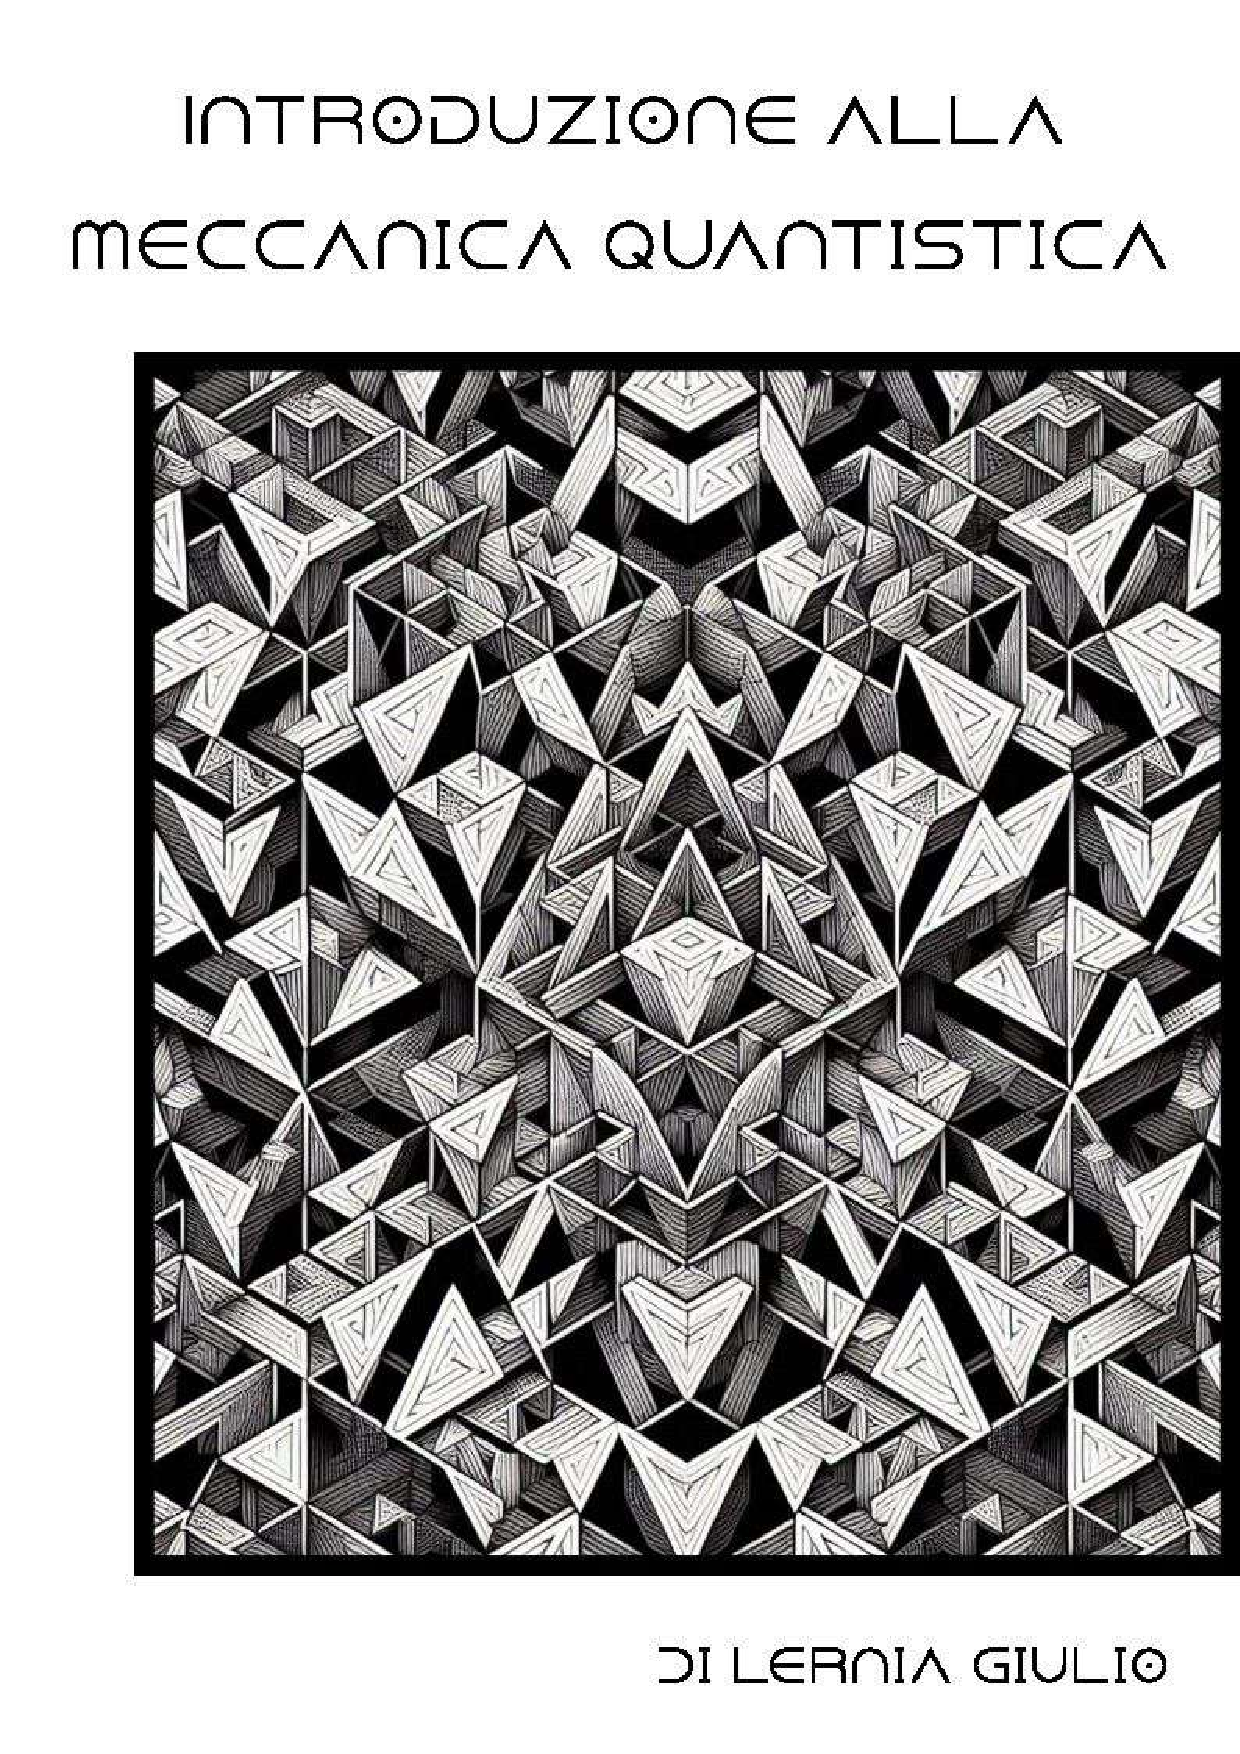
\includepdf{copertina2.pdf}
\tableofcontents
\setcounter{chapter}{0}
\chapter{Meccanica Ondulatoria}
\section{La duale natura della materia}

\subsection{Esperimento della doppia fenditura}
Immaginiamo di condurre un esperimento in cui abbiamo uno spara palline posto difronte ad una parete e tra la parere e il macchinario \'e posto un separatore con due fenditure. Lo spara palline mantiene un certo rateo di fuoco e ruotando su un asse sparge le pallottole su un area angolare molto ampia. Ci aspettiamo che alcune di queste palline passino attraverso le fenditure, dunque posto un rilevatore sulla parete opposta al macchinario ed identificata una regione in cui le palline collidono contro il muro, possiamo domandarci quali sia la probabilit\`a che una pallina colpisca una certa area della superficie complessiva che possiamo indicare come $\Delta x$. Per rispondere a tale domanda costruiamo una distribuzione di probabilit\`a misurando le frequenza relative in un determinato arco di tempo rispetto all'area d'impatto. Ora ipotizziamo che le palline siano indistruttibili e che costituiscano un blocco indivisibile; ovvero se il ritmo con cui spara la macchina diminuisce di molto avremo che in ogni istante di tempo o il muro non viene colpito oppure arriva un solo proiettile. Inoltre la dimensione dei blocchi non dipendono dal rateo di fuoco della spara palline. Dunque possiamo dire che in ogni istante di tempo la dimensione dei blocchi \`e costante e questi sono distinti tra loro. Ripetendo l'esperimento costruiamo una distribuzione di probabilit\`a $P_{12}$ il cui valore \`e dato rispetto alla posizione lungo x. Tale probabilit\`a racchiude sia l'informazione che un proiettile possa passare dal foro 1 che dal foro 2.

 \begin{figure}[!ht]
\vspace{0.1in}
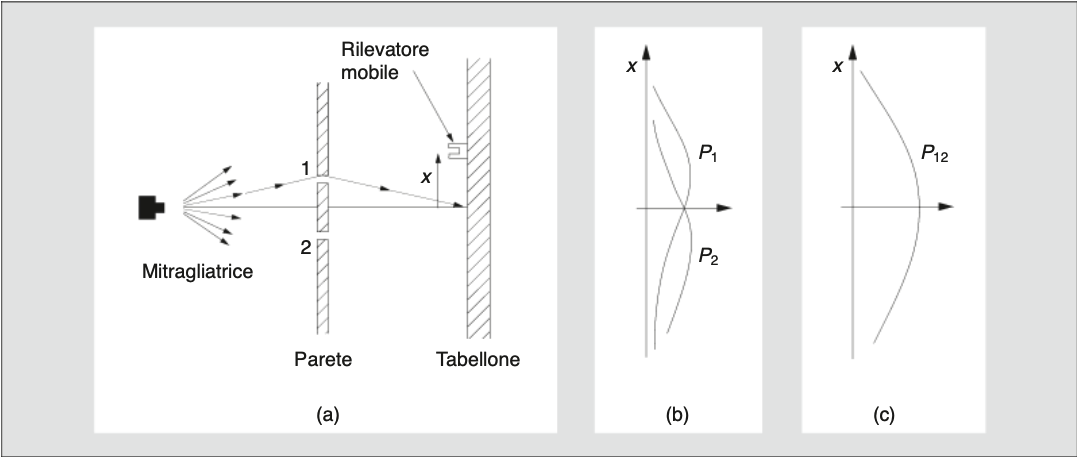
\includegraphics[width =11cm]{palla}	
\centering
\vspace{0.1in}
\caption{}
\end{figure}

\noindent Avremo che la probabilit\`a $P_{12}$ aumenta avvicinandosi a $x = 0$ e diminuisce al suo aumentare. Il fatto che la probabilit\`a sia massima nel centro \`e dovuto al fatto che se chiudiamo per esempio il foro 2 e costruiamo la distribuzione di probabilit\`{a} $P_1$ ripetendo l'esperimento, avremo che questa \`e massima nel punto in cui lo spara pallina mira nel centro della fenditura. Analogamente possiamo definire nello stesso modo chiudendo il foro 1 la probabilit\`{a} $P_2$. Confrontando le figure 1.1.b e 1.1.c si conclude che 
\begin{equation}
	P_{12} = P_1 + P_2
\end{equation}

\noindent Possiamo affermare che la probabilit\`a osservata con entrambe le fenditure \`{e} data dalla somma delle singole probabilit\`a quando una delle due \`e chiusa. Quando osserviamo una condizione di questo tipo diciamo che \textbf{non \`e presente interferenza}.

\subsubsection{Esperimento con Onde}

Ipotizziamo ora di fare lo stesso esperimento, ma anzich\`e utilizzare delle palline usiamo un contenitore d'acqua separato da una parete con due fenditure. A una delle due estremit\`a della scatola in posizione opposta al separatore \`e posto un motore che produce onde circolari. Per semplificare l'esperimento concettuale ipotizziamo che la parete della scatola, opposta la generatore di onde sia un perfetto assorbitore; solidarmente alla parete poniamo un rilevatore che misura l'intensit\`a del moto ondoso. \newline
Il rilevatore registra una grandezza che \`e proporzionale all'energia dell'onda o piuttosto all'energia che giunge al rilevatore.

\ 
\begin{figure}[!ht]
\vspace{0.1in}
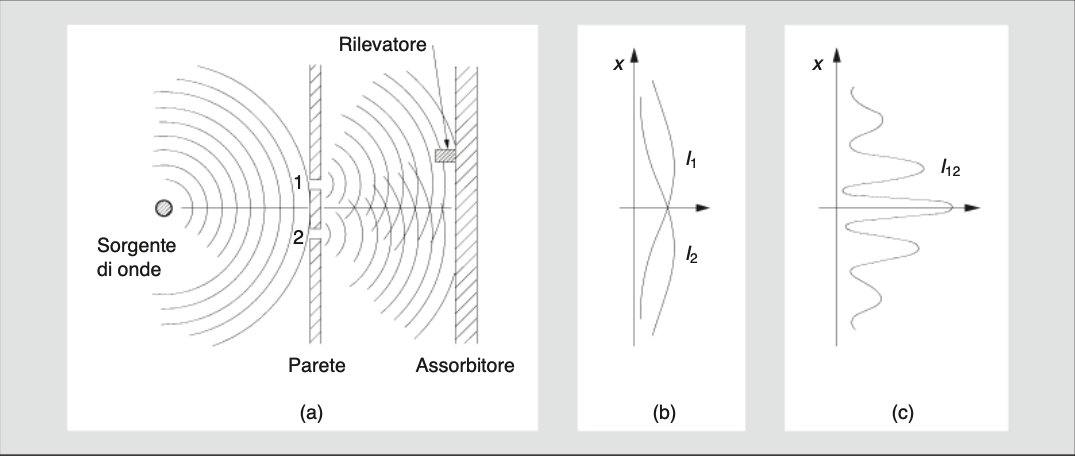
\includegraphics[width = 15cm]{onda}	
\centering
\vspace{0.1in}
\caption{}
\end{figure}

Misurando l'intensit\`a dell'onda per diversi valori di x (mantenedo costante il moto della sorgente delle onde), si ottiene una curva come quella in figura 1.2.c che identifichiamo come $I_{12}$. L'onda originale prodotta dalla sorgente, viene difratta attraverso i fori della parete di mezzo e dunque vengono generante nuove onde circolari con punto di diffusione coincidente con quello dei fori. Chiudendo un foro alla volta come fatto nell'esperimento delle palline si ottengono le singole distribuzioni d'intensit\`{a} rispetto a x date da $I_1$ e $I_2$ e rappresentante in figura 1.2.b. L'intensit\`{a} osservata quando i due fori sono aperti non coincide con la somma delle singole intensit\`a date da uno dei due fori chiusi. In questo caso diciamo che c'\`e \textbf{interferenza} tra le due onde. Dove la curva $I_{12}$ ha i suoi massimi diremo he le due onde sono in fase e i picchi delle onde si sommano, dando luogo a una grande intensit\`a. In tali punti l'interferenza \`e di tipo costruttivo tra le due onde. Un interferenza di questo tipo \`e possibile in tutti i punti dove la differenza delle distanza del rilevatore dai due fori \`e uguale ad un numero intero di lunghezze d'onda.

Nei punti in cui le onde arrivano al rilevatore con una differenza di fase di $\pi$, queste si dicono fuori fase e hanno un interferenza di tipo distruttivo, e l'intensit\`a dell'onda ne risulta diminuita. I valori pi\`u bassi in figura 1.2.c di $I_{12}$ avvengono in quei punti dove c'\`e interferenza distruttiva tra le onde. Si pu\`o dimostrare che i luoghi in cui $I_{12}$ \`e minima \`e nei punti in cui la distanza del rilevatore dal foro 1 differisce dalla distanza dal foro 2 di un numero dispari di lunghezze d'onda.

\noindent L'intensit\`a registrata dal rilevatore peer le onde provenienti da un singolo foro sono propozionali a
\begin{equation}
	I_i \simeq |h_i|^2 
\end{equation}
dove 
\begin{equation}
	h_i = h_ie^{i\omega t} 
\end{equation}
dove il termine $h_i \in \mathbb{C}$. L'intensit\`a rilevata a fenditure entrambe aperte sar\`a proporzionale a 
\begin{equation}
	I_{12} \simeq |h_1 + h_2|^2
\end{equation} 
sviluppando il termine si avr\`a che
\begin{equation}
	I_{12} \simeq |h_1|^2 + |h_2|^2 + 2Re(h_1\overline{h_2})
\end{equation}
L'equazione $I_{12}$ ci dice che $I_{12} \neq I_1 + I_2$ in quanto compare un termine aggiuntivo che descrive il fenomeno d'interferenza.

\subsection{Dualit\`a Onda - particella}

Quanto discusso nei punti precedenti anche se rappresentato da esperimenti concettuali descrive quella che \`e la duale natura della luce. Come sappiamo dalla fisica classica la luce \`e un onda elettromagnetica e come tale viene descritta dall'equazione dell'onda monocromatica
\begin{equation}
	\psi(x,t) = A e^{i(kx - \omega t)}
\end{equation}
e la sua intensit\`a \`e data da 
\begin{equation}
	I \simeq |\psi(x,t)|^2
\end{equation}
ma si comporta anche come una particella priva di massa, ovvero i fotoni. I medesimi risultati valgono anche nel caso di particelle con massa come gli elettroni. 


DESCRIVERE ESPERIMENTO CON ELETTRONI (AGGIUNGERE)

\subsection{La funzione d'onda}
La meccanica quantistica \`e una teoria probabilistica, ovvero si rinuncia all'assunzione della meccanica classica in cui l'evoluzione di un sistema \`e determinata a priori nel momento in cui si conoscono le leggi del moto e le condizioni iniziali di posizione e velocit\`a. Invece si assume che la natura del comportamento di un sistema sia del tutto probabilistica. La meccanica quantistica pu\`o determinare solo probabilisticamente la posizione di una particella nello spazio, ma non pu\`o asserirlo in modo deterministico come nel caso della meccanica classica. Infatti si ha una natura indetermistica dei risultati dovuta alla natura intrinsicamente probabilistica della teoria su cui la meccanica quantistica \`e costruita.

Per un onda di materia la densit\`a di probabilit\`a \`e associata all'intensit\`a con cui si misura l'energia trasportata dall'onda in un punto dello spazio in un tempo fissato $t_0$, ovvero
\begin{equation}
	P(x) = I(x) = |\psi(x,t_0)|^2
\end{equation}
Il termine a destra dell'equazione (1.8) prende il nome di \textbf{ampiezza di probabilit\`a}. Dalla densit\`a di probabilit\`a, \`e possibile calcolare la probabilit\`a effettiva moltiplicandola per il volume: la proobabilit\`a che una particella si trova in un volume infinitesimo dV con centro in un punto $\bold{x}$ \`e data da P($\bold{x},t)dV$.

Nel caso in cui consideriamo il volume esteso la probabilit\`a sar\`a espressa dall'integrale 
\begin{equation}
	P(\bold{x}) = \int_{V}|\psi(\bold{x},t)|^2dV
\end{equation} 
Poich\`e la funzione deve stare in un qualche posto \`e necessario che 
\begin{equation}
	\int_{V}|\psi(\bold{x},t)|^2dV = 1
\end{equation}
dunque la funzione d'onda $\psi(\bold{x},t)$ non pu\`o essere una funzione qualsiasi, ma deve appartenere all'insieme $L^2(\mathbb{R}^3)$ che \`e uno spazio di Hilbert. La condizione posta dall'equazione (1.10) ci dice che la probabilit\`{a} \`e \textbf{normalizzata}. Nel caso in cui si abbia una funzione d'onda per cui 
\begin{equation*}
	\int_{\mathbb{R}^3}dV|\psi(\bold{x},t)|^2 = N < +\infty
\end{equation*}
la funzione d'onda \`e normalizzabile costruendo una funzione d'onda 
\begin{equation*}
	\varphi(\bold{x},t) = \frac{1}{\sqrt{N}}\psi(\bold{x},t)
\end{equation*}
Notare che una funzione d'onda \`e normalizzabile solo se $\psi(\bold{x},t) \to 0 $ abbastanza rapidamente per $\bold{x} \to \infty$.

\noindent Una propriet\`a uitle delle funzioni d'onda \`e data dal risultato che se due funzioni differiscono tra loro per una costante, la fase complessa che li lega fa s\`i che descrivano lo stesso stato
\begin{equation*}
	\psi(\bold{x},t) = e^{i\alpha}\psi(\bold{x},t)
\end{equation*}

per una qualsiasi costante $\alpha \in \mathbb{R}$. In particolare la distribuzione di probabilit\`a rimane invariata. Combinando la condizione di normalizzazione e la non unicit\`a della fase, possiamo pensare agli stati di un sistema come un insieme quoziente formato da funzioni complesse normalizzabili che soddisfano la relazione di equivalenza 
\begin{equation}
	\varphi(\bold{x},t) \sim \psi(\bold{x},t) \iff \psi(\bold{x},t) = \lambda \psi(\bold{x},t) = \varphi(\bold{x},t)
\end{equation}
dove $\lambda \in \mathbb{C}$ e $\lambda \neq 0$. Dove le funzioni $\lambda \psi(\bold{x},t)$ e $\psi(\bold{x},t)$ descrivono lo stesso stato fisico.

\subsection{Principio di Sovrapposizione}
L'insieme delle funzioni d'onda dato da $L^2(\mathbb{R}^3)$ \`e uno spazio di Hilbert e dunque uno spazio vettoriale dotato di prodotto interno. Dunque dati due elementi $\psi_1(\bold{x},t),\psi_2(\bold{x},t) \in L^2(\mathbb{R}^3)$ che rappresenetano due stati del sistema deve esiste anche lo stato
\begin{equation}
	\psi_{3}(\bold{x},t) = \alpha \psi_{1}(\bold{x},t) + \beta \psi_2(\bold{x},t)
\end{equation}
per ogni $\alpha,\beta \in \mathbb{C}$. Tale propriet\`a prende il nome di \textbf{principio di sovrapposizione}. 

\noindent Il principio di sovrapposizione ha importanti conseguenze fisiche. Supponiamo che a un tempo $t_0$ si ha una particella localizzata in prossimit\`a di un punto $\bold{X}$. In accordo con quanto discusso fin'ora la sua posizione sar\`a descritta dalla funzione d'onda Gaussiana
\begin{equation*}
	\psi(\bold{x},t_0) = \frac{1}{\sqrt{N}}e^{-a(\bold{x}-\bold{X})^2}
\end{equation*}
Se applichiamo il principio di sovrapposizione (1.12) avremo che 
\begin{equation*}
	\psi(\bold{x},t_0) = \frac{1}{\sqrt{N'}}\left( e^{-a(\bold{x}-\bold{X}_1)^2}+e^{-a(\bold{x}-\bold{X}_2)^2}\right )
\end{equation*}

per due posizioni arbitrarie $\bold{X_1}$ e $\bold{X}_2$. L'interpertazione di tale equazione ci dice che in qualche modo la particella di si \`e divisa in due e si trova contemporaneamente nei dintorni di $\bold{X}_1$ e $\bold{X}_2$. Dato che una particella \`e indivisibile tale risultato \`e pi\`u interpretabile nel dire che percorre due cammini o pi\`u differenti tra loro simultaneamente.
\section{Particelle e Onde di Materia}

\subsection{Onde di Materia}

Nel 1923 De Broglie formula l'ipotesi che le particelle di materia, come i fotoni, possono avere l'aspetto delle onde. Tale ipotesi viene concepita dallo studio di come gli atomi emettono o assorbono energia (radiazione EM), osservando sperimentale che lo spettro atomico \`e discreto, ovvero \`e costituito da righe spaziate tra loro. Un atomo assorbe o emette fotoni solo a determinate frequenze. Tale risultato \`e facilmente interpretabile nel momento in cui si ipotizza che l'energia degli atomi \`e quantizzata, ovvero l'informazione viene ricevuta in pacchetti di energia che possono assumere solo valori discreti. L'assorbimento o emissione di fotoni fa s\`i che l'energia compia un salto da $E_i$ a $E_j $ tra i livelli di energia permessi. La conservazione dell'energia implica che la frequenza $\nu_{ij}$ di un fotone che genera un salto deve soddisfare la relazione 

\begin{equation}
	h \nu_{ij} = |E_i -E_j|
\end{equation} 
dove il termine "h" prende il nome di \textbf{costante di Planck}.

\noindent Per una particelle di materia di energia E e quantit\`a di moto \textbf{p}, un'onda che possiede una frequenza angolare $\nu = 2\pi \omega$ e un vettore d'onda \textbf{k} valgono le seguenti relazioni
\begin{equation}
\left \{ \begin{array}{l}
	E = h\nu = \hbar \omega \\
	\bold{p} = \hbar \bold{k}
\end{array} \right.
\end{equation}
e la lunghezza d'onda \`e data dall'equazione 

\begin{equation}
	\lambda = \frac{2\pi}{|\bold{k}|} = \frac{h}{|\bold{p}|}
\end{equation}

\subsection{L'equazione di Schr\"odinger}

La funzione d'onda $\psi(\bold{x},t)$ ci fornisce l'informazione sullo stato del sistema. Vogliamo ora capire come questo stato evolva nel tempo. Per studiarne il comportamento introduciamo l'equazione di Schr\"odinger 

\begin{equation}
	\boxed{i\hbar \frac{\partial \psi}{\partial t} = \hat{H} \psi}
\end{equation}
dove la constante $\hbar$ prende il nome di \textbf{costante di Planck ridotta}. Il suo valore \`e 
\begin{equation*}
	\hbar = 1.05 \times 10^{-34} Js
\end{equation*}
In meccanica quantistica l'unit\`a di energia che si utilizza \`e l'elettronvolt (eV), che \`e definito dall'energia cinetica che un elettrone assume quando accelerato da una differenza di potenziale di 1 Volt. Abbiamo che 1 eV $\approx 1,6 \times 10^{-19} J$ e dunque 
\begin{equation*}
	\hbar = 6,58 \times 10^{-16} eVs  
\end{equation*}

In meccanica quantistica l'equazione di Schr\"odinger assume il significato che $\bold{F} = m\bold{a}$ ha nella meccanica classica.
\subsubsection{La Hamiltoniana}

Il termine $\hat{H}$ prende il nome di Hamiltoniana e diverse sue scelte descrivono diversi sistemi fisici. Il cappuccio sulla H, sta ad indicare che nel contesto della meccanica quantistica viene inteso come un operatore che agisce sullo spazio delle funzioni $L^2(\mathbb{R}^3)$. Dato un potenziale $V(\bold{x})$ e assumendo che le particelle non si muovano a velocit\`a relativistiche nello spazio la Hamiltoniana assume la forma
\begin{equation}
	\hat{H} = -\frac{\hbar^2}{2m}\nabla^2 + V(\bold{x})
\end{equation}
che \`e un operatore differenziale. Ovvero prende in pasto una funzione $\psi(\bold{x},t)$ e restituisce un'altra funzione dopo averla differenziata utilizzando l'operatore $\nabla^2$.

\noindent Nel nostro caso la Hamiltonina del sistema coincide con l'energia totale del sistema, ovvero
\begin{equation*}
	H = \frac{\bold{p}^2}{2m} + V(\bold{x})
\end{equation*}
 L'equazione ottenuta in (1.17) \`e data dal fatto che possiamo pensare alla quantit\`a di moto come ad un operatore differenziale
 \begin{equation*}
 	 p \to -i\hbar\nabla 
 \end{equation*}

\subsection{Principio della decomposizione spettrale per una funzione d'onda}

Ipotizziamo di misurare di effettuare una misura al tempo $t_0$ allora la funzione d'onda $\psi(\bold{x},t_0)$ \`e soluzione dell'equazione (1.16) e vale 
\begin{equation*}
	\frac{\hbar^2}{2m}\nabla^2 \psi(\bold{x},t_0) = V(\bold{x})\psi(\bold{x},t_0)
\end{equation*}
essendo $\hat{H}$ un operatore differenziale auto-aggiunto definito sullo spazio di Hilbert $L^2(\mathbb{R}^3)$ possiamo applicare il teorema della decomposizione spettrale. Per un operatore di questo tipo si hanno un numero discreto ( e numerabile) di autovalori, il cui insieme corrisponde alla regione classica in cui il moto \`e limitato (nei punti in cui l'energia cinetica \`e minima si ha inversione), insieme ad uno spettro continuo che contiene tutti quegli autovalori in cui la regione del moto classico non \`e limitata. Di conseguenza la misura $\psi(\bold{x},t_0)$ pu\`o essere scritta come 
\begin{equation}
	\psi(\bold{x},t_0) = \sum_{a}c_{a}\psi_{a} + \int_{\sigma(a)}dE a(e)\varphi_a
\end{equation}
dove $\sigma(a)$ \`e l'insieme dello spetto continuo.

\noindent Nel caso in cui si ha solo uno spettro discreto si ha che per ogni $\psi(\bold{x},t)$, la probabilit\`a $P(a)$ di trovare un autovalore "a" per la misura al tempo $t_0$ \'e data dalla decomposizione di $\psi(\bold{x},t)$ in termini della funzione $\psi_{a}(\bold{x})$
\begin{equation}
	\psi(\bold{x},t_0) = \sum_{a}c_{a}\psi_{a}
\end{equation}
Inoltre per una misurazione $\psi(\bold{x},t_0)$ gli unici valori che pu\`o assumere devono appartenere all'insieme degli autovalori dello spettro discreto dell'operatore H.
Notare che la probabilit\`a deve essere normalizzata e dunque 
\begin{equation*}
	P(a) = \frac{|c_{a}|^2}{\sum_{a} |c_{a}|^2}
\end{equation*}

\newpage 

\subsection{Equazione di Schr\"odinger Indipendente dal Tempo}

L'equazione di Schdr\"odinger (1.16) \'e un equazione alle derivate parziali. Per risolverla consideriamo un asantz in cui la soluzione \'e esprimibile come due componenti di spazio e tempo separate tra loro.
\begin{equation}
	\psi(\bold{x},t) = e^{-\omega t}\psi(\bold{x})
\end{equation}
andando a sostituire nell'equazione (1.16), abbiamo che questa assume la forma 
\begin{equation}
	\hat{H}\psi(\bold{x}) = E\psi(\bold{x}) \quad \text{dove} \quad E = \hbar\omega  
\end{equation}
tale equazione prende il nome di \textit{equazione di Schr\"odinger indipendente dal tempo}. Nelle sezioni successive vedremo che tale equazione ammette autovalori o autostati E, solo per determinati valori. Tali grandezze verrano interpretate come i livelli di energia del sistema.

\noindent Soluzioni della forma (1.20) vengono definiti \textit{stati stazionari}. Come visto nel paragrafo precedente (principio di sovrapposizione) tali stati stazionari possono essere scritti come combinazione lineare di diversi stati stazionari e costituiscono una soluzione generale dell'equazione (1.21).

\subsection{Particella Libera}

Consideriamo una particella nello spazio, non soggetta a forze, allora avremo che il potenziale \`e 
\begin{equation*}
	V(\bold{x},t) = 0 
\end{equation*}
dunque l'equazione di Schr\"odinger pu\'o essere espressa come 
\begin{equation}
	-\frac{\hbar}{2m}\nabla^2 \psi(\bold{x},t) = i\hbar \frac{\partial \psi(\bold{x},t)}{\partial t}
\end{equation}
tale equazione differenziale \`e ha come soluzione la funzione 
\begin{equation}
	\psi(\bold{x},t) = Ae^{i(\bold{k}\cdot\bold{x} - \omega t)}
\end{equation}
 dove A \`e una costante, $\bold{k}$ il numero d'onda. Sostituendo nell'equazione (1.22) questa diventa 
 \begin{equation}
 	\frac{\hbar^2}{2m}\nabla^2 \psi(\bold{x}) = E\psi(\bold{x})
 \end{equation}
dove gli autostati sono delle forma 
\begin{equation*}
	E = \frac{\hbar^2 \bold{k}^2}{2m}
\end{equation*}
dove applicando la condizione di De Broglie si deve avere che 
\begin{equation}
	\omega = \frac{\hbar \bold{k}^2}{2m}
\end{equation}
che lega momento angolare e numero d'onda tra loro. La soluzione (1.23) rappresenta un'onda piana. Se calcoliamo la distribuzione di probabilit\`a associata avremo che 

\begin{equation*}
	P(\bold{x}) = |\psi(\bold{x},t)|^2 = |A|^2
\end{equation*}
e dato che A \`e una costante, si ha che dato un volume dV con centro in $\bold{x}$, la probabilit\`a di misurare la posizione della particella in tale volume \`e uguale in tutto lo spazio considerato.
\newline

\noindent Il principio di sovrapposizione ci dice che una soluzione generale dell'equazione (1.24) \`e combinazione lineare di funzioni d'onda piane che soddisfano la condizione (1.25). Tale soluzione \`e data dalla funzione 

\begin{equation}
	\psi(\bold{x},t) = \frac{1}{(2\pi)^{3 \backslash 2}} \int g(\bold{k})e^{i(\bold{k} \cdot \bold{x}-\omega t)}d^3k
\end{equation}
dove $g(\bold{k})$ pu\`o essere una funzione complessa, a patto che sia sufficientemente regolare affinch\`e la funzione integranda sia integrabile.

\noindent L'equazione (1.26) \`e interpretabile come un \textbf{pacchetto d'onda}, dove il contributo di ciascuna onda monocromatica e piana \`e pesato dalla funzione $g(\bold{k})$. Per t = 0 la funzione d'onda assume la forma 
\begin{equation}
	\psi(\bold{x},0) = \frac{1}{(2\pi)^{3 \backslash 2}} \int g(\bold{k})e^{i\bold{k} \cdot \bold{x}}d^3k
\end{equation}
Si dimostra che la funzione $g(\bold{k})$ non \`e altro che la trasformata di Fourier della funzione $\psi(\bold{x},t)$:
\begin{equation}
	g(\bold{k}) = \frac{1}{(2\pi)^{3 \backslash 2}} \int \psi(\bold{x},0)e^{-i \bold{k} \cdot \bold{x}}d^3x 
\end{equation}

\subsubsection{Significato fisico della funzione g(k)}

Utilizzando le equazioni di De Broglie abbiamo che $\bold{p} = \hbar \bold{k} $ dunque \`e possibile riscrivere la funzione (1.26) rispetto alla quantit\`a di moto come 
\begin{equation*}
	\psi(\bold{x},t) = \frac{1}{(2\pi)^{3 \backslash 2}} \int g(\bold{k})e^{\frac{i}{\hbar}(\bold{p} \cdot \bold{x} - Et)}d^3p
\end{equation*}
dove 
\begin{equation*}
	E = \frac{\bold{p}^2}{2m}
\end{equation*}
di conseguenza la funzione $g(\bold{k})$ diventa in funzione di $\bold{p}$ e si scrive come 
\begin{equation*}
	g(\bold{p}) = \frac{1}{(2\pi)^{3 \backslash 2}} \int \psi(\bold{x},0)e^{-\frac{i}{\hbar}\bold{p} \cdot \bold{x}}d^3x
\end{equation*}
il cui modulo quadrato  esprime la densit\`a di probabilit\`a di misurare un certo momento $\bold{p}$. 
\newline

\noindent Se la distribuzione di probabilit\`a \`e correttamente normalizzata avremo che 
\begin{equation*}
	\int |g(\bold{p})|^2d^3p = \int_{\mathbb{R}^3} | \psi(\bold{x},0)|^2d^3x = 1
\end{equation*}
per le propriet\`a della trasformata di Fourier.
\newpage 

\section{Pacchetti d'onda}
\subsection{Forma di un Pacchetto d'Onda ad un tempo fissato}

Consideriamo una particella libera che si muove in una sola dimensione, ovvero la sua posizione \`e data $x \in \mathbb{R}$. La forma del pacchetto d'onda \`e determinata dalla funzione $\psi(\bold{x},0)$, ovvero dalla misura che effettuiamo in un certo tempo $t=0$ fissato. Consideriamo che la funzione $|g(k)|$ abbia la forma di una distribuzione Gaussiana.

 
\begin{figure}[ht]
\vspace{0.1in}
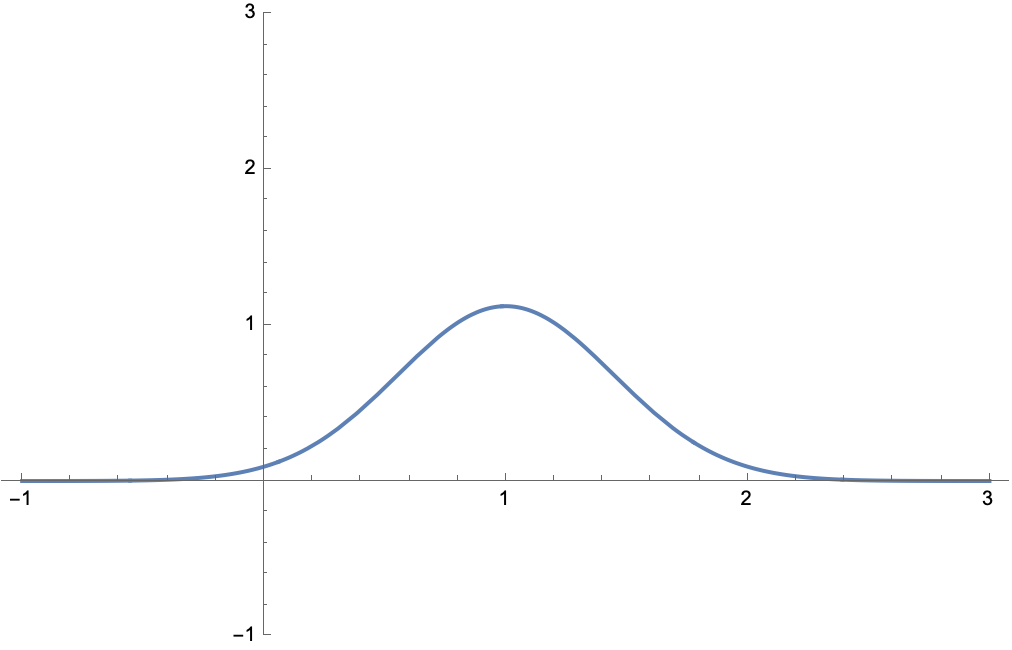
\includegraphics[width = 10cm]{gauss}	
\centering
\vspace{0.1in}
\caption{Grafico della funzione $g(k)$}
\end{figure}

\noindent dove g(k) ha un punto di massimo per $k = k_0$ che in figura 1.3 coincide con $k_0 = 1$ e inoltre la funzione ha ampiezza $\Delta k$ (che per esempio coincide con met\`a della sua ampiezza massima).
Per studiare il comportamento del pacchetto d'onda, consideriamo una caso particolare in cui
\begin{equation}
	\begin{aligned}
\psi(x) & =\frac{g\left(k_0\right)}{\sqrt{2 \pi}}\left[\mathrm{e}^{i k_0 x}+\frac{1}{2} \mathrm{e}^{i\left(k_0-\frac{\Delta k}{2}\right) x}+\frac{1}{2} \mathrm{e}^{i\left(k_0+\frac{\Delta k}{2}\right) x}\right] \\[0.5cm]
& =\frac{g\left(k_0\right)}{\sqrt{2 \pi}} \mathrm{e}^{i k_0 x}\left[1+\cos \left(\frac{\Delta k}{2} x\right)\right]
\end{aligned}
\end{equation}

ovvero la funzione d'onda $\psi(x,0)$ \`e sovrapposizione di un numero finto di funzioni d'onda con ampiezze $1, 1/2$ e $1/2$, dove la funzione d'onda \`e stata perturbata in un intorno di $k_0$. Osserviamo che la funzione (1.29) \`e massima per nel punto x=0, tale risultato \`e dato dal fatto che le onde in tale posizione formano un interferenza costruttiva. Spostandosi dal punto di massimo la funzione decresce fino a quando non raggiunge un punto di minimo dove l'interferenza distruttiva \'e massima; tale punto lo si raggiunge quando le onde hanno una differenza di fase di $\pm \pi$. Siccome la funzione (1.29) \`e una funzione continua, nel passaggio da massimo a minimo esiste sicuramente un punto sull'asse delle ascisse per cui la funzione si annulla, tale punto \'e dato da $x = \pm \frac{\Delta x}{2}$, dove 
\begin{equation}
	\Delta x \Delta k = 4 \pi
\end{equation}
L'equazione (1.30) ci dimostra che pi\`u piccola \`e l'ampiezza della funzione g(k) e maggiore \`e $\Delta x$ della funzione $\psi(x)$.
\newline

\noindent Consideriamo la funzione g(k) della forma \begin{equation*}
	g(k) = |g(k)|e^{i\alpha(k)}
\end{equation*}
assumiamo che $\alpha(k)$ ammetta derivata prima nell'intervallo $\left [k_0-\frac{\Delta k}{2}, k_0 + \frac{\Delta k}{2} \right ]$ allora possiamo sviluppare con Taylor in un intorno di di $k_0$ la funzione $\alpha(k)$

\begin{equation*}
	\alpha(k) \simeq \alpha(k_0) + \frac{d \alpha}{dk} \Big \vert_{k = k_0}(k-k_0)
\end{equation*}
sostituendo nell'equazione (1.27) in una sola dimensione si ha 

\begin{equation}
\psi(x, 0) \simeq \frac{\mathrm{e}^{i\left[k_0 x+\alpha\left(k_0\right)\right]}}{\sqrt{2 \pi}} \int_{-\infty}^{+\infty}|g(k)| \mathrm{e}^{i\left(k-k_0\right)\left(x-x_0\right)} \mathrm{d} k	
\end{equation}

dove il termine $x_0 = -\frac{d \alpha}{dk} \Big \vert_{k = k_0}$.
\newline

\noindent Quando $|x-x_0|$ \`e grande per x fissato, le fasi delle varie funzioni d'onda che formano $\psi(x,0)$ variano rapidamente nel dominio $\Delta k$, e tali onde ti distruggono a vicenda per il fenomeno d'interferenza. Se $x \simeq x_0$, la funzione integrata rispetto a k quasi non ha oscillazione e  $|\psi(x,0)|$ \`e massima.
La posizione $x_M(0) = x_0 $ coincide con il centro del pacchetto d'onda. L'integrale (1.27) assume valore massimo (in termini assoluti) quando le onde hanno l'ampiezza massima ($k \simeq k_0$) e hanno interferenza costruttiva. 
\newline
 
\begin{figure}[ht]
\vspace{0.1in}
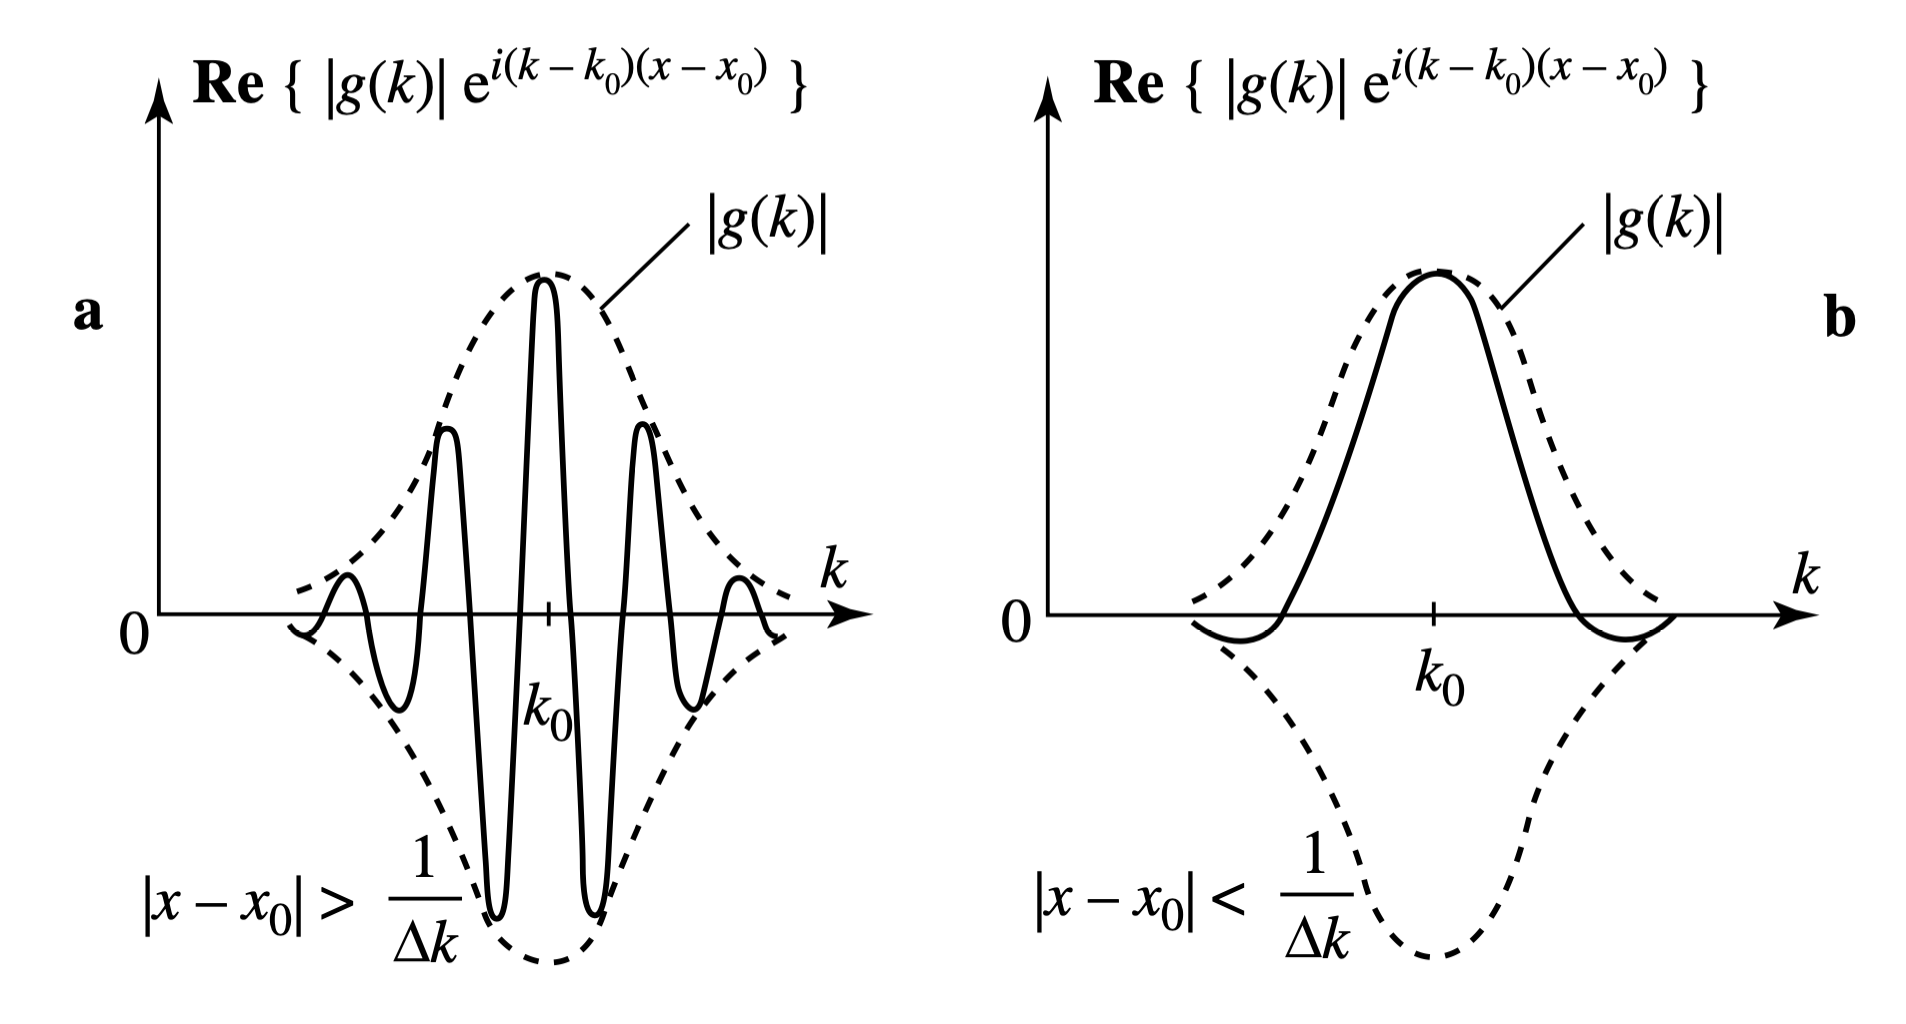
\includegraphics[width = 12cm]{packet}	
\centering
\vspace{0.1in}
\caption{}
\end{figure}

\noindent Quando x si allontana da $x_0$, la funzione $\psi(x,0)$ decresce. La diminuzione diventa significativa nel momento in cui $e^{i(k-k_0)(x-x_0)}$ compie almeno un oscillazione per k nel dominio $\Delta k$, questo accade quando

\begin{equation}
	\Delta k \Delta x \gtrsim 1
\end{equation} 

Tale risultato ci dice che il prodotto $\Delta k \Delta x$ ha un estremo inferiore; il cui valore preciso dipende dalla definizione di $\Delta x$ e $\Delta k$. Una pacchetto d'onda come quello dato dalla funzione (1.27) rappresenta una probabilit\`a, al tempo t=0, pressoch\`e nulla per  una posizione x, al di fuori dell'intervallo $\Delta x $ centrato su $x_0$.


\subsection{Principio d'Indeterminazione di Heisenberg}

Si \`e visto che per un'onda piana $e^{i(k_0x-\omega_0 t)}$ si ha che la densit\`a di probabilit\`a \`e costante in ogni punto dello spazio e in ogni tempo. Tale risultato pu\`o essere interpretato con il fatto che $\Delta x $ assume valore infinito e $\Delta k$ assume valore nullo. Per $k_0$ e $\omega_0$ fissati si ha che energia $E_0 = \hbar \omega_0$ e momento $p_0 = \hbar k_{0}$ sono ben definite. Per un onda piana di questo tipo, la definizione espressa in (1.27) pu\`o essere riscritta interpretando g(k) come una funzione delta
\begin{equation*}
g(k) = \delta(k-k_0) = 
\left \{\begin{array}{l}
	0 \quad k \neq k_0 \\
	+ \infty \quad k = k_0
\end{array} \right.
\end{equation*}
dunque possiamo esprimere la funzione (1.27) come 
\begin{equation*}
	\psi(x) = \frac{1}{\sqrt{2\pi\hbar }}\int \delta(k-k_0)e^{i\frac{p}{\hbar}x}dp = \frac{1}{\sqrt{2\pi \hbar}}
\end{equation*}
e dunque $|\psi(x)|^2 = \frac{1}{2 \pi \hbar}$ costante; di conseguenza la posizione \`e completamente indeterminata e la quantit\`a di moto \`e conosciuta con certezza assoluta.  
\newline

\noindent In termini probabilistici sappiamo che la probabilit\`a di misurare una certa quantit\`a di moto e una certa posizione sono definite dalle grandezze 
\begin{equation*}
	P(x) = \int_{- \infty}^{+\infty} |\psi(x,0)|^2dx \quad \text{e} \quad P(p) = \int_{-\infty}^{+\infty} |g(p)|^2dp
\end{equation*} 

dove le grandezze $\psi(x,0)$ e $g(p)$ sono legate tra loro dalla trasformazione di Fourier. Per tale legame vale il teorema di Plancherel
\begin{equation*}
	P(x) = \int_{- \infty}^{+\infty} |\psi(x,0)|^2dx  = \int_{-\infty}^{+\infty} |g(p)|^2dp
 =P(p)
\end{equation*}
di conseguenza ipotizzando che il valore degli integrali sia C, avremo che al tempo t = 0, misuriamo una probabilit\`a $dP(x) = \frac{1}{C}|\psi(x,0)|^2dx$ che la posizione della particella sia nell'intervallo $[x, x+ \Delta x]$ e nello stesso modo per la quantit\`a di moto che p sia nell'intervallo $[p,p + \Delta p]$.

\noindent Utilizzando le relazioni di De Broglie sappiamo che $\Delta p = \hbar \Delta k$, dunque possiamo riscrivere (1.32) come
\begin{equation}
	\Delta x \Delta p \gtrsim \hbar 
\end{equation}
\newpage 
\noindent Per una particella il cui stato \`e definito dal pacchetto d'onda (1.27), sappiamo che la probabilit\`a della sua posizione al tempo t=0 \`e definito solo in una regione $\Delta x$ con centro $x_0$; la sua posizione \`e conosciuta con una precisione $\Delta x$. Se si misura la quanti\`a di moto allo stesso tempo, il valore $p \in \left [p_0 - \frac{\Delta p}{2}, p_0 + \frac{\Delta p}{2} \right ]$, dato che $|g(p)|^2$ \`e nullo al di fuori di questo intervallo, la quantit\`a $\Delta p$ definisce la precisione con cui conosciamo p. 

\noindent La relazione (1.33) ci dice che fissato un istante di tempo \`e impossibile conoscere con precisione arbitraria la misura della posizione e quanti\`a di moto. Quando si raggiunge il limite inferiore dato da (1.33) aumentare la precisione con cui si conosce la posizione ($\Delta x$ diventa pi\`u piccolo) fa s\`i che la precisione con cui si conosce la quanti\`a di moto diminuisca ($\Delta p $ diventa grande); e viceversa. La relazione (1.33) prende il nome di \textbf{Principio d'indeterminazione di Heisenberg}.

\subsection{Evoluzione di un Pacchetto d'Onda}

Data un'onda piana $e^{i(kx-\omega t)}$ che propaga lungo l'asse Ox con velocit\`a di fase:

\begin{equation*}
	v_f(k) = \frac{\omega}{k}
\end{equation*}
Nel caso un onda elettromagnetica che si propaga nel vuoto la sua velocit\`a di fase \`e \`e costante d \`e data da $v_f = c $ dove c \`e la velocit\`a della luce. Per un onda di questo tipo tutte le onde che costituiscono il pacchetto d'onda si muovo alla stessa velocit\`a, e dunque il pacchetto si muove con la stessa velocit\`a, senza cambiare la sua forma. Nel caso in cui l'onda attraversi mezzi dispersivi, tale risultato non \`e pi\`u vero e la sua velocit\`a di fase \`e data da 
\begin{equation*}
	v_f(k) = \frac{\hbar k}{2m}
\end{equation*}
Tale equazione ci dice la velocit\`a con cui si propaga la singola onda del pacchetto, ma non la velocit\`a nel pacchetto nel suo complesso, per determinare tale grandezza consideriamo la funzione (1.26)

\begin{equation*}
	\psi(x,t) = \frac{1}{\sqrt{2\pi}} \int g(k) e^{i(kx-\omega(k)t)}dk
\end{equation*}

e consideriamo dei coefficienti della forma $g(k) = |g(k)|e^{-i \alpha(k)} $ e riscriviamo la funzione del pacchetto d'onda per un generico periodo t come 
\begin{equation*}
	\psi(x,t) = \frac{1}{\sqrt{2\pi}} \int dk|g(k)|e^{i(kx - \omega(k)t - \alpha(k))} 
\end{equation*}
Vogliamo determinare in quali regioni l'integrale ha un valore diverso da zero, ovvero non si ha interferenza distruttiva per $(x,y) \neq (0,0)$, e per farlo imponiamo la condizione per cui 

\begin{equation}
	\frac{d}{dk} \left [ kx - \omega t - \alpha \right] \approx  0
\end{equation}
risolvendo otteniamo che 
\begin{equation}
	x = \frac{d \omega}{dk}t + \frac{d\alpha}{dk}
\end{equation}
dove la grandezza
 
\begin{equation*}
	v_g = \frac{d \omega}{dk} 
\end{equation*}
prende il nome di \textbf{velocit\`a di gruppo} ed esprime la velocit\`a con cui si propaga il pacchetto d'onda.
Per un'onda di materia si ha che 
\begin{equation*}
	\omega  = \frac{E}{\hbar} = \frac{p^2}{2m \hbar } = \frac{\hbar k^2}{2m }
\end{equation*}
dunque la velocit\`a di gruppo del pacchetto \`e data da 
\begin{equation*}
	v_g = \frac{p}{m}
\end{equation*}

\subsubsection{Esempio - Evoluzione di un pacchetto Gaussiano}

Consideriamo la funzione d'onda rispetto ai momenti 

\begin{equation*}
	\psi(p) = g(p) = C e^{-\frac{\alpha(p-p_0)^2}{\hbar^2}} = Ce^{- \alpha k^2} = g(k)
\end{equation*}
La densit\`a di probabilit\`a dell'evoluto temporale della funzione sar\`a data da 
\begin{equation*}
|\psi(x,t)|^2 = \frac{C}{\sqrt{\frac{\alpha^2}{\hbar^2} + \frac{t^2}{4m^2}}} \exp{\left [ \frac{-\alpha}{4 \alpha^2 + \frac{\hbar^2 t^2}{m^2}}\left ( x - \frac{p_0}{m}t\right)^2\right]}
\end{equation*}
dove il centro del pacchetto d'onda si muove di moto rettilineo uniforme con
\begin{equation*}
	v_g = p_0/m
\end{equation*}
 e nel tempo la Gaussiana di allarga di un fattore 
 \begin{equation*}
 	\sigma(t) \sim \sqrt{4 \alpha^2 + \frac{\hbar^2 t^2}{m^2}}
 \end{equation*}
 
 \section{Comportamento Di un Pacchetto d'Onda In Presenza Di Un Potenziale }
 
 \subsection{Conservazione della probabilit\`a}
 
 Consideriamo una particella soggetta ad un potenziale che V(x,t) che dipende dal tempo, l'equazione di Schr\"odinger avr\`a la forma 
 \begin{equation}
 	i \hbar \frac{\partial \psi}{\partial t} = - \frac{\hbar}{2m} \nabla^2\psi +V(x,t)\psi 
 \end{equation}
tale equazione definisce l'evoluzione nel tempo di funzione d'onda. Le funzioni soluzione risultano essere normalizzate in modo tale che abbiano un interpretazione probabilistica. Vogliamo assicurarci che partendo da una funzione d'onda al tempo $t_0$ il suo evoluto ad un tempo $t > t_0$ ottenuto mediante la funzione (1.36) abbia ancora una descrizione probabilistica. Per dimostrare tale tesi, consideriamo l'evoluzione di $P(\bold{x},t) = |\psi(\bold{x},t)|^2  $ e studiamone l'evoluzione nel tempo
\begin{equation}
	\frac{\partial P}{\partial t}=\psi^{\star} \frac{\partial \psi}{\partial t}+\frac{\partial \psi^{\star}}{\partial t} \psi
\end{equation}
dove $\psi^*$ \`e il complesso coniugato della funzione $\psi$. Consideriamo l'equazione di Schr\"odinger e il suo complesso coniugato
\begin{equation*}
	\frac{\partial \psi}{\partial t}=-\frac{i}{\hbar}\left(-\frac{\hbar^2}{2 m} \nabla^2 \psi+V \psi\right) \quad \text { e} \quad \frac{\partial \psi^{\star}}{\partial t}=\frac{i}{\hbar}\left(-\frac{\hbar^2}{2 m} \nabla^2 \psi^{\star}+V \psi^{\star}\right)
\end{equation*}
 sostituendo nell'equazione (1.37)
 tali risultati si ha che l'evoluto temporale della densit\`a di probabilit\`a nel tempo \`e dato da 
 \begin{equation*}
 	\begin{aligned}
\frac{\partial P}{\partial t} & =\frac{i \hbar}{2 m}\left(\psi^{\star} \nabla^2 \psi-\psi \nabla^2 \psi^{\star}\right) \\[0.4cm]
& =\frac{i \hbar}{2 m} \nabla \cdot\left(\psi^{\star} \nabla \psi-\psi \nabla \psi^{\star}\right)
\end{aligned}
 \end{equation*}
 che riscriviamo nella forma 
 \begin{equation}
 	\frac{\partial P}{\partial t}+\nabla \cdot \mathbf{J}=0
 \end{equation}
 dove il termine $\bold{J}$ prende il nome di \textit{corrente di probabilit\`a} ed \`e dato da 
 \begin{equation}
 	\mathbf{J}=-\frac{i \hbar}{2 m}\left(\psi^{\star} \nabla \psi-\psi \nabla \psi^{\star}\right)ß
 \end{equation}
 Le equazioni della forma (1.38) sono conosciute come \textit{equazioni d continuit\`a} e compaiono quando sono presenti delle grandezze conservate.
 
 \noindent Si consideri un regione di spazio $\Omega \subseteq \mathbb{R}^3$ i cui contorno S. Determiniamo la probabilit\`a che una particella sia trovi in un  qualche punto nella regione $\Omega$ dello spazio, risolvendo l'integrale
 \begin{equation*}
 	P_\Omega(t) = \int_{\Omega} d^3x \; P(\bold{x},t)
 \end{equation*}
 L'equazione di continuit\`a ci dice che tale probabilit\`a cambia nel tempo come
 \begin{equation}
 	\frac{\partial P_\Omega}{\partial t}=-\int_\Omega d^3 x \; \nabla \cdot \mathbf{J}=-\int_S d \mathbf{S} \cdot \mathbf{J}
 \end{equation}
 dove nell'ultima equazione si \`e usato il teorema di divergenza. Dall'equazione (1.40) sappiamo che la probabilit\`a che la particella si trovi in un qualche punto della regione di spazio $\Omega$ cambia solo se \`e presente un flusso di probabilit\`a attraverso il suo contorno S. Se Sappiamo che $\bold{J} = 0$ ovunque sulla superficie S, allora la probabilit\`a che la particella sia nella regione $\Omega $ non cambia e dunque la probabilit\`a \`e costante nel tempo, ovvero
 \begin{equation*}
 	\frac{\partial P_{\Omega}}{\partial t} = 0
 \end{equation*} 
 
 \newpage
 
 \subsubsection{Particella in un potenziale indipendente dal tempo}
 
 Per un potenziale indipendente dal tempo si \`e visto nei paragrafi precedenti che l'equazione di Schr\"odinger (1.21) \`e indipendente dal tempo e che per una soluzione della forma (1.20) si hanno degli stati stazionari, ovvero degli stati dove l'energia del sistema \`e ben definita dato che $E = \hbar \omega$ ed $\omega$ \`e una valore fissato nel tempo per un'onda monocromatica. Essendo l'energia coincidente con la Hamiltoniana e dunque indipendente dal tempo si ha che in meccanica classica questa \`e una grandezza conservata, mentre in meccanica quantistica  si hanno stati di energia ben definiti. Data la forma della soluzione (1.20) la densit\`a di probabilit\`a \`e data da 
 \begin{equation*}
 	|\psi(\bold{x},t)|^2 = |\varphi(\bold{x})|^2
 \end{equation*}
 ovvero \`e indipendente dal tempo.
 
 \noindent Di conseguenza se consideriamo la l'equazione di continuit\`a in (1.38), sapendo che la densit\`a di probabilit\`a \`e indipendente dal tempo l'equazione diventa 
 \begin{equation*}
 	\nabla  \cdot \bold{J} = 0
 \end{equation*}
 dove per una dimensione si ha che 
 \begin{equation*}
 	\frac{\partial J_x}{\partial x} = 0
 \end{equation*}
 ovvero la corrente di probabilit\`a \`e costante.
 
 \subsubsection{Esempio}
 
 Nel caso di un'onda piana $\psi (x) = A e^{\frac{i}{\hbar}px}$ si ha che $|\psi(x)|^2 = |A|^2 $, ovvero la distribuzione di probabilit\`a \`e costante per posizione e tempo. La corrente di probabilit\`a \`e data da 
 \begin{equation*}
 	J = \frac{p}{m}|A|^2 = v|A|^2
 \end{equation*}
 tale risultalto \`e interpretabile come il flusso medio di particelle in una certa regione di spazio.
 
 \subsection{Regioni a potenziale costante}
 
 Consideriamo l'equazione di Schr\"odinger per un potenziale V(x) indipendente dal tempo e per semplicit\`a in una sola dimensione. L'equazione assume la forma 
 \begin{equation}
 	\frac{d}{d^2x}\varphi(x) + \frac{2m}{\hbar}(E-V)\varphi(x) = 0
 \end{equation}
Inoltre ipotizziamo che il potenziale sia costante $V(x) = V_0$ in alcune regione di spazio su cui \`e definito. Le soluzioni dell'equazione (1.41) cambiano in funzione di come cambia la grandezza E-V, dunque dobbiamo fare distinzione tra diverse casistiche:
\begin{enumerate}
	\item Per E  $ >V_0$ introduciamo la costante k data dalla relazione
	\begin{equation*}
		E-V_0 = \frac{\hbar^2 k^2}{2m}
	\end{equation*} 
	la soluzione per l'equazione (1.41) \`e della forma 
	\begin{equation*}
		\varphi(x) = Ae^{ikx}+A'e^{-ikx}
	\end{equation*}
	dove $A,A' \in \mathbb{C}$.
	\item Per $E < V_0$, si ha una condizione che corrisponde ad una regione di spazio che per una particella che segue le leggi della meccanica classica non sarebbe accessibile. In tal caso introduciamo la costante positiva $\rho$ definita da 
	\begin{equation*}
		V_0 - E = \frac{\hbar^2 \rho^2}{2m}
	\end{equation*}
	la soluzione per (1.41) \`e data da 
	\begin{equation*}
		\varphi(x) = Be^{\rho x} + B'e^{-\rho x}
	\end{equation*}
	dove $B,B' \in \mathbb{C}$.
	\item Per $E = V_0$ si ha che $\varphi(x)$ \`e una funzione lineare rispetto x.
\end{enumerate}

\subsubsection{Comportamento della funzione $\varphi(x)$  in punti in cui potenziale \`e discontinuo}

In casi in cui il potenziale \`e una funzione limitata, ma che possiede delle discontinuit\`a con salto, \`e necessario studiare il punto di singolarit\`a e determinare delle condizioni su come collegare i coefficienti delle varie regioni su cui si sono risolte le equazioni. In questi casi si impone che $\varphi(x)$ e $\varphi'(x)$ siano continue nel punto di discontinuit\`a e dunque le soluzioni debbano coincidere in tale punto.

\noindent Riscriviamo l'equazione (1.41) come 
\begin{equation}
	\varphi'' = \frac{2m}{\hbar^2}(V-E)\varphi
\end{equation}
Dato $x_0$ punto di discontinuit\`a per V(x), consideriamo un suo intorno $[x_0 - \varepsilon , x_0 + \varepsilon]$, ed integriamo (1.42) su tale intervallo.
\begin{equation*}
	\int_{x_0 - \varepsilon}^{x_0 + \varepsilon}dx \; \varphi'' = \frac{2m}{\hbar^2} \int_{x_0 - \varepsilon}^{x_0 + \varepsilon} dx \; (V-E)\varphi \; \to 0 \quad \text{per} \quad \varepsilon \to 0
\end{equation*}
tale equazione \`e equivalente ad imporre 
\begin{equation*}
	\varphi'(x_0+ \varepsilon) - \varphi'(x_0 - \varepsilon)  = \varphi'(x_0^+) - \varphi'(x_0^-) \to 0 \quad \text{per} \quad \varepsilon \to 0
\end{equation*}
di conseguenza $\varphi'(x_0)$ \`e continua e quindi anche $\varphi(x_0)$ \`e continua.
 
 \newpage
 
 \subsection{Potenziale a Gradino}
 
 Definiamo un potenziale  come una funzione a gradini
 \begin{equation*}
 	V(x) = \begin{cases}
 		0 \quad x < 0 \\
 		V_0 \quad x> 0 \\
 	\end{cases}	
 	\quad\quad\quad 
 	\vcenter{\hbox{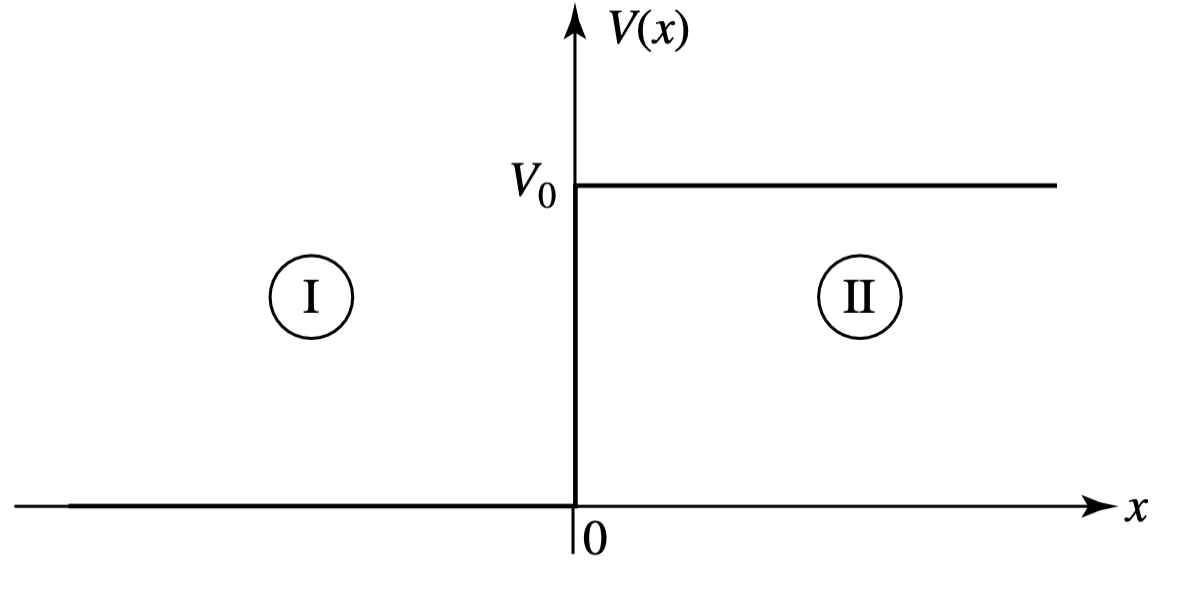
\includegraphics[width=8cm]{gradino}}}
 \end{equation*}
 Immaginiamo di sparare un fascio di particelle da sinistra e osservare che cosa succede. Quello che ci aspettiamo \`e che il fascio rimbalzi indietro se l'energia del fascio \`e minore del potenziale $V_0$, mentre se $E >> V_0$ non ci dovrebbero essere problemi nell'attraversare il gradino e la velocit\`a diminuisce. Per energie leggermente pi\`u grandi $V_0$, si hanno risultati interessanti.
\newline

\noindent  Per la regione (I) dove $x< 0$ consideriamo una soluzione di (1.41) della forma 
\begin{equation*}
	\psi_{1}(x) = Ae^{ik_1x}+A'e^{-ik_1x}
\end{equation*}
doe $k >0$ ed \`e dato da 
\begin{equation*}
	E = \frac{\hbar^2k_1^2}{2m}
\end{equation*}
tale soluzione include una parte della funzione d'onda che rimbalza contro il gradino e continua verso $x \to - \infty$, ma con momento opposto rispetto all'onda iniziale. L'onda entrante $e^{ikx}$ e quella di rimbalzo $e^{-ikx}$ hanno la stessa energia dato che risolvono l'equazione di Schr\"odinger per lo stesso stato, solo che la densit\`a di particelle del differisce, in generale ci aspettiamo che $A' < A$ e dunque parte dell'onda \`e stata assorbita e dunque non tutte le particelle del fascio tornano indietro.
\newline

\noindent Nella regione (II) dove $x > 0 $ e il potenziale vale $V(x) = V_0$, dato che il potenziale \`e costante la soluzione dell'equazione di Schr\"odinger associata \`e data da 
\begin{equation}
	\psi_2(x) = Be^{ik_2x}+B'e^{-ik_2x}
\end{equation}
dove il numero d'onda \`e dato da 
\begin{equation*}
	E-V_0 = \frac{\hbar^2k_2^2}{2m} \quad \Rightarrow \quad  k_2 = \sqrt{\frac{2m(E-V_0)}{\hbar^2}}
\end{equation*}
Si osserva che se l'energia del fascio di particelle \`e maggiore del salto del potenziale, $E > V_0$, il termine $k_2$ \`e reale. Se invece si ha che $E < V_0$, allora $k_2$ \`e un numero immaginario. 

\noindent Da un punto di vista fisico , per $E > V_0$ e dunque $k_2 \in \mathbb{R}$, interpretiamo la componente $Be^{ik_2x}$ della soluzione (1.43) come un onda che si propaga verso destra, mentre il secondo termine $B'e^{-ik_2x}$ \`e un onda che si propaga verso sinistra e che arriva $x \to + \infty$. Il problema \`e che il fascio i particelle arrivare da $x \to - \infty$ e dunque dobbiamo considerare solo soluzioni per cui $B' = 0$.

\noindent Si sarebbe giunti ad una conclusione uguale anche considerando un fascio di energia per cui $E < V_0$, in tal caso $k_2 = i\eta$ dove $\eta > 0$. In questo caso il secondo termine di (1.43) diventa $B'e^{-ik_2x} = B'e^{\eta x}$  che non \`e una funzione normalizzabile per $x \to + \infty$ e dunque soluzioni di questo tipo vengono scartate.
\newline

\noindent Dai risultati ottenuti nei punti precedenti possiamo concludere che la soluzione dell'equazione di Schr\"odinger \`e della forma
\begin{equation}
\psi(x) = \begin{cases}
	Ae^{ik_1x} +A'e^{-ik_1x} \quad x < 0 \\
	Be^{ik_2x} \quad x>0
\end{cases}	
\end{equation}
Per $x = 0 $ la funzione del potenziale V(x) ha un punto di discontinuit\`a con salto, nel paragrafo precedente abbiamo visto che le soluzioni date in (1.44) devono raccordarsi in tale punto e per farlo \`e necessario imporre delle condizioni al contro tali per cui $\psi(x)$ e $\psi'(x)$ siano funzioni continue.
\begin{equation}
	\left \{\begin{array}{l}
		\psi_1(0) = \psi_2(0) \\
		\psi_1'(0) = \psi_2'(0) 
	\end{array} \right.
	\iff
	\left \{ \begin{array}{l}
		A+B = C \\
		ik_1(A-B) = ik_2C
	\end{array}\right.
\end{equation}
Per le analogie della fisica ottica espresse dalle componenti delle soluzioni (1.44), identifichiamo con A la denesit\`a di particelle per il raggio di emissione iniziale, con B quella del raggio riflesso e con C quella del fascio trasmesso. 

\noindent Risolvendo il sistema (1.45) si ottengono i seguenti risultati
\begin{equation}
	B = \frac{k_1 - k_2}{k_1 + k_2}A \quad \text{e} \quad C = \frac{2k_1}{k_1 + k_2}A 
\end{equation}
Tali risultati possiamo interpretarli in termini di corrente di probabilit\`a o da un punto di vista fisico come flusso di particelle. Per il flusso originario si ha che 

\begin{equation*}
	J_{inc} = |A|^2\frac{\hbar k_1}{m}
\end{equation*}
La corrente del raggio riflesso \`e dato da
\begin{equation*}
	J_{rif} = |B|^2\frac{\hbar k_1}{m} = |A|^2\frac{\hbar k_1}{m} \left (\frac{k_1 - k_2}{k_1 + k_2}\right )^2 
\end{equation*}
dove per convenzione il flusso riflesso \`e considerato positivo. Infine il flusso trasmesso \`e 
\begin{equation*}
	J_{trasm} = |C|^2 \frac{\hbar k_2}{m} = |A|^2 \frac{\hbar k_2}{m}\frac{ 4k_1^2}{(k_1 + k_2)^2}
\end{equation*}
Ora ragioniamo su come interpretare questi risultati. Consideriamo il caso in cui $E > V_0$, in modo tale che $k_2 \in \mathbb{R}$. I questo caso le particelle riescono ad attraversare il gradino del potenziale. La domanda \`e come si comportano ? 
\newline

\noindent Per rispondere a tale domanda consideriamo il rapporto tra i flussi. Definiamo

\newpage

\begin{equation*}
	R = \frac{J_{rif}}{J_{inc}} = \left (\frac{k_1 - k_2}{k_1 + k_2} \right )^2
\end{equation*}

e
\begin{equation*}
	T = \frac{J_{trasm}}{J_{inc}} = \frac{4k_1k_2}{(k_1+k_2)^2}
\end{equation*}
tali rapporti prendono rispettivamente il nome di \textit{coefficiente di riflessione } e \textit{coefficiente di trasmissione}. Queste grandezze ci dicono quale frazione del flusso di particelle vengono riflesse e quali vengono trasmesse. In realt\`a dato che stiamo parlando di meccanica quantistica, quello che rappresentano \`e la probabilit\`a che una particella sia trasmessa o riflessa.
\newline

\noindent In particolare per tali coefficienti deve valere l'identit\`a 
\begin{equation*}
	R + T =1
\end{equation*}
che \`e definita per ogni potenziale e ci dice che nessun raggio di particelle viene disperso nell'interazione con il gradino di potenziale.

 
\begin{figure}[ht]
\vspace{0.1in}
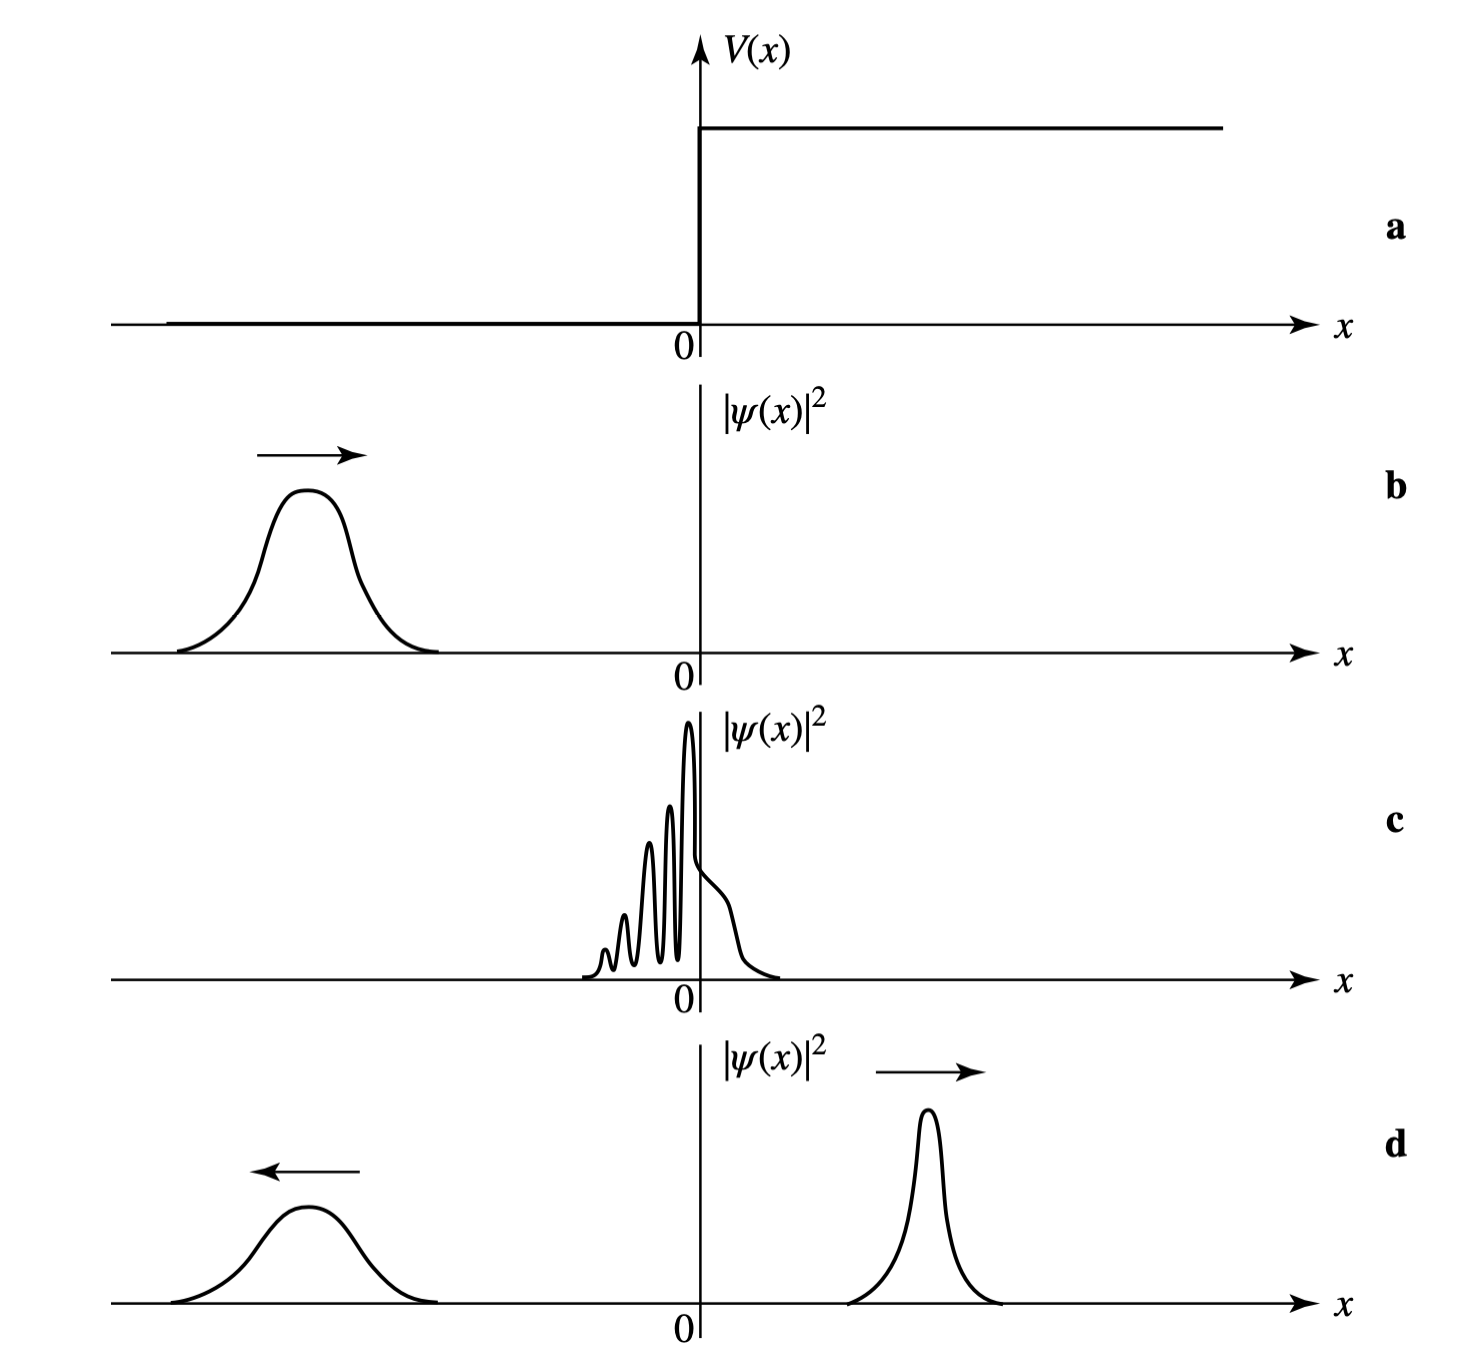
\includegraphics[width = 12cm]{reflect}	
\centering
\vspace{0.1in}
\caption{Si rappresenta il comportamento per un pacchetto d'onda che viene riflesso e trasmesso interagendo un potenziale a gradini per un energia $E > V_0$. Si osserva che il pacchetto riflesso ritorna con meno energia e una forma pi\`u schiacciata, ma con la stessa ampiezza del pacchetto originale. Mentre il pacchetto trasmesso ha una forma pi\`u piccata rispetto a quello di origine e una larghezza minore. Rispettivamente uno si propaga verso sinistra e l'altro verso destra.}
\end{figure}

\newpage

Resta da discutere il comportamento del raggio di particelle nel caso in cui $0< E < V_0$. In questo caso si ha che $k_2 \in \mathbb{C}$ e possiamo esprimerlo come $k_2 = i \eta$. Dunque la soluzione dell'equazione di Schr\"odinger per la regione del piano dove $x > 0$ diventa $\psi(x) = Be^{-\eta x}$, onde di questo tipo prendono il nome di onde evanescenti. Ripetendo quanto fatto per $E > V_0$ si ha che il coefficiente di trasmissione $T = 0$ e si ha $R=1$. Ovvero il fascio viene solo riflesso.
\newline

\noindent In realt\`a esistendo una soluzione reale nella regione del piano per $x > 0$ esiste una piccola probabilit\`a che il pacchetto d'onda possa attraversare un minimo la barriera per poi venire riflesso.

\subsection{Barriera di Potenziale (Effetto Tunnel)}
Dato il seguente potenziale limitato

 \begin{equation*}
 	V(x) = \begin{cases}
 		V_0 \quad 0< x < l \\
 		0 \quad \text{altrimenti} \\
 	\end{cases}	
 	\quad\quad\quad 
 	\vcenter{\hbox{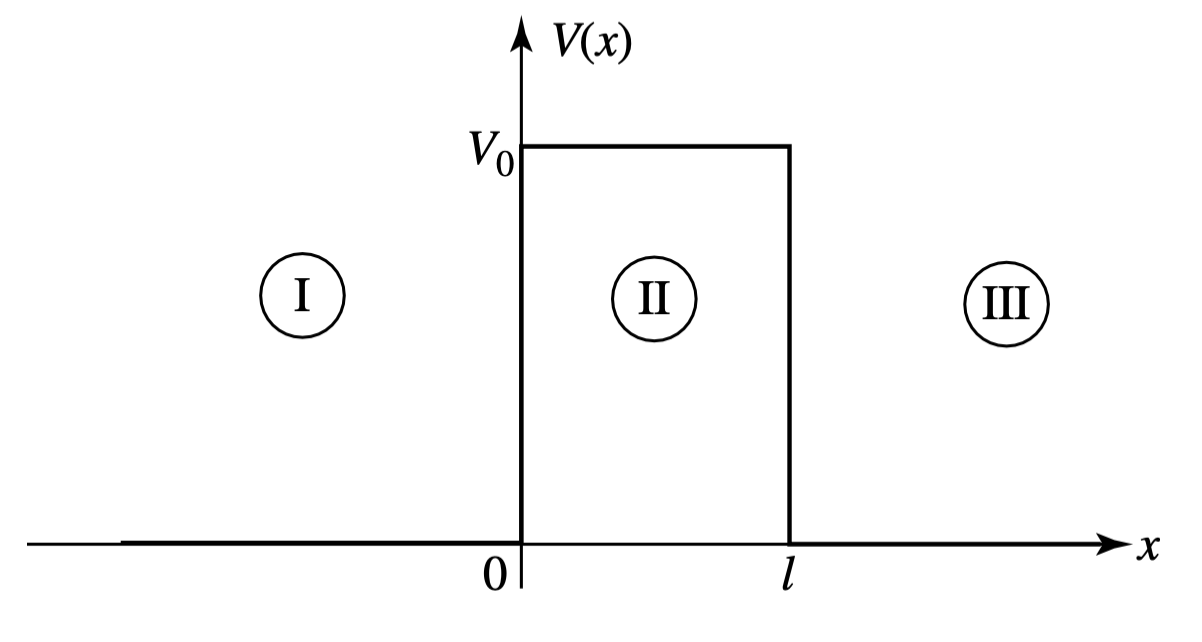
\includegraphics[width=8cm]{tunnel}}}
 \end{equation*}
 dove $V_0 > 0$. Il procedimento per risolvere l'equazione di Schr\"odinger \`e analogo a quello usato per il gradino del potenziale. L'unica differenza \`e che si ragione su 3 partizioni del piano e si determinato le soluzioni su di esse, per poi raccordarle nei punti di discontinuit\`a $x_1 = 0$ e $x_2 = l$ imponendo la condizione di continuit\`a per $\psi(x)$ e $\psi'(x)$. 
 
 \noindent Consideriamo l'energia per $E > V_0$, le soluzioni sono della forma 
 
 \begin{equation}
 	\psi(x) = \begin{cases}
 		A_1e^{ik_1x} + A_1'e^{-ik_1x} \quad x < 0\\
 		A_2e^{ik_2x} + A_2'e^{-ik_2x} \quad  0<x<l \\
 		A_3e^{ik_1x}
 	\end{cases}
 \end{equation}
 osserviamo che nella terza regione $k_1 = k_3$, dato che rispettivamente 
 \begin{equation*}
 	k_1 = k_3 = \sqrt{\frac{2mE}{\hbar^2}} \quad \text{e} \quad k_2 = \sqrt{\frac{2m(E-V_0)}{\hbar^2}}
 \end{equation*} 
 applicando le condizioni al contorno nei punti di discontinut\`a del potenziale, dopo alcuni passaggi algebrici otteniamo i coefficienti di riflessione e trasmissione 
 \begin{equation*}
 	R = \left |\frac{A_1'}{A_1} \right |^2 = \frac{(k_1^2 - k_2^2)sin^2(k_2l)}{4k_1^2k_2^2 + (k1^2-k_2^2)sin^2(k_2l)}
 \end{equation*}
 e
 \begin{equation*}
 	T = \left | \frac{A_3}{A_1} \right |^2 = \frac{4k_1^2k_2^2}{4k_1^2k_2^2 + (k1^2-k_2^2)sin^2(k_2l)}
 \end{equation*}
 \newpage 
 
 \noindent La probabilit\`a di riflessione oscilla al variare di $k_2$(ovvero dell'energia) e per $sin(k_2l) = 0 $ si ha T = 1.
 
 \noindent Nel caso in cui l'energia $0<E<V_0$ si ha che $k_2 = i\eta$ dove $\eta \in \mathbb{R}^+$ e dunque possiamo riscrivere il coefficiente di trasmissione come 
 \begin{equation*}
 	T = \frac{4k_1^2\eta^2}{4k_1^2\eta^2 + (k_1^2 + \eta^2)sinh^2(\eta l)}
 \end{equation*}
 Osserviamo che la probabilit\`a che la particella attraversi la barriera di potenziale non svanisce, tale risultato \`e in contrasto con la visione classica in cui il fascio di particelle dovrebbe essere solo riflesso. Tale fenomeno prende il nome di \textit{effetto tunnel}.
 \newline
 
 \noindent Per valori di $V_0 >> E$ o l molto grande si ha che $T \to 0$. L'effettp tunnel \`e importante per la descrizione dei fenomeni di decadimento radioattivo.
 
 \subsection{Buca di Potenziale dalle Pareti Infinitamente Grandi}
 
 Prendiamo in esame un potenziale della forma 
 \begin{equation*}
 	V(x) = \begin{cases}
 		0 \quad \text{altrimenti}\\
 		+ \infty \quad x \notin [0,a]
 	\end{cases} 
 	\quad \quad 
 	\vcenter{\hbox{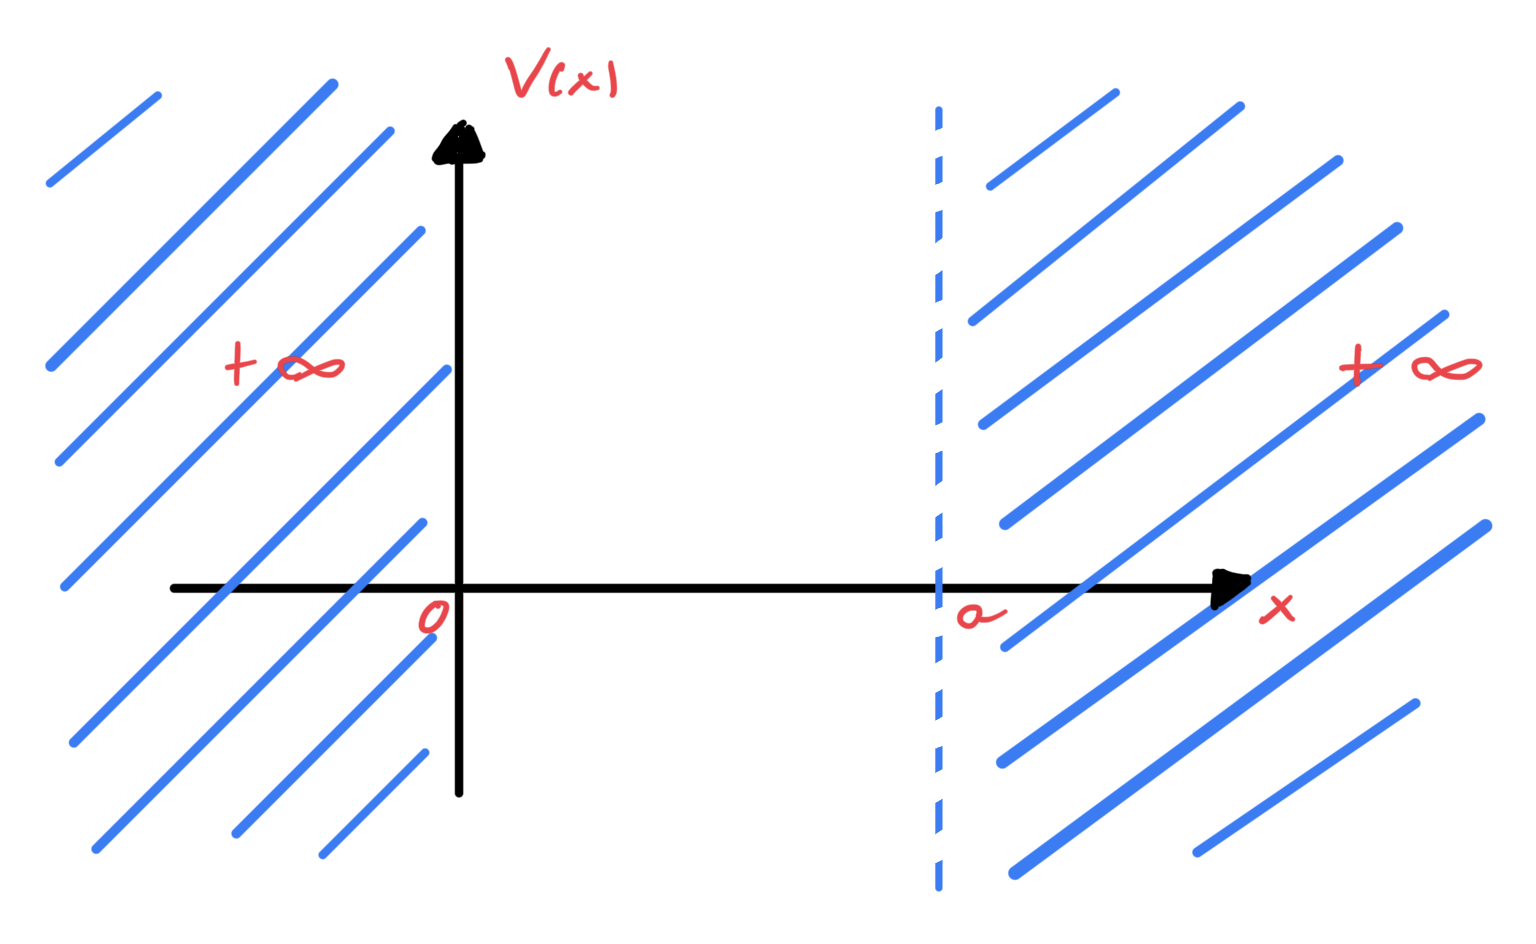
\includegraphics[width=9cm]{infinitewell}}}
 \end{equation*}
 e prendiamo in esame una particella trappola all'interno della buca di potenziale di larghezza "a" e pareti infinite. L'equazione di Schr\"odinger assume la forma 
 \begin{equation*}
 	-\frac{\hbar^2}{2m}\frac{\partial^2 \psi}{\partial x^2} + V(x)\psi = E \psi
 \end{equation*}
 Se vogliamo considerare solo stati di energia finiti, necessariamente avremo che per le regioni del piano in cui $V(x) = + \infty$ la funzione d'onda deve essere della forma $\psi(x) = 0$. Nella regione di spazio in cui il potenziale \`e nullo ritroviamo l'equazione che descrive l'evoluzione di una particella libera.
 \begin{equation}
 	-\frac{\hbar^2}{2m}\frac{\partial^2 \psi}{\partial x^2}  = E \psi
 \end{equation}
 Come fatto per la discussione dei potenziali precedenti dovremmo imporre la condizione che per $x = 0$ e $x = a$ la funzione d'onda $\psi(x) = 0$. Di conseguenza le funzioni d'onda saranno una restrizione della classe delle generiche funzione d'onda $e^{ikx}$. Consideriamo come ansatz di (1.48) la funzione 
 \newpage
 
 \begin{equation*}
 	\psi(x) = Ae^{ikx} + Be^{-ikx}
 \end{equation*}
con $k >0$. Imponendo la condizione $\psi(0) = 0$ sul bordo della buca del potenziale otteniamo le condizioni $B = -A$, dunque l'equazione precedente assume la forma 
\begin{equation*}
	\psi(x) = A(e^{ikx}-e^{-ikx}) = 2iA\sin(kx)
\end{equation*}
Il termine $2iA$ \`e una costante di normalizzazione e non influisce sulla descrizione della fisica del sistema. Imponendo la seconda condizione in cui $\psi(a) = 0$,abbiamo che 
\begin{equation*}
	\sin(ka) = 0 \Rightarrow k = \frac{n\pi}{a} \quad \text{per} \quad n \in \mathbb{Z}^+
\end{equation*}
 Per normalizzare la funzione calcoliamo
 \begin{equation*}
 	\int_0^a |\psi(x)|^2 = 1 \Rightarrow \int_0^a dx \; \sin^2 \left (\frac{n \pi x}{a} \right) = \frac{a}{2} \Rightarrow A = \frac{-i}{2}\sqrt{\frac{2}{a}}
 \end{equation*}
 e dunque la soluzione normalizzata diventa 
 \begin{equation}
 	\psi_n(x) = \sqrt{\frac{2}{a}}\sin\left (\frac{n \pi x}{a} \right )
 \end{equation}
 sostituendo all'interno dell'equazione (1.48) si ha che l'energia \`e quantizzata, ovvero pu\`o assumere valori solo su uno spettro di stati discreto.
 \begin{equation}
 	E_n = \frac{\hbar^2k_n^2}{2m} = \frac{\hbar^2 (n \pi)^2}{2ma^2}
 \end{equation}
 Quando una particella \`e vincolata a muoversi in regioni di spazio limitate, i livelli di energia si quantizzano perch\`e si formano delle onde stazionarie.
 
\begin{figure}[ht]
\vspace{0.1in}
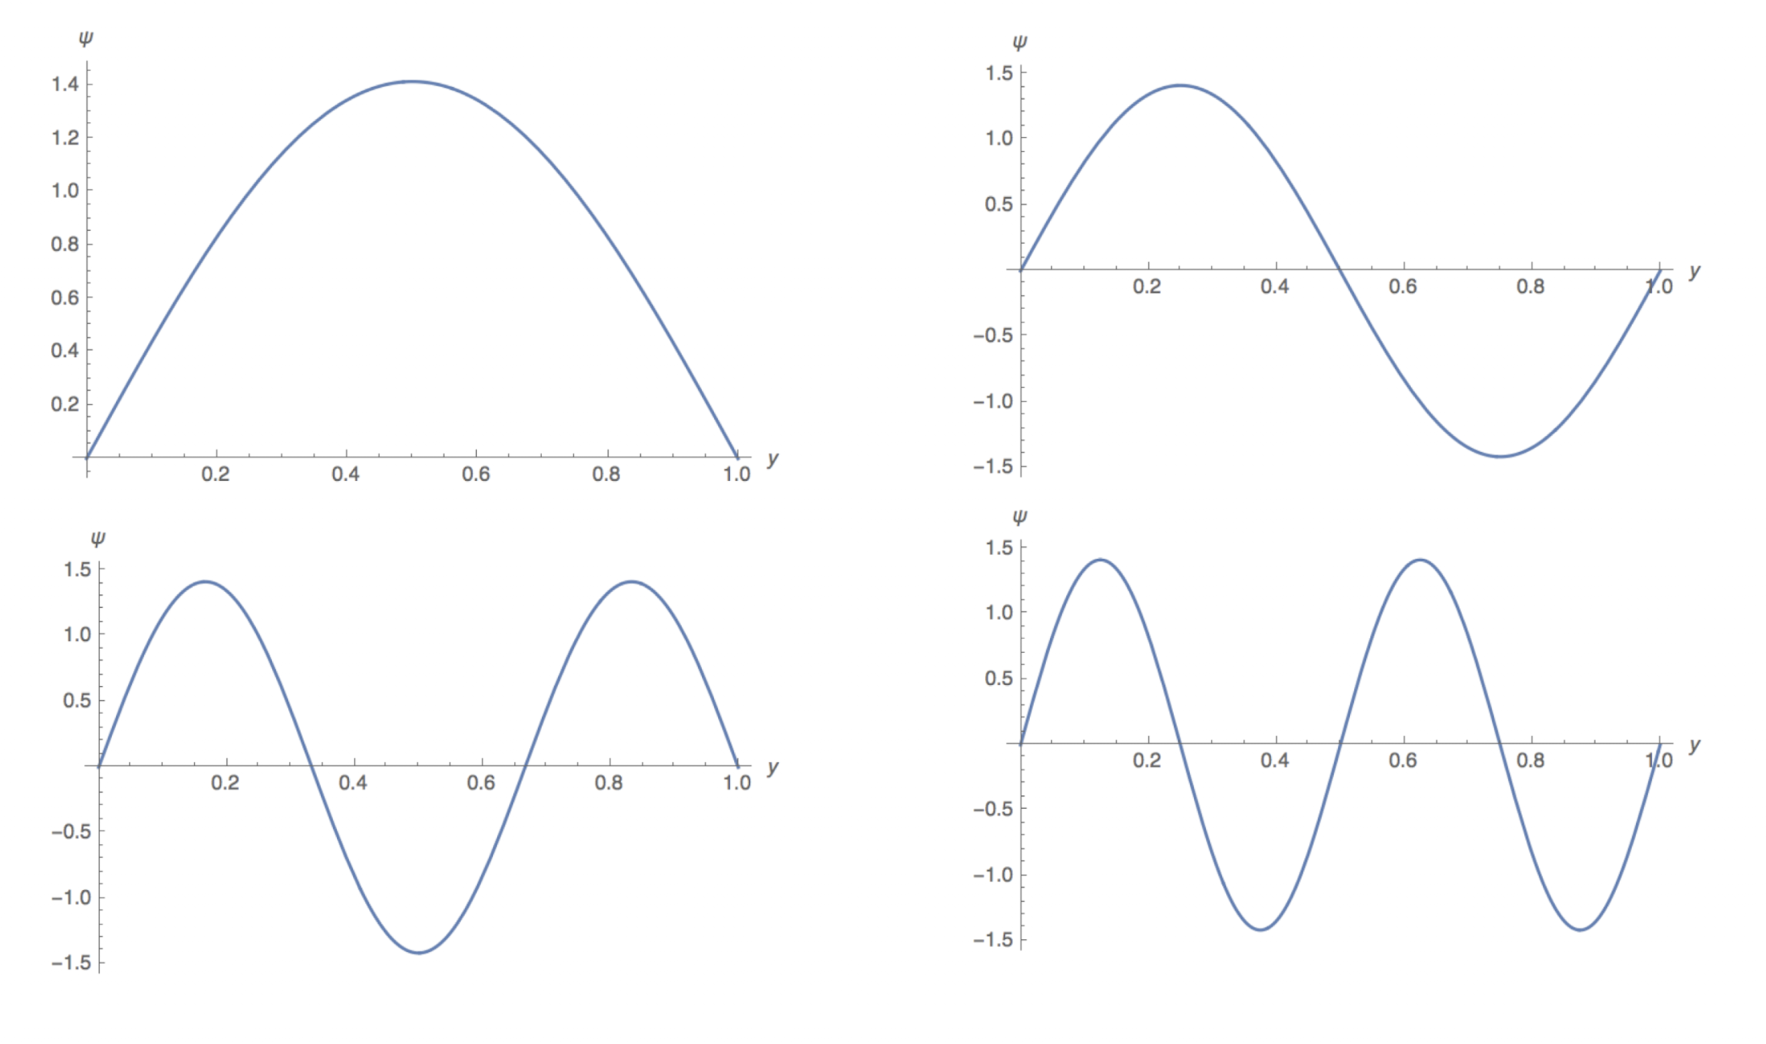
\includegraphics[width = 12.6cm]{groundstate}	
\centering
\vspace{0.1in}
\caption{funzioni d'onda stazionarie per n = 1,2,3,4.}
\end{figure}

\subsubsection{Propriet\`a di superposizione per gli stati stazionari}
Abbiamo che gli $E_n$ definiti dalla relazione (1.50) sono numeri reali e costituiscono gli autovalori dell'operatore Hamiltoniano H, di conseguenza le funzione d'onda $\psi_n(x)$ sono i corrispettivi autostati. Dunque $\{\psi_n(x)\}_{n \in \mathbb{N}}$ \`e una base ortonormale dello spazio $L^2([0,a])$, quindi una qualsiasi funzione $\psi(x)$ pu\`o essere scritta come combinazione lineare degli elementi della base 
\begin{equation}
	\psi(x) = \sum_{n=1}^{+ \infty}c_n \psi_n(x)
\end{equation}
dove i $c_n$ sono i coefficienti normalizzati. Essendo H un operatore lineare la funzione $\psi(x)$ espressa come nell'equazione (1.51) \`e soluzione dell'equazione di Schr\"odinger.
\newline

\noindent Come intuibile la particella rimane vincolata all'interno del pozzo, dunque possiamo pensare che le onde stazionarie che la rappresentano si muovano avanti e indietro all'interno delle pareti; di conseguenza la quantit\`a di moto non \`e ben definita in quanto $\psi(x) = e^{ikx} - e^{-ikx}$ e dunque \`e sovrapposizione di due stati che rappresentano rispettivamente due quantit\`a di moto distinte $p = \hbar k$ e l'altra $p = - \hbar k$.

\subsection{Buca di Potenziale Limitata}

Dato il potenziale 
\begin{equation*}
	V(x) = \begin{cases}
		-V_0 \quad x \in \left [-\frac{a}{2}, \frac{a}{2} \right ] \\
		0 \quad \text{altrimenti}
	\end{cases}
	\quad\quad\quad 
 	\vcenter{\hbox{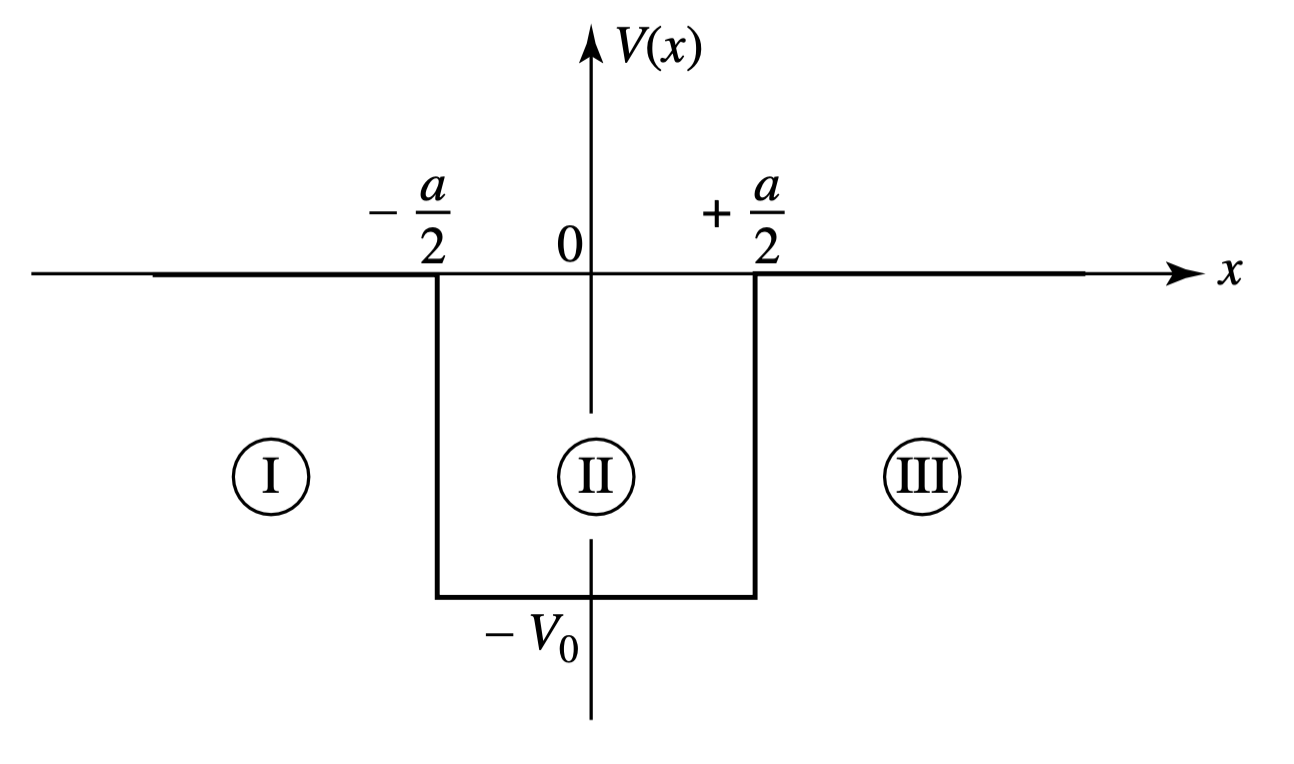
\includegraphics[width=8cm]{square}}}
\end{equation*}
dove $V_0 > 0$. Prima di proseguire con la ricerca della soluzione per l'equazione di Schr\"odinger associata, osserviamo che il potenziale \`e una funzione pari, ovvero V(-x) = V(x), questo vuol dire che tutte le soluzioni o sono funzioni pari o funzioni dispari. Osserviamo che se $\psi(x)$ \`e soluzione dell'equazione, allora anche $\psi(-x)$ deve esserlo, e dato che le soluzioni sono univoche e non possono esserci livelli di energia degeneri (ovvero un medesimo livello di energia associato a due funzioni distinte) dobbiamo avere che 
\begin{equation*}
	\psi(x) = \alpha \psi(-x)
\end{equation*}
per $\alpha \in \mathbb{C}$. Abbiamo che 
\begin{equation*}
	\psi(x) = \psi(-(-x)) = \alpha\psi(-x) = \alpha^2\psi(x)
\end{equation*}
dunque $\alpha = \pm 1$, di conseguenza la funzione pu\`o essere solo pari o dispari.

\subsubsection{Funzioni D'onda Pari}

Cerchiamo soluzioni per gli stati legati, per cui al di fuori del pozzo di potenziale abbiano la forma:
\begin{equation*}
\psi(x) = 
\begin{cases}
	Ae^{-i\eta x} \quad x > \frac{a}{2}\\
	Ae^{i\eta x} \quad x < -\frac{a}{2}
\end{cases}
\end{equation*}
dove $\eta \in \mathbb{R}^+$, scegliamo tali soluzioni in quanto vogliamo che la funzione d'onda sia una funzione $\psi \in L^2 \left (\left (-\infty,-\frac{a}{2} \right ] \cup \left [\frac{a}{2}.+ \infty \right )\right )$. Ci interessa sapere quali valori possa avere $\eta$ dato che questo determina l'energia degli stati legati, $E = -\frac{\hbar^2 \eta^2}{2m}$.
\newline 

\noindent All'interno dell'intervallo in cui il potenziale \`e non nullo, l'equazione di Schr\"odinger assume la forma
\begin{equation*}
	-\frac{\hbar^2}{2 m} \frac{d^2 \psi}{d x^2}=\left(E+V_0\right) \psi \quad -\frac{a}{2}<x< \frac{a}{2}
\end{equation*}
In base al valore dell'energia abbiamo due diversi tipi di soluzione 
\begin{itemize}
	\item Se $E < -V_0$ si hanno funzioni d'onda della forma $e^{\pm \rho x}$
	\item Se $E > -V_0$ si hanno funzioni d'onda della forma $e^{\pm ikx}$
\end{itemize}
Le soluzioni che ci interessano sono quelle per cui abbiamo gli stati legati e dunque ci limitiamo a studiare il comportamento del sistema per $-V_0 <E < 0$.

\noindent Dato che stiamo cercando soluzioni pari la funzione d'onda \`e data dalla combinazione lineare $\psi(x) = e^{ikx} + e^{-ikx}$ e dunque 
\begin{equation*}
	\psi(x) = B\cos(kx) \quad |x| < \frac{a}{2}
\end{equation*}
Non ci resta che applicare le condizioni al contorno per determinare le costanti di normalizzazione A e B. Dato che le funzioni dentro e fuori dalla buca sono pari \`e sufficiente applicare solo che condizioni per $\psi(-\frac{a}{2})$ e $\psi'(-\frac{a}{2})$, ottenendo
\begin{equation*}
\begin{cases}
	Ae^{-\eta \frac{a}{2}} = B \cos \left (\frac{a}{2}k \right ) \\
	kB \sin \left ( \frac{a}{2}k \right) = A\eta e^{-\eta \frac{a}{2}} 
\end{cases}
\end{equation*}
facendo il rapporto tra le funzioni abbiamo che 
\begin{equation*}
	\eta = k \tan \left (k \frac{a}{2} \right ) \iff \tan \left (k \frac{a}{2} \right ) = \frac{\eta}{k}
\end{equation*}
vogliamo determinare l'esistenza delle soluzioni al variare di k. Riscriviamo il termine di destra osservando che $k_0^2 = \frac{2mV_0}{\hbar^2}$ e dunque un generico stato k, possiamo scriverlo come $k^2 = k_0^2 - \eta^2$ e quindi
\begin{equation}
	\tan \left( \frac{a}{2}k \right ) = \sqrt{\frac{k_0^2 - k^2}{k^2}} = \sqrt{\left (\frac{k_0}{k} \right )^2 -1}
\end{equation}
essendo (1.52) un equazione trascendentale questa non ammette soluzioni esplicite, dunque si ricorre al metodo grafico per verificare l'esistenza di almeno una soluzione.

\newpage 
 
\begin{figure}[!ht]
\vspace{0.1in}
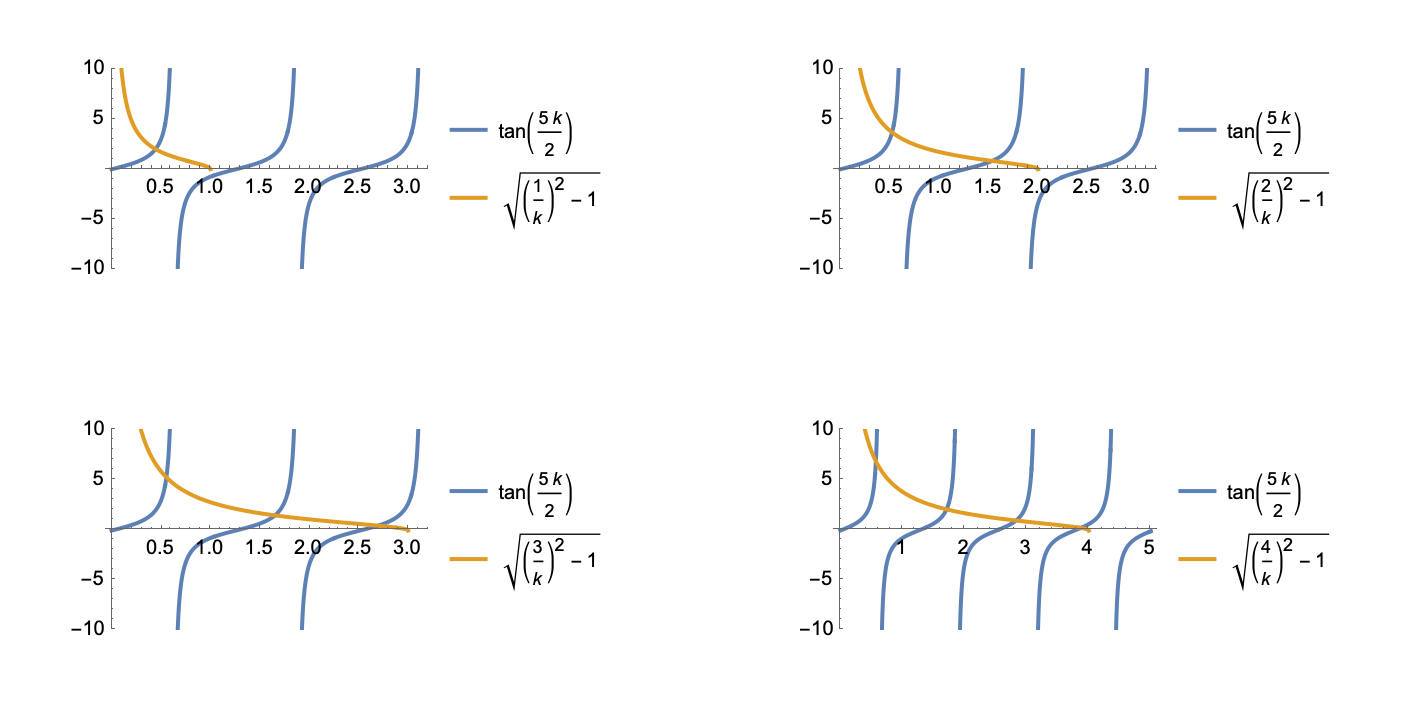
\includegraphics[width = 17cm]{k0}	
\centering
\vspace{0.1in}
\caption{Esistenza delle soluzioni al variare di $k_0 = 1,2,3,4$ e per una buca di ampiezza 5.}
\end{figure}
Come si osserva in figura 1.7 all'aumentare di $k_0$ e dunque del potenziale, il numero di soluzioni cresce. Per $V_0 \to + \infty$ si hanno un infinit\`a di soluzioni. Inoltre il numero di soluzioni dipende anche dalla costante "a" in quanto i punti in cui la tangente diverge ad infinito sono dati da $ k = \frac{n\pi}{a}$ per $n \in \mathbb{N}$. Infatti aumentando il valore di "a" abbiamo che le curve dipendenti da $k_0$ restano fisse, ma intersecano in pi\`u punti la funzione.
\newline

\noindent Il numero di stati legati \`e dato dalla relazione 
\begin{equation*}
	\frac{n\pi}{a} \leq k_0 \leq \frac{(n+1)\pi}{a}
\end{equation*} 
tale condizione \`e esprimibile rispetto al potenziale come
\begin{equation*}
	\frac{(n \pi)^2 \hbar^2 }{2ma^2} \leq V_0 \leq \frac{(n+1)^2 \pi^2 \hbar^2}{2ma^2}
\end{equation*}
Abbiamo visto che per livelli di energia $-V_0<E<0$ si hanno degli stati legati, e questo \`e quello che ci aspettiamo da un punto di vista classico per una particella confinata di una buca di potenziale. La parte interessante \`e che al di fuori della buca sono presenti delle funzioni d'onda decrescenti e questo vuol dire che per regioni che classicamente sarebbero inaccessibili si ha una probabilit\`a finita di trovare la particella al di fuori della buca.
\newpage 

\subsubsection{Funzioni d'onda dispari}
Analogamente a quanto fatto per le funzioni pari, al di fuori della buca di potenziale ricerchiamo delle funzioni della forma 
\begin{equation*}
\psi(x) = 
\begin{cases}
	Ae^{-\eta x} \quad x > \frac{a}{2}\\
	-Ae^{\eta x} \quad x < -\frac{a}{2}
\end{cases}
\end{equation*}
mentre all'interno della buca si ha una funzione della forma 
\begin{equation*}
	\psi(x) = B\sin(kx) \quad |a| < \frac{a}{2}
\end{equation*}
raccordando le soluzioni in $x = \frac{a}{2}$ si ottengono le condizioni al contorno
\begin{equation*}
	\begin{cases}
B \sin \left( k \frac{a}{2} \right ) = A e^{-\eta \frac{a}{2}} \\
k B \cos \left (k \frac{a}{2} \right)   =-\eta A e^{-\eta \frac{a}{2}}
\end{cases}
\end{equation*}
facendone il rapporto otteniamo
\begin{equation*}
	\cot \left (k \frac{a}{2} \right) = - \frac{\eta}{k} = - \sqrt{\left (\frac{k_0}{k}\right)^2 -1}
\end{equation*}
In questo caso non c'\'e garanzia dell'esistenza della soluzione. Essa esiste solo se il potenziale \`e profondo abbastanza o la buca larga a sufficienza.

\subsection{Potenziale a Funzione Delta}

Definiamo potenziale a funzione delta la seguente espressione
\begin{equation*}
	V(x) = -V_0\delta(x)
	\quad\quad\quad\quad\quad 
 	\vcenter{\hbox{\includegraphics[width=8cm]{delta}}}
\end{equation*}
dove $V_0 > 0 $. La funzione delta anche se definita in questo modo non \`e realmente una funzione, ma \`e una distribuzione che soddisfa le condizioni
\begin{equation*}
	\delta(x) = 
	\begin{cases}
		+ \infty \quad x  =  0\\
		0 \quad\quad\;  x \neq 0
	\end{cases}
	\quad \text{e} \quad \int_{-\infty}^{+\infty}dx\;\delta(x) =1
\end{equation*}
La discontinuit\`a data dalla funzione delta \`e molto pi\`u significativa di quella che si \`e vista per i potenziali con salto. Come fatto nei paragrafi precedenti per studiare il comportamento delle soluzioni in un intorno della discontinuit\`a integriamo la funzione di Schr\"odinger in un suo intorno.
\begin{equation*}
-\frac{\hbar^2}{2 m} \int_{-\epsilon}^{+\epsilon} d x \frac{d^2 \psi}{d x^2}=\int_{-\epsilon}^{+\epsilon} d x\left(E+V_0 \delta(x)\right) \psi
\end{equation*}
abbiamo che per $\varepsilon \to 0 $ l'equazione assume la forma 
\begin{equation}
	\lim_{\varepsilon \to 0} \left (\psi'(\epsilon) - \psi'(-\varepsilon) \right) = - \frac{2mV_0}{\hbar^2} \lim_{\varepsilon \to 0}\int_{-\varepsilon}^{+\varepsilon}dx \; \delta(x)\psi(x) = -\frac{2mV_0}{\hbar^2} \psi(0)
\end{equation}
dunque a differenza dei casi studiati nei precedenti paragrafi si ha una discontinuit\`a della derivata prima. La funzione d'onda comunque deve essere una funzione continua.
\newline

\noindent Consideriamo un livello di energia $V(x)<E<0$, rispettivamente avremo che la funzione d'onda per le due regioni di piano considerato deve assumere la forma 
\begin{equation}
	\psi(x) = \begin{cases}
		Ae^{-\eta x} \quad x < 0 \\
		Ae^{\eta x} \quad \;\; x > 0
	\end{cases}
\end{equation}
per $\eta >0$. Imponendo la condizione di continuit\`a della funzione d'onda abbiamo che 
\begin{equation*}
	\lim_{x \to 0^+} \psi(x) = \lim_{x \to 0^{-}}\psi(x) = A
\end{equation*}
e utilizzando la condizione di raccordo in (1.53) si ha che 
\begin{equation*}
\lim _{x \rightarrow 0^{+}} \psi^{\prime}(x)-\lim _{x \rightarrow 0^{-}} \psi^{\prime}(x)=-A \eta\left(\lim _{x \rightarrow 0^{+}} e^{-\eta x}+\lim _{x \rightarrow 0^{-}} e^{+\eta x}\right)=-2 A \eta
\end{equation*}
e quindi
\begin{equation*}
	\eta = \frac{mV_0}{\hbar^2}
\end{equation*}
In questo modo si \`e fissata l'energia del sistema trovando un solo stato legato possibile dato da
\begin{equation*}
	E=-\frac{\hbar^2 \eta^2}{2 m}=-\frac{V_0^2 m}{2 \hbar^2}
\end{equation*}
Tale risultato \`e caratteristico dei potenziali con funzione delta.
\newline

\noindent Consideriamo ora il livello di energia per $E > 0 $, in questo caso la soluzione dell'equazione di Schr\"odinger assume la forma 
\begin{equation}
	\psi(x) = \begin{cases}
 Ae^{ik_1 x} + Be^{-ik_1 x} \quad x < 0 \\
 C e^{ik_2x} \quad x>0	
 \end{cases}
\end{equation}
Il coefficiente A, rappresenta l'intensit\`a del fascio di particelle emesse in partenza, per comodit\`a consideriamo $A = 1$, inoltre $k_1 =k_2 = k$. Utilizzando le stesse condizioni discusse in precedenza si ha che 
\newpage

\begin{equation*}
	\begin{cases}
		1+B =C \\
		ikC - ik(1-B) = -\frac{2mV_0}{\hbar^2}C
	\end{cases}
\end{equation*}
svolgendo gli opportuni conti algebrici si trovano i corrispettivi valori della densit\`a di riflessione B e trasmissione C
\begin{equation*}
	\begin{cases}
		B = - \frac{mV_0}{mV_0 + ik\hbar^2} \\
		C = \frac{k\hbar^2}{mV_0 + ik \hbar^2}
	\end{cases}
\end{equation*}
Utilizzando tali risultati definiamo i coefficiente di riflessione e trasmissione
\begin{equation}
	R = |B|^2 = \frac{m^2V_0^2}{m^2V_0^2 + k^2\hbar^4} \quad \text{e} \quad  T = |C|^2 = \frac{k^2 \hbar^4}{m^2V_0^2 + k^2\hbar^4}
\end{equation}
Dallo studio delle soluzioni per $E < 0$ sappiamo che l'energia dello stato legato \`e data da 
\begin{equation*}
	E_L = -\frac{mV_0^2}{2\hbar^2} 
\end{equation*}
mentre l'energia della particella per $E>0$ \`e data 
\begin{equation*}
	E = \frac{\hbar^2k^2}{2m}
\end{equation*}
possiamo quindi pensare di riscrivere i coefficienti di trasmissione e riflessione in funzione dell'energia, nel seguente modo:
\begin{equation}
	T = \frac{E}{E + E_L} \quad \text{e} \quad R = \frac{E_L}{E+E_L}
\end{equation}
Un caso degenere \`e dato quando $E = - E_L$ dove i coefficienti tendono all'infinito. Fisicamente vuol dire che se prendiamo l'energia della particella che \`e positiva se la continuiamo analiticamente per valori negativi, avremo che l'ampiezza ha dei punti di polo per quei valori in cui si hanno gli stati legati. Dunque i coefficienti T ed R tengono conto dell'esistenza degli stati legati, mediante la loro relazione all'ampiezza di scattering.

\subsection{Comportamento di un Pacchetto d'Onda in un Potenziale a Gradini }

Consideriamo i risultati ottenuti nella sezione del potenziale a gradini a pagina \hyperlink{page.20}{20} e partendo dalla soluzione stazionaria (1.44), posto il coefficiente $A = 1$ consideriamo il suo evoluto temporale dato da:
\begin{equation}
\varphi(x,t) = 
\begin{cases}
	e^{i \left (k_1x - \frac{\hbar k_{1}^2}{2m}t \right)} + A'(k_1)e^{-i \left (k_1x + \frac{\hbar k_{1}^2}{2m}t \right)} \quad x<0 \\[0.5cm]
	C(k_1)e^{i \left (k_2x - \frac{\hbar k_{2}^2}{2m}t \right)} \quad x > 0
\end{cases}
\end{equation}
dove i numeri d'onda $k_1$ e $k_2$ sono legati dalla relazione
\begin{equation*}
	E_1 = E_2 \iff k_2^2 = k_1^2 - \frac{2mV_0}{\hbar^2}
\end{equation*}
Il risultato (1.58) definisce il comportamento per una sola onda, se vogliamo considerare un pacchetto d'onde dobbiamo applicare il principio di sovrapposizione e dunque definiamo 
\begin{equation}
	\psi(x,t) = \begin{cases}
		 \frac{1}{\sqrt{2 \pi}} \left [  \bigintsss dk_1 \; g(k_1)e^{i \left (k_1x - \frac{\hbar k_{1}^2}{2m}t \right)} + \bigintsss dk_1 \; g(k_1)A'(k_1)e^{-i \left (k_1x + \frac{\hbar k_{1}^2}{2m}t \right)}\right ] \quad x<0 \\[0.5cm]
	\frac{1}{\sqrt{2\pi}} \bigintsss dk_1 \;g(k_1)C(k_1)e^{i \left (k_2x - \frac{\hbar k_{2}^2}{2m}t \right)} \quad x > 0
	\end{cases}
\end{equation}

dove g(k) \`e una distribuzione il cui centro e media coincidono per un certo valore $k = k_0$. Per determinare come evolve il pacchetto d'onda nel tempo utilizziamo il metodo di fase stazionario dato dalla condizione (1.34) (pagina \hyperlink{page.15}{15}).  
\newline

\noindent Posto $g(k_1) = |g(k_1)|e^{-i\alpha(k_1)}$ i singoli termini del pacchetto d'onda assumono la generica forma 
\begin{equation*}
\int dk_1 \; |g(k_1)|F(k_1)e^{i(kx -Et - \alpha)}
\end{equation*}
Per determinare per quali valori di $k_1$ l'integrale \`e non nullo andiamo a cercare i punti in cui avviene interferenza costruttiva e dunque imponiamo la condizione
\begin{equation*}
	\frac{d}{dk_1} \left [ kx - Et - \alpha \right] = 0 \quad \iff \quad x-\frac{dE}{dk_1}t - \frac{d\alpha}{dk_1} \Big |_{k_1 = k_0} = 0
\end{equation*}
Per valori dell'energia $E > V_0$ e per $g(k)$ funzione reale. Abbiamo le condizioni sulle rispettive componenti sono date da: 
\begin{itemize}
	\item per l'onda incidente 
	\begin{equation*}
		x - \frac{\hbar k_0}{m}t \sim 0 \iff x_{inc} = \frac{p_0}{m}t
	\end{equation*}
	\item per l'onda riflessa 
	\begin{equation*}
		x + \frac{\hbar k_0}{m}t \sim 0 \iff x_{rif} = - \frac{p_0}{m}t 
	\end{equation*} 
	\item per l'onda trasmessa
	\begin{equation*}
		\frac{k_0x}{\sqrt{k_0^2 - \frac{2mV_0}{\hbar^2}}} - \frac{\hbar k_0}{2m}t \sim 0 \iff x_{tra} = \frac{p_2}{m}t
	\end{equation*}
\end{itemize}
dunque il pacchetto d'onda si muove con tre moti rettilinei diversi. Per tempi $t<0$ abbiamo che esiste solo il pacchetto d'onda incidente, dato che $x_{rif} > 0$ e l'onda riflessa in quella regione di piano non \`e definita, e analogamente $x_{tra} < 0$ e dunque non esiste. Se consideriamo $t > 0 $ avremo che esiste l'onda trasmessa $x_{trasm} > 0 $ e l'onda riflessa $x_{rifl} < 0$ che rispettivamente si propagano l'una in direzione opposta all'altra.
\newline
\noindent Se consideriamo livelli di energia in cui $0 < E < V_0$, abbiamo che nella seconda regione del piano il numero d'onda $k_2 = i \eta$ e dunque i termini di distribuzione di riflessione e trasmissione diventano termini complessi
\begin{equation*}
	A' = \frac{k_1 - i\eta}{k_1 +i \eta} \quad \text{e} \quad C = \frac{2k_1}{k_1 +i\eta}
\end{equation*}
osserviamo che il coefficiente di riflessione $R = |A'|^2 = 1$ di conseguenza dalla relazione $R + T = 1$ dobbiamo avere che $T = |C|^2 = 0$, se poniamo 
\begin{equation*}
	\eta^2 = \frac{2mV_0}{\hbar^2} - k_1^2 
\end{equation*}
sostituendo in C, abbiamo che 
\begin{equation}
	T = \frac{4k_1^2 \hbar^2}{2mV_0} = \frac{4E}{V_0} \approx 0 \iff E<<V_0 
\end{equation}
Procedendo analogamente a quanto fatto per il caso $E > V_0$, abbiamo che le condizioni per la parte di piano $x < 0 $ sono
\begin{equation*}
	\begin{cases}
		x_{inc} = \frac{p_0}{m}t \\
		x_{rifl} = -\frac{p_0}{m}t +\frac{d\alpha}{dk}|_{k=k_0}
	\end{cases}
\end{equation*}
dove il termine $\frac{d \alpha}{dk}|_{k=k_0}$ \`e un termine di sfasamento e dunque possiamo riscrivere il secondo termine come 
\begin{equation*}
	x_{rifl} = - \frac{p_0}{m}(t-\tau)
\end{equation*}
Da un punto di vista dinamico abbiamo che per $t<t_0$ \`e presente solo il pacchetto incidente, mentre per $t > t_0$ si ha solo il pacchetto riflesso. Ossserviamo che il coefficiente di trasmissione in (1.60) non \`e nullo di conseguenza esiste una probabilit\`a che le particelle si trovino nella regione del piano per $x > 0$, questo avviene per $t \approx \tau$, dove il pacchetto entra per un breve periodo nella regione inaccessibile. Pi\`u $E_0 = \frac{\hbar^2k_0^2}{2m}$ \`e vicino a $V_0$ e maggiore \`e il tempo $\tau$ di sfasamento. Il termine di sfasamento \`e dovuto al fatto che i coefficienti $A'$ e $C$ sono numeri complessi e dunque possiedono una fase.  
\setcounter{chapter}{1}
\chapter{Formulazione Generale Della Meccanica Quantistica}
\section{Introduzione}
 Nel capitolo precedente si \`e data un interpretazione fisica alle soluzione dell'equazione di Schr\"odinger senza soffermarsi troppo sulla struttura matematica che delinea la teoria della meccanica quantistica. In questo capitolo procederemo nell'introdurre gli strumenti necessari a costruire tale teoria.
 
 
 \section{Spazio degli stati. Notazione di Dirac}
 
 \subsection{Stati di un sistema}
 Uno stato quantistico \`e descritto da una funzione d'onda $\psi(\bold{x},t)$ normalizzabile, ovvero, $\psi(\bold{x},t) \in L^2(\mathbb{R}^3)$. In apparenza sembrerebbe che la fisica descritta dalla meccanica quantistica , sia come molte altre aree della fisica in cui il cuore della teoria cade nella risoluzione di equazioni differenziali, il che non \`e del tutto falso, ma per buona parte \`e pi\`u una teoria basata sull'algebra lineare. 
 \newline
 
 \noindent Un esempio \`e il fatto che possiamo definire il principio di sovrapposizione. Dove se $\psi(\bold{x},t)$ e $\phi(\bold{x},t)$ sono entrambi stati permessi dal sistema, allora lo \`e anche la loro combinazione lineare $\alpha \psi(\bold{x},t) + \beta \phi(\bold{x},t)$ dove $\alpha,\beta \in \mathbb{C}$. Matematicamente, questo suggerisce una struttura di spazio vettoriale sull'insieme dei numeri complessi.
 
 \subsection{Prodotto Interno}
 
 Una struttura importante di uno spazio vettoriale \`e data dal  \textit{prodotto interno}. Nei corsi di algebra lineare per spazi vettoriali di dimensione finita, ovvero in cui gli elementi sono n-nuple di lunghezza finita si ha che il prodotto interno \`e una mappa
 \begin{equation*}
 \begin{array}{l}
 	|\cdot| : \mathbb{R}^N \times \mathbb{R}^N \to \mathbb{R}\\
 	\quad \quad (\vec{v},\vec{u}) \quad \to \quad \vec{v} \cdot \vec{u}
 \end{array}
 \end{equation*}
 \newline
 
 \noindent Nel caso della teoria della meccanica quantistica abbiamo a che fare con uno spazio vettoriale sui complessi di dimensione infinita e completo rispetto alla norma indotta dal prodotto interno. Spazi di questo tipo prendono il nome di spazio di Hilbert $\mathcal{H}$.
 \newline
 \begin{definition}
  \noindent Dati $\psi,\varphi \in \mathcal{H}$ il prodotto interno (o scalare) \`e una mappa 
  \begin{equation*}
  \begin{array}{l}
  	\langle \quad | \quad \rangle \;  \: \mathcal{H} \times \mathcal{H} \; \to \; \mathbb{C}  \\
  	\quad \quad \quad \quad \quad (\psi , \varphi) \; \to  \; \langle \psi \;|\; \varphi \rangle
  \end{array}
  \end{equation*}	
  che gode delle seguenti propriet\`a:
  \begin{enumerate}
  	\item (Linearit\`a) \quad $\langle \varphi \; | \; \lambda_1\psi_1 + \lambda_2\psi_2\rangle  = \lambda_1 \langle \varphi \; | \; \psi_1 \rangle + \lambda_2 \langle \varphi \;|\; \psi_2 \rangle$ dove $\lambda_1,\lambda_2 \in \mathbb{C}$.
  	\item (Antilinearit\`a) \quad $\langle \lambda_1\psi_1 + \lambda_2\psi_2\;|\; \varphi \rangle = \lambda_1^* \langle \psi_1 \;|\;\varphi \rangle + \lambda_2^* \langle \psi_2 \;|\; \varphi \rangle$ dove $\lambda_1^*,\lambda_2^* \in \mathbb{C}$ e $\lambda_i^*$ rappresenta il complesso coniugato di $\lambda_i$.
  	\item $\langle  \varphi \;|\; \psi \rangle^* = \langle \psi \;|\; \varphi \rangle $, ovvero il prodotto scalare \`e Hermitiano.
  	\item $||\psi||^2 = \langle \psi \;|\; \psi \rangle \geq 0 $ e reale; inoltre $||\psi|| = 0 \iff \psi = 0$.
  \end{enumerate}
 \end{definition}
\noindent Per descrivere lo stato di un sistema abbiamo utilizzato le funzioni d'onda soluzione dell'equazione di Schr\"odinger, queste sono funzioni quadrato integrabili, ovvero $\psi,\phi \in L^2(\mathbb{R}^3)$. Definiamo l'insieme $\mathcal{E}_r \subseteq L^2(\mathbb{R}^3) $ spazio degli stati, essendo sottoinsieme di uno spazio di Hilbert, anch'esso gode delle medesime propriet\`a, dunque possiamo definire un prodotto scalare tra $\psi$ e $\varphi$ funzioni complesse, della forma
\begin{equation}
	\langle \psi \;|\; \varphi \rangle = \int_{\mathbb{R}^3}d^3x \; \psi^*(\bold{x})\varphi(\bold{x})
\end{equation}
e la norma indotta da tale prodotto \`e data da
\begin{equation*}
	||\psi||^2 = \int_{\mathbb{R}^3} dx \; |\psi|^2
\end{equation*}
Nel caso in cui definiamo un vettore di elementi in $\mathbb{C}^N$ abbiamo che il prodotto scalare (2.1) assume la forma discreta 
\begin{equation}
	\langle \vec{\psi} \;|\; \vec{\varphi}\rangle = \sum_{i=1}^N \psi_i^*\varphi_i
\end{equation}
In generale se un particella si muove in qualche spazio M allora lo spazio di Hilbert associato \`e dato da $\mathcal{H} = L^2(M)$, e costituisce l'insieme di tutte le funzioni quadrato integrabili su M.


\subsection{Vettori "Bra" e "Ket"}

Prendendo il prodotto scalare definito in (2.1) la sua notazione pu\`o essere destrutturata in due componenti in cui le parentesi angolari sono considerate vettori a s\'e stanti, rispettivamente definite come 
\begin{itemize}
	\item $\langle \psi |$ che prende il nome di "Bra" ed \`e un elemento dello spazio duale di $\mathcal{E}_r$.
	\item $| \varphi \rangle $ che prende il nome di "Ket" ed \`e un vettore nello spazio di Hilbert.
\end{itemize} 
 Dato un elemento $\varphi \in \mathcal{H}$ si ha che l'elemento $|\varphi \rangle$ indica un vettore dello spazio di Hilbert.Il Ket di una combinazione lineare di elementi di $\mathcal{H}$ \`e uguale a 
\begin{equation*}
	|\lambda_1 \varphi_1 + \lambda_2 \varphi_2\rangle = \lambda_1 | \varphi_1 \rangle + \lambda_2 | \varphi_2 \rangle \quad \text{dove} \quad  \lambda_1,\lambda_2 \in \mathbb{C}
\end{equation*}
\noindent Il Bra \`e un funzionale lineare che agisce sugli elementi dello spazio di Hilbert $\mathcal{E}_r$ e restituisce un numero complesso $\mathbb{C}$, ovvero \`e una mappa
\begin{equation*}
\begin{array}{l}
	\langle \psi| : \mathcal{E}_r \; \to \; \mathbb{C}\\
	\quad \quad |\varphi \rangle \; \to \; \langle \psi \; | \; \varphi \rangle
\end{array}
\end{equation*}
e dunque $\langle \psi | \in \mathcal{E}_r^*$. Abbiamo che il Bra \`e un funzionale lineare dunque gode della propriet\`a:
\begin{equation*}
	\langle \lambda_1 \psi_1 + \lambda_2 \psi_2| = \lambda_1^*\langle \psi_1| + \lambda_2^* \langle \psi_2| \quad \text{dove} \quad \lambda_1,\lambda_2 \in \mathbb{C}
\end{equation*}
ovvero le parentesi di sinistra sono antilineari.
\newline

\noindent In uno spazio $\mathbb{C}^N$ i vettori  sono definiti come 
\begin{equation*}
	 | \psi \rangle  = \left [ \begin{array}{c}
		\psi_1 \\
		 \vdots \\
		 \psi_N
	\end{array}\right ] \quad \text{e} \quad \
 |\varphi \rangle = \left [\begin{array}{c}
 	\varphi_1 \\
 	\vdots \\
 	\varphi_N 
 \end{array}\right ]
\end{equation*}  
nel paragrafo precedente si \`e visto che su uno spazio di questo tipo il prodotto interno \`e dato dalla relazione (2.2) che possiamo scrivere come il prodotto tra vettori
\begin{equation*}
	\langle \vec{\psi} \;|\; \vec{\varphi}\rangle = \sum_{i=1}^N \psi_i^*\varphi_i =  [ \psi_1^* \;\cdots \; \psi_N^* ] \;\cdot \; \left [\begin{array}{c}
		\psi_1 \\
		\vdots \\
		\psi_N
	\end{array}\right]
\end{equation*}
dunque possiamo osservare che il vettore dello spazio duale lo si ottiene facendo il trasposto e il complesso coniugato del suo Ket.
\begin{equation*}
	\langle \psi | = \left (|\psi \rangle^T \right)^*
\end{equation*}

\section{Base dello spazio degli stati}

Gli spazi di Hilbert separabili ricoprono una certa importanza in quanto genereralizzano gli spazi $\mathbb{C}^N$ e si possono definire su di essi dei sistemi ortonormali completi, che prendono il nome di basi dello spazio di Hilbert.
\newline

\noindent Un sistema ortonormale completo, che per brevit\`a definiremo con l'acronimo s.o.n.c \`e una collezione numberabile di funzioni appartenent ad uno spazio di Hilbert $\mathcal{H}$ per cui valgono le seguenti propriet\`a:
\begin{enumerate}
	\item Dati $n,m \in \mathcal{H}$ si ha che il prodotto interno $\langle \psi_n \; | \; \psi_m \rangle = \int d^3x \;\psi_n^*(\bold{x})\psi_m(\bold{x}) = \delta_{nm}$
	\item Completo significa che ogni vettore $\psi \in \mathcal{H}$ dello spazio di Hilbert pu\`o essere espresso come
	\begin{equation}
		|\psi(\bold{x}) \rangle = \sum_{n}c_n \; \psi_{n}(\bold{x}) \quad \text{per} \quad  c_n \in \mathbb{C} 
	\end{equation}
\end{enumerate} 

\noindent I termini $c_n$ prendono il nome di componenti rispetto alla base $\{\psi_n\}_{n \in \mathbb{N}}$ dello spazio di Hilbert $\mathcal{H}$. Moltiplicando facendo agire a sinistra il Bra del k-esimo termine della base si definiscono i coefficienti $c_n$ come 
\begin{equation*}
	 \langle \psi_k \;|\;\psi(\bold{x})\rangle = <\psi_k \;|\; \sum_{n}c_n \; \psi_{n} \rangle = \sum_{n}\; c_n \; \langle \psi_k \;|\; \psi_n\rangle = \sum_{n} \; c_n \; \delta_{kn} = c_k  
\end{equation*} 
e quindi 
\begin{equation}
	c_k = \langle \psi_k \; | \; \psi (\bold{x}) \rangle = \int d^3x \; \psi_k^*(\bold{x}) \psi (\bold{x})
\end{equation}


\subsection{Prodotto Scalare in termini delle componenti}

Consideriamo due funzioni $|\psi\rangle , |\varphi \rangle \in \mathcal{H}$ spazio di Hilbert, dotato della base $\{u_n\}_{n \in \mathbb{N}}$. Entrambi gli elementi possono essere espressi rispetto alla base come 
\begin{equation*}
	\langle \varphi | = \sum_{n \in \mathbb{N}} c_n^* \langle u_n| \quad \text{e} \quad |\psi \rangle = \sum_{m \in \mathbb{N}} c_m |u_m \rangle 
\end{equation*} 
il prodotto scalare interno definito sullo spazio $\mathcal{H}$ tra i due elementi \`e dato da
\begin{equation*}
	\langle \varphi \;|\; \psi \rangle = \left (\sum_{n \in \mathbb{N}} c_n^* \langle u_n| \right )\left ( \sum_{m \in \mathbb{N}} c_m |u_m \rangle \right )  = \sum_{n,m \in \mathbb{N}} c_n^*c_m \;\langle u_m \;|\; u_n \rangle = \sum_{n,m \in \mathbb{N}} c_n^*c_m \; \delta_{nm} 
\end{equation*}
in particolare si ha che 
\begin{equation*}
	\langle \psi \;|\; \psi \rangle = \sum_{n \in \mathbb{N}} |c_n|^2
\end{equation*}
Il prodotto scalare tra due funzioni d'onda pu\`o essere espresso in termini delle componenti delle funzioni rispetto alla base $\{ u_m (\bold{x})\}_{n \in \mathbb{N}}$ dello spazio $\mathcal{H}$.
\newline

\begin{remark} Le funzioni d'onda considerate si intendono opportunamente normalizzate.	
\end{remark}

\subsection{Base di uno spazio di Hilbert per elementi che non appartengono allo spazio stesso}

Le basi $\{ u_n (\bold{x})\}_{n \in \mathbb{N}}$ precedentemente considerate, si \`e dato per scontato che fossero funzioni quadrato integrabile. Spesso \`e conveniente introdurre delle basi che non appartengono allo spazio di Hilbert $L^2$, ma rispetto alle quali tali funzioni posso essere espresse come loro espansione.

\noindent Per esempio abbiamo visto nel capitolo 1 che un pacchetto d'onda $\psi(x,0)$ \`e esprimibile come integrale di funzioni d'onda piane che non sono funzioni quadrato integrabili.

\noindent In particolare la funzione $\psi(x)$ \`e la trasformata di Fourier di $g(p)$ e viceversa:

\begin{equation}
	\psi(x) = \frac{1}{\sqrt{2\pi \hbar}} \int_{-\infty}^{+\infty} dp \; g(p) e^{\frac{ipx}{\hbar}} \quad \text{e} \quad g(p) = \frac{1}{\sqrt{2 \pi \hbar}} \int_{-\infty}^{+\infty} dx \; \psi(x)e^{\frac{-ipx}{\hbar}}
\end{equation}
entrambe sono funzioni di $L^2(\mathbb{R})$, ma se consideriamo la funzione 
\begin{equation*}
v_p(x) = \frac{1}{\sqrt{2 \pi \hbar}}e^{\frac{ipx}{\hbar}}
\end{equation*}
che \`e un'onda piana e non \`e una funzione di $L^2(\mathbb{R})$. Dato che il termine di momento p \`e continuo l'insieme $\{v_p(x) \}_{p \in \mathbb{R}}$ ha la potenza del continuo e dunque costituisce una base continua per gli elementi $\psi(x) \in L^2(\mathbb{R})$ anche se gli elementi $v_p(x) \notin L^2(\mathbb{R})$.

\noindent Le espressioni in (2.5) possono essere riscritte come 
\begin{equation}
	\psi(x) = \int_{-\infty}^{+\infty} dp \; g(p)v_p(x) \quad \text{e} \quad g(p) = \int_{- \infty}^{+\infty} dx \; v_p(x)^* \psi(x)
\end{equation}
per quanto definito dei paragrafi precedenti abbiamo che il secondo termine \`e uguale a 
\begin{equation*}
	g(p) = \langle v_p \;| \psi \rangle
\end{equation*}
dunque la seconda relazione in (2.6) ci definisce le componenti di $\psi(x)$ rispetto alla base continua $\{v_p(x)\}_{p \in \mathbb{R}}$. 

\noindent Il termine $g(p)$ \`e l'analogo delle componenti $c_i$. Entrambi sono numeri complessi dipendenti da degli indici "p" o "i" e rappresentano la stessa funzione $\psi(x)$ rispetto a due basi differenti: $\{v_p(x)\}_{p \in \mathbb{R}}$ e $\{u_{i}(x) \}_{i \in \mathbb{N}}$.

\noindent Se calcoliamo il quadrato della norma per $\psi(x)$ espressa rispetto alla base continua, utilizzando l'identit\`a di Parseval si ha 
\begin{equation}
\langle \psi \;|\; \psi \rangle = \int_{-\infty}^{+\infty}dp \; |g(p)|^2	
\end{equation}  

\subsubsection{Relazione di chiusura}

La relazione di ortogonalizzazione espressa dalla prima propriet\`a degli spazi Hilbert, esprime il fatto che le funzioni dell'insieme $\{u_n(x)\}_{n \in \mathbb{N}}$ sono normalizzate a 1 e ortogonali tra loro. Definiamo ora la relazione di chiusura, che esprime il risultato che l'insieme numerabile considerato \`e una base per lo spazio di Hilbert.
\newline 

\noindent Dato $\psi(x) \in \mathcal{H}$ abbiamo visto che 
\begin{equation*}
	\psi(x) = \sum_{n} c_n \; u_n(x) = \sum_{n} \langle u_n \;|\:\psi \rangle \; u_n(x) = \sum_{n} \left [ \int dx' \; u_n^*(x')\psi(x') \; \right ]u_n(x)
\end{equation*}
scambiando di posto sommatoria e integrale abbiamo che 
\begin{equation}
	\psi(x) = \int dx' \; \psi(x') \left [\sum_{n} u_n(x)u_{n}^*(x') \right ] = \int dx' \; \psi(x')\delta(x-x')  
\end{equation}
Della relazione (2.8) deduciamo che 
\begin{equation}
	\sum_{n} u_n(x)u_{n}^*(x') = \delta(x-x')
\end{equation}
tale equazione definisce la condizione di chiusura, affinch\`e l'insieme $\{u_n(x)\}_{n \in \mathbb{N}}$ sia una base dello spazio $\mathcal{H}$.
\newline

\noindent Vogliamo ora dimostrare che quanto discusso fin'ora \`e applicabile anche ad un insieme con la potenza del continuo come $\{v_p(x)\}_{p \in \mathbb{R}}$ formato dalle funzioni piane al variare del parametro $p \in \mathbb{R}$.

\noindent Osserviamo che 
\begin{equation*}
	\frac{1}{2\pi} \int_{\mathbb{R}} dk \; e^{ikx} = \delta(x)
\end{equation*}
troviamo che 
\begin{equation}
\int_{-\infty}^{+\infty} \mathrm{d} p\;  v_p(x) v_p^*\left(x^{\prime}\right)=\frac{1}{2 \pi} \int \frac{\mathrm{~d} p}{\hbar} \; \mathrm{e}^{i \frac{p}{\hbar}\left(x-x^{\prime}\right)}=\delta\left(x-x^{\prime}\right)
\end{equation}
dove questa formula \`e equivalente alla relazione di chiusura (2.9) per un insieme numerabile. Dimostriamo anche le funzioni d'onda piane sono ortogonali tra loro infatti 
\begin{equation*}
	\langle v_p\;|\;v_{p'} \rangle = \int_{\mathbb{R}} dx \; v_p^*(x)v_{p'}(x) = \frac{1}{2 \pi} \int \frac{\mathrm{~d} x}{\hbar} \mathrm{e}^{i \frac{x}{\hbar}\left(p^{\prime}-p\right)}=\delta\left(p-p^{\prime}\right)
\end{equation*}
e tale relazione costituisce la condizione di orotogonalit\`a tra gli elementi della base continua.
\newline 

\noindent Si noti che le relazioni definite per la base numerabile sono le medesime l'unica parte che cambia \`e che si passa dall'uso della delta di Kronecker $\delta_{nm}$ alla funzione delta $\delta(p-p')$.

\subsubsection{Propriet\`a generali di una base continua ortonormale}
Consideriamo l'insieme di funzioni $\{w_\alpha\}_{\alpha \in \mathbb{R}}$ base continua dello spazio di Hilbert 
$\mathcal{H}$. In generale valgono le seguenti condizioni di ortonormalizzazione e chiusura tra gli elementi della base.
\begin{equation}
\begin{array}{l}	
\langle w_\alpha \;|\; w_\beta \rangle = \int d^3x \; w_\alpha^*(\bold{x})w_\beta(\bold{x}) = \delta(\alpha - \beta) \\[0.5cm]
\int d \alpha \; w_\alpha^*(\bold{x})w_{\alpha}(\bold{x}') = \delta(\bold{x}-\bold{x}')
\end{array}
\end{equation}
Le componenti rispetto alla base continua, sono date dalla seguente relazione. In generale una funzione d'onda $\psi(\bold{x})$ la possiamo esprimere sempre come
\begin{equation*}
	\psi(\bold{x}) = \int d^3x' \; \psi(\bold{x}') \delta(\bold{x} - \bold{x}')
\end{equation*}
utilizzando le relazioni in (2.11) possiamo riscrivere  la precedente uguaglianza come
\begin{equation*}
	\psi(\bold{x}) = \int d\alpha \left [ \int d^3x' \; w_\alpha^*(\bold{x})\psi(\bold{x}') \right ] w_\alpha(\bold{x})
\end{equation*}
\newpage

e dunque 
\begin{equation}
	\psi(\bold{x}) = \int d\alpha\;  c(\alpha)w_\alpha(\bold{x})
\end{equation}
dove la componente $c(\alpha)$ rispetto alla base continua \`e data da 
\begin{equation}
	c(\alpha) = \langle w_\alpha \; | \; \psi \rangle =\int d^3x' \; w_\alpha^*(\bold{x})\psi(\bold{x}') 
\end{equation}
tale relazione ci dice che una funzione d'onda $\psi(\bold{x})$ \`e esprimibile rispetto ad una base con coefficienti unici e che coincidono con il prodotto scalare tra la funzione e l'elemento della base corrispondente.
\newline

\noindent Se consideriamo due funzioni $\psi$ e $\varphi$ espresse rispetto alla base continua $\{w_\alpha\}_{\alpha \in \mathbb{R}}$
\begin{equation*}
	\psi(\bold{x}) = \int d\alpha \; c(\alpha) w_{\alpha}(\bold{x}) \quad \text{e} \quad \varphi(\bold{x}) = \int d\beta \; k(\beta) w_{\beta}(\bold{x})
\end{equation*}  
il loro prodotto scalare \`e equivalente a 
\begin{equation*}
	\langle \varphi \; | \; \psi \rangle = \int d^3x \; \varphi^*(\bold{x}) \psi (\bold{x}) = \int d\alpha \int d\beta \;k^*(\beta)c(\alpha) \int d^3x \; w_{\beta}^*(\bold{x})w_{\alpha}(\bold{x})  =
\end{equation*}
utilizzando la seconda relazione in (2.11) si ha che
\begin{equation*}
	\langle \varphi \; | \; \psi \rangle = \int d \alpha \int d\beta \; k^*(\beta)c(\alpha) \delta(\beta - \alpha)
\end{equation*}
che equivale a:
\begin{equation}
	\langle \varphi \; | \; \psi \rangle  = \int d \alpha \; k^*(\alpha)c(\alpha)
\end{equation}
e in particolare 
\begin{equation}
	\langle \psi \; | \; \psi \rangle = \int d \alpha \; |c(\alpha)|^2
\end{equation}

\section{Operatori Lineari e Osservabili}

Uno stato quantistico \`e descritto da una funzione d'onda, ma questa funzione come codifica l'informazione contenuta nello stato ? 
\newline

\noindent Sappiamo che classicamente lo stato di una particella \`e descritto dalla sua posizione $\bold{x} $ e dalla sua velocit\`a $\dot{\bold{x}}$. Nel caso in cui consideriamo una descrizione che usi la meccanica Hamiltoniana, la velocit\`a viene sostituita dai momenti coniugati $\bold{p} = m \dot{\bold{x}}$ della particella.

\noindent Le grandezze fisiche che dipendono da queste quantit\`a alla base della dinamica di un sistema, prendono il nome di variabili dinamiche o \textit{osservabili}.
\newline

\noindent Nel mondo della meccanica quantistica, abbiamo che lo stato di un sistema \`e descritto dalla funzione d'onda $\psi(\bold{x})$ che \`e un elemento dello spazio di Hilbert. Come possiamo definire un osservabile in questo caso ? 
\newline 

\noindent In meccanica quantistica, gli osservabili sono rappresentati dagli \textit{operatori} definiti su uno spazio di Hilbert. Nel nostro caso, possiamo pensare ad un operatore  $\hat{A}$ come ad un oggetto che agisce sulla funzione d'onda e restituisce una funzione d'onda. In particolare gli operatori che consideriamo in meccanica quantistica godono della propriet\`a di linearit\`a,  ovvero:
\begin{equation}
	\hat{A}[\alpha \psi_1(\bold{x})+ \beta \psi_2(\bold{x})] = \alpha \hat{A}[\psi_1(\bold{x}) + \beta \hat{A}[\psi_2(\bold{x})] 
	\quad \forall \alpha,\beta \in \mathbb{C}
\end{equation}
\noindent Nel caso in cui lo spazio considerato \`e costituito da vettori N-dimensionali, l'operatore lineare corrispondente \`e dato da una matrice $N \times N$, ma come precedentemente discusso gli spazi di Hilbert che consideriamo sono infinito dimensionali e gli elementi sono funzioni, dunque che forma assumono ? come vedremo pi\`u avanti gli operatori saranno degli \textit{operatori differenziali}.

\subsubsection{Esempi}

\begin{itemize}
	\item Se consideriamo lo spazio $\mathcal{H} = \mathbb{C}^N$ gli operatori lineari su questo spazio assumono forma matriciale.
	\item Se prendiamo lo spazio $\mathcal{H} = L^2(\mathbb{R})$ per una particella in movimento, possiamo definire i seguenti operatori:
	\begin{itemize}
	\item \textit{Operatore di posizione }\begin{equation*}
		\begin{array}{l}
			\hat{x} : L^2(\mathbb{R}) \to L^2(\mathbb{R}) \\[0.2cm]
			\quad \; \psi(x) \; \to \; x\psi(x)
		\end{array}
	\end{equation*}
	\item \textit{Operatori Momento}
	\begin{equation*}
		\begin{array}{l}
			\hat{p} : L^2(\mathbb{R}) \to L^2(\mathbb{R}) \\[0.2cm]
			\quad \; \psi(x) \; \to \; -i \hbar \frac{\partial}{\partial x}\psi(x)
		\end{array}
	\end{equation*}
	\item \textit{Operatore di Energia }
	\begin{equation*}
		\begin{array}{l}
			\hat{H} : L^2(\mathbb{R}) \to L^2(\mathbb{R}) \\[0.2cm]
			\quad \; \psi(x) \; \to \; -\frac{\hbar}{2m} \frac{\partial^2}{\partial x^2}\psi(x) + V(\hat{x})\psi(x)
		\end{array}
	\end{equation*}
	\end{itemize}
\end{itemize}

\subsection{Operazioni sugli operatori lineari}

Per un operatore lineare definito su uno spazio si Hilbert possiamo definire le seguenti propriet\`a:

\begin{enumerate}
	\item (Somma) $(A_1 + A_2)|\psi \rangle = A_1|\psi \rangle + A_2 |\psi \rangle $
	\item (Prodotto) $(A_1 A_2)|\psi \rangle = A_1(A_2|\psi \rangle) $
	\item $A^n = \underbrace{A \cdot A \cdot ....\cdot A}_{\text{N volte}}$\
	\item (Esponeziale) $e^A = I + A + \frac{A^2}{2} + .... \leftarrow$ Sviluppo di Taylor 
	\item (Commutatore)  $[A,B] = AB-BA$  misura la non commutativit\`a di due operatori, inoltre $[A,A] = 0$
\end{enumerate} 

\begin{remark}
	il prodotto di operatori lineari non \`e commutativo
\end{remark}
 
 \subsubsection{Esempi}
 
 \begin{itemize}
 	\item Consideriamo il prodotto tra l'operatore posizione e momento:
 	\begin{equation*}
 	\begin{array}{l}
 		(xp)\psi(x) = x(p\psi(x)) = x(-i\hbar \psi') = -i\hbar(x\psi') \\[0.2cm]
 		(px)\psi(x) = p (x \psi) = -i\hbar \frac{d}{dx}(x\psi(x)) = -i \hbar(x'\psi + x\psi')
 	\end{array}
 	\end{equation*}
 	si ottengono due risultati differenti invertendo l'ordine di azione degli operatori.
 	\item Se consideriamo il commutatore dell'operatore azione e momento si ha che: 
 	\begin{equation*}
 		[x,p] = xp - px = i\hbar 
 	\end{equation*}
 	tale risultato \`e importante in quanto contiene tutte le informazioni del principio d'indeterminazione.
 \end{itemize}

\section{Autofunzioni e Autovalori}

Data una matrice A di dimensione $N \times N$ ricordiamo che gli autovalori e gli autovettori sono dati da tutti quegli elementi dello spazio vettoriale per cui risulta verificata la seguente equazione
\begin{equation*}
	A \vec{u} = \lambda \vec{u}
\end{equation*}

\noindent Possiamo definire una relazione simile per quanto riguarda gli operatori. Dato un operatore $\hat{A}$, i suoi \textit{autovalori} $\lambda$ risolvono l'equazione
\begin{equation}
	\hat{A} \psi(x) = \lambda \psi(x) \quad \text{per una qualche funzione } \psi(x)
\end{equation}
Le corrispondenti funzioni $\psi(x)$ vengono definite \textit{autofunzioni} o \textit{autostati}. La collezione di tutti gli autovalori prende il nome di \textit{spettro} dell'operatore $\hat{A}$.
\\

\noindent In fisica lo spettro di un operatore assume un importante interpretazione. Se misuriamo il valore di un osservabile $\hat{A}$ il valore che determiniamo \`e un autovalore di $\hat{A}$. Tale risultato lega gli operatori agli osservabili. Dunque possiamo dire che 
\begin{center}
\textbf{I possibili valori di una misura di un osservabile A coincidono con i valori dello spettro dell'operatore $\hat{\bold{A}}$.}	
\end{center}
Tale enunciato costituisce uno dei principi fondamentali su cui \`e costruita la meccanica quantistica.
\\

\noindent Ritornando a discutere dello spettro  di un operatore $\hat{A}$ abbiamo che questo si divide in due parti
\begin{center}
	\textit{Spettro = Spettro Continuo + Spettro Discreto}
\end{center}

\section{Operatori Auto-aggiunti}

Non tutti gli operatori lineari rappresentano una variabile fisica osservabile  in meccanica quantistica, infatti prendiamo in considerazione solo quelli che possiamo definire \textit{auto-aggiunti}.
\\

\noindent Prima d'introdurre il concetto di operatore auto-aggiunto, definiamo quello di operatore aggiunto. Dato un operatore $\hat{A}$, definiamo il suo aggiunto come $A^\dag$ a condizione che verifichi la propriet\`a
\begin{equation*}
	\langle \psi \; | \; \hat{A} \phi \rangle = \langle A^\dag \psi \; | \; \phi \rangle 
	\quad \forall \psi,\phi \in \mathcal{H}
\end{equation*}
esplicitandolo in termini della funzione d'onda questo equivale a richiedere che
\begin{equation*}
	\int d^3x \; \psi^*\hat{A}\phi = \int d^3x \; (A^\dag\psi)^*\phi
\end{equation*}
Un operatore si definisce \textit{auto-aggiunto} se 
\begin{equation*}
	\hat{A} = A^\dag
\end{equation*}
Per un operatore auto-aggiunto possiamo definire le seguenti operazioni:
\begin{enumerate}
	\item (Norma) $||\hat{A}|\psi \rangle ||^2 =\langle A\psi \; | \; A \psi \rangle = \langle \psi \; |\; A^\dag A \;|\;\psi \rangle $
	\item $(AB)^\dag = B^\dag A^\dag$
\end{enumerate}

\noindent Il principio: 
\begin{center}
\textbf{Tutte le grandezze fisiche osservabili corrispondono ad operatori auto-aggiunti}.	
\end{center}
costituisce un'altro dei fondamenti della meccanica quantistica.
 
\subsection{Propriet\`a delle Matrici Auto-aggiunte}

Consideriamo una matrice $N \times N$ matrice a valori complessi che agisce su un vettore N-dimensionale appartenente a $\mathbb{C}^N$. 

Se la matrice \`e un operatore auto-aggiunto deve essere verificata l'uguaglianza
\begin{equation*}
	A^\dag := (A^*)^T =A
\end{equation*}
e quindi le componenti della matrice sono equivalenti ad $A_{ij} = A^*_{ji} $. Gli autovalori e autovettori di una matrice A auto-aggiunta sono determinati dall'equazione 
\begin{equation*}
	A \vec{u}_n = \lambda_n \vec{u}_n \quad \text{per} \quad n = 1,...,N
\end{equation*}
Gli elementi soluzione di tale equazione godono delle seguenti propriet\`a: 
\begin{itemize}
	\item Gli autovalori $\lambda_n$ sono numeri reali.
	\item Dati due autovalori distinti $\lambda_n \neq \lambda_m$ si ha che i corrispettivi autovettori sono ortogonali tra loro $\vec{u}_n \cdot \vec{u}_m = 0$
\end{itemize}

Per una matrice auto-aggiunta si hanno sempre N autovettori. Tali vettori essendo ortogonali tra di loro per le precedenti propriet\`a costituiscono uno \textit{span} dello spazio $\mathbb{C}^N$, e dunque ogni vettore di tale spazio pu\`o essere espresso come combinazioni lineare degli autovettori della matrice auto-aggiunta.
\begin{equation}
	\vec{v} = \sum_{n=1}^N a_n \vec{u}_n
\end{equation}
dove $a_n \in \mathbb{C}$.

\subsection{Propriet\`a degli Operatori Auto-aggiunti}

Gli autovalori per un operatore auto-aggiunto sono
\begin{equation*}
	\hat{A}\phi_n = \lambda_n \phi_n \quad n \in \mathbb{R}^+
\end{equation*}
dunque si ha uno spettro continuo di autovalori dell'operatore.
\\

\noindent Per un operatore auto-aggiunto $\hat{A}$, gli autovalori e le autofunzioni hanno le seguenti propriet\`a:
\begin{itemize}
	\item Gli autovalori $\lambda_n$ sono numeri reali.
	\item Dati due autovalori distinti $\lambda_n \neq \lambda_m$ allora le autofunzioni corrispoondenti sono ortogonali tra loro $\langle \phi_n \;|\;\phi_m \rangle$.
\end{itemize}

\noindent Dato un osservabile $\hat{A}$ abbiamo visto che se effettuiamo una sua misura i valori che pu\`o assumere coincidono con gli autovalori di $\hat{A}$, la prima propriet\`a ci garantisce che tali valori siano numeri reali. Questo risultato \`e molto importante per la parte sperimentale della fisica dato che in laboratorio le grandezze che riusciamo a misurare sono numeri reali.
\\

\noindent Un operatore i cui autovalori sono tutti distinti tra loro si dice che possiede uno spettro \textit{non degenere} e in caso contrario \textit{degenere}.
\\

\noindent Le autofunzioni di un operatore auto-aggiunto, se opportunamente normalizzate, definiscono un sistema ortonormale completo dello spazio di Hilbert $\mathcal{H}$. Di conseguenza ogni elemento \`e esprimibile in modo unico come 
\begin{equation}
	\psi(\bold{x}) = \sum_{n \in \mathbb{N}}a_n \phi_n(\bold{x})
\end{equation}
dove $a_n \in \mathbb{C}$.

\subsection{Esempi di Operatore Auto-aggiunto}
\subsection{Operatore Posizione}
Il primo esempio che incontriamo di operatore auto-aggiunto \`e l'operatore di posizione sullo spazio di Hilbert $\mathcal{H} = L^2(\mathbb{R})$
\begin{equation*}
\begin{array}{l}
	\hat{x} : L^2(\mathbb{R}) \to L^2(\mathbb{R}) \\[0,2cm]
	\quad \quad | \psi \rangle \; \to \; \hat{x} \; | \psi \rangle 
\end{array}
\end{equation*}
verifichiamo che sia un operatore auto-aggiunto 
\begin{equation*}
	\langle \psi \; | \; \hat{x} \;\phi \rangle = \langle \hat{x} \; \psi|\; \phi \; \rangle 
\end{equation*}
per $\phi, \psi \in L^2(\mathbb{R})$.
\begin{proof}
\begin{equation*}
	\langle \psi \; | \; \hat{x} \;\phi \rangle = \langle \hat{x} \; \psi|\; \phi \; \rangle \iff \int_{\mathbb{R}}dx \; \psi^*(x) x \phi(x) = \int_{\mathbb{R}}dx \; (x\psi)^*\phi  = \int_{\mathbb{R}}dx \; x \psi^*\phi  
\end{equation*}
\end{proof}
\noindent dove $x \in \mathbb{R}$. Gli autovalori associati all'operatore di posizione sono dati dall'equazione 
\begin{equation*}
	\hat{x} \; |\psi(x)\rangle  = x_0 \; |\psi(x) \rangle 
\end{equation*}
al di fuori dello spazio $L^2(\mathbb{R})$ si ha che tale equazione ha una soluzione data dalla funzione delta di Dirac $\psi_{x_0}(x) = \delta(x-x_0)$, definita come 
\begin{equation*}
	\delta(x-x_0) = \left \{ \begin{array}{l}
		\infty \quad x = x_0 \\
		0 \quad \text{altrimenti}
	\end{array}\right.
\end{equation*}
in aggiunta vogliamo che 
\begin{equation*}
	\int_{-\infty}^{+\infty} d x \delta(x-x_0)=1
\end{equation*}
Per verificare che la funzione di Dirac sia soluzione dell'uguaglianza precedente ed essendo una distribuzione e non una funzione, consideriamo il suo integrale rispetto ad una generica funzione f(x). Otteniamo l'uguaglianza
\begin{equation*}
	\int_{-\infty}^{+ \infty} dx \; \delta(x-x_0)f(x)  = \int_{-\infty}^{+ \infty} dx \; x_0 \delta(x-x_0)f(x)
\end{equation*}
da tale equazione abbiamo osserviamo che lo spettro dell'operatore posizione \`e continuo, ed \`e dato da ogni autovalore $x_0 \in \mathbb{R}$. Da osservare che gli autostati assocciati all'operatore $|\psi(x) \rangle = \delta(x-x_0)$ non sono normalizzabili. Infatti
\begin{equation*}
	\int_{-\infty}^{+\infty} d x|\psi|^2=\int_{-\infty}^{+\infty} d x|\delta(x-x_0)|^2=\delta(x_0)=\infty
\end{equation*}
Dato uno stato generico un volta determinati autovalori e autovettori possiamo esprimere la probabilit\`a che una particella si trovi in un punto $x_0$ rispetto ad un sistema nello stato $\psi(x)$. Poich\`e l'operatore posizione possiede uno spettro continuo si ha che la funzione di stato \`e esprimibile  come 
\begin{equation*}
	|\psi \rangle = \int dx_0 \; c(x_0)|\psi_{x_0}\rangle  
\end{equation*}
Rispetto all'autovalore $x_0$ abbiamo l'autovettore $|\psi_{x_0}\rangle $ dunque la componente $c(x_0)$ associata \`e data dalla nota relazione 
\begin{equation*}
	c(x_0) = \langle \psi_{x_0} \; | \; \psi \rangle = \int dx \; \delta(x-x_0)\psi(x) = \psi(x_0)
\end{equation*}
e dunque la probabilit\`a di misurare una particella nella posizione $x_0$ per un sistema nello stato $\psi(x)$ \`e dato da 
\begin{equation*}
	P(x_0) = |c(x_0)|^2 = |\psi(x_0)|^2
\end{equation*}

\subsection{Operatore Momento}
\noindent Come secondo esempio abbiamo l'operatore \textit{momento}, anch'esso \`e definito su uno spazio di Hilbert $\mathcal{H} = L^2(\mathbb{R}^3)$.
\begin{equation*}
\begin{aligned}
\hat{p}: L^2(\mathbb{R}^3) & \rightarrow L^2(\mathbb{R}^3) \\
\psi(x) & \rightarrow -i \hbar \nabla \psi(x)
\end{aligned}
\end{equation*}
analogamente a quello di posizione si ha che \`e un operatore auto-aggiunto. Infatti si ha che \
\begin{equation*}
	\langle \phi \; | \; \hat{p} \psi \rangle = \langle \hat{p} \phi \; | \; \psi \rangle 
\end{equation*}
per sempliticit\`a si verifica tale propriet\`a per una sola dimensione 
\begin{proof}
	\begin{equation*}
		\begin{array}{l}
			\int_{\mathbb{R}} dx \; \phi^*(x) \left ( -i\hbar \frac{d}{dx}\psi(x) \right) = \underbrace{-i\hbar \phi^*\psi \Big \vert_{- \infty}^{+\infty}}_{=0} + i \hbar \int_{\mathbb{R}} dx\;  \frac{d\phi^*}{dx} \psi 
		\end{array}
	\end{equation*}
\end{proof}
\noindent Gli autovalori associati all'operatore momento sono dati da quei valori che soddisfano l'equazione 
\begin{equation*}
	-i\hbar \nabla |\psi\rangle  = \bold{p}_0 |\psi\rangle 
\end{equation*}
per semplicit\`a consideriamo il caso in una dimensione in cui si ha la risoluzione di un equazione differenziale
\begin{equation*}
	-i\hbar \frac{d}{dx}|\psi \rangle = p_0 |\psi \rangle 
\end{equation*}
la soluzione di tale equazione differenziale \`e data dalla funzione 
\begin{equation*}
	|\psi_{p_0} \rangle = Ce^{\frac{i}{\hbar}p_{0}x}
\end{equation*}
dove $\psi_{p_0} \notin L^2(\mathbb{R})$ e tali funzioni non sono normalizzabili. Tali soluzioni prendono il nome di \textit{onde piane}. Lo spettro dell'operatore momento \`e solo continuo dato che $p_0 \in \mathbb{R}$. Dato che $\psi_{p_0} \notin L^2(\mathbb{R})$ e quindi sono funzioni non normalizzabili, possiamo per\`o normalizzarle rispetto allo spettro continuo considerando 
\begin{equation*}
	\begin{array}{l}
		\langle \psi_{p_0} \;|\; \psi \rangle = \int dx \; \left ( C e^{\frac{i}{\hbar} p_0 x}\right)\left ( C e^{\frac{i}{\hbar}px} \right )  = |C|^2 \int dx \; e^{\frac{i}{\hbar} (p_0-p)x} = \\[0.5cm]
		= |C|^2 \hbar \int dy \; e^{i(p_0-p)y} = 2 \pi |C|^2 \delta(p_0 -p)  
	\end{array}
\end{equation*}
la normalizzazione per le distribuzioni ci dice di scegliere $|C|^2$ affinch\`e 
\begin{equation*}
	2\pi \hbar |C|^2 =1 \iff |C| = \frac{1}{\sqrt{2\pi \hbar}}
\end{equation*}
e dunque gli autostati sono funzioni della forma
\begin{equation*}
	|\psi_{p_0} \rangle = \frac{1}{\sqrt{2\pi \hbar}} e^{\frac{i}{\hbar}p_0x}
\end{equation*}
\subsection{Operatore di Energia}

Classicamente definiamo l'energia di un sistema 
\begin{equation*}
	E = \frac{p^2}{2m} + V(x) 
\end{equation*}	
considerando gli osservabili di posizione e momento come operatori auto-aggiunti otteniamo l'operatore di energia definito dalla Hamiltoniana 
\begin{equation*}
\hat{H} = -\frac{\hbar^2}{2m} \nabla^2 +V(\hat{x})
\end{equation*}
definito sullo spazio di Hilbert $\mathcal{H} = L^2(\mathbb{R}^3) $. Anch'esso \`e un operatore auto-aggiunto dato che vale la relazione 
\begin{equation*}
	\langle \psi \;|\; \hat{H} \phi \rangle = \langle \hat{H} \psi \; | \; \phi \rangle 
\end{equation*}

\begin{proof}
\begin{equation*}
	\begin{array}{l}
	\int_{\mathbb{R}}dx \;  \psi^*(x) \left (  -\frac{\hbar^2}{2m} \phi''(x) +V(\hat{x})\phi(x)\right ) =  \int_{\mathbb{R}} dx \; \left ( -\frac{\hbar^2}{2m} \psi^{''*}(x)\phi(x) +V(\hat{x})\psi^*(x) \phi(x)\right ) = \\[0.5cm]
	= \int_{\mathbb{R}}dx \;\underbrace{\left( -\frac{\hbar^2}{2m}\psi(x)'' + V(\hat{x}) \psi(x) \right)^*}_{= \hat{H} \psi(x)}\phi(x)
	\end{array} 
\end{equation*}
\end{proof}
\noindent Per descrivere lo spettro dell'operatore di energia consideriamo la sua applicazione in alcuni casi discussi nel capitolo precedente. 
\newpage

\begin{enumerate}
	\item \textbf{Particella Libera}
	\newline
	\noindent Una particella non soggetta a forze \`e descritta dalla Hamiltoniana
	\begin{equation*}
		\hat{H} = - \frac{\hbar^2}{2m} \frac{d^2}{dx^2} = \frac{1}{2m} \hat{p}^2
	\end{equation*}
	per quanto discusso nei paragrafi precedenti gli autovalori sono dati dall'equazione differenziale
	\begin{equation*}
		\frac{\hat{p}^2}{2m}|\psi\rangle = \frac{p_0^2}{2m}|\psi \rangle 
	\end{equation*}
	dove gli autovalori coincidono con l'energia cinetica della particella $E(p_0) = \frac{p_0^2}{2m} \in [0,+\infty)$ e definisce uno spettro continuo. Le autofunzioni corrispondenti sono date dalle funzioni d'onda piane $|\psi \rangle = \frac{1}{\sqrt{2\pi \hbar}}e^{\frac{i}{\hbar}p_0x}$.
	\item \textbf{Buca di potenziale dalle pareti infinite}
	\newline
	\noindent Per un potenziale della forma 
	\begin{equation*}
		V(x) = \left \{ \begin{array}{l}
			0 \quad 0 < x < a \\
			+ \infty \quad \text{altrimenti}
		\end{array}\right.
	\end{equation*}
	bisogna imporre delle condizioni di raccordo per determinare autofunzioni e autovalori sulle soluzioni dell'equazione
	\begin{equation*}
		\hat{H} |\psi_n \rangle = E_n |\psi_n\rangle 
	\end{equation*}
	dove $E_n = \frac{n^2\pi^2\hbar^2}{2ma^2}$ e $|\psi_n \rangle  = |n\rangle  = \sqrt{\frac{2}{a}}\sin(\frac{n \pi x}{a})$. Dunque lo spettro dell'operatore energia per un potenziale definito in questo modo \`e puramente discreto.
	
	\item \textbf{Buca per un Potenziale Generico}
	\newline
	\noindent Consideriamo un potenziale generico come in figura 
	 
\begin{figure}[!ht]

\includegraphics[width = 6cm]{pot}	
\centering
\vspace{0.1in}
\caption{}
\end{figure} 
\end{enumerate}
in situazioni di questo tipo ci aspettiamo che lo spettro dell'operatore energia, si divida in spettro discreto per quanto riguarda i valori di energia del sistema che intersecano il potenziale, e uno spettro continuo negli altri casi. Di conseguenza un generico elemento dello spazio di Hilbert \`e esprimibile come 
\begin{equation*}
	|\psi \rangle = \sum_{n} E_n |n \rangle + \int_{0}^{+\infty} dE \; c(E) \psi(E) 
\end{equation*}
in uno stato di questo tipo \`e possibile trovare la particella dentro alla buca o esternamente che si muove liberamene. All'infinito dove il potenziale \`e nullo, le autofunzioni dello spettro continuo diventano onde piane asintoticamente.

\section{Misurazioni}

Supponiamo di avere un sistema nello stato $\psi(\bold{x})$. Misuriamo un osservabile che \`e associato all'operatore $\hat{A}$ i cui autovalori sono dati dall'equazione 
\begin{equation}
	\hat{A}\phi_n = \lambda_n \phi_n
\end{equation}
Come definito in precedenza sappiamo che ogni valore che la misura pu\`o assumere \`e data dallo spettro degli autovalori $\{\lambda_n\}$ dell'operatore $\hat{A}$. Come dipendono questi risultati dallo stato del sistema $\psi(\bold{x})$?
\\

\noindent Per rispondere a questa domanda decomponiamo lo stato $\psi$ rispetto agli autostati ortonormali dell'operatore $\hat{A}$,
\begin{equation*}
		\psi(\bold{x}) = \sum_{n \in \mathbb{N}}a_n \phi_n(\bold{x})
\end{equation*}
\`E necessario che sia gli autostati $\phi_N$ che la funzione di stato $\psi(\bold{x})$ sia normalizzate, ovvero deve valere che $\sum_{n}|a_n|^2 = 1$. Assumendo che non esista degenerazione nello spettro, la probabilit\`a che una misura dell'osservabile A, sia pari a $\lambda_n$ \`e data dal coefficiente $a_n$ della relazione (2.19), ovvero
\begin{equation}
	P(\lambda_n) = |a_n|^2 = |\langle \phi_n \;|\; \psi(\bold{x})\rangle |^2
\end{equation}
Richiedere che la funzione d'onda sia normalizzata ci assicura che $\sum_{n} P(\lambda_n) = 1$.
\\

\noindent Nel caso in cui si ha degenerazione nello spettro dell'operatore $\hat{A}$ associato all'osservabile si avrebbe che l'equazione (2.20) per ogni autovalore si ha pi\`u di un solo autovettore associato (distinti fra loro).
In questo per gli auovettori degeneri l'equazione (2.20) viene espressa come 
\begin{equation}
	\hat{A}|\phi_n,\alpha_n\rangle = \lambda_n |\phi_n, \alpha_n\rangle  
\end{equation}
dove il termine $\alpha_n$ tiene conto del grado di degenerazione associato all'autovalore $\lambda_n$.
Di conseguenza una funzione di stato $\psi$ pu\`o essere espressa rispetto agli autovalori dello spettro degenere nel seguente modo
\begin{equation}
	\psi(x) =\sum_{n,\alpha_n}a_{n,\alpha_n}|\phi_n,\alpha_n\rangle 
\end{equation}
e sempre ipotizzando che le funzioni $\phi_n$ e $\psi$ siano normalizzate, la probabilit\`a di ottenere un valore della misura $\lambda_n$ \`e dato da 
\begin{equation}
	P(\lambda_n) = \sum_{\alpha_n}|a_{n,\alpha_n}|^2
\end{equation}
Se lo spettro \`e sia continuo che discreto complessivamente uno stato $\psi$ pu\`o essere espresso come
\begin{equation}
	\psi(x) = \sum_{n}a_n \phi_n(x) + \int d\alpha \;c(\alpha)w_{\alpha}
\end{equation}
dove si ricorda che $P(\lambda_n) = |a_n|^2$ restituisce una probabilit\`a nel caso discreto, mentre $P(\alpha) = |c(\alpha)|^2 $ \`e una densit\`a di probabilit\`a. Inoltre se una funzione di stato $\psi$ \`e espressa come in (2.25) questa deve essere sempre opportunamente normalizzata, ovvero
\begin{equation*}
	1= \langle \psi \; | \; \psi \rangle = \sum_{n} |a_n|^2 + \int d\alpha \; |c(\alpha)|^2
\end{equation*} 
\\
\noindent Che cosa succede una volta che abbiamo effettuato la misura di un osservabile A?  quando otteniamo il risultato $\lambda_n$, questo \`e determinato e dunque la probabilit\`a di ottenere quel determinato valore della misura deve essere massima, per riflettere questo risultato si ha quello che viene chiamato "collasso della funzione d'onda", 
\begin{equation*}
	\psi(x) = \sum_{n}c_n|\phi_n\rangle  \to |\phi_n(x)\rangle 
\end{equation*}
ovvero la funzione di stato del nostro sistema collassa all'autostato dell'operatore $\hat{A}$ associato all'autovalore $\lambda_n$ ottenuto con la misurazione dell'osservabile A.
\\
\noindent Questa condizione ci assicura che se prendiamo una seconda misura di A subito dopo aver effettuato la prima otteniamo la stessa misura $\lambda_n$.
\\
\noindent Nel caso in cui l'operatore associato all'osservabile possieda uno spettro degenere abbiamo visto che la probabilit\`a di ottenere una misura $\lambda_n$ \`e esprimibile come 
\begin{equation*}
	P(\lambda_n) = \sum_{n,\alpha_n} |a_{n,\alpha_n}|^2 
\end{equation*}
dopo la misura la funzione d'onda collassa allo stato
\begin{equation*}
	\psi(x) \to C \sum_{n,\alpha_n}a_{n,\alpha_n}|\phi_n,\alpha_n \rangle 
\end{equation*}
dove C \`e l'appropriato fattore di normalizzazione.

\subsection{Valore di Aspettazione}

Consideriamo un sistema nello stato $\psi(x)$ e di misurare un osservabile $\hat{A}$ con autovalori e autostati dati dall'equazione (2.20) e di esprimere lo stato $\psi(x)$ rispetto agli autovettori $\phi_n(x)$ 
\begin{equation*}
	\psi(x) = \sum_{n} a_n \phi_n(x)
\end{equation*}
la probabilit\`a di ottenere una misura con valore $\lambda_n$ sar\`a data da $P(\lambda_n) = |a_n|^2$
(assumendo che lo spettro sia non degenere). Se ripetiamo l'esperimento per diversi sistemi che hanno stato $\psi(x)$ avremo diversi valori della misurazione, ma possiamo considerare la media pesata 
\begin{equation}
	\langle \hat{A}\rangle_{\psi} = \sum_{n}P(\lambda_n)\lambda_n = \sum_{n}|a_n|^2 \lambda_n 
\end{equation}
tale media pesata prende il nome di \textit{valore di aspettazione}.
\\

\noindent Per una funzione d'onda $\psi(x)$ normalizzata si ha che il valore di aspettazione di un osservabile pu\`o essere scritto come 
\begin{equation}
	\langle A \rangle_{\psi} = \langle \psi \;|\;\hat{A} \;|\;\psi \rangle 
\end{equation}

\begin{proof}
\begin{equation*}
\begin{array}{l}
	\langle A\rangle_{\psi} = \sum_{n} \lambda_n P(\lambda_n) = \sum_{n} \lambda_n |a_n|^2 = \sum_{n} \lambda_n|\langle\phi_n \;|\; \psi \rangle|^2 = \sum_{n} \lambda_n \langle \phi_n \; |\; \psi \rangle \langle \phi_n \;|\; \psi \rangle^*= \\[0.5cm]
	= \sum_{n} \lambda_n \langle \psi \; |\; \phi_n \rangle \langle \phi_n \;|\; \psi \rangle = \sum_{n}  \langle \psi \; |\; \lambda_n \phi_n \rangle \langle \phi_n \;|\; \psi \rangle = \sum_{n} \langle \psi \;| \hat{A} \;|\; \phi_n \rangle \langle \phi_n \; | \; \psi \rangle = \\[0.5cm]
	=  \langle \psi \;| \hat{A} \;\underbrace{\sum_{n}|\; \phi_n \rangle \langle \phi_n \; |}_{I=} \; \psi \rangle = \langle \psi \;|\; \hat{A} \;|\; \psi \rangle 
\end{array}
\end{equation*}
\end{proof}
Come ogni misura questa ha un incertezza con cui la si stima e dunque possiamo definire la deviazione standard di un osservabile usando la seguente relazione 
\begin{equation}
	\Delta A = \sqrt{\langle A^2 \rangle - \langle A \rangle^2 }
\end{equation}

\begin{proof}
	\begin{equation*}
		\Delta A = \sqrt{\langle \left ( A- \langle A \rangle \right)^2 \rangle } = \sqrt{\langle A^2 - 2A \langle A \rangle  + \langle A \rangle^2} = \sqrt{\langle A^2 \rangle - \langle A \rangle^2 }
	\end{equation*}
\end{proof}

\noindent Nel caso in cui la funzione d'onda $\psi(x)$ non sia normalizzata il valore di aspettazione di un osservabile \`e dato da 
\begin{equation}
	\langle A \rangle_{\psi} = \frac{\langle \psi \;| \; \hat{A} \;| \psi \rangle}{\langle \psi \; | \; \psi \rangle}
\end{equation}

\noindent Possiamo considerare alcuni esempi di valore di aspettazione di un osservabile, rispetto alla grandezze fisiche che abbiamo visto fino ad ora. Per esempio il valore di aspettazione della posizione \`e rispetto ad uno stato $\psi(\bold{x})$ \`e dato da 
\begin{equation*}
	\langle \; \bold{x} \; \rangle_{\psi} =\langle \psi \;|\; \hat{x}\;|\; \psi \rangle = \int d^3x \; \psi^*(\bold{x})\hat{\bold{x}}\psi(\bold{x}) = \int d^3x \; \hat{x}|\psi(\bold{x})|^2
\end{equation*}
Analogamente possiamo definire il valore di aspettazione per la quantit\`a di moto (o momento) nel seguente modo
\begin{equation*}
	\langle \; \hat{\bold{p}} \; \rangle_{\psi} = \int d^3x \; \psi^* \left ( - i \hbar \nabla \psi\right ) = - i \hbar \int d^3x \; \psi^* \nabla \psi = \int d^3p \; |g(p)|^2p  
\end{equation*}
 dove per ottenere il risultato finale si \`e utilizzata la propriet\`a delle funzioni di Fourier.
 \`E interessante osservare che rispettivamente gli osservabili posizione e momento si esprimono rispetto alle rispettive distribuzioni di probabilit\`a di posizione e momento.
 
 \section{Relazioni di Commutazione}
In questo paragrafo dotiamo la meccanica quantistica di un struttura algebrica che ci permette di formalizzare il principio d'indeterminazione, dove effettuata una misura di un certo osservabile questa influenza la misura di un altro. La struttura algebrica sottostante alla meccanica quantistica prende il nome di \textit{relazioni di commutazione}.
\newline

\noindent Dati due operatori $\hat{A}$ e $\hat{B}$, il loro \textit{commutatore} \`e dato dalla relazione
\begin{equation}
	[\hat{A},\hat{B}] = \hat{A}\hat{B}-\hat{B}\hat{A}
\end{equation}
 tale operatore cattura di quanto differiscono tra loro il prodotto tra due operatori invertendone l'ordine di operazione, ovvero per l'appunto commutandolo.
 \newline
 
 \begin{definition}
 	Due osservabili A e B si definiscono compatibili se gli operatori associati $\hat{A}$ e $\hat{B}$ commutano tra loro ovvero
 	\begin{equation*}
 		[\hat{A},\hat{B}] = 0
 	\end{equation*}
 \end{definition}
 \noindent Gli osservabili che godono di questa propriet\`a sono particolarmente importanti in fisica in quanto possono essere misurati simultaneamente senza che questi si influenzino a vicenda. 
 
 \begin{theorem}
 	Due osservabili sono compatibili tra loro se e soltanto se gli operatori associati condividono le stesse autofunzioni. Ovvero esistono degli stati dove 
 	\begin{equation*}
 		\hat{A}|n,p \rangle  = a_n |n,p \rangle \quad \text{e} \quad \hat{B}|n,p \rangle = b_p |n,p \rangle  
 	\end{equation*}
 \end{theorem}
 
 \begin{proof}
 Ipotizziamo che $\hat{A}$ e $\hat{B}$ condividano le stesse autofunzioni, allora 
 \begin{equation*}
 	\hat{A} |n \rangle = \lambda_n |n \rangle  \quad \text{e} \quad \hat{B}|n \rangle = \mu_n |n \rangle 
 \end{equation*}
 avremo che una qualsiasi funzione $\psi(\bold{x})$ pu\`o essere espressa in termini degli autostati come $\psi = \sum_{n} a_n |n \rangle $, e si ha che 
 \begin{equation*}
 	[\hat{A},\hat{B}] \psi = \sum_{n} a_n [\hat{A},\hat{B}]|n \rangle = \sum_n a_n\left(\lambda_n \mu_n-\mu_n \lambda_n\right) |n \rangle =0 \quad \text { per ogni } \psi(\mathbf{x})
 \end{equation*}	
 Viceversa ipotizziamo che $[\hat{A},\hat{B}] = 0 $ e consideriamo il caso in cui $\hat{A}$ non ha spettro degenere. Se $|n \rangle $ \`e un autostato di $\hat{A}$, abbiamo che 
 \begin{equation*}
 	\hat{A} |n\rangle = \lambda_n |n \rangle \Rightarrow \hat{B} \hat{A}|n\rangle = \hat{A}(\hat{B} |n \rangle) =  \lambda_n\hat{B}|n \rangle  
 \end{equation*}
 dunque $\hat{B}|n \rangle$ \`e un autovettore di $\hat{A}$. Per ipotesi non avendo degenerazione pu\`o esserci un solo autostato che ha come autovalore $\lambda_n$ dunque 
 \begin{equation*}
 	\hat{B} |n \rangle  = \mu_n |n \rangle
 \end{equation*}
 di conseguenza $|n \rangle $ \`e anche autostato di $\hat{B}$. I due operatori non hanno lo stesso autovalore, ma lo stesso auttoostato.
 
 \end{proof}
 
\noindent In meccanica quantistica \`e possibile per un sistema avere simultaneamente pi\`u valori per degli osservabili che commutano. Se misuriamo prima $\hat{A}$ e successivamente $\hat{B}$, lo stato non viene perturbato se $[\hat{A},\hat{B}] = 0$. (dove \`e necessario che lo spettro di $\hat{A}$ non sia degenere). Se misuriamo $\hat{A}$ di nuovo un in istante successivo, si ha resta valido il principio per cui collassa la funzione d'onda, e dunque la misurazione non cambia.
 
 \begin{definition}
 	Se la base di autostati comune agli operatori $\hat{A}$ e $\hat{B}$ per due osservabili A e B compatibili non ammette degenerazione, si ha che il sistema \`e completo.
 \end{definition}
 
  \noindent Dati due osservabili A e B compatibili, e considerando una base di autostati comune si ha he un elemento dello spazio di Hilbert $|\psi \rangle \in \mathcal{H}$ \`e esprimibile come $|\psi \rangle = \sum_{i} c_{np_{i}} |np \rangle_i $, di conseguenza possiamo definire la probabilit\`a di una misura simultanea di A e B come 
  \begin{equation*}
  	P(a_n,b_n) = \sum_{i}|c_{np_{i}}|^2
  \end{equation*}
per n e p fissati e $a_n,b_n$ autovalori di A e B rispetto agli autostati comuni.

\subsection{Principio d'indeterminazione di Heinsenberg}

Se consideriamo gli operatori auto-aggiunti di posizione e momento, abbiamo che sono due osservabili non compatibili tra loro infatti $[\hat{p},\hat{x} ] = i \hbar $, dunque sono due grandezze che non possono essere misurate simultaneamente. Utilizzando tale risultato possiamo definire il seguente teorema
\newpage
 
\begin{theorem}
	Per qualsiasi stato $\psi \in \mathcal{H}$, deve valere che
	\begin{equation}
		\Delta_{\psi}x\Delta_{\psi}p \geq \frac{\hbar}{2} 
	\end{equation}
tale espressione matematica prende il nome di \textit{principio d'indeterminazione di Heinsenberg}. Inoltre per qualsiasi operatore per cui valga la relazione $[\hat{A},\hat{B}] = i\hbar$ vale il principio d'indeterminazione in (2.31) 
\end{theorem}

\begin{proof}
	Sia $\langle \psi \;|\; \psi \rangle = 1 $ e consideriamo la famiglia ad un parametro di stati della forma 
	\begin{equation*}
		|\psi \rangle_{\lambda} = (\hat{x} + i \lambda \hat{p})|\psi \rangle \quad \lambda \in \mathbb{R}  
	\end{equation*}
	La norma di uno stato di questo tipo \`e definita positiva e vale 
	\begin{equation*}
		 0 \leq  \langle \psi_{\lambda} \; | \; \psi_{\lambda} \rangle  = \langle(\hat{x}+i \lambda  \hat{p}) \psi \mid(\hat{x}+i \lambda \hat{x}) \psi\rangle=\langle\psi \mid(\hat{x}+i \lambda \hat{p})(\hat{x}-i \lambda \hat{p}) \psi\rangle
	\end{equation*}
dove abbiamo sfruttato il fatto che entrambi gli operatori sono auto-aggiunti. Espandendo il prodotto si ha che 
\begin{equation*}
	0 \leq\left\langle\psi \mid\left(\hat{x}^2+i \lambda [\hat{x}, \hat{p}]+\lambda^2 \hat{p}^2\right) \psi\right\rangle=\left\langle\psi \mid\left(\hat{x}^2- \lambda  \hbar+s^2 \hat{x}^2\right) \psi\right\rangle
\end{equation*}
dove abbiamo usato la relazione di commutazione $[\hat{x},\hat{p}] = i \hbar $. La disuguaglianza precedente pu\`o essere riscritta nel seguente modo
\begin{equation*}
	0 \leq \langle \psi \mid \hat{x}^2 \mid \psi \rangle - \lambda \hbar \langle \psi \mid \psi \rangle + \lambda^2 \langle \psi \mid \hat{p}^2 \mid \psi \rangle  \iff 0 \leq \langle \psi \mid \hat{x}^2 \mid \psi \rangle - \lambda \hbar  + \lambda^2 \langle \psi \mid \hat{p}^2 \mid \psi \rangle
\end{equation*}
tale equazione ha una sola soluzione se $\lambda \in \mathbb{C}$ ovvero il discriminante della disequazione \`e negativo
\begin{equation*}
	\hbar^2 - 4 \langle x^2 \rangle \langle p^2 \rangle  \leq 0 \iff \langle x^2 \rangle \langle p^2 \rangle \geq \frac{\hbar^2}{4} \iff \sqrt{\langle x^2 \rangle \langle p^2 \rangle} \geq \frac{\hbar}{2}
\end{equation*}
Ponendo $\hat{x}' = \hat{x} - \langle \hat{x}\rangle $ e $\hat{p}' = \hat{p} -\langle \hat{p} \rangle $ si ha che la relazione di commutazione \`e preservata, ovvero $[\hat{x}',\hat{p}'] = i \hbar $ e l'ultima disuguaglianza assume la forma 
\begin{equation*}
	\sqrt{\langle (\hat{x} - \langle \hat{x} \rangle )^2 \rangle \langle (\hat{p} - \langle \hat{p} \rangle )^2 \rangle } \geq \frac{\hbar }{2} \iff \Delta_{\psi}\hat{x}\Delta_{\psi}\hat{p} \geq \frac{\hbar}{2}
\end{equation*}
\end{proof}

\section{Propriet\`a dell'equazione di Schr\"odinger}

\subsection{Evoluzione degli stati nel tempo}

Nella fisica classica, si fissano le condizioni iniziali $(x(t_0),p(t_0))$ di un sistema ad un certo tempo $t_0$ e il resto della dinamica \`e descritto dalla Hamiltoniana $H = \frac{p^2}{2m} + V(x)$ che descrive il sistema dinamico
\begin{equation*}
	\left \{ \begin{array}{l}
		\dot{x} = \frac{\partial H}{\partial p} = \frac{p}{m}\\[0.2cm]
		\dot{p} = -\frac{\partial H}{\partial x} = -\frac{\partial V(x)}{\partial x}
	\end{array}\right.
\end{equation*}
In meccanica quantistica, si ha invece che la condizione iniziale ad un tempo $t_0$ \`e data da un vettore $| \psi(\bold{x},t_0) \rangle \in \mathcal{H}$, che coincide con una distribuzione di probabilit\`a che permette di determinare posizione,momento,energica ecc...
\\
L'equazione di Schr\"odinger 
\begin{equation*}
	i \hbar \frac{\mathrm{~d}}{\mathrm{~d} t}|\psi(t)\rangle=H(t)|\psi(t)\rangle
\end{equation*}
\`e un equazione del primi ordine in t. Dato uno stato iniziale $|\psi(t_0)\rangle$, lo stato $|\psi(t) \rangle $ \`e per ogni tempo successivo t \`e completamente determinato. Non c'\`e indeterminazione nell'evoluzione temporale di un sistema. L'indeterminazione \`e presente solo quando si misura una grandezza.
\subsection{Conservazione della probabilit\`a }

Dato che l'operatore Hamiltoninano H(t) dell'equazione di Schr\"odinger \`e auto-aggiunto, il quadrato della norma del vettore di stato $|\psi(t) \rangle $ non dipende dal tempo. Consideriamo uno stato $|\psi(t) \rangle \in \mathcal{H}$ la cui norma $\langle \psi \mid \psi \rangle = 1$ si ha che il suo evoluto temportale \`e dato da  
\begin{equation}
	\frac{\mathrm{d}}{\mathrm{~d} t}\langle\psi(t) \mid \psi(t)\rangle=\left[\frac{\mathrm{d}}{\mathrm{~d} t}\langle\psi(t)|\right]|\psi(t)\rangle+\langle\psi(t)|\left[\frac{\mathrm{d}}{\mathrm{~d} t}|\psi(t)\rangle\right]
\end{equation}
dove 
\begin{equation*}
	i \hbar \frac{d}{dt}|\psi(t) \rangle  = \hat{H}(t) |\psi(t) \rangle  
\end{equation*}
mentre il coniugato \`e dato da
\begin{equation*}
	\frac{\mathrm{d}}{\mathrm{~d} t}\langle\psi(t)|=-\frac{1}{i \hbar}\langle\psi(t)| H^{\dagger}(t)=-\frac{1}{i \hbar}\langle\psi(t)| H(t)
\end{equation*}
di conseguenza l'equazione (2.32) assume pu\`o essere espressa nel seguente modo
\begin{equation*}
\begin{aligned}
\frac{\mathrm{d}}{\mathrm{~d} t}\langle\psi(t) \mid \psi(t)\rangle & =-\frac{1}{i \hbar}\langle\psi(t)| H(t)|\psi(t)\rangle+\frac{1}{i \hbar}\langle\psi(t)| H(t)|\psi(t)\rangle =0
\end{aligned}
\end{equation*}
Qualunque operatore auto-aggiunto definisce una buona evoluzione nel tempo che preserva la probabilit\`a.

\subsection{Evoluzione del valore medio di un osservabile}

Sia A un osservabile e $|\psi\rangle$ lo stato di un sistema normalizzato, dunque la media dell'operatore auto-aggiunto addociato all'osservabile \`e data da 
\begin{equation*}
	\langle A \rangle (t)  = \langle \psi(t) \mid A \mid \psi(t) \rangle
\end{equation*}
La dipendenza del valore medio di A dal tempo \`e data dal fatto che nell'espressione si considerano gli stati $|\psi(t)\rangle$, che evolvono nel tempo seguendo l'equazione di Schr\"odinger. Ipotizzando che anche A dipenda dal tempo la sua evoluzione nel tempo \`e descritta dall'equazione
\begin{equation*}
	\begin{aligned}
\frac{\mathrm{d}}{\mathrm{~d} t}\langle\psi(t)| A(t)|\psi(t)\rangle= & {\left[\frac{\mathrm{d}}{\mathrm{~d} t}\langle\psi(t)|\right] A(t)|\psi(t)\rangle+\langle\psi(t)| A(t)\left[\frac{\mathrm{d}}{\mathrm{~d} t}|\psi(t)\rangle\right] } 
 +\langle\psi(t)| \frac{\partial A}{\partial t}|\psi(t)\rangle
\end{aligned}
\end{equation*}
utilizzando i risultati del paragrafo precedente per l'evoluto temportale dello stato e del suo coniugato possiamo riscrivere l'uguaglianza nel seguente modo
\begin{equation*}
	\begin{aligned}
\frac{\mathrm{d}}{\mathrm{~d} t}\langle\psi(t)| A(t)|\psi(t)\rangle= & \frac{1}{i \hbar}\langle\psi(t)|[A(t) H(t)-H(t) A(t)]|\psi(t)\rangle 
 +\langle\psi(t)| \frac{\partial A}{\partial t}|\psi(t)\rangle
\end{aligned}
\end{equation*}
e dunque possiamo riscriverla in forma compatta come 
\begin{equation}
	\frac{\mathrm{d}}{\mathrm{~d} t}\langle A\rangle=\frac{1}{i \hbar}\langle[A, H(t)]\rangle+\left\langle\frac{\partial A}{\partial t}\right\rangle
\end{equation}

\subsection{Teorema di Ehrenfest}

Consideriamo gli osservabili di posizione $\bold{x}$ e momento $\bold{p}$ e gli operatore auto-aggiunti ad essi associati, di una particella in un potenziale scalare stazionario $V(\bold{x})$, dunque l'evoluzione del sistema \`e data dalla Hamiltoniana 
\begin{equation*}
	H = \frac{\bold{p}^2}{2m} + V(\bold{x})
\end{equation*}
consideriamo l'evoluzione temporale del valore assoluto di entrambi gli operatori usando la relazione (2.33):
\begin{equation*}
	\begin{aligned}
& \frac{\mathrm{d}}{\mathrm{~d} t}\langle\mathbf{x}\rangle=\frac{1}{i \hbar}\langle[\mathbf{x}, H]\rangle=\frac{1}{i \hbar}\left\langle\left[\mathbf{x}, \frac{\mathbf{p}^2}{2 m}\right]\right\rangle \\[0.6cm]
& \frac{\mathrm{d}}{\mathrm{~d} t}\langle\mathbf{p}\rangle=\frac{1}{i \hbar}\langle[\mathbf{p}, H]\rangle=\frac{1}{i \hbar}\langle[\mathbf{p}, V(\mathbf{x})]\rangle
\end{aligned}
\end{equation*}
per entrambe le formule i termini di sinistri sono uguali a
\begin{equation*}
	\frac{1}{i \hbar}\left\langle\left[\mathbf{x}, \frac{\mathbf{p}^2}{2 m}\right]\right\rangle = \frac{\langle \bold{p}\rangle}{m}  \quad \text{e} \quad \frac{1}{i \hbar}\langle[\mathbf{p}, V(\mathbf{x})]\rangle = -\langle \nabla(\bold{x}) \rangle 
\end{equation*}
e dunque 
\begin{equation}
	\left \{ \begin{array}{l}
		\frac{\mathrm{d}}{\mathrm{~d} t}\langle\mathbf{x}\rangle=\frac{\langle \bold{p}\rangle}{m} \\[0.5cm]
		\frac{\mathrm{d}}{\mathrm{~d} t}\langle\mathbf{p}\rangle = -\langle \nabla(\bold{x}) \rangle 
	\end{array}\right.
\end{equation}
queste due equazioni definiscono il \textit{teorema di Ehrenfest}.
\\

\noindent Assumiamo di avere una funzione d'onda $|\psi(\bold{x},t) \rangle $ che descrive lo stato di una particella, come abbiamo visto nel primo capitolo questo \`e un pacchetto d'onda. Definiamo con $\langle \bold{x} \rangle (t)$ la posizione del centro del pacchetto d'onda al tempo t. Notare che non stiamo descrivendo la posizione della particella, quella viene descritta dal pacchetto d'onda nel suo complesso. Se un pacchetto \`e molto localizzato, ovvero si ha che la distribuzione \`e molto piccata attorno ad un punto si ha che possiamo approssimare il pacchetto d'onda come il suo centro. Dunque il pacchetto d'onda descrive la posizione della particella e viceversa, in questo caso non c'\`e differenza tra la descrizione classica e quella quantistica.
\\

\noindent Per casi pi\`u generici quanto discusso non \`e sempre vero, e dimostrazione di ci\`o ci viene in soccorso il teorema di Ehrenfest. L'equazione (2.34) ci dice che la velocit\`a del centro del pacchetto d'onda \`e proporzionale al valore medio del momento.  Possiamo ridurre la seconda equazione a 
\begin{equation*}
	m\frac{d^2}{dt^2}\langle \bold{x} \rangle =- \langle \nabla(\bold{x}) \rangle 
\end{equation*}  
dove per un solo termine si ha che 
\begin{equation*}
	\frac{d^2}{dt^2}\langle x_i \rangle = - \left \langle \frac{\partial V(\bold{x})}{\partial x_i} \right \rangle = \int dx\; \psi^*(\bold{x}) \frac{\partial V(\bold{x})}{\partial x_i}\psi(\bold{x}) \neq \frac{\partial V(\langle \bold{x}\rangle)}{\partial x_i} 
\end{equation*}
Nel caso limite discusso all'inizio in cui descrizione classica e quantistica e coincidono, prende il nome di caso \textit{quasi-classico}. Quando un pacchetto d'onda \`e ben localizzato si ha che 
\begin{equation*}
	\left \langle \frac{\partial V(\bold{x})}{\partial x_i} \right \rangle = \int dx_i \; \psi(\bold{x},t)^* \frac{\partial V(\bold{x})}{\partial x_i} \psi(\bold{x},t) = \int dx_i \; |\psi(\bold{x},t)|^2 \; \frac{\partial V(\bold{x})}{\partial x_i}
\end{equation*}
la distribuzione di probabilit\`a $|\psi|^2$ assume valori non trascurabili solo su intervalli le cui dimensioni sono pi\`u piccole di quelli su cui il potenziale $V(\bold{x})$ varia in modo apprezzabile. Su questi intervalli con centro $\bold{x}$ si ha che $\frac{\partial V}{\partial x_i}$ \`e costante. Dunque possiamo approssima il valore medio di una forza conservativa lungo $x_i$ come
\begin{equation*}
	\left \langle \frac{\partial V(\bold{x})}{\partial x_i} \right \rangle \approx \frac{\partial V(\langle \bold{x} \rangle)}{\partial x_i}
\end{equation*}
In termini macroscopici, usando le relazione di De Broglie, questo vuol dire che la lunghezza d'onda \`e molto pi\`u piccola  delle distante rispetto a cui il potenziale varia.
\\
Tale risultato \`e importante in quanto ci dimostra che le equazioni della meccanica classica sotto determinate condizioni discendono dall'equazione di Schr\"odinger, in particolare per sistemi macroscopici.

\section{Sistemi Conservativi}

Quando la Hamiltoniana di un sistema fisico non dipende esplicitamente dal tempo, si dice che il sistema \`e \textit{conservativo}.
\\

\noindent Consideriamo gli autovalori di un equazione rispetto ad H:
\begin{equation*}
	\hat{H} | \psi_n \rangle = E_n |\psi_n \rangle  
\end{equation*}
dove per comodit\`a esprimeremo d'ora in poi gli autovettori dell'equazione con la notazione $|\psi)_n \rangle = |n \rangle $. Per ipotesi abbiamo che H non dipende esplicitamente dal tempo e  quindi nemmeno gli autovalori $E_n$ e $|n \rangle $.
\\
Dato che H \`e un operatore auot-aggiunto si ha che gli elementi $|n \rangle$ formano una base dello spazio di Hilbert $\mathcal{H}$ rispetto a cui \`e definito l'operatore $\hat{H}$. Dunque possiamo espandere uno stato $|\psi(t) \rangle $ rispetto agli elementi della base nel seguente modo
\begin{equation*}
	|\psi(t) \rangle = \sum_{n}c_n(t) |n \rangle 
\end{equation*}
dove $c_n (t) = \langle n \mid \psi(t) \rangle $. Notare che la dipendenza temporale della componente $c_n(t)$ \`e data dal termine $|\psi(t) \rangle$ in quanto i termini $|n \rangle$ non dipendono da t. Per calcolare il termine $c_n$ proiettiamo l'autostato associato sull'equazione di Schr\"odinger 
\begin{equation*}
	i \hbar \frac{d}{dt} \langle n \mid \psi(t) \rangle = \langle n \mid H \mid \psi(t) \rangle 
\end{equation*}
dato che H \`e auto-aggiunto si ha che 
\begin{equation*}
	\langle n| H  = E_n \langle n | 
\end{equation*}
di conseguenza l'equazione precedente diventa 
\begin{equation*}
	i\hbar \frac{d}{dt}c_n(t) = E_n c_n(t)
\end{equation*}
che \`e un equazione differenziale del primo ordine rispetto alla variabile t. Utilizzando il metodo della separazione delle variabili si ha che 
\begin{equation*}
	c_n(t) = c_n(t_0)e^{-\frac{i}{\hbar}E_n(t-t_0)}
\end{equation*}
Quando si ha un Hamiltoniana H che non dipende esplicitamente dal tempo, per determinare lo stato $|\psi(t) \rangle $ dato $|\psi(t_0) \rangle $, si procede nel seguente modo
\begin{enumerate}
	\item Si espande $|\psi(t_0)\rangle $ rispetto alla base di autostati di H
	\begin{equation*}
		|\psi(t_0) \rangle = \sum_{n} c_n(t_0)|n\rangle 
	\end{equation*}
	dove $c_n(t_0) = \langle n \mid \psi(t_0) \rangle $.
	\item Per ottenere l'evoluto temporale dello stato $|\psi(t) \rangle $ per un qualsiasi tempo t, si moltiplica ogni coefficiente dell'espansione per il termine $e^{-\frac{i}{\hbar}E_n (t-t_0)}$ dove $E_n$ sono gli autovalori associati ad H rispetto allo stato $|n \rangle $.
	\begin{equation}
		|\psi(t) \rangle = \sum_n c_n(t_0)e^{-\frac{i}{\hbar}E_n (t-t_0)}|n\rangle 
	\end{equation}
\end{enumerate} 

Nel caso in cui l'operatore H possieda uno spettro continuo l'equazione (2.35) si generalizza facilmente al caso continuo usando la notazione
\begin{equation}
	|\psi(t) \rangle = \int dE\; c(E,t_0)e^{-\frac{i}{\hbar}E (t-t_0)}|E \rangle 
\end{equation}
\newpage 

\subsection{Stati Stazionari}

Un caso particolare \`e quello in cui lo stato iniziale $|\psi(t_0)\rangle $ \`e un autostato dell'operatore H. In questo caso l'espansione di $|\psi(t_0) \rangle $ coinvolge solo gli autostati di H con lo stesso autovalore 
\begin{equation*}
	|\psi(t_0) \rangle = \sum_{\alpha} c_{n,\alpha}(t_0)|n,\alpha \rangle 
\end{equation*}
l'evoluzione temporale dello stato sar\`a data dall'equazione 
\begin{equation*}
	|\psi(t) \rangle = \sum_{\alpha} c_{n,\alpha}(t_0)e^{-\frac{i}{\hbar}E_n (t-t_0)}|n,\alpha \rangle = e^{-\frac{i}{\hbar}E_n (t-t_0)}\sum_{\alpha}c_{n,\alpha}(t_0)|n,\alpha \rangle = e^{-\frac{i}{\hbar}E_n (t-t_0)}|\psi(t_0)\rangle 
\end{equation*}
dunque l'evoluto al tempo $|\psi(t) \rangle $ al tempo t, differisce dallo stato di partenza $|\psi(t_0)\rangle $ al tempo $t_0$ solo per un fattore di fase $e^{-\frac{i}{\hbar}E_n (t-t_0)}$. Questi due stati sono fisicamente indistinguibili tra loro. Tale risultato ci dice che per un sistema fisico il cui stato \`e un autofunzione dell'operatore H, questo non cambia nel tempo. Per questo motivo le autofunzioni di H prendo anche il nome di stati stazionari. 

\subsection{Costanti del Moto}

Una costante del moto \`e un osservabile A che non dipende esplicitamente dal tempo e che commuta con l'operatore H. Tale condizione \`e soddisfatta se valgono le condizioni 
\begin{equation*}
	\frac{\partial A}{ \partial t} = 0 \quad \text{e} \quad [A,H] = 0
\end{equation*} 
Per un sistema conservativo H stessa \`e una costante del moto. Imponendo le condizioni appena descritte abbiamo dall'equazione (2.33) che 
\begin{equation*}
	\frac{d}{dt}\langle A \rangle = 0
\end{equation*}
Per qualsiasi stato $|\psi \rangle \in \mathcal{H}$ di un sistema fisico, si ha che il valore medio dell'osservabile A non evolve nel tempo.
\\
Dato che A ed H sono due osservabili che commutano tra loro si ha che hanno una base di autostati comune 
che denotiamo come $\{|npi\rangle \}$ e vale
\begin{equation*}
	H|npi\rangle = E_n |npi\rangle \quad \text{e} \quad A|npi\rangle = a_p |npi\rangle 
\end{equation*}
Per uno stato arbitrario $|\psi(t)\rangle $, la probabilit\`a di ottenere un autovalore $a_p$, quando si misura la costante del moto A, non dipende dal tempo. Per dimostrarlo esprimiamo lo stato di partenza $|\psi(t_0) \rangle $ per un tempo $t_0$ rispetto agli autostati comuni a $\hat{A}$ e $\hat{H}$
\begin{equation*}
	|\psi(t_0) \rangle = \sum_{n,p,i} c_{n,p,i}(t_0)|npi\rangle 
\end{equation*} 
applicando la procedura descritta nel paragrafo precedente possiamo dedurre che 
\begin{equation*}
	|\psi(t) \rangle = \sum_{n,p,i}c_{n,p,i}(t)|npi \rangle 
\end{equation*}
dove 
\begin{equation*}
	c_{n,p,i}(t) = c_{n,p,i}(t_0)e^{-\frac{i}{\hbar}E_n (t-t_0)}
\end{equation*}
La probabilit\`a $P(a_p,t_0)$ di ottenere come valore $a_p$ quando si misura A al tempo $t_0$, per un sistema nello stato $|\psi(t_0)\rangle$ \`e pari a:
\begin{equation*}
	P(a_p,t_0) = \sum_{n,i}|c_{n,p,i}(t_0)|^2
\end{equation*}
se consideriamo un tempo t successivo a $t_0$ si ha che la probabilit\`a diventa
\begin{equation*}
	P(a_p,t) = \sum_{n,i}|c_{n,p,i}(t)|^2 =\sum_{n,i}|c_{n,p,i}(t_0)e^{-\frac{i}{\hbar}E_n (t-t_0)}|^2 =  \sum_{n,i}|c_{n,p,i}(t_0)|^2
\end{equation*} 
dunque $P(a_p,t) = P(a_p,t_0)$ il che dimostra l'indipendenza della probabilit\`a dal tempo.
Tali risultati si estendono facilmente al caso in cui gli operatori abbiano uno spettro continuo.

\section{Notazione di Heinsenberg per l'evoluzione degli stati}

Nel formalismo discusso fino a questo momento l'informazione su come evolve un sistema \`e completamente data dal vettore di stato $|\psi(t) \rangle $ ed \`e ottenuto come soluzione dell'equazione di Schr\"odinger.
\\

\noindent Nella rappresentazione di Heinsenberg vogliamo spostare l'informazione sull'evoluzione dello stato di un sistema all'operatore associato ad un osservabile preso in considerazione. 
\\
Nella notazione di Schr\"odinger  si ha che lo stato di un sistema al tempo t rispetto allo stato di partenza $t_0$ \`e dato da 
\begin{equation*}
	|\psi_S(t) \rangle  = e^{-\frac{i}{\hbar}H(t-t_0)}|\psi_S(t_0)\rangle 
\end{equation*}
Per ottenere uno stato che risulti essere costante rispetto nel tempo rispetto alla notazione di Heinsenberg \`e sufficiente considerare il coniugato della differenza di fase $e^{-\frac{i}{\hbar}H(t-t_0)}$ e moltiplicarlo per l'uguaglianza precedente, in questo modo si definisce 
\begin{equation*}
	|\psi_H \rangle =  e^{\frac{i}{\hbar}H(t-t_0)}|\psi_S(t) \rangle = |\psi_S(t_0) \rangle 
\end{equation*}
Se ora consideriamo un operatore auto-aggiunto $\hat{A}_S(t)$ che agisce sullo stato $|\psi_S(t) \rangle $  si ha che 
\begin{equation*}
	\hat{A}_S(t)|\psi_S(t) \rangle  = \hat{A}_S(t)e^{-\frac{i}{\hbar}H(t-t_0)}|\psi_{S}(t_0) \rangle 
\end{equation*}
facendo agire il coniugato della fase sull'equazione precedente definiamo l'operatore $\hat{A}_H(t)$ rispetto alla rappresentazione di Heisenberg
\begin{equation*}
	\hat{A}_H(t) = e^{\frac{i}{\hbar}H(t-t_0)}\hat{A}_S(t)e^{-\frac{i}{\hbar}H(t-t_0)}
\end{equation*}
che in generale dipende dal tempo anche se $\hat{A}_S$ non lo \`e. Nel caso in cui $\hat{A}_S$ \`e indipendente dal tempo si ha che $[A_s,H_s] = 0$ e in questo le due rappresentazioni coincidono.
\\

\noindent Nella rappresentazione di Heisenberg l'evoluzione  dell'operatore $A_H(t)$ \`e data dall'equazione 
\begin{equation}
\begin{aligned}
	& \frac{d}{dt} \langle \hat{A}_{H}\rangle (t) = \langle \psi_S(t_0) \mid \hat{A}_{H}(t) \mid \psi_S(t_0) \rangle =   
	\\[0.5cm] &    = \frac{i}{\hbar} HA_{H}-\frac{i}{\hbar}A_{H}H + e^{\frac{i}{\hbar}H(t-t_0)}\frac{\partial A_{H}}{\partial t}e^{-\frac{i}{\hbar}H(t-t_0)}= \\[0.5cm] & = \frac{1}{i\hbar} \left [A_{H},H \right ] + \frac{\partial A}{\partial t} \Big \vert_{H}  
\end{aligned} 
\end{equation}
Dato un sistema composto da una particella di massa m su cui agisce un potenziale $V(x_H,t)$ si ha che la Hamiltoniana associata al sistema rispetto alla notazione di Heisenberg \`e data da 
\begin{equation*}
	H_H(t) = \frac{p_{H}^2}{2m} + V(x_H,t)
\end{equation*}
sostituendo nell'equazione (2.37) e usando il fatto che $[x_H,p_H] = [x_S,p_S] = i \hbar $ si ottengono le equazioni 
\begin{equation}
	\left \{\begin{array}{l}
		\frac{d}{dt}x_{H}(t) = \frac{1}{m}p_{H}(t) \\[0.2cm]
		\frac{d}{dt}p_{H}(t) = - \frac{\partial V}{\partial x}(x_H,t)
	\end{array}\right.
\end{equation}
Queste equazioni generalizzano il teorema di Ehrenfest. Un vantaggio della notazione di heisenberg \`e che le equazioni formalmente sono simili a quelle usate nella meccanica classica.

\section{Esempi ed Esercizi}

\subsection{Esercizio 1}

Consideriamo un particella in un potenziale 
\begin{equation*}
	V(x) = \left \{ \begin{array}{l}
		0 \quad 0 < x < a \\
		\infty  \quad \text{altrimenti}
	\end{array} \right.
\end{equation*}
dove $\varphi(0) = \varphi(a) = 0$. Sappiamo che le autofunzioni e gli autovalori associati sono 
\begin{align*}
	&\varphi_n(x) =\sqrt{\frac{2}{a}}\sin \left( \frac{n \pi x}{a}\right) \\[0.5cm]
	& E_n =  \frac{(n \pi \hbar)^2}{2ma^2} \quad n=1,2,3,....
\end{align*}
Dato lo stato iniziale 
\begin{equation*}
	\varphi(x,0) = \sqrt{\frac{1}{a}} \sin\left( \frac{\pi x}{a}\right )\left( 1 + 2 \cos \left( \frac{\pi x}{a}\right)\right)
\end{equation*}
determinare: 
\newpage

\begin{enumerate}
	\item Probabilit\`a associata ad$ E_1$ al tempo $t$.
	\item $\langle E \rangle $ e $\langle x \rangle $ in funzione del tempo.
\end{enumerate}

\begin{proof}
	1) Riscriviamo lo stato di partenza come combinazione lineare degli elementi di $\{\varphi_n\}_{n \in \mathbb{N}}$
	\begin{align*}
		\varphi(x,0) = & \;\sqrt{\frac{1}{a}} \sin \left ( \frac{\pi x}{a} \right) + \sqrt{\frac{1}{a}} \sin \left( \frac{2\pi x}{a}\right) = \\[0.5cm]
		= & \; \frac{\varphi_1(x) + \varphi_2(x)}{\sqrt{2}} = \frac{|1 \rangle + |2 \rangle }{\sqrt{2}}
	\end{align*}
la probabilit\`a per $E = E_1$ \`e data da 
\begin{equation*}
	P(E =E_1) = \left |\frac{1}{\sqrt{2}} \right |^2  = \frac{1}{2} = P(E =E_2) \quad \text{per} \quad t=0
\end{equation*}

applichiamo l'operatore di evoluzione temporale $U(t) = e^{-\frac{i}{\hbar}Ht}$ allo stao di partenza $|\psi(0) \rangle$, in modo da ottenere l'evoluto temporale
\begin{equation*}
	|\psi(t) \rangle = \frac{1}{\sqrt{2}}e^{-\frac{i}{\hbar}E_1t}|1 \rangle + \frac{1}{\sqrt{2}}e^{-\frac{i}{\hbar}E_2t}|2 \rangle 
\end{equation*}
la probabilit\`a rimane invariata dato che compare solo un termine di fase in pi\`u rispetto allo stato iniziale e quindi $P(E = E_1) = P(E = E_2) = 1/2$.
\newline

\noindent 2) 
\begin{equation*}
\langle E \rangle = \sum_{n} E_n P(E = E_n) = E_1 \frac{1}{2} + E_2 \frac{1}{2} = \frac{E_1 +E_2}{2} = \frac{5}{4}\ \frac{\pi^2\hbar^2}{ma^2}
\end{equation*}
\vspace{0.1cm}
\begin{equation*}
	\langle x \rangle = \langle \psi(t)|x|\psi(t) \rangle = (*)
\end{equation*}
dove 
\begin{equation*}
 \langle \psi(t)| = \frac{1}{\sqrt{2}} e^{-\frac{i}{\hbar}E_1t}\langle 1 | + \frac{1}{\sqrt{2}}e^{-\frac{i}{\hbar}E_2t}\langle 2|
\end{equation*}
quindi
\begin{equation*}
	(*) = \frac{1}{2} \langle 1 |x|1\rangle +\frac{1}{2}\langle 2| x |2 \rangle  +\frac{1}{2}e^{\frac{i}{\hbar}(E_2-E_1)t}\langle 2 |x|1 \rangle +\frac{1}{2}e^{-\frac{i}{\hbar}(E_2-E_1)t}\langle 1 |x|2 \rangle 
\end{equation*}
i singoli termini sono dati da 
\begin{align*}
	&\langle 1 |x|1 \rangle = \int_{0}^{a}dx \;x |\varphi_1(x)|^2 = \int_{0}^{a}dx \; x \;\frac{2}{a} \sin^2\left ( \frac{\pi x}{a}\right) = \frac{a}{2} \\[0.5cm]
	&\langle 2 | x | 2 \rangle = \int_{0}^{a} dx \; x \; \frac{2}{a} \sin^2 \left( \frac{2\pi x}{a} \right) = \frac{a}{2} \\[0.5cm]
	& \langle 1| x|2 \rangle = \langle 2|x|1\rangle = \int_{0}^{a}dx \;  \varphi_1^*(x)x \varphi_2^*(x) = \int_{0}^{a}dx \; x \; \frac{2}{a} \sin \left( \frac{\pi x}{a}\right) \sin \left( \frac{2 \pi x}{a}\right) = - \frac{16a}{9 \pi^2}
\end{align*}
\newpage
\begin{equation*}
	\langle x \rangle (t) = \frac{1}{2} \left [\frac{a}{2} + \frac{a}{2} - \frac{16a}{9 \pi^2} 2\cos \left (\frac{E_2 -E_1}{\hbar}t\right)\right ]
\end{equation*}
\end{proof}

In meccanica quantistica i valori medi non seguono l'equazione del moto se non in alcuni casi specifici. Se calcoliamo la probabilit\`a che una particella al tempo $t$ si trovi in una certa posizione nella buca, questa \`e data da
\begin{equation}
	|\varphi(x)|^2 = \frac{|\varphi_1|^2}{2} + \frac{|\varphi_2|^2}{2} + \varphi_1\varphi_2 \cos \left( \frac{E_2 -E_1}{\hbar}t \right)
\end{equation}
\begin{figure}[!ht]
\vspace{0.1in}
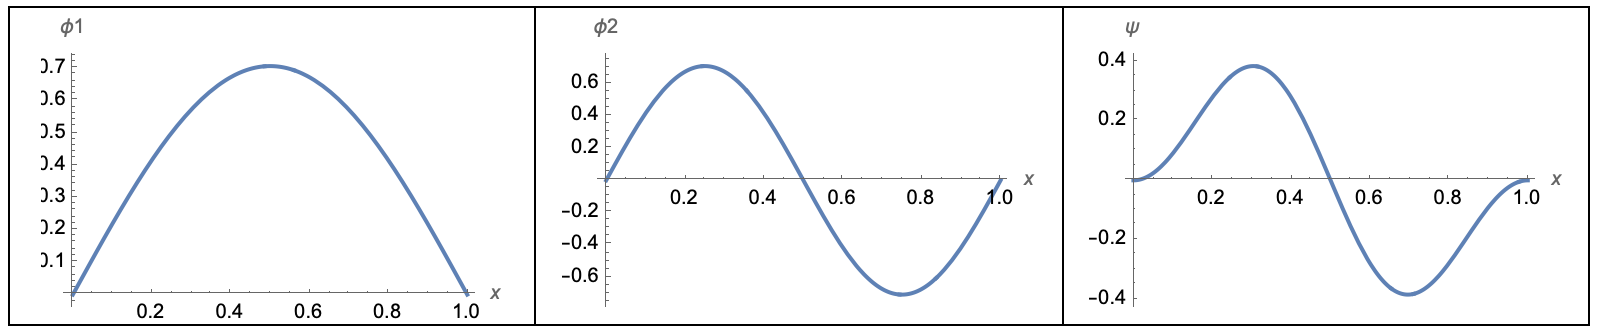
\includegraphics[scale = 0.6]{holestatefunc}	
\centering
\vspace{0.1in}
\caption{Da destra verso sinistra si hanno  le funzioni d'onda $\varphi_1,\varphi_2$ e $\varphi_1\varphi_2$ }
\end{figure}

Nella seguente immagine avremo l'evoluzione temporale del pacchetto di probabilit\`a all'interno della buca infinita di potenziale, procedendo da destra verso sinistra e viceversa. Avremo che in $t = \frac{\pi}{2} \frac{\hbar}{(E_2 - E_1)}$, il coseno in (2.39)  si annulla e la probabilit\`a che la particella si trovi nel centro della buca \`e inferiore a quella che si trovi al lato destro o sinistro della scatola. Come riportato nelle figure centrali. Per $t = \pi \frac{\hbar}{(E_2 -E_1)}$ la probabilit\`a che la particella si trovi al lato sinistro della buca \`e massima.
\begin{figure}[!ht]
\vspace{0.1in}
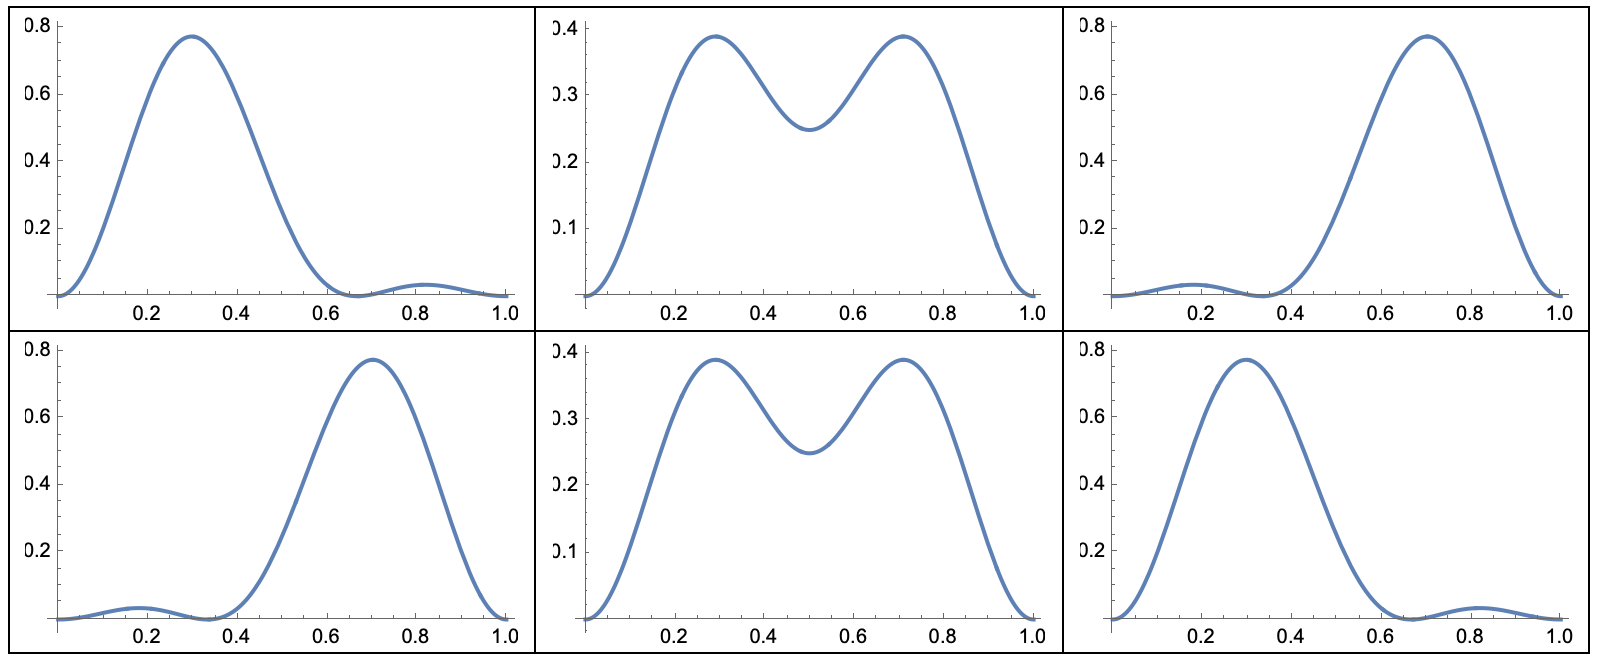
\includegraphics[scale = 0.5]{probevo}	
\centering
\vspace{0.1in}
\end{figure}

In sostanza abbiamo che il pacchetto di probabilit\`a evolve all'interno della buca di potenziale dalle parete infinite, muovendosi avanti e indietro come in figura.

\newpage

\subsection{Esercizio 2: Expanding Box}

Consideriamo una particella confinata in una buca infinita di ampiezza $a$, e nel suo stato fondamentale (\textit{groundstate}), e che istantaneamente si espande raggiungendo un ampiezza $2a$. Determinare la probabilit\`a che la particella resti nello stato fondamentale nel nuovo sistema trasformato.
\begin{figure}[!ht]
\vspace{0.1in}
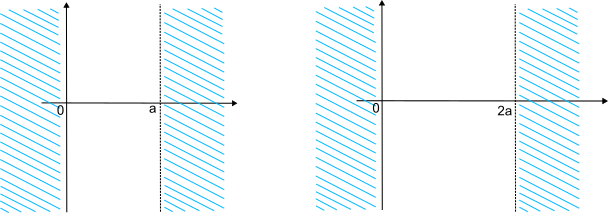
\includegraphics[width = 14cm]{expanding}	
\centering
\end{figure}

Con istantaneamente si intende che la trasformazione avviene cos\`i rapidamente che la particella non ha il tempo di scontare l'informazione, e quindi il suo stato rimane invariato.
\begin{wrapfigure}{l}{0.4\textwidth} % 'r' for right, width of the figure
    \centering
    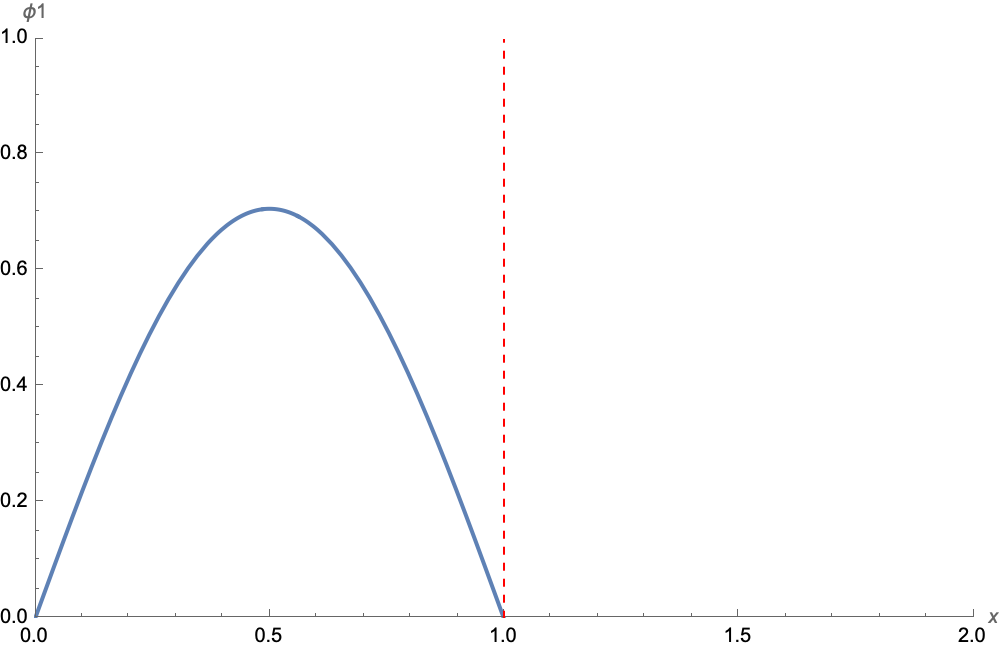
\includegraphics[width=0.4\textwidth]{expstate} % Adjust size and path to image
    \caption{Funzione d'onda allo stato fondamentale per $a=1$.}
\end{wrapfigure}
La funzione d'onda assume l'espressione: 
\begin{equation*}
	\varphi(x) = \left \{ \begin{array}{l}
		 \sqrt{\frac{2}{a}} \sin \left ( \frac{\pi x}{a}\right) \quad 0 <x < a \\[0.5cm]
		 0 \quad a < x <2a
	\end{array}\right.
\end{equation*} 
Raddoppiando la dimensione della buca di potenziale  le autofunzioni della buca iniziale non sono pi\`u le stesse, ma diventano 
\begin{equation*}
	\tilde{\varphi}_n(x) = \sqrt{\frac{2}{2a}}\sin \left (\frac{n\pi x }{2a}\right) = \sqrt{\frac{1}{a}} \sin \left( \frac{n\pi x}{2a}\right) 
\end{equation*}
\newline
I coefficienti delle autofunzioni dello stato iniziale deve essere riscritta rispetto agli elementi della nuova base 
\begin{equation*}
	\varphi(x) = \sum_{n}c_n \tilde{\varphi}_n(x) \quad \text{dove} \quad c_n = \int_0^{2a}dx \; \tilde{\varphi}_n(x) \varphi(x)
\end{equation*}

\begin{figure}[!ht]
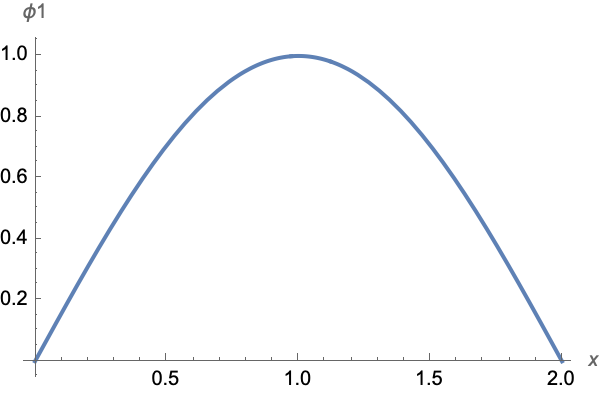
\includegraphics[width = 6cm]{newstate}	
\centering
\caption{Nuovo stato per la buca espansa e a = 2.}
\end{figure}

\newpage 

\begin{proof}
La probabilit\`a che il sistema resti nello stato di partenza \`e data da: 

	\begin{equation*}
		P(\text{fondamentale}) = \left | \int_{0}^{2a}dx \;  \tilde{\varphi_1}(x)\varphi(x) \right |^2 = \left | \int_0^{2a}dx \; \sqrt{\frac{1}{a}}\sin \left(\frac{\pi x}{2a} \right)\sqrt{\frac{2}{a}}\sin \left( \frac{\pi x}{a}\right) \right|^2 = \left| 4\frac{\sqrt{2}}{3\pi}\right|^2
	\end{equation*}
	
\end{proof}
\subsection{Esercizio 3: Rotatore piano}

Consideriamo una particella vincola a muoversi lungo una circonferenza di raggio R. Il moto della particella \`e descritto unicamente dall'angolo $\phi$ e dunque la Hamiltoniana associata \`e data da 
\begin{equation*}
	H = -\frac{\hbar^2}{2I} \frac{d^2}{d\phi^2}
\end{equation*}
dipendendo da un angolo \`e implicito che il problema abbia una sua periodicit\`a $\phi \simeq \phi_0 + 2 \pi$. La trattazione del problemi \`e analoga a quella della buca infinita solo che consideriamo come condizioni al contorno
\begin{equation*}
	\psi(2\pi) = \psi(0) \quad \text{oppure} \quad \psi(\phi+2\pi) = \psi(\phi)
\end{equation*}
che equivale a imporre una certa periodicit\`a nel problema. 

Le autofunzioni e autovalori associati, soluzione dell'equazione di Schr\"odinger
\begin{equation*}
	-\frac{\hbar^2}{2I}\psi_n''(\phi) = E_n\psi(\phi)
\end{equation*}
dove 
\begin{equation*}
	\psi(\phi) = \frac{1}{\sqrt{2\pi}}e^{in\phi} \quad \text{e} \quad E_n = \frac{\hbar^2 n^2}{2I} 
\end{equation*}
Imponendo la condizione di periodicit\`a dobbiamo avere che 
\begin{align*}
	\psi(\phi + 2\pi) = \psi(\phi) \iff & e^{in(\phi + 2\pi)} = e^{in\phi} \\[0.5cm]
	\iff & e^{in 2\pi} = 1 \\[0.5cm]
	\iff & n \in \mathbb{Z}
\end{align*}
Gli stati $\varphi_n(\phi)$ e $ \varphi_{-n}(\phi)$ corrispondono allo stesso livello di energia dato che $E \sim n^2$, l'unica eccezione \`e data da $\varphi_0(\phi)$.
\newline

Utilizzando quanto definito prima, vogliamo determinare l'evoluzione temporale dello stato di partenza dato da 
\begin{equation*}
	\psi(\phi,0) = A \sin^2\phi
\end{equation*}
\newpage

\begin{proof}
	Innanzitutto riscriviamo lo stato iniziale come
	\begin{equation*}
		\psi(0) = A \left( \frac{1-\cos 2\phi}{2} \right) = \frac{A}{2} \left( 1 - \frac{e^{i2\phi} - e^{-i2\phi}}{2}\right)
	\end{equation*} 
riscriviamo lo stato iniziale rispetto alle autofunzioni del rotatore rigido
\begin{equation*}
	\psi(0) = K (2\varphi_0 - \varphi_{2} - \varphi_{-2} )
\end{equation*}
essendo lo spettro della Hamiltoniana discreto, per normalizzare la funzione dobbiamo determinare la costante K, e quindi otteniamo lo stato di partenza 
\begin{equation*}
	\psi(0) = \frac{2\varphi_0 - \varphi_{2} - \varphi_{-2}}{\sqrt{2+1+1}} = \frac{2\varphi_0 - \varphi_{2} - \varphi_{-2}}{\sqrt{6}} 
\end{equation*}
applicando l'operatore di evoluzione temporale $U(t) = e^{- \frac{i}{\hbar}Ht}$ abbiamo che 
\begin{align*}
	\psi(t) = U(t) \psi(0) = & \frac{1}{\sqrt{6}}(2\varphi_0e^{- \frac{i}{\hbar}E_0t} - \varphi_{2}e^{-\frac{i}{\hbar}E_2t} - \varphi_{-2}e^{-\frac{i}{\hbar}E_{-2}t})= \\[0.5cm]
	= & \frac{1}{\sqrt{6}}[2\varphi_0 - e^{-\frac{2 i\hbar^2}{I}t}(\varphi_{2} + \varphi_{-2})] \\[0.5cm]
	= & \frac{1}{\sqrt{3 \pi}}[1 - e^{-\frac{2i \hbar^2}{I}t}\cos(2\phi)]
\end{align*}

\end{proof}

\subsection{Esercizio 4: Buca infinita in 3D}

L'equazione di schr\"odinger per un sistema di dimensione tre \`e data da
\begin{equation*}
	- \frac{\hbar^2}{2m	} \left ( \frac{d^2}{dx^2} + \frac{d^2}{dy^2} + \frac{d^2}{dz^2}\right)\psi(x,y,z) + V(x,y,z)\psi(x,y,z) = E\psi(x,y,z)
\end{equation*}
dove possiamo considerare il caso in cui il potenziale pu\`o essere fattorizzato in tre termini dipendenti dalle singole coordinate
\begin{equation*}
	V(x,y,z) = K(x) + W(y) +T(z)
\end{equation*}
in questo modo l'equazione di Schr\"odinger diventa
\begin{equation*}
	\left (-\frac{\hbar^2}{2m} \frac{d}{dx^2} +K(x)\right)\psi  + \left( -\frac{\hbar^2}{2m} \frac{d^2}{dy^2} +W(y)\right)\psi + \left( -\frac{\hbar^2}{2m}\frac{d^2}{dz^2} +T(z)\right)\psi = (E_x+E_y +E_z)\psi
\end{equation*}
che possiamo vedere come la somma di tre Hamiltoniane rispetto alla singola coordinata
\begin{equation*}
	H = H_x + H_y + H_z
\end{equation*}

questo equivale ad avere un sistema di tre equazioni differenziali ordinarie del secondo ordine
\newpage 
\begin{equation*}
	\left \{ \begin{array}{l}
		H_x \psi_1(x) = E_x \psi_1(x)\\[0.3cm]
		H_y \psi_2(y) = E_y\psi_2(y) \\[0.3cm]
		H_z \psi_3(z) = E_z \psi_3(z)
	\end{array}\right. 
\end{equation*}
dove la soluzione dell'equazione di Schr\"odinger definita inizialmente pu\`o essere scritta come prodotto di tre funzioni rispetto alle singole coordinate
\begin{equation*}
	\psi(x,y,z) = \psi_1(x)\psi_2(y)\psi_3(z) \quad \text{e} \quad E = E_x + E_y + E_z
\end{equation*}
Se prendiamo una buca infinita in tre dimensioni,con larghezza $\bold{a}$, il potenziale associato \`e dato da 
\begin{wrapfigure}{r}{0.4\textwidth} % {r} for right, {0.4\textwidth} for width
    \centering
    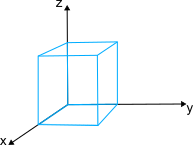
\includegraphics[width=0.38\textwidth]{cube} % Replace with your image
\end{wrapfigure}

\begin{equation*}
	V(x,y,z) = \left \{ \begin{array}{l}
		0 \quad \text{per} \quad x \in [0,a_1]; y\in [0,a_2]; z \in [0,a_3] \\[0.3cm]
		\infty \quad \text{altrimenti}
	\end{array}\right.
\end{equation*}


\noindent Le autofunzioni sono tutti i possibili prodotto della autofunzioni della buca infinita monodimensionale
\begin{align*}
\psi_{n_1}(x) = \sqrt{\frac{2}{a_1} } \sin \left( \frac{n_1 \pi x}{a_1} \right)\\[0.5cm]
\psi_{n_2}(y) = \sqrt{\frac{2}{a_2}} \sin \left ( \frac{n_2\pi y}{a_2}\right) \\[0.5cm]
\psi_{n_3}(z) = \sqrt{\frac{2}{a_3}}\sin \left( \frac{n_3 \pi x}{a_3}\right)
\end{align*}

In notazione di Dirac indichiamo lo stato $|\psi(x,y,z) \rangle = |n_1 \; n_2 \; n_3 \rangle  $. L'auto energia associata \`e espressa come 
\begin{equation*}
	E = \frac{\hbar^2 \pi^2 n_1^2}{2ma_1^2} + \frac{\hbar^2 \pi^2 n_2^2}{2ma_2^2} + \frac{\hbar^2 \pi^2 n_3^2}{2ma_3^2}
\end{equation*}

\subsection{Esercizio 5: Buca infinita in 2D}

Data una particella confinata nel  seguente potenziale 
\begin{equation*}
	V(x,y) = \left \{ \begin{array}{l}
		0 \quad \text{per} \quad x \in [0,a]; y \in [0,a]\\[0.3cm]
		\infty \quad \text{altrimenti}
	\end{array}\right.
\end{equation*}
la cui evoluzione dinamica \`e data dalla Hamiltoniana 
\begin{equation*}
	H = - \frac{\hbar^2}{2m} \left (\frac{d^2}{dx^2} +\frac{d^2}{dy^2}\right) + V(x,y)  
\end{equation*}
\newpage
e che si trova nel seguente stato iniziale 
\begin{equation*}
	\psi = N \cos \left( \frac{\pi x}{a}\right) \cos\left( \frac{\pi y}{a}\right) \sin \left( \frac{2 \pi x}{a}\right)\sin \left( \frac{2 \pi y}{a}\right)
\end{equation*}
determinare: 
\begin{enumerate}
	\item La probabilit\`a rispetto ai livelli di energia dello stato iniziale, il valore di $\langle E \rangle $ e la probabilit\`a per $E_x$.
	\item Se dopo una misurazione si determina che $E_x = \frac{\pi^2 \hbar^2}{2ma^2}$, qual \`e la probabilit\`a che si misuri $E = E_y$ ? 
\end{enumerate}

\begin{proof}
	1) Sappiamo che le autofunzioni soluzione dell'equazione di Schr\"odinger sono 
	\begin{equation*}
		|nm \rangle = \sqrt{\frac{2}{a}} \sin\left(\frac{n\pi x }{a} \right)\sqrt{\frac{2}{a}}\sin \left( \frac{m \pi y}{a}\right)  \quad n,m \in \mathbb{Z}
	\end{equation*}
	e gli autovalori associati sono dati da 
	\begin{equation*}
		E_{nm} = \frac{\hbar^2 \pi^2 n^2}{2\mu a} + \frac{\hbar^2 \pi ^2 m^2}{2 \mu a} \quad n,m \in \mathbb{Z}
	\end{equation*}
Scriviamo lo stato di partenza rispetto alla base formata dalle funzioni $|nm \rangle$
\begin{equation*}
	|\psi\rangle = \frac{|11 \rangle  + |13\rangle + |31\rangle + |33 \rangle }{\sqrt{4}} 
\end{equation*}
le autofunzioni associate sono date dai valori
\begin{equation*}
	E_{11} = \frac{\hbar^2 \pi ^2}{\mu a^2} \quad;\quad  E_{13} = E_{31}=\frac{5\hbar^2 \pi ^2}{\mu a^2}\quad ; \quad E_{33} = \frac{9\hbar^2 \pi^2}{\mu  a^2}
\end{equation*}
La probabilit\`a che la particella si trovi eni diversi stati dell'energia \`e data da 
\begin{equation*}
	P(E=E_{11}) = \frac{1}{4} \quad ; \quad P(E=E{31}=E_{13}) = \frac{1}{4} + \frac{1}{4} = \frac{1}{2} \quad \; \quad P(E=E_{33}) = \frac{1}{4}
\end{equation*}
Il valore medio dell'energia \`e dato da 
\begin{equation*}
	\langle E \rangle = \sum_{n}E_{n}P(E_n) = \frac{1}{4}E_{11} + \frac{1}{2}E_{12} +\frac{1}{4}E_{33} = \frac{5 \hbar^2 \pi^2}{\mu a^2}
\end{equation*}
Infine consideriamo solo i contirbuiti all'energia cinetica rispetto alla coordinata $x$, si ha che 
\begin{align*}
	P \left (E_x = \frac{\hbar^2 \pi^2}{2 \mu a^2}\right ) = \frac{1}{4} + \frac{1}{4} = \frac{1}{2} \\[0.5cm]
	P \left (E_x = \frac{9 \hbar^2 \pi^2}{2\mu a^2}\right )  = \frac{1}{4} + \frac{1}{4} = \frac{1}{2}
\end{align*}
\newpage

2) Dopo aver determinato la probabilit\`a rispetto ad $E_x = \frac{\hbar^2 \pi^2}{2 \mu a^2} $ vogliamo sapere come cambia la probabilit\`a rispetto ad $E_y$.  Dopo aver effettuato una misurazione si ha il collasso della funzione d'onda, dunque la probabilit\`a diventa massima rispetto allo stato osservato, che nel nostro caso \`e dato da 
\begin{equation*}
	|\psi \rangle = \frac{|11 \rangle + |13 \rangle }{\sqrt{2}}
\end{equation*}
La probabilit\`a rispetto ad $y$ assume i seguenti risultati
\begin{align*}
	P \left (E_x = \frac{\hbar^2 \pi^2}{2 \mu a^2}\right ) = ||11\rangle|^2 = \frac{1}{2} \\[0.3cm]
		P \left (E_x = \frac{9 \hbar^2 \pi^2}{2\mu a^2}\right )  = ||13\rangle |^2 = \frac{1}{2}
\end{align*}

\end{proof}

\subsection{Esercizio 6}

Consideriamo un sistema definito su uno spazio di Hilbert $\mathcal{E} = \mathbb{C}^3$, la cui dinamica \`e descritta dalla Hamiltoniana
\begin{equation*}
	H = \hbar \omega_0\left [ \begin{array}{ccc}
		1 & 0 & 0\\
		0 & -1 & 0 \\
		0 & 0 & -1
	\end{array}\right]
\end{equation*} 
dove $\omega_0 \in \mathbb{R}$. Inoltre \`e presente una grandezza fisica osservabile B , il cui operatore associato \`e definito nel seguente modo
\begin{equation*}
	B = b\left [ \begin{array}{ccc}
		1 & 0 & 0\\
		0 & 0 & 1 \\
		0 & 1 & 0
	\end{array}\right]
\end{equation*}
per $b \in \mathbb{R}$. Risolvere i seguenti punti:
\begin{enumerate}
	\item Controllare se $H$ e $B$ sono operatori autoaggiunti.
	\item Determinare una base di autovettori comuni.
	\item Chi tra i seguenti insiemi $\{H\}$,$\{B\}$,$\{B,H\}$ e $\{H^2,B\}$ \`e un sistema di osservabili compatibili completo ? 
\end{enumerate}

\begin{proof}
	1) Una operatore \`e autoaggiunto se $H = H^\dag $ dove $H^\dag = (H^T)^*$, siccome la matrice H \`e diagonale ed \`e costituista da valori reali abbiamo che $H^\dag = H$ e quindi possiamo concludere che la Hamiltoniana del sistema sia un operatore autoaggiunto. Nel caso dell'operatore $\hat{B}$ abbiamo che $B^T = B$ ed \`e anch`esso costituito da valori reali dunque $B^\dag =B$.
	\newline
	
	\noindent 2)Una base comune tra due operatori esiste se e soltanto se questi commutano tra di loro
	\begin{equation*}
		[H,B] = HB -BH = 0
	\end{equation*}
	e quindi l'osservabile B \`e una costante del moto.
	Osserviamo che gli autovettori e autovalori della matrice H sono dati da
	\begin{align*}
	 &\bold{e}_{1} = \left [ \begin{array}{c}
	 	1 \\ 0 \\ 0
	 \end{array}\right] \longrightarrow \lambda_1 = \hbar\omega_0\\[0.5cm]
	  &\bold{e}_{2} = \left [ \begin{array}{c}
	 	0 \\ 1 \\ 0
	 \end{array}\right] \longrightarrow \lambda_2 = -\hbar\omega_0\\[0.5cm]
	  &\bold{e}_{3} = \left [ \begin{array}{c}
	 	0 \\ 0 \\ 1
	 \end{array}\right] \longrightarrow \lambda_3ß = -\hbar\omega_0
	\end{align*}
	Dato che abbiamo degenerazione rispetto agli autovalori, avremo che i vettori che possono essere espressi come
	\begin{equation*}
		\bold{v} = \alpha \bold{e}_2 + \beta \bold{e}_3
	\end{equation*}
	sono autovettori di H con autovalore $\lambda = -\hbar \omega_0$.
	
	Calcoliamo gli autovettori dell'operatore B, osserviamo gi\`a che dalla forma matriciale di tale operatore il vettore $\bold{e}_1$ \`e autovettore di B con autovalore $b$. Per determinare gli altri autovettori calcoliamo le radici associate al polinomio caratteristico della sottomatrice $2 \times 2$ associata a B:
	\begin{equation*}
		P(\lambda) = \text{det} \left [ \begin{array}{cc}
		-\lambda & 1 \\ 1 & -\lambda   
		\end{array} \right ] = \lambda^2-1 = 0
	\end{equation*}
	che ha come radici $\lambda = \pm 1$. Gli autovettori associati sono dati da 
	\begin{align*}
		&\left [ \begin{array}{cc}
		-1 & 1 \\ 1 & -1   
		\end{array} \right ] \left [\begin{array}{c} 
			a \\ b
		\end{array}\right ] = \left [\begin{array}{c} 
			0 \\ 0
		\end{array}\right ] \Rightarrow U_2 = \frac{1}{\sqrt{2}}\left [\begin{array}{c} 
			1 \\ 1
		\end{array}\right ] \rightarrow \lambda =1 \\[0.5cm]
		& \left [ \begin{array}{cc}
		1 & 1 \\ 1 & 1   
		\end{array} \right ] \left [\begin{array}{c} 
			a \\ b
		\end{array}\right ] = \left [\begin{array}{c} 
			0 \\ 0
		\end{array}\right ] \Rightarrow U_3 = \frac{1}{\sqrt{2}}\left [\begin{array}{c} 
			1 \\ -1
		\end{array}\right ] \rightarrow \lambda = -1
	\end{align*}
	che nel caso dell'operatore B hanno autovalore $-b$. Tali autovettori di B sono anche autovettori di H dato che possono essere scritti come combinazione lineare di $\bold{e}_2$ e $\bold{e}_3$. Posto $U_{1} = \bold{e}_{1}$, una base comune ai due operatori \`e data da $\{U_1,U_2,U_3\}$. Dove
	\begin{equation*}
		U_2 = \frac{1}{\sqrt{2}}\left [ \begin{array}{c}
			0 \\ 1 \\ 1
		\end{array}\right] \quad ; \quad U_3 = \frac{1}{\sqrt{2}} \left [ \begin{array}{c}
			0 \\ 1 \\ -1
		\end{array}\right] 
	\end{equation*}
\noindent 3) Compatibile vuol dire che gli operatori presenti nell'insieme commutano tra di loro, mentre con completo si intende che effetuata una misura questa \`e univocamente determinata. Nel nostro caso abbiamo tre vettori $\{U_1,U_2,U_3\}$ e quindi abbiamo tre possibili risultati delle misure.

Consideriamo l'insieme $\{H \}$ e $\{B\}$ tali insiemi sicuramente sono compatibili, ma non completi dato che se effettuiamo una misura e otteniamo come risultato $-\hbar\omega_0$ o $b$, non sappiamo se l'autostato associato \`e dato da $U_2$ o $U_3$ o una loro combinazione lineare, oppure $U_1$ o $U_2$ o una loro combinazione lineare.

L'insieme $\{H^2 ,B \}$ analogamente a quanto discusso prima \`e si formato da operatori completi, ma non compatibili dato che per $b$ o $\hbar^2 \omega_0^2$ si ha degenerazione rispetto agli autostati.

L'ultimo caso da analizzare \`e dato dall'insieme $\{H,B\}$ che risulta essere un sistema completo per quanto verificato al punto 1) e inoltre  \`e completo poich\`e rispetto alla base comuni di autostati $\{U_1,U_2,U_3\}$, abbiamo che le coppie simultanee possibili sono tutte distinte ed associabili a un solo autostato.

\end{proof}

\subsection{Esercizio 7}

Consideriamo un sistema definito su uno spazio di Hilbert $\mathcal{E} = \mathbb{C}^3$, la cui dinamica \`e descritta dalla Hamiltoniana
\begin{equation*}
	H = \hbar \omega_0\left [ \begin{array}{ccc}
		1 & 0 & 0\\
		0 & 2 & 0 \\
		0 & 0 & 2
	\end{array}\right]
\end{equation*} 
dove $\omega_0 \in \mathbb{R}$. Inoltre sono presenti le grandezze fisiche osservabili A e  B , il cui operatore associato \`e definito nel seguente modo
\begin{equation*}
A = a\left [ \begin{array}{ccc}
		1 & 0 & 0\\
		0 & 0 & 1 \\
		0 & 1 & 0
	\end{array}\right] 
	\quad \quad B = b\left [ \begin{array}{ccc}
		0 & 1 & 0\\
		1 & 0 & 0 \\
		0 & 0 & 1
	\end{array}\right] 
\end{equation*}
Inoltre lo stato iniziale del sistema \`e 
\begin{equation*}
	|\psi(0) \rangle = \left[ \begin{array}{c}
		\frac{1}{\sqrt{2}} \\ \frac{1}{2} \\ \frac{1}{2}
	\end{array}\right ]
\end{equation*}
Determinare:
\begin{enumerate}
	\item La probabilit\`a per i livelli di energia E possibili, il valore medio di $\langle E \rangle $, la sua varianza $\Delta E$ al tempo $t=0$.
	\item La probabilit\`a e valori medi per gli osservabili A e B al tempo generico $t$.
\end{enumerate}

\begin{proof}
	1) Gli autovalori associati alla Hamiltoniana sono dati dagli elementi della base canonica $\{\bold{e}_{1},\bold{e}_{2},\bold{e}_3\}$ con i corrispettivi autovalori $\{\hbar \omega_0,2\hbar \omega_0,2\hbar \omega_0 \}$. Riscriviamo lo stato inzile rispetto a tale base 
	\begin{equation*}
		|\psi(0) \rangle = \frac{1}{\sqrt{2}}\bold{e}_1 + \frac{1}{2} \bold{e}_2 + \frac{1}{2} \bold{e}_{3}
	\end{equation*}
Calcoliamo la probabilit\`a che il sistema si trovi negli stati energetici definiti dalla 
Hamiltoniana
\begin{equation*}
P(E = \hbar\omega_0) = \left | \frac{1}{\sqrt{2}} \right |^2 = \frac{1}{2} \quad ; \quad P(E = 2 \hbar \omega_0) = \frac{1}{4} + \frac{1}{4} = \frac{1}{2} 	
\end{equation*}
Il valore medio dell'energia \`e dato da
\begin{equation*}
	\langle E \rangle = \sum_{n} E_n P(E=E_n) = \hbar \omega_0 \frac{1}{2} + 2 \hbar \omega_0 \frac{1}{2} = \frac{3}{2}\hbar \omega_0
\end{equation*}
la deviazione standard associata viene calcolata nel seguente modo
\begin{equation*}
	\Delta E = \sqrt{\langle E^2 \rangle - \langle E \rangle ^2} 
\end{equation*}
calcoliamo il termine
\begin{equation*}
	\langle E^2 \rangle = \sum_{n}E_n^2 P(E_n) = \hbar^2 \omega_0^2 \frac{1}{2}  + \frac{1}{2}4 \hbar^2 \omega_0^2 = \frac{5}{2}\hbar^2 \omega_0^2
\end{equation*}
quindi l'incertezza sulla misura dell'energia \`e data da 
\begin{equation*}
	\Delta E = \sqrt{\frac{5}{2} \hbar^2 \omega_0^2 - \frac{9}{4} \hbar^2 \omega_0^2} = \frac{1}{2}\hbar \omega_0
\end{equation*}
2) Per determinare l'evoluzione temporale dello stato applichiamo l'operatore di evoluzione temporale allo stato iniziale $|\psi(0) \rangle $, ovvero
\begin{equation*}
	|\psi \rangle = U(t)|\psi(0) \rangle = e^{- \frac{i}{\hbar}Ht}|\psi(0)\rangle 
\end{equation*}
ottenendo
\begin{equation*}
	|\psi(t) \rangle = \frac{1}{\sqrt{2}} e^{-i\omega_0 t}\bold{e}_{1}+ \frac{1}{2} e^{-2i\omega_0t}\bold{e}_{2} + \frac{1}{2}e^{-2i \omega_0 t}\bold{e}_{3}
\end{equation*}
Procediamo con il calcolare gli autovettori e autovalori dell'operatore $\hat{A}$. Determinando
\begin{equation*}
	U_1 = \bold{e}_{1} \rightarrow \lambda = a \quad ; \quad U_2 = \frac{1}{\sqrt{2}}\left [ \begin{array}{c}
			0 \\ 1 \\ 1
		\end{array}\right]  \rightarrow \lambda = a \quad ; \quad U_3 = \frac{1}{\sqrt{2}}\left [ \begin{array}{c}
			0 \\ 1 \\ -1 
		\end{array}\right]\rightarrow \lambda = -a 
\end{equation*}

La probabilit\`a associata alle due misure possibili dell'osservabile $A$ \`e data da 
\begin{equation*}
	P(A = -a) = |\langle U_3 | \psi(t) \rangle |^2 = \left |\frac{1}{\sqrt{2}} [0 \; 1 \; -1]^* \cdot \left [ \begin{array}{c}
		\frac{e^{-i \omega_0t}}{\sqrt{2}} \\ \frac{e^{-i2 \omega_0 t}}{2} \\ \frac{e^{-i2 \omega_0 t}}{2}
	\end{array}\right] \right|^2 = 0
\end{equation*}	
dato che la somma delle probabilit\`a degli stati deve essere uguale a uno, possiamo concludere che $P(A = a) =\frac{1}{2} + \frac{1}{2} = 1$.
Infinite calcoliamo il valore medio di A
\newpage

\begin{equation*}
	\langle A \rangle = \sum_{n}AP(A) = aP(A=a)-aP(A =-a) =a
\end{equation*}
in alternativa possiamo procedere al calcolo considerando
\begin{equation*}
	\langle \psi(t)|A|\psi(t) \rangle = \left [ \frac{e^{-i \omega_0t}}{\sqrt{2}} \\ \frac{e^{-i2 \omega_0 t}}{2} \\ \frac{e^{-i2 \omega_0 t}}{2}\right] a \left [ \begin{array}{ccc}
		1 & 0 & 0\\
		0 & 0 & 1 \\
		0 & 1 & 0
	\end{array}\right] \left [ \begin{array}{c}
		\frac{e^{-i \omega_0t}}{\sqrt{2}} \\ \frac{e^{-i2 \omega_0 t}}{2} \\ \frac{e^{-i2 \omega_0 t}}{2}
	\end{array}\right] = a
\end{equation*}
Analoga discussione viene fatta per le grandezza richieste relative all'osservabile B.

\end{proof}

\subsection{Esercizio 8: Notazione di Heisenberg}

Consideriamo una particella soggetta al potenziale $V(x) = - fx$. Qual \`e il valore di $\Delta p(t) ?$

\begin{proof}
	Per rispondere alla domanda usiamo la notazione di Heisenberg rispetto a cui vale la relazione 
	\begin{equation*}
		\frac{d}{dt}A_H = \frac{\partial A_H}{\partial t} + \frac{1}{i \hbar}[A_H,H]
	\end{equation*}
	dove definiamo $A_H$, ovvero la rappresentazione di un generico operatore A nella notazione di Heinsenberg, nel seguente modo
	\begin{equation*}
		\langle A \rangle = \langle \psi(t) |A|\psi(t) \rangle = \langle \psi(t_0)|e^{\frac{i}{\hbar}H(t-t_0)}Ae^{\frac{i}{\hbar}H(t-t_0)}|\psi(0)\rangle   = \langle \psi(0)|A_H|\psi(0) \rangle 
	\end{equation*}
e quindi 
\begin{equation*}
	A_H = e^{\frac{i}{\hbar}H(t-t_0)}Ae^{\frac{i}{\hbar}H(t-t_0)}
\end{equation*}
Utilizzando tale notazione gli operatori momento e posizione definiscono il seguente sistema di equazioni
\begin{equation*}
	\left \{ \begin{array}{l}
		\frac{d}{dt}x_H = \frac{p_H}{m} \\[0.3cm]
	  \frac{d p_H}{dt} = -V'(x_H) = f
	\end{array}\right.
\end{equation*}	
ottenendo la seguente legge orarie
\begin{equation*}
x_H = \frac{f}{2m}t^2 + \frac{p_0}{m}t +x_0
\end{equation*}
che abbiamo ottenuto calcolando
\begin{equation*}
	p_H(t) = ft + p_0
\end{equation*}
e sostituendolo nella quadratura della prima equazione. Utilizzando tale risultato intermedio procediamo a calcolare l'incertezza sui momenti, dove
\begin{equation*}
	\langle p_h \rangle  = \langle \psi(0) | p_h |\psi(0) \rangle = ft + \langle p_0\rangle = \langle p \rangle  
\end{equation*} 
\newpage 


si ha che l'uguaglianza coincide con quella nella notazione di Dirac. Da qui in poi si procede come negli esercizi precedenti, calcolando il risultato intermedio
\begin{equation*}
	\langle p^2 \rangle = \langle (ft+p_0)^2 \rangle = f^2t^2 + 2ft \langle p_0 \rangle + \langle p_0 \rangle^2
\end{equation*}
Infine 
\begin{equation*}
	\Delta p^2 = \langle p^2 \rangle - \langle p \rangle ^2 = f^2t^2 + 2ft \langle p_0 \rangle + \langle p_0^2\rangle - f^2t^2-2ft\langle p_0 \rangle - \langle p_0 \rangle^2 = \langle p_0^2 \rangle - \langle p_0 \rangle^2 = \Delta p^2(t=0) 
\end{equation*}
La varianza dell'operatore p resta costante nel tempo.
\end{proof}

\setcounter{chapter}{2}
\chapter{Sistemi Semplici}

\section{Momento Angolare Orbitale}

In meccanica classica abbiamo visto come per alcuni sistemi il \textit{momento angolare} fosse una variabile ciclica del moto. Come grandezza questa \`e sempre definita rispetto ad un polo O rispetto al quale viene misurata e nel caso in cui si conservi 
\begin{equation*}
	\frac{d \bold{L}}{d t} = 0
\end{equation*}

la sua conservazione ci fornisce l'importante informazione che il moto \`e vincolato ad un piano contenete O e il punto di misurazione P. In meccanica quantistica possiamo definire le medesime propriet\`a, solo che come abbiamo visto nel caso di posizione e momento, dobbiamo costruire un operatore lineare rispetto all'osservabile $\bold{L}$. Per farlo passiamo dalla sua espressione classica 
\begin{equation*}
	\bold{L} = \bold{r} \times \bold{p}
\end{equation*}
che utilizzando le definizione di operatore di $\bold{r}$ e $\bold{p}$ assume come forma di operatore
\begin{equation}
	\bold{L} = i\hbar \bold{x} \times \nabla 
\end{equation}
l'operatore cos\`i ottenuto \`e auto-aggiunto dato che lo sono anche $\bold{r}$ e $\bold{p}$.
Facendo il prodotto vettoriale dell'operatore del  momento angolare orbitale otteniamo un vettore le cui componenti sono uguali a
\begin{equation*}
	\left \{ \begin{array}{l}
		L_x = yp_z - z p_y \\
		L_y = zp_x - x p_z \\ 
		L_z = xp_y - yp_x
	\end{array} \right.
\end{equation*}
Dato che conosciamo le relazioni di commutazione per $\bold{r}$ e $\bold{p}$, dove $[r_i,p_j] = i \hbar \delta_{ij}$, dove le componenti commutano solo per $i \neq j$, possiamo calcolare la commutazione tra le componenti del momento. 
\begin{equation*}
	\left \{ \begin{aligned}[]
 	 &[L_y,L_z] = i \hbar L_x \\ 
 	 &[L_z,L_x] = i \hbar L_y \\ 
 	 &[L_x,L_y] = i \hbar L_z \\
 \end{aligned}\right.
\end{equation*}

Dal un punto di vista fisico, questo vuol dire che una particella, descritta da un punto di vista quantistico, non pu\`o avere un momento angolare ben definito in tutte e tre le direzioni contemporaneamente. Per esempio se conosciamo il momento angolare $L_x$, allora necessariamente avremo incertezza per il momento angolare nelle altre due direzioni.

\subsubsection{Notazione compatta del commutatore}

Un moto per esprimere in forma compatta il commutatore delle componenti del momento angolare \`e data dall'utilizzo del \textit{tensore di Levi-Civita}. In tre dimensioni viene indicato come  $\epsilon_{ijk}$ ed \`e definito come
\begin{equation*}
	\epsilon_{ijk} = \left \{ \begin{array}{l}
		+ 1 \quad \text{se (i,j,k) \`e una permutazione pari di (1,2,3)}\\
		-1 \quad \text{se (i,j,k) \`e una permutazione dispari di (1,2,3)}\\
		0 \quad \text{se i = j = k} \; \text{o se almeno due indici sono uguali}
	\end{array}\right.
\end{equation*}
Una terna di elementi che permutano tra loro \`e data dagli elementi del gruppo $S_3$ che pu\`o essere visto come l'insieme delle simmetrie e rotazioni di un triangolo. Il gruppo possiede i seguenti elementi definiti in notazione ciclica
\begin{equation*}
	S_3 = \big \{ id,(1)(23),(2)(13),(3)(12),(231),(321)\big \} 
\end{equation*}
dove per esempio con l'elemento 
\begin{equation*}
	(1)(23) = \left ( \begin{array}{ccc}
		1 & 2 & 3 \\
		1 & 3 & 2
	\end{array}\right ) 
	\iff 
	\begin{array}{l}
		1 \to 1 \\
		2 \to 3 \\ 
		3 \to 2 \\
	\end{array}
\end{equation*}
Ogni 3-ciclo formato da $(a_1 \; a_2 \; a_3)$ possiamo riscriverlo come prodotto di 2-cicli
\begin{equation*}
	(a_1 \; a_2 \; a_3) = (a_1a_3)(a_1a_2)
\end{equation*}
che sono disgiunti tra loro, e coincidono con delle trasposizioni. Una permutazione \`e detta pari o dispari a seconda che sia ottenibili come prodotto di un numero pari o dispari di trasposizioni.
Dunque nel caso del gruppo $S_3$ si ha che le permutazioni 
\begin{equation*}
	\begin{aligned}
		& (23),(13),(13) \quad \text{sono permutazioni di segno dispari} & \\ 
		& id,(132),(231) \quad \text{sono permutazioni di segno pari}
	\end{aligned}
\end{equation*}
Utilizzando questi risultati possiamo definire in generale il commutatore del momento angolare come 
\begin{equation}
	[L_i,L_j] = i\hbar \epsilon_{ijk}L_k
\end{equation}
Per esempio se associato la terna (x,y,z) a (1,2,3) avremo che fissato il momento lungo $\hat{z}$ si ha che 
\begin{equation*}
	[L_x,L_y] = i\hbar\epsilon_{123}L_{z} = i\hbar L_z
\end{equation*}
Se scambiamo di ordine i momenti 
\begin{equation*}
	[L_y,L_x] = i \hbar \epsilon_{213}L_{z}  = -i\hbar L_{z}
\end{equation*}
questo ci suggerisce che il tensore di Levi-Civita gode della propriet\`a di antisimmetria.

\subsection{Momento Angolare Totale}

Possiamo anche definire l'intensit\`a del vettore momento angolare. In questo caso \`e pi\`u utile considerare $\bold{L}^2$ invece di $|\bold{L}|$. Tale grandezza \`e associata all'operatore di \textit{momento angolare totale}
\begin{equation*}
	\hat{\bold{L}}^2 = \hat{L}_{x}^2 + \hat{L}_{y}^2+ \hat{L}_{z}^2
\end{equation*}
Anche questo \`e un operatore auto-aggiunto e commuta con tutte le componenti $\hat{L}_{i}$
\begin{equation*}
	[\hat{\bold{L}}^2,L_i] = 0
\end{equation*}
Come definito nel paragrafo precedente, in meccanica quantistica non possiamo misurare simultaneamente il valore di tutte le componenti del momento angolare nelle varie direzioni. Per\`o per una stato del sistema che possiede un determinato momento angolare totale (e quindi vuol dire che \`e autostato dell'operatore $\hat{\bold{L}}^2$) e una misura del momento angolare lungo una direzione, si ha che i due operatori commutano tra loro e quindi hanno una base di autofunzioni in comune, di conseguenza l'autostato di $\bold{\hat{L}}^2$ \`e anche autostato di $\bold{\hat{L}}_i$. 
\\
In sostanza in meccanica quantistica per quanto riguarda l'operatore del momento angolare possiamo misurare simultaneamente e con precisione magnitudo e direzione del momento angolare rispetto ad un asse del sistema di riferimento.
\begin{equation}
	\left \{\begin{array}{l}
		\bold{\hat{L}}^2 \psi = L^2\psi \\
		\hat{L}_z\psi = L \psi
	\end{array}\right.
\end{equation}  
si dimostra che gli autovalori comuni a $\bold{\hat{L}}^2$ e $\hat{L}_z$  che indichiamo come $\mid L \;m \rangle$ possono assumere solo valori discreti, ovvero
\begin{equation*}
	\begin{aligned}
		& l = 0,1,2,.... & \\
		& m \in \mathbb{Z} \quad \text{dove} \; |m| < l
	\end{aligned}
\end{equation*}
e assumono la forma
\begin{equation*}
	\begin{aligned}
		& L^2 = \hbar^2 l(l+1) & \\
		& L = \hbar m
	\end{aligned}
\end{equation*}
tale condizione ci definisce la \textit{quantizzazione del momento angolare}. "l" rappresenta la lunghezza del vettore momento angolare (\textit{Numero quantistico del momento angolare totale}) ed "m" ci dice qual \`e la proiezione rispetto ad un asse di riferimento ( \textit{momento angolare azimutale}).

\subsubsection{Esempio}

Consideriamo il caso in cui $l = 2 $.
\begin{equation*}
	\begin{array}{ccc}
		m & L^2 & L_z  \\
	\hline
	-2 & 6\hbar^2 & -2\hbar \\
	-1 & 6\hbar^2 & -\hbar \\
	0 & 6\hbar^2 &  0 \\
	1 & 6\hbar^2 & \hbar \\
	-2 & 6\hbar^2 & 2 \hbar
	\end{array}
\end{equation*}
\begin{figure}[!ht]
\vspace{0.1in}
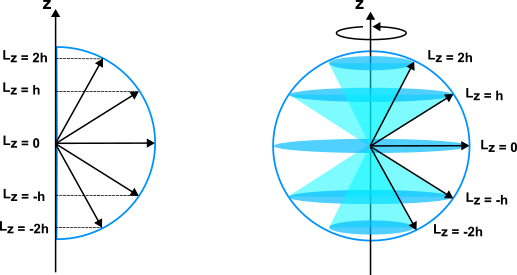
\includegraphics[width = 12cm]{angular_momentum}	
\centering
\vspace{0.1in}
\end{figure}

Si noti come in figura il vettore del momento angolare $\bold{L}$ non punti mai nella direzione $\hat{z}$ dato che $L_z$ deve essere  pi\`u piccola dell'intensit\`a di $\bold{L}$. Tale risultato \`e conseguenza del principo d'indeterminazione del momento angolare che ci dice che non possiamo conoscere con precisione pi\`u di una componente del momento angolare.
\\
Da un punto di vista tridimensionale come nella seconda figura abbiamo che $\bold{L}$ precede attorno all'asse z, definendo un cono con angolo $\theta$ dato da 
\begin{equation*}
	cos\theta = \frac{L_z}{L} = \frac{m_l}{\sqrt{l(l+1)}}
\end{equation*}
che definisce la quantizzazione dello spazio rispetto ad $\bold{L}$.

\subsection{Funzioni armoniche sferiche}

In coordinate cartesiane le componenti dell'operatore di momento orbitale sono date da 
\begin{equation*}
	\begin{aligned}
		L_x = \frac{\hbar}{i} \left ( y\frac{\partial}{\partial z} - z \frac{\partial}{\partial y}\right ) \\[0.3cm]
		L_y = \frac{\hbar}{i} \left ( z \frac{\partial}{\partial x}- x \frac{\partial}{\partial z}\right )\\[0.3cm]
		L_z =  \frac{\hbar}{i} \left ( x \frac{\partial}{\partial y} - y \frac{\partial}{\partial x}\right )
	\end{aligned}
\end{equation*}
Essendo il momento orbitale un operatore differenziale \`e comodo esprimerlo in coordinate sferiche dato che come vedremo l'operatore momento angolare agisce sulle variabili angolari $\theta$ e $\varphi$. Utilizzando il cambio di variabili riscriviamo le componenti come
\begin{equation*}
	\begin{aligned}
L_x & =i \hbar\left(\sin \varphi \frac{\partial}{\partial \theta}+\frac{\cos \varphi}{\tan \theta} \frac{\partial}{\partial \varphi}\right) \\
L_y & =i \hbar\left(-\cos \varphi \frac{\partial}{\partial \theta}+\frac{\sin \varphi}{\tan \theta} \frac{\partial}{\partial \varphi}\right) \\
L_z & =\frac{\hbar}{i} \frac{\partial}{\partial \varphi}
\end{aligned}
\end{equation*}
e rispettivamente possiamo riscrivere la magnitudo 
\begin{equation*}
	\mathbf{L}^2=-\hbar^2\left(\frac{\partial^2}{\partial \theta^2}+\frac{1}{\tan \theta} \frac{\partial}{\partial \theta}+\frac{1}{\sin ^2 \theta} \frac{\partial^2}{\partial \varphi^2}\right)
\end{equation*}
dove i primi due termini possiamo riscriverli come 
\begin{equation*}
	\mathbf{L}^2=-\hbar^2\left(\frac{1}{\sin\theta}\frac{\partial}{\partial \theta} \left ( \sin \theta \frac{\partial}{\partial \theta} \right)+\frac{1}{\sin ^2 \theta} \frac{\partial^2}{\partial \varphi^2}\right)
\end{equation*}
Determiniano le soluzioni del sistema (3.3), dato che il momento angolare non dipende da "r" possiamo ipotizzare che la soluzione sia separabile ovvero $\psi(r,\theta,\varphi) = f(r)F(\theta, \varphi)$.
\\
Sostituendo nella seconda equazione (3.3) si ha che 
\begin{equation*}
	\frac{\hbar}{i} \frac{\partial}{\partial \varphi} F(\theta,\varphi) = L F(\theta,\varphi)
\end{equation*}
di conseguenza abbiamo un equazione differenziale al primo ordine rispetto a $\varphi$
\begin{equation*}
	F(\theta,\varphi) = C(\theta) e^{\frac{i}{\hbar}L \varphi}
\end{equation*}
dove $\varphi \in [0,2\pi]$, dato che $L = \hbar m$ abbiamo che la soluzione \`e periodica dato che $m \in \mathbb{Z}$ e dunque lungo la direzione $\hat{z}$ si ha la quantizzazione del moto.
\\
Per determinare $C(\theta)$ sostituiamo la soluzione all'interno della prima equazione differenziale in (3.3), che in coordinate sferiche \`e data da
\begin{equation*}
	-\left ( \frac{1}{\sin \theta} \frac{\partial}{\partial \theta} \left ( \sin \theta \frac{\partial}{\partial \theta}\right) + \frac{1}{\sin^2 \theta} \frac{\partial ^2}{\partial \psi^2}\right)C(\theta) e^{\frac{i}{\hbar}L \varphi} = l(l+1)C(\theta) e^{\frac{i}{\hbar}L \varphi}
\end{equation*}
che equivale a 
\begin{equation}
		-\left ( \frac{1}{\sin \theta} \frac{\partial}{\partial \theta} \left ( \sin \theta \frac{\partial}{\partial \theta}C(\theta)\right) - \frac{m^2}{\sin^2 \theta} C(\theta)\right) = l(l+1)C(\theta) 
\end{equation}
L'equazione (3.4) prende il nome di \textit{equazione generalizzata di Legendre}. Per poterla risolvere consideriamo il cambio di variabile 
\begin{equation*}
	x = \cos \theta \Rightarrow dx = -\sin \theta d\theta  \quad \text{e} \quad 1-x^2 = \sin^2\theta
\end{equation*}
per $\theta \in [0,2 \pi]$ si ha che $x \in [-1,1]$.
\\
Di conseguenza la (3.4) si riscrive come
\begin{equation*}
	\begin{aligned}
			& -\left ( \frac{1}{\sin \theta} \frac{\partial}{\partial \theta} \left ( \frac{\sin^2 \theta}{\sin \theta} \frac{\partial}{\partial \theta}C(\theta)\right) - \frac{m^2}{\sin^2 \theta} C(\theta)\right) = l(l+1)C(\theta) & \\[0.5cm]
			& \iff- \left ( \frac{d}{dx} \left( (1-x^2)\frac{\partial}{\partial x}C(x) \right) + \frac{m^2}{1-x^2}C(x)\right) = l(l+1)C(x)
	\end{aligned}
\end{equation*}
Per $m=0$ si ritrova l'equazione di Legendre che prende questo nome perch\`e ha come soluzione i polinomi di Legendre quando $l \in \mathbb{N}$.
\begin{equation*}
	- \left ( (1-x^2)\frac{d}{dx}C(x) \right) = l(l+1)C(x)
\end{equation*}
dove la soluzione \`e data da 
\begin{equation}
	P_{l}(x) = \frac{1}{2^l l!}\left (\frac{d}{dx}\right)^l(x^2-1)^l
\end{equation}
Per un l generico non c'\`e nessuna soluzione regolare negli estremi $x = \pm 1$.
\\
Nel caso in cui $m \neq 0$ e $l \in \mathbb{N}$ si trovano soluzione regolari date da 
\begin{equation}
	C(x) = (1-x^2)^{\frac{|m|}{2}}\left ( \frac{d}{dx}\right)^{|m|}P_l(x) \equiv AP_l^m(x)
\end{equation} 
che prendono il nome di \textit{funzioni generalizzate di Legendre}. Si osserva che per $m > l$ si avrebbe un polinomio nullo e dunque si ha che la funzione \`e non nulla se $|m| \leq l$.
\\
La forma della funzione d'onda che \`e autofunzione degli operatori $\bold{\hat{L}}^2$ e $\hat{L}_z$ \`e 
\begin{equation}
	\psi(r,\theta,\varphi) = f(r)Ae^{im\varphi}P_l^m(cos\theta)
\end{equation}
dove il termine 
\begin{equation}
	Y_{lm}(\theta,\varphi) = Ae^{im\varphi}P_l^m(cos\theta)
\end{equation}
rappresenta una funzione \textit{armonica sferica}. Tali funzioni rientrano tipicamente nei problemi a simmetria sferica.
Per normalizzare le funzioni (3.8) applichiamo la solita condizione in cui
\begin{equation*}
	\int d^3x\;|\psi|^2 =1 
\end{equation*} 
che trasformandola in coordinate sferiche diventa
\begin{equation*}
	\int_{0}^{+\infty}dr \; r^2|f(r)|^2 \int |Y_{lm}(\theta,\varphi)|^2 \sin \theta \text{d}\theta \text{d}\varphi  =1
\end{equation*}
il che equivale a normalizzare separatamente la componente radiale della soluzione e quella angolare.
Le armoniche sferiche normalizzate sono espresse come
\begin{equation}
	Y_{lm} = (-1)^{m} \sqrt{\frac{(2l+1)}{4 \pi} \frac{(l-m)!)}{(l+m)!}}P^m_l(\cos \theta)e^{im\varphi}
\end{equation}
Le armoniche sferiche definiscono una base di autofunzioni per lo spazio definito da una sfera unitaria, di conseguenza abbiamo che 
\begin{equation*}
	\int d\Omega \; Y_{lm}^*Y_{l'm'} = \delta_{mm'}\delta_{ll'}
\end{equation*}
dove $d \Omega = \sin \theta \text{d}\theta \text{d}\varphi$. Una generica funzione $f(\theta,\varphi)$ di conseguenza pu\`o essere espressa rispetto agli elementi del sistema ortonormale completo
\begin{equation*}
	f(\theta,\varphi) = \sum_{l=0}^{\infty} \sum_{m=-l}^{+l}c_{lm}Y^m_l(\theta,\varphi)
\end{equation*}
dove
\begin{equation*}
	c_{lm} = \int_{0}^{2\pi} \text{d}\varphi\int_{0}^{\pi}\sin \theta \text{d}\theta Y_l^{m*}(\theta,\varphi)f(\theta,\varphi)
\end{equation*}

\section{Momento angolare in un potenziale centrale}

In meccanica classica, il momento angolare assume una forma interessante nel momento in cui il potenziale \`e dovuto a delle forze agenti di natura centrale. La Hamiltoniana associata dato che coincide con l'energia del sistema assume l'espressione
\begin{equation*}
	\hat{H}(\bold{x},\bold{p}) = \frac{p^2}{2m} + V(x)
\end{equation*}
Il motivo per cui in meccanica classica il momento angolare assume rilevanza per un sistema in cui agiscono forze centrale \`e dovuto al fatto che il momento angolare \`e una grandezza conservata. Di conseguenza possiamo riscrivere la Hamiltoniana rispetto ad un potenziale efficace.
\begin{equation*}
	V_{eff}(\bold{r}) = V(\bold{r}) + \frac{\bold{L}^2}{2m} 
\end{equation*}
In meccanica quantistica si \`e visto nelle sezioni precedenti che l'equivalente della conservazione di una grandezza \`e espresso dalla commutativit\`a degli operatori, in questo caso
\begin{equation*}
	[\hat{H},\hat{L}_{i}] = [\hat{H},\bold{\hat{L}}^2] = 0
\end{equation*} 
come conseguenza abbiamo che gli autostati della Hamiltoniana sono anche autostati del momento angolare totale e del momento angolare in una direzione. Possiamo concludere che una particella che si muove in un potenziale centrale assume simultaneamente valori valori di autostato associati agli operatori $\hat{H}, \bold{\hat{L}}^2$ e $\hat{L}_{3}$.

Rispettivamente gli autostati associati rappresentano l'energia, il momento angolare totale e il momento angolare lungo la direzione $x_3 = z$. Inoltre questo \`e l'insieme massimo di operatori che commutano tra di loro. Per un potenziale centrale generico V(r) non esistono altri operatori che commutano con tutti e tre. 

\subsection{Le armoniche sferiche come autofunzioni per il problema del potenziale centrale}

Determiniamo le autofunzioni associate al momento angolare totale, per farlo passiamo alle coordinare sferiche
\begin{align*}
	& x_1 = r\sin{\theta}\cos \phi \\ 
	& x_2 = r\sin \theta \sin \phi \\ 
	& x_3 = r \cos \theta
\end{align*}
dove  $\theta \in [0,\pi]$ e $\phi \in [0,2\pi)$.

\begin{wrapfigure}{r}{0.4\textwidth}  % "r" for right-aligned, and width set to 40% of text width
    \centering
    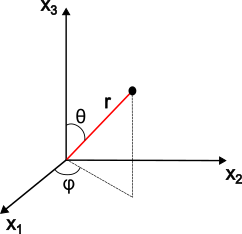
\includegraphics[width=0.24\textwidth]{spheric}  % Adjust width to fit your layout
\end{wrapfigure}

Per scrivere l'operatore momento angolare in coordinate polari basta utilizzare la chain rule, per esempio se consideriamo la prima coordinata cartesiana:
\begin{align*}
	& \frac{\partial}{\partial x_1} = \frac{\partial r}{\partial x_1}\frac{\partial}{\partial r} +\frac{\partial \theta}{\partial x_1}\frac{\partial }{\partial \theta} + \frac{\partial \phi}{\partial  x_1} \frac{\partial}{\partial \phi} = \\[0.4cm]
	& = \sin\theta \cos \phi \frac{\partial}{\partial r} + \cos\theta \cos \phi \frac{1}{r}\frac{\partial}{\partial \theta} - \frac{\sin \phi}{\sin \theta } \frac{1}{r} \frac{\partial}{\partial \phi}
\end{align*}

 analogamente si procede per $\partial \backslash \partial x_2$ e $\partial / \partial x_3$.
\newline

Possiamo quindi scrivere le componenti del momento angolare rispetto alle coordinate polari

\begin{equation}
\begin{aligned}
& \hat{L}_1=i \hbar\left(\cot \theta \cos \phi \frac{\partial}{\partial \phi}+\sin \phi \frac{\partial}{\partial \theta}\right) \\
& \hat{L}_2=i \hbar\left(\cot \theta \sin \phi \frac{\partial}{\partial \phi}-\cos \phi \frac{\partial}{\partial \theta}\right) \\
& \hat{L}_3=-i \hbar \frac{\partial}{\partial \phi}
\end{aligned}
\end{equation}

Osservando l'espressione degli operatori momento angolare notiamo che dipendono solo dagli angoli notevoli e non dalle coordinata radiale r. Dunque lo stato del momento angolare \`e legato alla variazione della direzione degli angoli $\theta$ e $\phi$. La componente $\hat{L}_{3}$ assume una forma particolare rispetto alle altre componenti per via che si \`e scelto $x_3$ come direzione privilegiata nella definizione delle coordinate sferiche.
\newline

\noindent Pe l'operatore momento angolare totale possiamo dare la seguente espressione in coordinate polari data la sua dipendenza dalle singole direzioni 
\begin{equation}
	\bold{\hat{L}}^2 = \hat{L}_{1}^2 + \hat{L}_2^2 + \hat{L}_3^2 = - \frac{\hbar^2}{\sin^2 \theta} \left[ \sin\theta \frac{\partial}{\partial \theta} \left( \sin \theta \frac{\partial}{\partial \theta} \right) + \frac{\partial^2}{\partial \phi^2}\right]
\end{equation} 
Torniamo a considerare la Hamiltoniana associata al problema 
\begin{equation*}
	\hat{H} = - \frac{\hbar^2}{2m} \nabla^2  + V(r) 
\end{equation*}
per portare in coordinate sferiche la Hamiltoniana ci basta trasformare il l'operatore differenziale Laplaciano
\begin{equation}
\nabla^2=\frac{1}{r^2} \frac{\partial}{\partial r}\left(r^2 \frac{\partial}{\partial r}\right)+\frac{1}{r^2 \sin \theta} \frac{\partial}{\partial \theta}\left(\sin \theta \frac{\partial}{\partial \theta}\right)+\frac{1}{r^2 \sin ^2 \theta} \frac{\partial}{\partial \phi^2}
\end{equation}
si osserva che la parte in cui compaiono le derivare rispetto agli angoli coincide con quella dell'operatore di momento angolare totale e dunque possiamo riscriverlo come 
\begin{equation}
\nabla^2=\frac{1}{r^2} \frac{\partial}{\partial r}\left(r^2 \frac{\partial}{\partial r}\right)-\frac{\hat{\mathbf{L}}^2}{\hbar^2 r^2}
\end{equation}
Dato che Hamiltoniana e momento angolare totale commutano tra di loro, abbiamo che gli autostati del momento angolare sono anche autostati della Hamiltoniana. Essendo le autofunzioni associate al momento angolare totale le armoniche sferiche, possiamo pensare ad una soluzione dell'equazione di Schr\"odinger 
\begin{equation}
	\psi(r,\theta,\phi) = R(r)Y_{l,m}(\theta,\phi)
\end{equation}
dove R(r) \`e la funzione d'onda radiale. Tutta la dipendenza angolare \`e data dall'operatore $\hat{\bold{L}}^2$. Sostituendo nell'equazione di Schr\"odinger il termine (3.13) passiamo da un equazione differenziale alle derivate parziali ad un equazione differenziale ordinaria 
\begin{equation*}
	\frac{2mr^2}{R} \left [  - \frac{\hbar^2}{2m} \frac{1}{r} \frac{\partial^2 }{\partial r^2}(rR) + V(r)R -ER\right ] + \frac{\bold{L}^2Y_{l,m}}{Y_{l,m}} = 0
\end{equation*} 
dato che abbiamo due termini dipendenti da coordinate indipendenti distinte l'unica soluzione dell'equazione \`e data da un termine costante, e quindi otteniamo il sistema 
\begin{equation*}
	\left \{ \begin{array}{l}
		\bold{\hat{L}}^2Y_{l,m} = \lambda Y_{l,m} \\[0.4cm]
		\frac{2mr^2}{R} \left [  - \frac{\hbar^2}{2m} \frac{1}{r} \frac{\partial^2 }{\partial r^2}(rR) + V(r)R -ER\right ] = - \lambda
	\end{array}\right.
\end{equation*}
dalla prima equazione sappiamo che il termine $\lambda = \hbar^2l(l+1)$ e di conseguenza la seconda equazione diventa
\begin{equation}
-\frac{\hbar^2}{2 m r^2} \frac{d}{d r}\left(r^2 \frac{d R}{d r}\right)+V_{\text {eff }}(r) R=E R
\end{equation}
dove il termine V(r) \`e stato sostituito dal potenziale efficace 
\begin{equation*}
V_{\mathrm{eff}}(r)=V(r)+\frac{l(l+1) \hbar^2}{2 m r^2}
\end{equation*}
Tale potenziale efficace \`e il medesimo che ritroviamo risolvendo problemi di meccanica classica per un potenziale centrale. Il termine in pi\`u prende il nome di \textit{barriera di momento angolare}. L'unica differenza dalla descrizione classica \`e che il momento angolare \`e quantizzato per unit\`a di $\hbar^2$.

Si osservi che il numero quantistico "m" del momento angolare azimutale non compare nella Hamiltoniana. Dato che $\hat{L}_3$ non dipende dall'autovalore \textit{m}, avremo che lo spettro dell'energia per una qualsiasi particella che si muove in un potenziale centrale sar\`a sempre degenere, con multipli autostati che hanno lo stesso livello di energia. In contrasto l'energia dipende dal numero quantistico del momento angolare totale "l" e dunque ci aspettiamo che ogni autovalore dell'energia ha degenerazione 2l+1, che discende dalle differenti autofunzioni $Y_{l,m}$ con \textit{m} = $-l,-l+1,...,l-1,l$.

Analiticamente possiamo determinare tale risultato scegliendo un ansatz per l'equazione differenziale ordinaria (3.15)
\begin{equation*}
	R(r) = r U(r)
\end{equation*}
sostituendo in (3.15) abbiamo che 
\begin{equation*}
	\frac{-\hbar^2}{2mr} \frac{\partial^2U}{\partial r^2} + \left( rV(r) + \frac{\hbar^2l(l+1)}{2mr} \right)U = EU
\end{equation*}
Verifichiamo che tale ansatz preservi la condizione di normalizzazione di una soluzione dell'equazione di Schr\"odinger 
\begin{equation*}
	1 = \int\bold{ds}|\psi(\bold{s})|^2 = \int_{0}^{+ \infty}dr \; r^2|U(r)|^2 \underbrace{\int d\Omega \; |Y_{l,m}(\theta,\phi)|^2}_{=1}
\end{equation*}
e quindi dobbiamo verificare che 
\begin{equation*}
	\int_{0}^{+ \infty}dr \; r^2|U(r)|^2 =1 
\end{equation*}
e quindi  $U(r) \in L^2([0,+\infty))$ \`e una funzione quadrato integrabile.

\noindent In questo tipo di problemi bisogna prestare attenzione a come si comporta la funzione nell'intorno di r=0 affinch\`e le funzioni siano quadrato integrabili.

Per $r = 0$ il potenziale efficace $V_{eff} \to \infty$. Se un equazione differenziale ha i coefficienti che tendono divergono anche le soluzioni saranno divergenti. Nel nostro caso il termine dato dalla barriera di momento angolare \`e dominante e dunque possiamo scrivere in un intorno di $r=0$ un equazione semplificata trascurando il potenziale
\begin{equation*}
	\frac{-\hbar^2}{2mr}U''(r) + \frac{\hbar^2l(l+1)}{2mr}U(r) \simeq 0
\end{equation*}
otteniamo in questo modo un equazione differenziale di secondo grado
\begin{equation*}
	U'' = l(l+1)U
\end{equation*}
Cerchiamo soluzioni della forma $U(r) = r^\alpha$ che sostituite nell'equazione precedente ci portano all'equazione 
\begin{equation*}
	\alpha(\alpha-1) r^\alpha = l(l+1)r^\alpha 
\end{equation*}
che ammette come soluzioni 
\begin{equation*}
	\alpha_+ = l+1 \quad \text{e} \quad \alpha_- =-l
\end{equation*}
e dunque in un intorno di $r=0$ avremo delle soluzioni della forma
\begin{equation*}
	U_+ (r) = r^{l+1} \quad \text{e} \quad U_{-}(r) = r^{-l}
\end{equation*}
dunque affinch\`e la soluzione del problema rispetti la condizione di normalizzazione considereremo solo 
\begin{equation*}
	U(r) \simeq C_1r^{l+1}
\end{equation*}


\subsection{Interazioni di due punti materiali in un potenziale centrale }
In meccanica classica un sistema a due particelle \`e descritto dalla Lagrangiana
\begin{equation*}
	\mathcal{L}(\bold{r_1},\bold{\dot{r}}_1,\bold{r}_2,\bold{\dot{r}}_2)  = \frac{1}{2}m_1\bold{\dot{r}}^2_1 + \frac{1}{2}m_2\bold{\dot{r}}_2^2 - V(\bold{r}_1 - \bold{r}_2)
\end{equation*}
possiamo semplificare la discussione del problema spostandolo nel sistema di coordinre del centro di massa (o centro di gravit\`a), la posizione del CM \`e descritta dal vettore posizionale 
\begin{equation}
	\bold{r}_{CM} = \frac{m_1\bold{r}_1 + m_2\bold{r}_2}{m_1+m_2}
\end{equation}
mentre le coordinate relativa da 
\begin{equation*}
	\bold{r} = \bold{r}_1 - \bold{r}_2
\end{equation*}
di conseguenza dalla relazione (3.16) possiamo esprimere le posizioni come
\begin{equation*}
	\bold{r}_1 = \bold{r}_{CM} + \frac{m_2}{m_1+m_2}\bold{r} \quad \text{e} \quad \bold{r}_2 = \bold{r}_{CM} - \frac{m_1}{m_1 + m_2}\bold{r}
\end{equation*}
e dunque la Lagrangiana pu\`o essere riscritta rispetto al CM e le posizioni relative 
\begin{align*}
	\mathcal{L}(\bold{r}_{CM},\bold{\dot{r}}_{CM},\bold{r},\bold{\dot{r}}) & = \frac{1}{2}m_1 \left [ \bold{\dot{r}}_{CM} + \frac{m_2}{m_1+m_2}\bold{\dot{r}}\right]^2 + \frac{1}{2}m_2 \left [ \bold{\dot{r}}_{CM} - \frac{m_1}{m_1+m_2}\bold{\dot{r}}\right] - V(\bold{r}) = \\[0.5cm]
	& = \frac{1}{2}M \bold{\dot{r}}_{CM}^2 + \frac{1}{2}\mu \bold{\dot{r}}^2 - V(\bold{r})
\end{align*}
dove 
\begin{equation*}
	M = m_1 + m_2
\end{equation*}
\`e la \textit{massa totale} dele sistema, e:
\begin{equation*}
	\mu = \frac{m_1m_2}{m_1+m_2}
\end{equation*}
\`e la \textit{massa ridotta}. I momenti coniugati rispetto al centro di massa e alla posizione relativa sono dati da
\begin{align*}
	& \bold{p}_{CM} = M \bold{\dot{r}}_{CM} = m_1\bold{\dot{r}}_1 + m_2 \bold{\dot{r}}_2 = \bold{p}_1 + \bold{p}_2 \\[0.5cm] 
	& \bold{p} = \mu \bold{\dot{r}} = \frac{m_2\bold{p_1} - m_1 \bold{p}_{2}}{m_1+m_2}
\end{align*}
dunque possiamo esprimere la Hamiltoniana del sistema in funzione delle nuove variabili dinamiche introdotte
\begin{equation}
	H(\bold{r}_{CM},\bold{p}_{CM},\bold{r},\bold{p}) = \frac{\bold{p}_{CM}^2}{2M} + \frac{\bold{p}^2}{2\mu} + V(\bold{r})
\end{equation}
possiamo passare alla trattazione quantistica considerando le posizioni e i momenti come osservabili del sistema. La Hamiltoniana definita in (3.17) pu\`o essere interpretata come somma di due termini 
\begin{equation*}
	H = H_{CM} + H_{r}
\end{equation*} 
dove 
\begin{equation*}
	H_{CM} = \frac{\bold{p}_{CM}^2}{2M} \quad \text{e} \quad H_r = \frac{\bold{p}^2}{2\mu} + V(\bold{r})
\end{equation*}
dove $[H_{CM},H_{r}] = 0$ commutano tra di loro e dunque esiste una base comune di autovettori di H che sono anche autovettori di $H_{CM}$ e $H_r$; e dunque dobbiamo guardare a delle soluzioni del sistema 
\begin{equation*}
	\left \{ \begin{array}{l}
	H_{CM} |\varphi(\bold{r}_{CM}) \rangle = E_{CM}|\varphi(\bold{r}_{CM}) \rangle  \\
	H_r |\varphi(\bold{r}) \rangle = E_r |\varphi(\bold{r}) \rangle 
	\end{array}\right.
\end{equation*}
dunque possiamo pensare ad una soluzione dell'equazione (3.17) le cui variabili sono separabili 
\begin{equation*}
	|\psi \rangle = | \varphi(\bold{r}_{CM})\rangle |\varphi(\bold{r}) \rangle
\end{equation*}
e quindi l'energia del sistema sar\`a data dal contributo delle singole energie associate alle Hamiltoniane separate 
\begin{equation*}
	E = E_{CM} + E_{r}
\end{equation*}
inoltre la forma esplicita della soluzione \`e data da 
\begin{equation*}
	|\psi \rangle = e^{\frac{i}{\hbar} \bold{p}_{CM} \cdot \bold{r}_{CM}}|\varphi(\bold{r}) \rangle  
\end{equation*}
dove rispetto a $\bold{r}_{CM}$ si ha una componente di moto libero che in meccanica quantistica si traduce in un onda piana.


\section{L'atomo di Idrogeno}

L'atomo di idrogeno \`e il pi\`u semplice degli atomi, essendo costituito da un solo elettrone che orbita attorno al nucleo, mantenendo il suo moto orbitale per via della forza di Coulomb
\begin{equation*}
	F = - \frac{\partial V}{\partial r} = - \frac{e^2}{4\pi \varepsilon_0 r^2}
\end{equation*}
Dove l'elettrone possiede una carica $-e$ e il protone una carica $+e$. La costante $\varepsilon_0$ \`e la permeabilit\`a del mezzo in cui si propaga l'interazione, che di solito consideriamo essere il vuoto. Il potenziale associato alla forza di Coulomb \`e dato da 
\begin{equation*}
	V(r) = - \frac{e^2}{4 \pi \varepsilon_0 r} = - \frac{e^2}{r}
\end{equation*}
che suggerisce una simmetria sferica del problema per la sua invarianza per rotazioni.

Nel nostro caso considereremo solo il moto relativo al \textit{centro di massa}. La Hamiltoniana che descrive il moto relativo delle due  particelle \`e dato da
\begin{equation*}
	H(\bold{r},\bold{p}) = \frac{\bold{p}^2}{2\mu} - \frac{e^2}{r}
\end{equation*} 
Dato che $m_p \gg m_e$, la massa ridotta $\mu$ del sistema \`e approssimabile a $m_e$:
\begin{equation*}
	\mu = \frac{m_em_p}{m_e+m_p} \simeq m_e \left( 1 - \frac{m_e}{m_p}\right)
\end{equation*}
Questo vuol dire che il centro di massa del sistema coincide con la posizione del protone, e con buona approssimazione possiamo identificare la particella relativa con l'elettrone.

\subsection{Il modello di Bohr }

Diamo un introduzione classica al modello orbitale introdotto da Bohr per l'atomo d'idrogeno anche se questo \`e incompatibile con la trattazione quantistica. Questo modello semi-classico \`e basato sull'idea che un elettrone compia un orbita circolare di raggio r attorno al protone, obbedendo alle seguenti equazioni 
\begin{equation*}
	E = \frac{1}{2}\mu v^2 - \frac{e^2}{r} \quad \text{e} \quad \frac{\mu v^2}{r} = \frac{e^2}{r}
\end{equation*}
che esprimono rispettivamente l'energia totale del sistema, e la seconda non \`e altro che l'equazione fondamentale della dinamica di Newton. La seguente espressione 
\begin{equation*}
	\mu vr = n \hbar \quad n \in \mathbb{N}
\end{equation*}
introduce la condizione di quantizzazione introdotta empiricamente da Bohr per spiegare i livelli discreti dell'energia, postulando che le uniche orbite ammesse sono quelle che soddisfano tale equazione.
Mediante semplici passaggi algebrici possiamo definire le grandezza $E_n, r_n$ e $v_n$:
\begin{equation*}
	E_n = - \frac{1}{n^2}E_I \quad r_n = n^2a_0 \quad v_n = \frac{1}{n}v_0
\end{equation*}
dove 
\begin{equation*}
	E_I = \frac{\mu e^4}{2h^2} \quad a_0 = \frac{\hbar^2}{\mu e^2} \quad v_0 = \frac{e^2}{\hbar}
\end{equation*}
dove rispettivamente abbiamo che $E_I $ rappresenta \textit{l'energia di ionizzazione} dell'atomo d'idrogeno (sarebbe l'energia che dobbiamo fornire all'atomo nel suo stato fondamentale per rimuovere l'elettrone), mentre $a_0$ prende il nome di \textit{raggio di Bohr} e caratterizza la dimensione atomica. Sperimentale si ha che 
\begin{equation*}
	E_I \simeq 13.6 \; eV \quad \text{e} \quad a_0 \simeq 0.52 \; \mathring{A} 
\end{equation*}

\subsection{Descrizione Quantistica dell'atomo d'idrogeno}

La descrizione quantistica dell'atomo d'idrogeno si riconduce a quanto discusso per due punti materiali in un potenziale centrale, di conseguenza possiamo definire la Hamiltoniana del moto relativo come 
\begin{equation*}
	\hat{H} = \frac{\bold{\hat{p}}_{r}^2}{2 \mu} + \underbrace{\frac{\bold{\hat{L}}^2}{2mr^2} - \frac{e^2}{r}}_{= V_{eff}}
\end{equation*}
Riprendendo la trattazione della sezione precedente avremo che la soluzione sar\`a caratterizzata da tre numeri interi \textit{n}, \textit{l} e \textit{m} tali che:
\begin{itemize}
	\item \textit{n} identifica gli stati di energia discreti per $n \in \mathbb{N}$, che nel contesto dell'atomo di idrogeno viene definito \textit{numero quantistico principale}.
	\item \textit{l} indica il momento angolare quantizzato e compare nell'autovalore di $\bold{\hat{L}}^2$ come $l(l+1)\hbar^2$.
	\item \textit{m} \`e il momento angolare azimutale, che compare per convenzione come autovalore $m\hbar$ di $\hat{L}_3$.
\end{itemize}
Cerchiamo come soluzione dell'equazione di Schr\"odinger una funzione della forma 
\begin{equation*}
	\psi(r, \theta, \phi) = R(r)Y_{lm}(\theta,\phi) = \frac{1}{r}U(r)Y_{lm}(\theta,\phi)
\end{equation*}
e l'equazione di Schr\"odinger dell'atomo di idrogeno \`e data da 
\begin{equation}
	-\frac{\hbar^2}{2m_e}U''(r) + \left ( -\frac{e^2}{r} + \frac{\hbar^2l(l+1)}{2m_er^2}\right)U(r) = EU(r)
\end{equation}

\subsubsection{Spettro dell'energia }
La Hamiltoniana H possiede sia uno spettro discreto (per valori negati degli autovalori) che un spettro continuo (per valori positivi degli autovalori). Per $E > 0 $ come in figura abbiamo che il moto classico non \`e limitato verso destra, ma \`e limitato in prossimit\`a del punto A.

\begin{wrapfigure}{r}{0.5\textwidth} % 'r' for right, width of the figure
    \centering
    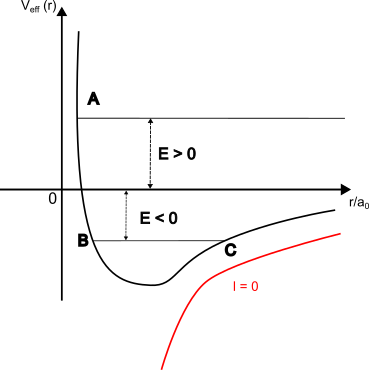
\includegraphics[width=0.48\textwidth]{potenzialEff}
    \caption{Potenziale efficace per $l \neq 0$ e $l = 0$}
\end{wrapfigure}

Come risultato l'equazione (3.18) possiede una soluzione accettabile per ogni $E > 0 $ e quindi H possiede uno spettro continuo le cui autofunzioni associate non sono quadrato integrabili. Dall'altro lato per $E < 0 $ il moto classico \`e limitato, dato che viene confiato tra i punti B e C in figura e dunque l'equazione (3.18) ammette solo soluzioni per valori discreti dell'energia E. Le autofunzioni associate allo spettro discreto di H sono funzioni quadrato integrabili.


Iniziamo la determinazione esplicita delle soluzioni partendo dagli stati legati dai da $E < 0$. Riscriviamo l'equaziona (3.18) effettuando delle opportune sostituzioni definendo le grandezze 

\begin{equation*}
	\rho = \frac{r}{a_0} \quad \text{e} \quad \lambda = \sqrt{-\frac{E}{E_I}}
\end{equation*}
in questo modo l'equazione di Schr\"odinger assume la forma 

\begin{equation}
	\left ( \frac{d^2}{d\rho^2} - \frac{l(l+1)}{\rho^2}+\frac{2}{\rho} - \lambda^2 \right )U(\rho) = 0 
\end{equation}

Per $r \to \infty$ possiamo approssimare (3.19) all'equazione differenziale di un oscillatore armonico
\begin{equation*}
	U''-\lambda^2U = 0
\end{equation*} 
che ha come soluzione 
\begin{equation*}
	U_{\pm}(\rho) = e ^{\pm \lambda \rho}
\end{equation*}
che per $\rho \to \infty$ la funzioen diverge o tende a 0. Per studiare gli stati legati consideriamo la soluzione negativa $U(\rho) = e^{-\lambda\rho}$ dato che la funzione deve essere quadrato integrabile. Per $\rho$ molto piccoli ritroviamo quanto discusso per i due corpi in campo centrale ritrovando l'equazione
\begin{equation*}
	\rho^2U''(\rho) - l(l+1)U = 0 
\end{equation*}
che ha per soluzione $U_{-}(\rho) = \rho^{-l}$ e $U_{+}(\rho) = \rho^{l+1}$ e siccome abbiamo bisogno di funzioni quadrato integrabili anche in questo caso teniamo
\begin{equation*}
	U_{+}(\rho) = \rho^{l+1}
\end{equation*}
Effettuiamo un cambio di variabili andando a considerare $U(\rho) = e^{-\lambda \rho}y(\rho)$ e quindi
\begin{align*}
	U'(\rho) = & \;y'e^{-\lambda \rho} - \lambda y e^{-\lambda \rho} \\[0.3cm]
	U''(\rho) = & \; y''e^{-\lambda \rho} - 2 \lambda y'e^{-\lambda \rho} + \lambda^2e^{-\lambda \rho}
\end{align*}

sostituendo nell'equazione (3.19) otteniamo 
\begin{equation}
	\left [ \frac{d^2}{d\rho^2} - 2 \lambda \frac{d}{d\rho} + \left( \frac{2}{\rho} - \frac{l(l+1)}{\rho^2}\right) \right ]y = 0
\end{equation}
in questo modo si ha un equazione differenziale del secondo ordine rispetto alla variabile $\rho$. Usiamo come ansatz la soluzione in seri di potenze 
\begin{equation*}
	y(\rho) = \rho^s \sum_{k=0}^{\infty}c_k \rho^{k} = \sum_{k=0}^{\infty} c_k \rho^{k+s}
\end{equation*}
sostituendo in (3.20) si ha l'equazione differenziale
\begin{equation}
	\sum_{k=0}^{\infty}c_k \left [ (k+s)(k+s-1)\rho^{k+s-2} -2\lambda (k+s)\rho^{k+s-1} + 2\rho^{k+s-1} -  l(l+1)\rho^{k+s -2}\right ] = 0 
\end{equation}
affinch\`e la serie sia nulla tutti i coefficienti devono essere uguali a 0. Il coefficiente di ordine minore \`e dato da $\rho^{s-2}$ per $k=0$ e dunque otteniamo l'equazione del primo termine
\begin{equation*}
	[-l(l+1) + s(s-1)]c_0 = 0 
\end{equation*}
dato che per definizione $c_0 \neq 0$ si ha che \textit{s} pu\`o assumere solo due valori
\begin{equation*}
	\left \{ \begin{array}{l}
		s_1 = l+1 \\
		s_2 = -l
	\end{array}\right.
\end{equation*}
affinch\`e la soluzione sia quadrato integrabile escludiamo la soluzione $s_2$, dunque sostituendo $s_1 = l+1$ in (3.21) abbiamo che
\begin{equation*}
		\sum_{k=0}^{\infty}c_k \left [ (k+l+1)(k+l)\rho^{k+l-1} -2\lambda (k+l+1)\rho^{k+l} + 2\rho^{k+l} -  l(l+1)\rho^{k+l -1}\right ] = 0 
\end{equation*}
se consideriamo i termini successivi $k+1$ sulle sommatorie in cui compare $\rho^{k+l-1}$ abbiamo che
\begin{equation*}
	\sum_{k=0}^{\infty}\rho^{k+l} \left \{  c_{k+1}(k+l+2)(k+l+1) -2\lambda c_k \left [(k+l+1)+2 \right]-c_{k+1}l(l+1)\right \} = 0
\end{equation*}
di conseguenza ogni termine 
\begin{align*}
	 & c_{k+1}(k+l+2)(k+l+1) -2\lambda c_{k} \left [(k+l+1)+2 \right]-c_{k+1}l(l+1) = 0 \\[0.4cm]
	 & \iff c_{k+1}[(k+1)(k+2l+2)] - 2c_{k}[\lambda(k+l+1)-1] = 0 \\[0.4cm]
	 & \Rightarrow c_{k+1} = \frac{\lambda(k+l+1)-1}{(k+1)(k+2l+2)}2c_{k} 
\end{align*}
dove il termine iniziale $c_0$ \`e fissato dalle condizioni iniziali ed \`e arbitrario. Di conseguenza la serie di potenze soluzione dell'equazione differenziale \`e data da 
\begin{equation}
	y(\rho) = \sum_{k=0}^{\infty} c_k \rho^{k+l+1}
\end{equation}
Affinch\`e la componente radiale  della soluzione dell'equazione di Schr\"odinger $U(\rho) = y(\rho)e^{-\lambda \rho}$ sia una funzione quadrato integrabile abbiamo bisogno di capire se $y(\rho)$ \`e limitata per $\rho \to \infty$ o al pi\`u ha un ordine d'infinito minore di quello dell'esponenziale. Per studiare l'andamento della serie di potenze al crescere di k osserviamo che 
\begin{equation*}
	k \to \infty \quad \frac{c_{k+1}}{c_k} \sim \frac{2\lambda k}{k^2} \sim \frac{2\lambda }{k} \to 0 
\end{equation*}
e dunque la serie \`e convergente $\forall \rho \in \mathbb{R}$. Essendo i coefficiente della serie definiti ricorsivamente dal rapporto precedente possiamo dedurre che 
\begin{equation*}
	c_k = \frac{(2\lambda)^k}{k!}
\end{equation*}
e  
\begin{equation*}
	y(\rho) = \rho^{l+1}\sum_{k=0}^{\infty} \frac{(2\lambda)^k}{k!}\rho^k \sim \rho^{l+1}e^{2\lambda \rho}
\end{equation*}
dunque la soluzione dell'equazione di Schr\"odinger assume la forma 
\begin{equation*}
	U(\rho)= \rho^{l+1}e^{\lambda \rho} \not\in L^2
\end{equation*}
per un qualsiasi generico valore $\lambda$.  Per poter trovare una soluzione accettabile abbiamo bisogno di quantizzare il termine $\lambda $ e quindi rigettare tutti i casi in cui l'espansione (3.22) possiede un numero infinito di termini. Di conseguenza abbiamo bisogno d'imporre che per un certo valore $\overline{k}$ il corrispondente coefficiente $c_{k} = 0$ e quindi per via della reiterativit\`a che lega i coefficienti tra loro avremo che i termini successivi $c_{k+1}=0$, in questo modo abbiamo che la serie infinita viene troncata ad una serie finita, diventando un polinomio $P_k(\rho)$. 
Fissato il temine k, l'imposizione di avere $c_k = 0$ ci porta ad avere la quantizzazione di $\lambda$
\begin{equation*}
	\lambda  = \frac{1}{l+1}
\end{equation*} 
dato che il termine $\lambda$ \`e legato all'energia avremo un espressione della sua quantizzazione
\begin{equation}
	E_{k,l} = -\frac{E_I}{(k+l)^2} \quad k \in \mathbb{Z}^+
\end{equation}
In conclusione $y(\rho)$ corrisponde ad un polinomio il cui termine di ordine minimo \`e dato da $\rho^{l+1}$ e il termine massimo \`e $\rho^{k+l}$. In particolare il polinomio associato prende il nome di \textit{polinomio di Laguerre} e dunque la soluzione dell'equazione (3.18) \`e data 
\begin{equation*}
	U_{k,l}(\rho) = C \rho^{l+1}L^{2l+1}_{k}(2\rho) e^{-\frac{\rho}{l+1}} 
\end{equation*}
dove il polinomio di Laguerre generalizzato \`e definito come
\begin{equation*}
	L_{n}^{m}(x) = \frac{1}{n!} \frac{e^x}{x^m} \frac{d^n}{dx^n}e^{-x}x^{n-m}
\end{equation*}

\subsubsection{Livelli di energia}
Per ogni valore fissato di $l$, esiste un numero infinito di possibili valore dell'energia per $k \in \mathbb{Z}^+$; ciascuno di essi ha almeno una degenerazione di $2l+1$ termini, tale degenerazione \`e data dal fatto che le equazioni radiali dipendono solo dal numero quantico $l$ e non da $m$. L'equazione (3.23) ci dice che due autovalori $E_{k,l}$ e $E_{k',l'}$ corrispondenti a differenti equazioni radiali ( $l \neq l'$) sono uguali se solo se $k+l = k' + l'$. Nel caso dell'atomo di idrogeno, $E_{k,l}$ non dipende da $k$ e $l$ separatamente, ma dalla loro somma.
\begin{equation*}
	n = k+l
\end{equation*}

\noindent Quindi i diversi livelli di energia possono essere espressi rispetto al numero quantico $n \geq 1$ e possiamo riscrivere (3.23) nel seguente modo
\begin{equation}
	E_n = -\frac{1}{n^2}E_I
\end{equation}
Sappiamo che $n$ \`e definito come \textit{numero quantico principale} e per un suo determinato valore si ha quella che viene definita \textit{shell elettronica}. Dato che $k$ \`e un numero intero maggiore e uguale di 1, il termine $l$ possiede un numero finito di valori che pu\`o assumere per $n$ fissato.
\begin{equation*}
	l = 0,1,2,...,n-1
\end{equation*}
Tale risultato ci dice che per ciascuna shell caratterizzata da $n$ si hanno n sub-shells, ciascuna corrispondente ad un valore che pu\`o assumere $l$. Ad ogni sub-shell sono associati $(2l+1)$ stati distinti, dati dai valori possibili valori di $m$ per $l$ fissato. La generazione totale per un livello di energia $E_n$ \`e data da
\begin{equation*}
	g_n = \sum_{l=0}^{n-1}(2l+1) = 2\frac{(n-1)n}{2} + n = n^2
\end{equation*}

\begin{figure}[!ht]
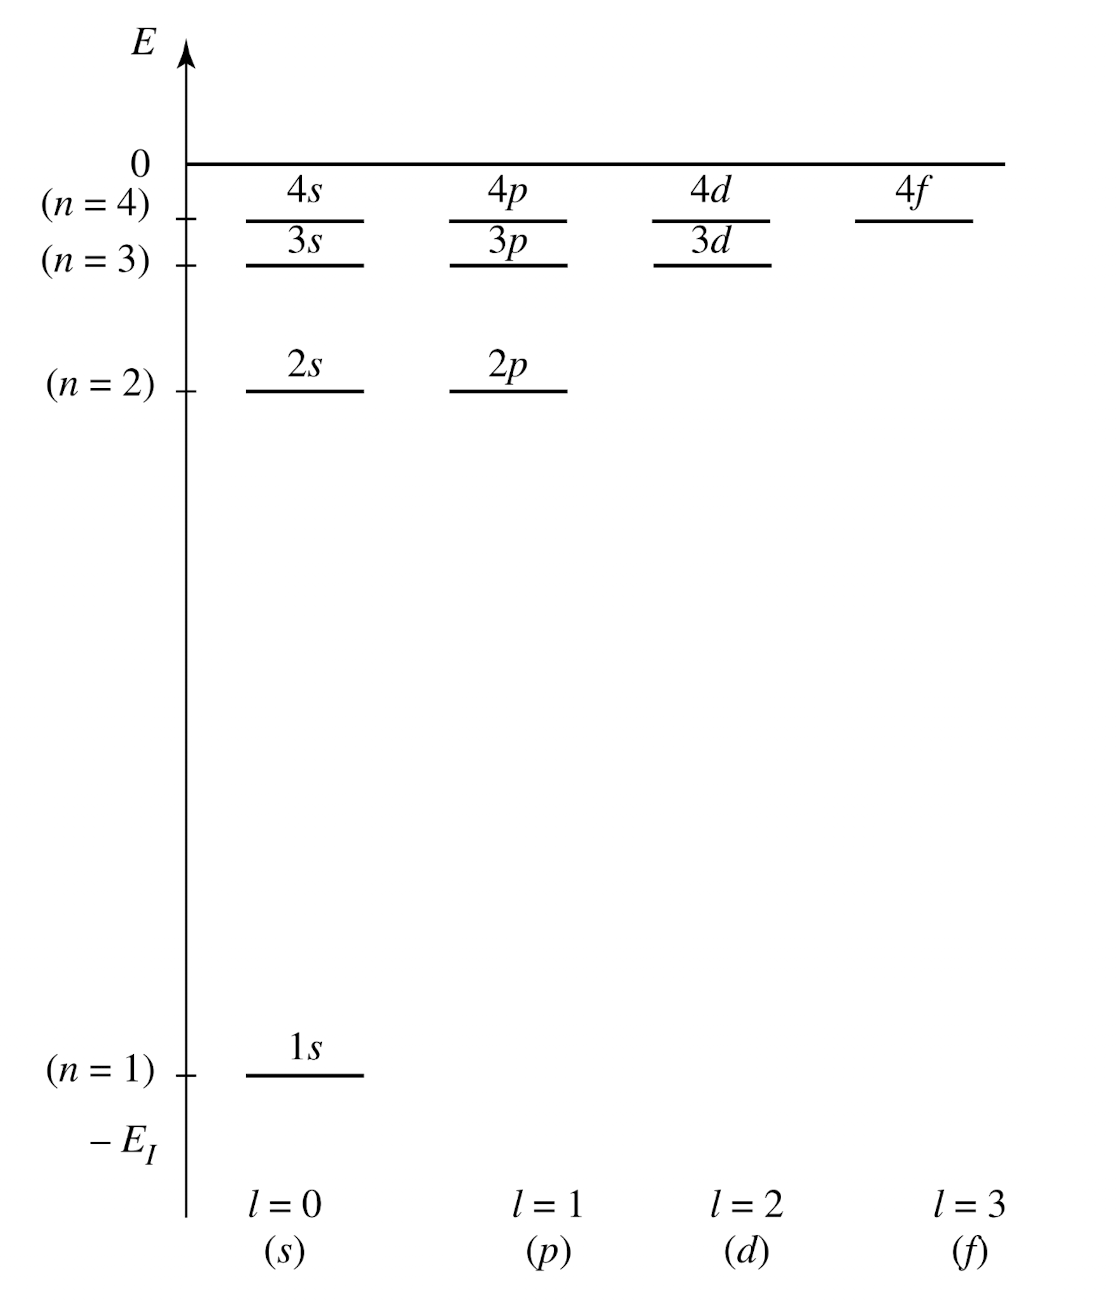
\includegraphics[width = 10cm]{energydeg}	
\centering
\end{figure}

\newpage

Lo stato fondamentale per $n=1$ \`e unico ed \`e dato per $l =0 $, inoltre in fisica atomica al variare di $l$, le armoniche sferiche definiscono diverse nomenclature di onde, in questo caso la categoria associata \`e quella delle \textit{s-wave}. Per $n=2$ ci sono quattro stati eccitati complessivamente che corrispondo a uno nelle \textit{s-wave} e tre per $l=1$ nelle \textit{p-wave}. Nel caso $n=3$ avremo nove stati eccitati complessivi, corrispondenti rispettivamente a uno nelle \textit{s-wave}, tre nelle \textit{p-wave} per $l=1$ e cinque per $l=2$ nelle \textit{d-wave}. E cos\`i via.
\newline

Lo spettro di energia descritto dalla quantizzazione dell'energia (3.24) non descrive completamente l'atomo di idrogeno. Ci sono delle correzioni da fare dovute alla relativit\`a speciale.Queste correzioni dividono le $n^2$ degenerazioni in modo tale che lo stesso stato per differenti $l$ ha diverse energie. Questa suddivisione \`e dell'ordine di $\alpha^4$, che sono maggiori di quelle originali di ordine $\alpha^2$, e sono definite come la \textit{struttura fine} dell'atomo di idrogeno. Parleremo di questo risultato nei prossimi capitoli.

\subsubsection{La funzione d'onda }

 La funzione d'onda soluzione dell'equazione di Schr\"odinger \`e data da 
 \begin{equation*}
 	\psi_{n,l,m}(r,\theta,\phi) = \frac{1}{r}U_{n,l}(r)Y_{l,m}(\theta,\phi) 
 \end{equation*}
dove si \`e espressa la componente radiale della soluzione rispetto a numero quantico $n$ anzich\`e $k$. Il termine $Y_{l,m}$ costituisce la parte angolare della soluzione data dalle funzioni armoniche sferiche.
Di seguito si ripotano le espressioni analitiche di alcune armoniche sferiche


\begin{equation*}
	\begin{array}{l}
		Y_{0,0} = \frac{1}{\sqrt{4 \pi}} \\[0.5cm]
		Y_{1,0} = \sqrt{\frac{3}{4 \pi}}\cos\theta \simeq \frac{z}{r}\\[0.5cm]
		Y_{1,1} = - \sqrt{\frac{3}{8\pi}}\sin \theta e^{i\phi} \simeq \frac{x+iy}{r}\\[0.5cm]
		Y_{1,-1} = \sqrt{\frac{3}{8\pi}}\sin \theta e^{-i\phi} \simeq \frac{x-iy}{r}\\[0.5cm]
		Y_{2,0} = \sqrt{\frac{5}{16 \pi}}(3\cos^2\theta -1) \simeq \frac{2z^2-x^2-y^2}{r^2} \\[0.5cm]
		Y_{2,1} = - \sqrt{\frac{15}{8\pi}}\sin\theta \cos\theta e^{i\phi} \simeq \frac{(x+iy)z}{r^2} \\[0.5cm]
		Y_{2,-1} =  \sqrt{\frac{15}{8\pi}}\sin\theta \cos\theta e^{-i\phi} \simeq \frac{(x-iy)z}{r^2}\\[0.5cm]
		Y_{2,2} = \sqrt{\frac{15}{32 \pi}}\sin^2\theta e^{2i\phi} \simeq \frac{(x+iy)^2}{r^2}\\[0.5cm]
		Y_{2,-2} = \sqrt{\frac{15}{32 \pi}}\sin^2\theta e^{-2i\phi} \simeq \frac{(x-iy)^2}{r^2}\\[0.5cm] 
	\end{array}
\end{equation*}

\newpage 

Per le armoniche sferiche la densit\`a di probabilit\`a associata dipender\`a solo dalla variabile angolare $\theta$ e dunque \`e invariante per rotazione attorno all'asse $x_3 = z $.
\begin{equation*}
	|Y_{l,m}(\theta,\phi)|^2 = P(\theta) 
\end{equation*}
di seguito riportiamo alcuni grafici della densit\`a di probabilit\`a per le armoniche sferiche definite in precedenza 
 
\begin{figure}[!ht]
\vspace{0.1in}
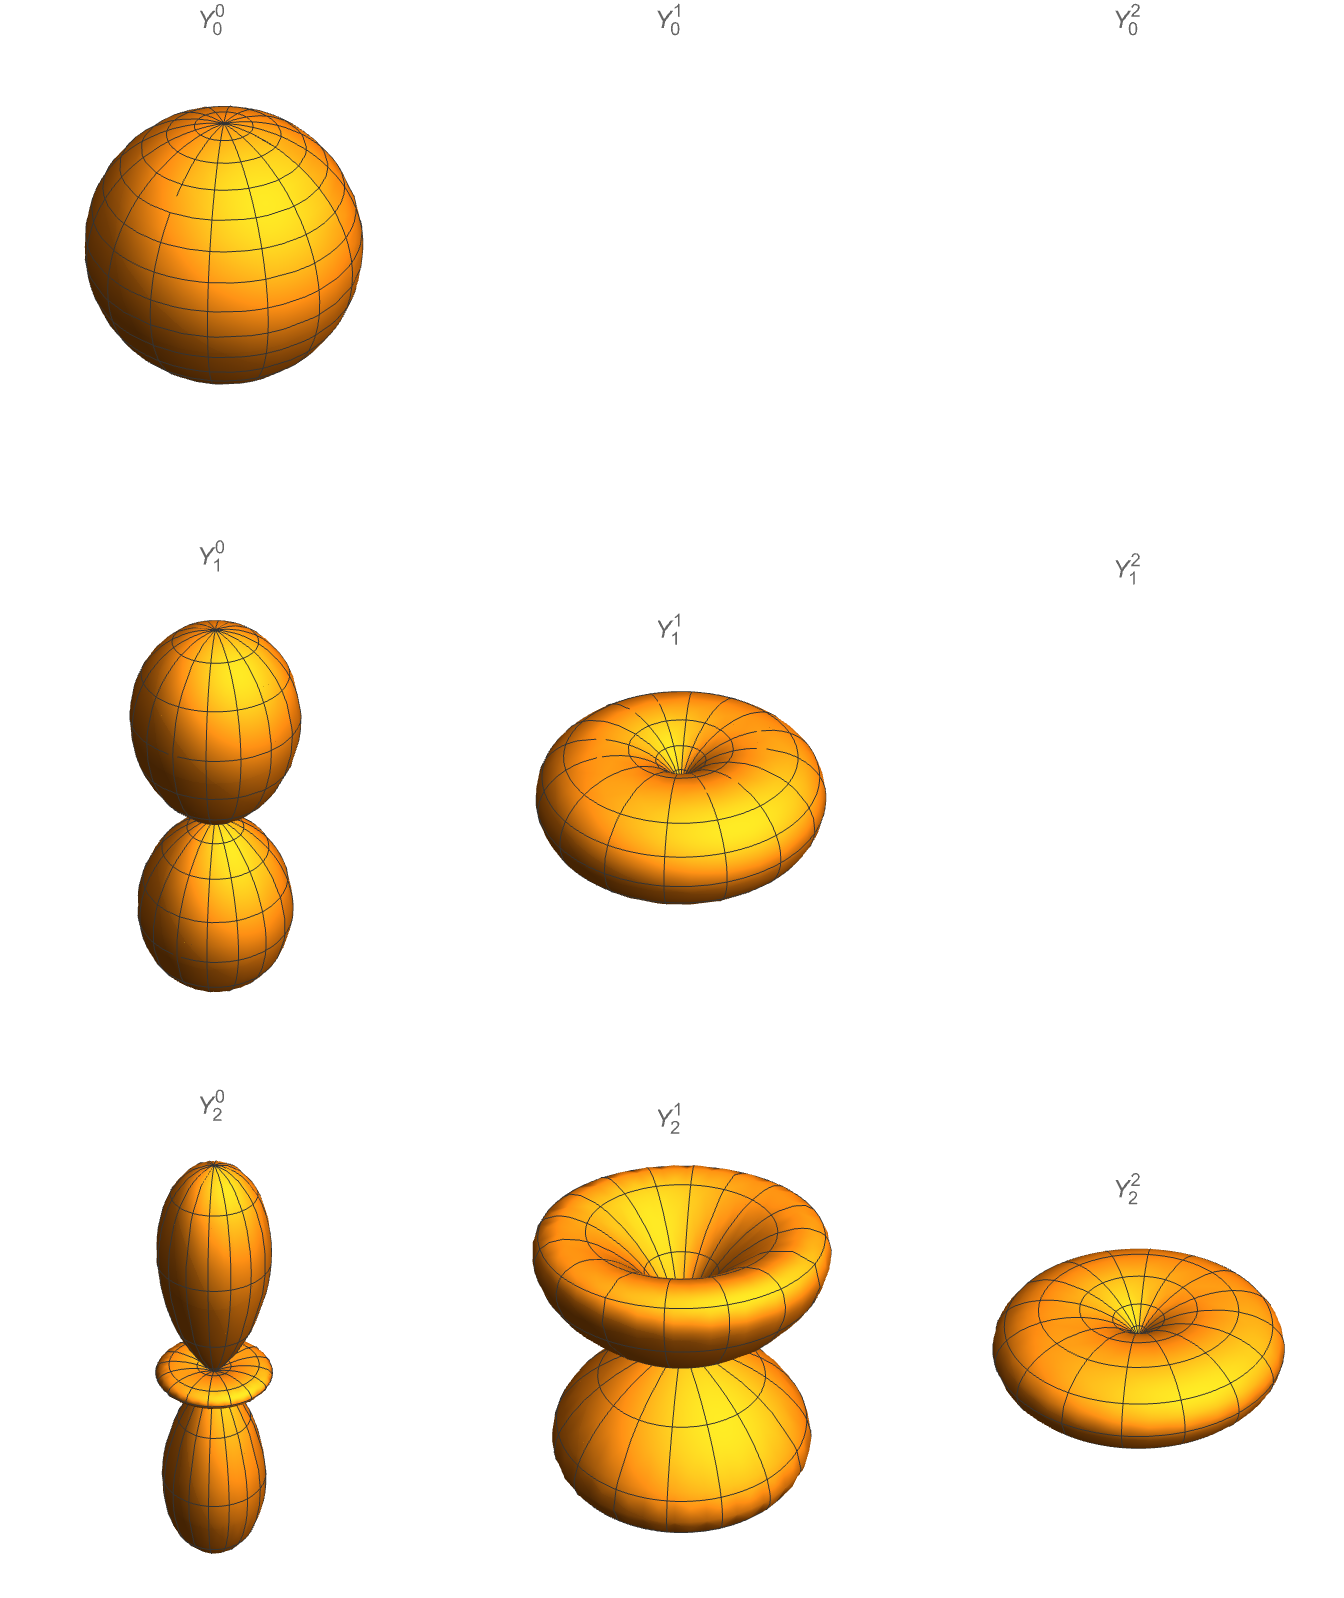
\includegraphics[width = 10cm]{harmonicDensity}	
\centering
\vspace{0.1in}
\caption{Densit\`a di probabilit\`a per un armonica sferica al variare di l=0,1,2}
\end{figure}
\begin{lstlisting}[language=Python, caption= Mathematica Snippet, numbers=left, frame=single]
# Probability Density plot for spherical harmonic function

Y[l_, m_] := SphericalHarmonicY[l, m, \[Theta], \[Phi]]
Ybar[l_, m_] := SphericalHarmonicY[l, -m, \[Theta], \[Phi]] 

 P[l_, m_] := Y[l, m]*Ybar[l, m]
 
SphericalPlot3D[
 Evaluate[P[l, m], {\[Theta], 0, Pi}], {\[Phi], 0, 2 Pi}, 
 Boxed -> False, Axes -> None]
\end{lstlisting}

\section{Oscillatore Armonico in 1D}

L'oscillatore armonico \`e il nome che si da ad un sistema in cui si muove una particella sotto l'azione di un potenziale quadratico. In meccanica classica, l'energia \`e data da 
\begin{equation*}
	E = \frac{1}{2}m \dot{x}^2 + \frac{1}{2}m\omega^2x^2
\end{equation*}
L'equazione classica del moto discende dal fatto che l'energia \`e conservata, che significa $\dot{E} = 0$ che equivale a 
\begin{equation*}
	\ddot{x} = - \omega^2x
\end{equation*}
La soluzione generale dell'equazione \`e data da $x(t) = A\cos(\omega(t-t_0))$ e descrive il moto di una particella che si muove avanti e indietro con frequenza $\omega$. Sostituendo nell'equazione dell'energia del sistema si ha che 
\begin{equation*}
	E = \frac{m\omega^2}{2}A^2
\end{equation*}

e quindi essendo $E \geq 0$ ci si ritrova in una condizione classica. L'energia non \`e quantizzata viene fissata dal valore dell'ampiezza dell'oscillazione.

\subsection{Teoria pre-quantistica Bohr-Sommerfeld}

La quantizzazione di Bohr-Sommerfeld \'e un'estensione del modello atomico di Bohr sviluppata da Arnold Sommerfeld per spiegare fenomeni che il modello originale di Bohr non riusciva a descrivere, come l’effetto Zeeman e lo sdoppiamento delle linee spettrali. Sommerfeld, ampliando l’idea di quantizzazione introdotta da Bohr, propose che non solo il momento angolare dell’elettrone fosse quantizzato, ma anche altre caratteristiche dell’orbita, come la forma e l’orientamento.
\newline

\noindent Questa teoria si basa su due postulati principali:
\begin{enumerate}
	\item \textbf{Orbitalit\`a ellittica:} Sommerfeld introdusse orbite ellittiche per gli elettroni, parametrizzandole con un numero quantico principale  n  (come in Bohr) e un numero quantico azimutale  k  (legato alla forma dell’ellisse). Questo port\`o alla definizione di livelli energetici con diversa forma e dimensione, spiegando la struttura fine degli spettri atomici.

	\item \textbf{Quantizzazione dell'azione:} L'azione (intesa come integrale lungo un'orbita chiusa del momento in funzione della coordinata generalizzata) deve essere un multiplo intero della costante di Planck ridotta ( $h/2\pi$ ). In termini matematici, questo si esprime come:
	\begin{equation*}
		\frac{1}{2\pi}\oint dq \; p = n \hbar
	\end{equation*}
	dove  $p$  è il momento coniugato alla coordinata  $q$ , e  $n$  è un numero intero chiamato "numero quantico". Questo implica che le orbite possibili non sono continue, ma discrete.
\end{enumerate}
Il secondo postulato induce anche la quantizzazione dell'energia, infatti considerando il periodo di percorrenza di un orbita chiusa, che \`e pari a $T = \frac{2 \pi}{\omega}$, possiamo riscrivere l'azione nel seguente modo
\begin{align*}
	\frac{1}{2\pi} \oint dx\; m\dot{x} & =  \frac{1}{2\pi} \oint m \dot{x} \frac{dx}{dt}dt = \frac{1}{2\pi} \int_{0}^{T} dt\; m\dot{x}^2 = \\[0.5cm]
	& = \frac{1}{2\pi} mA^2\omega^2 \int_{0}^{T}dt \;  \sin^2(\omega t + \phi) = \\[0.5cm]
	& =  \frac{1}{2\pi}mA^2\omega^2 \frac{\pi}{\omega} = \frac{1}{2}m\omega A^2 = n\hbar \\[0.5cm]
	& \Rightarrow E_n = \frac{1}{2}m\omega^2A^2 = n \hbar \omega \quad n \in \mathbb{Z}^+
\end{align*}

\noindent Il modello di Bohr-Sommerfeld \`e stato un importante passo avanti verso una descrizione pi\`u accurata dei livelli energetici degli atomi, ma successivamente \`e stato superato dalla meccanica quantistica moderna, che con la teoria ondulatoria di Schr\"odinger e il principio di indeterminazione di Heisenberg ha permesso una comprensione pi\`u completa e precisa dei fenomeni atomici.
 
 \subsection{Trattazione quantistica dell'oscillatore armonico}
 Definiamo l'equazione di Schr\"odinger associata al sistema dell'oscillatore armonico come 
 \begin{equation}
 	-\frac{\hbar^2}{2m}\frac{d^2\psi}{dx^2} + \frac{1}{2}m \omega^2x^2\psi = E \psi
 \end{equation}
Prima di procedere a determinare le soluzioni dell'equazione, osserviamo alcune importanti propriet\`a deducibili dalla funzione dell'energia potenziale
\begin{enumerate}
	\item \textit{Gli autovalori della Hamiltoniana sono positivi}. Si dimostra che se un potenziale $V(x)$ \`e limitato inferiormente gli autovalori di un Hamiltoniana della forma $H = \frac{P^2}{2m} + V(x)$ devono essere maggiori del minimo del potenziale. Per l'oscillatore armonico, abbiamo che il potenziale ha minimo $V_m = 0$.
	\item \textit{Le autofunzioni di H hanno una parit\`a definita}. Tale risultato \`e dovuto al fatto che il potenziale V(x) \`e una funzione pari $V(x) = V(-x)$.
	\item \textit{Lo spettro dell'energia \`e discreto}. Per qualsiasi valore dell'energia, classicamente il moto \`e limitato ad una regione definita del piano, e si dimostra che di conseguenza gli autovalori della Hamiltoniana formano un insieme discreto. 
\end{enumerate}

\subsubsection{ Gli operatori $\hat{X}$ e $\hat{P}$}

Gli osservabili X e P hanno dimensione rappresentando rispettivamente posizione e momenti definiamo gli operatori
\begin{equation*}
	\hat{X} = \sqrt{\frac{m\omega}{\hbar}}X \quad \text{e} \quad \hat{P} = \frac{1}{\sqrt{m\hbar\omega}}P
\end{equation*}
che sono adimensionali.

Utilizzando questi nuovi operatori, la relazione di commutazione canonica assume la forma 
\begin{equation*}
	[\hat{X},\hat{P}] = i
\end{equation*}
e la Hamiltoniana dee; sistema assume la forma 
\begin{equation*}
	H = \hbar \omega \hat{H}
\end{equation*}
dove 
\begin{equation}
	\hat{H} = \frac{1}{2}(\hat{X}^2 + \hat{P}^2)
\end{equation}
utilizzando un Hamiltoniana definita in questo modo andremo a determinare sia autofunzioni, che autovalori adimensionali.

\subsubsection{Gli operatori $a$, $a^\dag$ e $N$}

Definiamo gli operatori 
\begin{equation}
	a = \frac{1}{\sqrt{2}}(\hat{X} + i \hat{P}) \quad \text{e} \quad a^{\dag} = \frac{1}{\sqrt{2}}(\hat{X} - i \hat{P})
\end{equation}
che possiamo invertire definendo una nuova forma degli operatori posizione e momento 
\begin{equation*}
	\hat{X} = \frac{1}{\sqrt{2}}(a^\dag + a) \quad \text{e} \quad \hat{P} = \frac{i}{\sqrt{2}}(a^\dag-a) 
\end{equation*}
Gli operatori $a$ e $a^\dag$ non sono Hermitiani , ma sono rispettivamente autoaggiunti. Il commutatore di $a$ e $a^\dag$ \`e dato da
\begin{equation*}
	[a,a^\dag] = \frac{1}{2}\left [\hat{X}+i\hat{P},\hat{X}-i\hat{P}\right ] = \frac{i}{2}\left [ \hat{P},\hat{X}\right]-\frac{i}{2} \left[\hat{X},\hat{P} \right] = 1
\end{equation*}
In ultimo introduciamo l'operatore $N$ dato da
\begin{equation*}
	N = a^\dag a = \frac{1}{2}(\hat{X} - i \hat{P})(\hat{X}+i\hat{P}) = \frac{1}{2}(\hat{X}^2+\hat{P}^2 + i\hat{X}\hat{P} - i \hat{P}\hat{X}) = \frac{1}{2}(\hat{X}^2 + \hat{P}^2-1)
\end{equation*}
tale operatore ci permette di riscrivere la Hamiltoniana in (3.26) nel seguente modo
\begin{equation}
	\hat{H} = N - \frac{1}{2}
\end{equation}
La non commutativit\`a di $\hat{X}$ e $\hat{P}$ sono all'origine del termine aggiuntivo $1/2$ che compare nell'equazione precedente.

L'operatore $N$ \`e Hermitiano dato che 
\begin{equation*}
	N^\dag = a^\dag(a^\dag)^{\dag} = a^\dag a = N 
\end{equation*}
Dall'equazione (3.28) abbiamo che gli autovettori di $\hat{H}$ sono autovettori di $N$ e viceversa. Infine calcoliamo la commutazione di N con gli operatori $a$ e $a^\dag$:
\begin{align*}
	[N,a] = [a^\dag a, a] = a^{\dag}[a,a]+a[a^\dag,a] = - a \\[0.4cm] 
	[N,a^\dag] = [a^\dag,a] = a^\dag[a,a^\dag]+ [a^\dag,a^\dag]a = a^\dag
\end{align*}
Gli operatori definiti ci permettono di derivare lo spettro e le autofunzioni dell'oscillatore armonico senza risolvere direttamente l'equazione di Schr\"odinger. 



Lo determinazione degli autovalori di H, diventa lo studio degli autovalori dell'operatore N per la definizione (3.28) che lega le due grandezze.
\begin{equation*}
	N|\nu \rangle = \nu |\nu \rangle
\end{equation*}
dove $|\nu \rangle = | \psi_{\nu} \rangle $ funzione d'onda. Quando questa equazione viene risolva avremo che gli autovalori associati ad H sono dati da $E_\nu = (\nu+1/2)\hbar \omega$:
\begin{equation*}
	H|\nu \rangle = (\nu +\frac{1}{2})\hbar\omega |\nu \rangle
\end{equation*}

\subsubsection{Spettro dell'energia dell'oscillatore armonico}

\begin{enumerate}
	\item \textit{Propriet\`a degli autovalori di N}
	\newline
	Gli autovalori $\nu$ dell'operatore N sono positivi o nulli.
	\begin{proof}
		Consideriamo un autovettore arbitrario $|\nu \rangle$ di N. La norma del vettore $a |\nu \rangle $ \`e positiva o nulla:
		\begin{equation*}
			||a |\nu \rangle||^2 = \langle \nu | a^\dag a|\nu \rangle \geq 0
		\end{equation*}
		data la definizione di N abbiamo che 
		\begin{equation*}
			||a|\nu \rangle||^2 = \langle \nu|N|\nu \rangle = \nu \langle \nu|\nu \rangle 
		\end{equation*}
		dato che $\langle \nu | \nu \rangle > 0$ e $||a|\nu \rangle||^2 \geq 0$ per forza di cosa $\nu \geq 0$.
		 
	\end{proof}
	\item \textit{Propriet\`a del vettore $a|\nu \rangle$}
	\newline
	Sia $|\nu \rangle$ un autovettore non nullo di N con autovalore $\nu$ allora 
	\begin{itemize}
		\item Se $\nu = 0 $, il vettore $a|\nu\rangle = 0$.
		\item Se $\nu > 0 $, il vettore $a |\nu \rangle $ \`e un autovettore non nullo di N con autovalore $\nu-1$.
	\end{itemize}
	\begin{proof}
		Dimostriamo solo il secondo punto della proposizione. Ipotizziamo che $\nu > 0$. Allora il vettore $a |\nu \rangle \neq 0$. Dimostriamo che $a|\nu \rangle$ \`e autovettore di N, per farlo consideriamo
		\begin{equation*}
			[N,a]|\nu\rangle = -a |\nu \rangle \iff Na|\nu \rangle = aN | \nu \rangle - a|\nu \rangle  = a \nu |\nu \rangle - a |\nu \rangle 
		\end{equation*} 	
		dunque 
		\begin{equation*}
			N[a|\nu \rangle ] = (\nu-1)[a|\nu \rangle ]
		\end{equation*}
	\end{proof}
$a$ prende il il nome di \textit{operatore di abbassamento}.
	 \item \textit{Propriet\`a di un vettore $a^\dag|\nu \rangle $}
	 \newline
	  Sia $|\nu \rangle$ un autovettore non nullo di N con autovalore $\nu$ allora 
	\begin{itemize}
		\item Se $\nu = 0 $, il vettore $a^\dag|\nu\rangle = 0$.
		\item Se $\nu > 0 $, il vettore $a^\dag |\nu \rangle $ \`e un autovettore non nullo di N con autovalore $\nu+1$.
	\end{itemize}
	\begin{proof}
		Analogamente alla dimostrazione precedente consideriamo solo il secondo punto sotto le stesse ipotesi, dunque
		\begin{equation*}
			[N,a^\dag]|\nu \rangle = a^\dag |\nu \rangle \iff Na^\dag |\nu \rangle = a^\dag N |\nu \rangle + a^\dag |\nu \rangle = (\nu+1)a^\dag |\nu \rangle
		\end{equation*}
	\end{proof}
$a^\dag $ prende il nome di \textit{operatore di innalzamento}
\end{enumerate}

Tra le propriet\`a degli operatori $a$ e $a^\dag$ abbiamo l'equivalente di uno stato fondamentale in cui per $\nu = 0$ si ha $a|\nu \rangle =0$ o $a^\dag |\nu \rangle = 0 $, di conseguenza esiste un limite inferiore rispetto al quale gli autovalori possono muoversi utilizzando l'operatore d'innalzamento o abbassamento, in questo modo si definisce una scala di stati, percorribile aggiungendo o sottraendo \textit{quanti} di energia $\hbar \omega$.

\vspace{1cm}
\begin{tikzpicture}
    \node (A) at (0, 0) {$|0 \rangle $};
    \node (B) at (3, 0) {$|1 \rangle $};
    \draw[->, bend left] (A) to node[above] {$a^\dag$} (B);
    \draw[->, bend left] (B) to node[below] {$a$} (A);
       \node (C) at (6,0) {$| 2 \rangle$};
    \draw[->, bend left] (B) to node[above] {$a^\dag$} (C);
    \draw[->, bend left] (C) to node[below] {$a$} (B);
    \node (D) at (9,0) {$| 3 \rangle$};
    \draw[->, bend left] (C) to node[above] {$a^\dag$} (D);
    \draw[->, bend left] (D) to node[below] {$a$} (C);
    \node (E) at  (12,0) {...};
    \draw[->, bend left] (D) to node[above] {$a^\dag$} (E);
    \draw[->, bend left] (E) to node[below] {$a$} (D);
    \node (F) at (15,0) {$|n\rangle$};
    \draw[->, bend left] (E) to node[above] {$a^\dag$} (F);
    \draw[->, bend left] (F) to node[below] {$a$} (E);
\end{tikzpicture}
\vspace{1cm}

\noindent In conclusione abbiamo che l'energia dell'oscillatore armonico \`e quantizzata e non pu\`o assumere valori arbitrati. Il valore pi\`u piccolo che pu\`o assumere (stato fondamentale) \`e dato da 
\begin{equation*}
	E_0 = \frac{\hbar \omega}{2}
\end{equation*}

\subsubsection{Autostati della Hamiltoniana }

Il vettore $|0\rangle $ associato a $n=0$ soddisfa la condizione 
\begin{equation*}
	a |0 \rangle = 0 
\end{equation*}
Essendo definito da una fattore costante, possiamo assumere che $|0 \rangle $ sia normalizzato e che la sua indeterminazione sia associata solo a un fattore di fase $e^{i\theta}$, per $\theta \in \mathbb{R}$. Per le prorpiet\`a viste sull'
operatore di innalzamento abbiamo che in generale
\begin{equation}
	a^\dag |n\rangle = c_n |n+1 \rangle
\end{equation}
dove 
\begin{align*}
	& \|a^\dag | n \rangle \|^2 = \langle n | a^\dag a | n \rangle = \langle n| a^\dag a +1 | n \rangle = \langle n| n+1 |n \rangle =n+1 \langle n | n \rangle = n+1 =\\[0.5cm]
	& =\|c_n|n+1 \rangle \|^2 = |c_n|^2\||n+1 \rangle \|^2 = |c_n|^2 \\[0.5cm]
	& \Rightarrow |c_n| = \sqrt{n+1}
\end{align*}
e quindi l'uguaglianza (3.29) diventa 
\begin{equation}
	a^\dag |n \rangle = \sqrt{n+1}|n+1 \rangle 
\end{equation}
con analogo procedimento possiamo definire l'operatore di abbassamento
\begin{equation*}
	a|n\rangle = \sqrt{n}|n-1 \rangle 
\end{equation*}
dalla relazione (3.30) possiamo definire la forma degli autostati in funzione dell'operatore $a^\dag$, infatti
\begin{equation*}
	|n + 1 \rangle = \frac{1}{\sqrt{n+1}}a^\dag |n \rangle 
\end{equation*}
e dato che gli autostati insieme agli operatori $a$ e $a^\dag$ definiscono una scala di stati questi sono legati tra loro dall'applicazione degli operatori in modo iterativo, arrestandosi allo stato fondamentale. Se consideriamo
\begin{equation*}
	|n \rangle = \frac{1}{\sqrt{n}}a^\dag |n-1 \rangle 
\end{equation*} 
reiterando sull'autostato $|n-1 \rangle $ l'espressione diventa
\begin{equation*}
|n \rangle = \frac{1}{\sqrt{n}} \frac{1}{\sqrt{n-1}}a^\dag |n-2 \rangle
\end{equation*}
procedendo fino allo stato fondamentale otteniamo che l'autostato $|n \rangle$ generico per un oscillatore armonico pu\`o essere espresso come 
\begin{equation}
	|n \rangle = \frac{1}{\sqrt{n!}}(a^\dag)^n|0\rangle 
\end{equation}
In teoria dovremmo verificare che le autofunzioni cos\`i definite siano una base ortonormale del sottospazio di Hilbert, ma dato che H per ipotesi \`e Hermitiana ed \`e un osservabile , possiamo concludere che gli elementi $|n\rangle$ sono ortonormali ta loro e quindi l`insieme delle autofunzioni \`e una base del sottinsieme $\mathcal{E}_{x}$.


\subsubsection{La funzione d'onda}

Per determinare la forma funzionale delle autofunzioni senza risolvere l'equazione di Schr\"odinger introduciamo un cambio di coordinate definendo le grandezze 
\begin{equation*}
	\hat{x} = \sqrt{\frac{m \omega }{\hbar}}\hat{\xi}
\end{equation*}
rispettivamente rispetto ai momenti e coordinate 
\begin{align*}
	& \hat{X} = \sqrt{\frac{\hbar}{m\omega}}\hat{x}  \to \hat{X} = \hat{\xi} \\[0.5cm]
	& \hat{P} = \frac{-i \hbar }{\sqrt{m\omega \hbar}}  \hat{p} = \frac{-i \hbar }{\sqrt{m\omega \hbar}} \frac{d}{dx} \to -i \frac{d}{d\xi}
\end{align*}

nell'ultimo passaggio si \`e richiesto che la trasformazione rispetto a $\hat{x}$ fosse invertibile e dunque si \`e applicata la regola 
\begin{equation*}
	\frac{d}{dx} = \frac{d \xi}{dx} \frac{d}{d\xi} = \sqrt{\frac{m \omega }{\hbar}} \frac{d}{d \xi }
\end{equation*}
Dalla relazione (3.31) sappiamo che la forma esplicita degli autostati \`e legata a quella dello stato fondamentale, di conseguenza partendo dall'equazione
\begin{equation*}
	a | 0 \rangle = 0 \iff \frac{1}{\sqrt{2}}(\hat{X}+i \hat{P})|0\rangle  = 0 
\end{equation*}
e utilizzando le trasformazioni definite in precedenza otteniamo l'equazione differenziale
\begin{equation*}
	\left ( \frac{d}{d\xi} + \xi \right)|0 \rangle = 0 \iff \frac{d|\psi_0(\xi) \rangle }{d\xi} = -\xi|\psi_0(\xi) \rangle 
\end{equation*}
essendo una EDO del primo ordine questa \`e risolubile per quadrature e dunque
\begin{equation*}
	|\psi_0 (\xi)\rangle = A e^{-\xi^2/2} 
\end{equation*}
Imponendo la condizione di normalizzazione determiniamo il coefficiente A.
\begin{align*}
	& 1 = \int_{\mathbb{R}}d\xi \;  |\psi_0(\xi)|^2 = \int_{\mathbb{R}}d\xi \; |A|^2 e^{-\frac{m\omega}{\hbar}x^2} = |A|^2 \sqrt{\frac{\pi \hbar^2}{m \omega}}\\[0.5cm]
	& \Rightarrow A = \left (\frac{m\omega}{\pi \hbar^2}\right)^{1/4}
\end{align*}
e quindi la funzione d'onda dello stato fondamentale \`e data da 
\begin{equation}
	|\psi_0 (x)\rangle = \left (\frac{m\omega}{\pi \hbar^2}\right)^{1/4} e^{-\frac{m\omega}{\hbar}x^2}
\end{equation}
\newpage

\noindent sostituendo nella relazione (3.31) abbiamo che un generico stato $|n \rangle$ \`e esprimibile come
\begin{align*}
	|\psi_n(\xi)\rangle = & \frac{1}{\sqrt{n!}} (a^\dag)^n|\psi_0(\xi) \rangle = \\[0.5cm]
	=& \frac{1}{\sqrt{n!2^n}} \left( \xi - \frac{d}{d\xi} \right )^n \left ( \frac{m\omega}{\pi \hbar} \right)^{1/4} e^{-\xi^2/2} = \\[0.5cm]
	= & \left ( \frac{m\omega}{\pi \hbar} \right)^{1/4}\frac{H_n(\xi)}{\sqrt{n!2^n}} \; e^{-\xi^2/2}
\end{align*}
dove il termine $H_n(\xi)$ definisce un \textit{polinomio Hermitiano}. Dunque la soluzione generale di un oscillatore armonico \`e costituita da un termine esponenziale moltiplicato per un polinomio. Di seguito riportiamo un grafico delle prime quattro funzioni d'onda e i valori del polinomio di Hermite.

\begin{align*}
	&H_0(\xi) = 1\\[0.2cm]
	&H_1(\xi) = 2 \xi\\[0.2cm]
	&H_2(\xi) = 4\xi^2\\[0.2cm]
	&H_3(\xi) = 8\xi^3 - 12\xi
\end{align*}

 
\begin{figure}[!ht]
\vspace{0.1in}
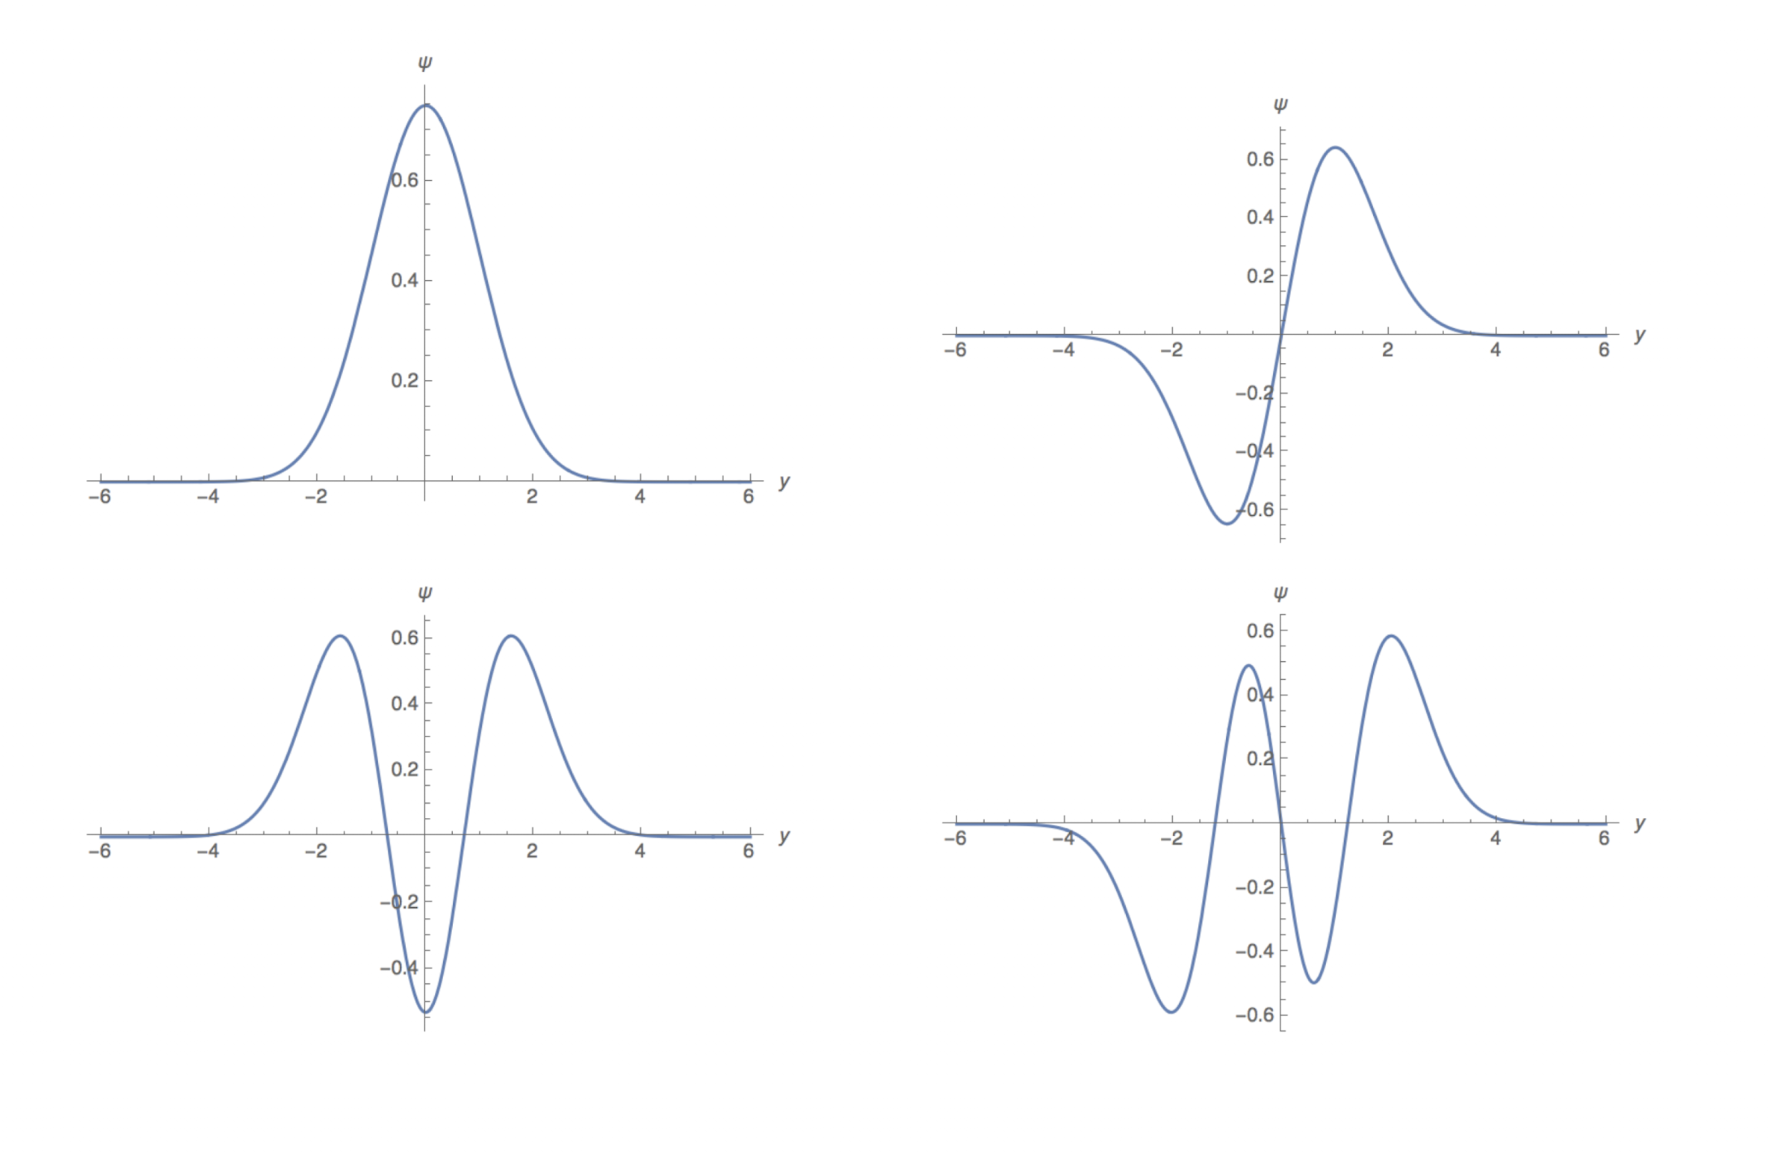
\includegraphics[width = 13cm]{waveOscillatore}	
\centering
\vspace{0.1in}
\caption{Funzione d'onda normalizzate. Scorrendo da sinistra verso destra si passa dallo stato fondamentale al terzo stato eccitato.}
\end{figure}

Notare come al crescere di $n$ crescono le intersezioni con l'asse delle ascisse da parte della funzione d'onda  $|n \rangle $, questo vuol dire che il valore medio dell'energia potenziale cresce con $n$ e analogamente l'energia cinetica.
\newpage
Quando il numero di zero di $|n \rangle$ aumenta, la curvature della funzione d'onda aumenta e quindi la derivata seconda assume dei valori sempre pi\`u grandi, da qui discende anche il fatto che l'energia  cinetica media aumenta. 

Se prendiamo valori molto grandi di $n$, abbiamo che la densit\`a di probabilit\`a $|\psi_n(x)|^2$ diventa molto grande per $x \simeq x_{max}$, dove $x_{max}$ coincide con il punto d'inversione (dove l'energia cinetica si annulla) di una particella nella trattazione classica dell'oscillatore armonico. Mediamente, una particella spende pi\`u tempo in un intorno dei punti d'inversione che al centro dell'intervallo $-x_{max} \leq x \leq x_{max}$.

 
\begin{figure}[!ht]
\vspace{0.1in}
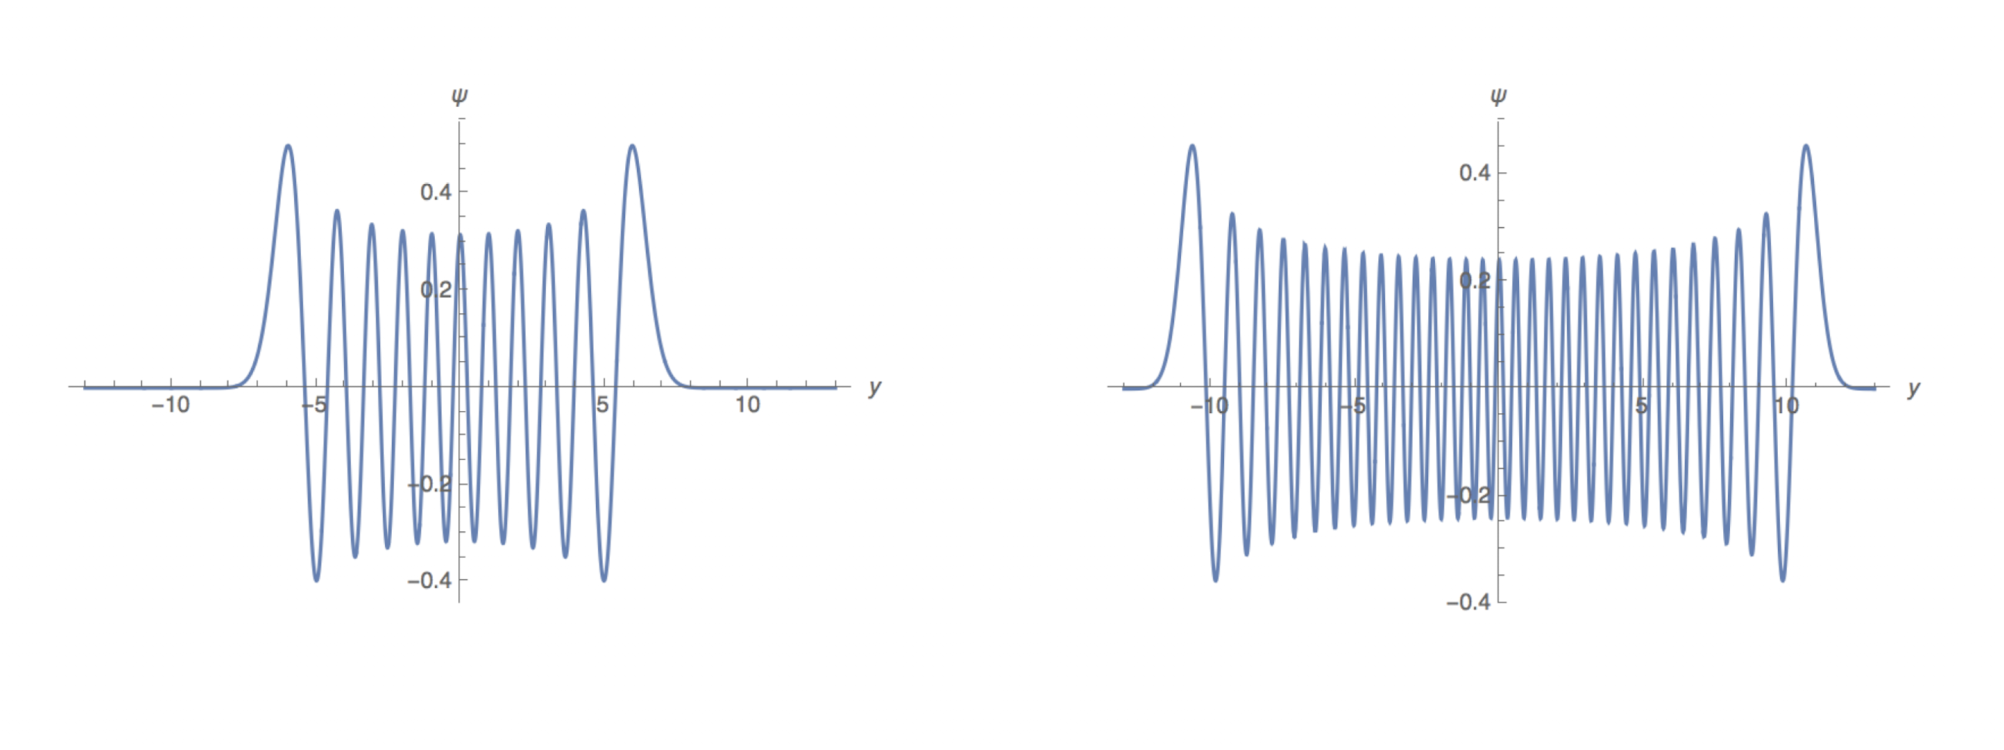
\includegraphics[width = 15cm]{waven}	
\centering
\vspace{0.1in}
\caption{Funzioni d'onda di un oscillatore armonico per il $20^{th}$} stato eccitato sulla sinistra, e il $60^{th}$ stato eccitato sulla destra.
\end{figure}

\subsubsection{Propriet\`a del polinomio di Hermite }

Il fatto che gli autostati soluzione dell'oscillatore armonico siano dati dal prodotto di un esponenziale e di un polinomio di Hermite, fa s\`i che queste funzioni siano invarianti rispetto alla trasformazione di Fourier. 
\begin{equation*}
	\psi(p) = e^{i \theta}\psi(x)|_{x = p /m\omega}
\end{equation*}
tale risultato fa s\`i che sotto trasformazione l'equazione di Schr\"odinger trasformata ci restituisce ancora l'equazione di un oscillatore armonico.

I polinomi Hermite sono funzioni o pari o dispari, infatti 
\begin{equation*}
	H_n(-\xi) = (-1)^n H_{n}(\xi)
\end{equation*}
tale propriet\`a ci permette, partendo dalle simmetrie del problema, di determinare la parit\`a o disparit\`a delle soluzioni. 

\section{Oscillatore armonico accoppiato}

Consideriamo una Hamiltoniana della forma 
\begin{equation*}
	H = \frac{p_1^2}{2m} + \frac{p_2^2}{2m} + \frac{m \omega^2}{2}(x_1^2 + x_2^2 + 2 \lambda x_1 x_2)
\end{equation*}

dove l'ultimo termine \`e una forma quadratica, di conseguenza esiste una matrice associata della forma 
\begin{equation*}
\left [ \begin{array}{cc}
		x_1 & x_2\\ 
	\end{array} \right ]
	\underbrace{\left [ \begin{array}{cc}
		1 & \lambda \\ 
		\lambda & 1 
	\end{array} \right ]}_{=Q}
	\left [ \begin{array}{c}
		x_1 \\ 
		x_2 
	\end{array} \right ] 
\end{equation*} 
dato che Q \`e una matrice simmetrica, questa risulta essere diagonalizzabile, ovvero esiste una matrice $R \in SO(3)$ tale per cui possiamo definire Q nel seguente modo 
\begin{equation*}
	Q = R^{T} \left [ \begin{array}{cc}
		q_1 & 0 \\ 
		0 & q_2 
	\end{array} \right ]R
\end{equation*} 
Per risolvere il problema riscriviamo l'equazione di Schr\"odinger dell'oscillatore armonico accoppiato rispetto ad una nuova base. Partendo da
\begin{equation}
	-\frac{\hbar^2}{2m} \left (\frac{\partial^2}{\partial x_1^2} + \frac{\partial^2}{\partial x_2^2} \right) \psi + V(x_1,x_2)\psi = E\psi 
\end{equation} 
definiamo i nuovi elementi della base facendo agire la matrice R $x' = Rx$ e in componenti diventa $x_k' = R_{ks}x_s$. La derivata parziale rispetto alle nuove coordinate diventa 
\begin{equation*}
	\frac{\partial }{\partial x_s} = \frac{\partial x'_k}{\partial x_s}\frac{\partial}{\partial x'_k} = R_{ks} \frac{\partial}{\partial x'_k}
\end{equation*}
in notazione vettoriale si ha che 
\begin{equation*}
	\nabla = R \;\nabla'
\end{equation*}
Riscrivendo (3.33) in forma vettoriale e utilizzando i risultati ottenuti si ha che
\begin{align*}
	&- \frac{\hbar^2}{2m} \nabla^2\psi + (\bold{x}^{T}Q\bold{x}) \psi = E \psi \\[0.5cm]
	&\iff - \frac{\hbar^2}{2m} \nabla^2\psi + (\bold{x}^TR^T\left [ \begin{array}{cc}
		q_1 & 0 \\ 
		0 & q_2 
	\end{array} \right ] \bold{x}R)\psi = E \psi \\[0.5cm]
	& \iff - \frac{\hbar^2}{2m} \left( \nabla' \right)^2 \psi + (\bold{x'}^T\left [ \begin{array}{cc}
		q_1 & 0 \\ 
		0 & q_2 
	\end{array} \right ] \bold{x'})\psi = E \psi
\end{align*}
dove per per il Laplaciano si \`e usata la relazione 
\begin{equation*}
	\nabla^2 = \nabla^T \cdot \nabla = (R\nabla')^T \cdot (R\nabla') = (\nabla')^TR^TR\nabla' = (\nabla')^2  
\end{equation*}
L'equazione di Schr\"odinger nel nuovo sistema di coordinate assume la forma 
\begin{equation*}
	- \frac{\hbar^2}{2m} \left ( \frac{\partial^2}{\partial x_1'^2 } + \frac{\partial^2}{\partial x_2'^2}\right) \psi  + \frac{m\omega^2}{2}\left ( (x_1')^2q_1 + (x_2')^2q_2 \right) \psi = E \psi
\end{equation*}
Studiando il polinomio caratteristico $P(q) = 0$ associato alla matrice (Q - qI) si dimostra che i termini $q_{1}$ e $q_2$ rappresentano le frequenze di oscillazione proprie del sistema.
\begin{equation*}
	det(Q-qI) = \text{det} \left [ \begin{array}{cc}
		1-q & \lambda \\
		\lambda & 1-q 
	\end{array} \right ] = (1-q)^2-\lambda^2 = 0 \Rightarrow q_{1,2} = 1 \pm \lambda
\end{equation*}
Determinato il loro valore esplicito e sostituendo nell'equazione di Schr\"odinger definita rispetto alla nuova base, abbiamo che la Hamiltoniana pu\`o essere interpretata come la somma di due Hamiltoniane che rappresentano rispettivamente un oscillatore armonico con una sua frequenza propria di oscillazione distinta.
\begin{equation*}
	H = H_1 + H_2 = \frac{p_1^2}{2m} + \frac{m\omega^2}{2}(x_1')^2(1+\lambda) + \frac{p_2^2}{2m} + \frac{m \omega^2}{2}(1-\lambda)
\end{equation*}
dove possiamo definire $\omega_1 = \omega \sqrt{1+\lambda}$ per la Hamiltoniana $H_1$ e $\omega_2 = \omega \sqrt{1 -\lambda }$ per la Hamiltoniana $H_2$. Gli autovalori associati al sistema, vista la natura additiva della Hamiltoniana del sistema complessivo, possono essere espressi nel seguente modo 
\begin{equation*}
	H |n \rangle = E_{n}|n \rangle \iff H_1|n\rangle + H_2|n\rangle = E_{n_1}|n \rangle + E_{n_2}|n \rangle  \Rightarrow E_n = E_{n_1} + E_{n_2}  
\end{equation*}
che usando i risultati della sezione precedente, analiticamente assumono la forma
\begin{align*}
	E_{n_1,n_2} = & \hbar \omega_1 \left (n_1 + \frac{1}{2} \right ) + \hbar \omega_2 \left (n_2 + \frac{1}{2} \right ) \\[0.5cm] = 
	& \hbar \omega \sqrt{1+\lambda} \left (n_1 + \frac{1}{2} \right ) + \hbar \omega \sqrt{1-\lambda}\left (n_2 + \frac{1}{2} \right )
\end{align*}

\subsection{Oscillatore armonico in un campo elettrico costante}

Consideriamo una particella di carica $q$ che si muove sotto l'azione di una forza centrale data da un potenziale elettrostatico 
\begin{equation*}
	V(x) = - q \varepsilon x
\end{equation*}
e da una forza di natura elastica, dunque la Hamiltoniana che descrive la dinamica del sistema \`e data da 
\begin{equation*}
	H = \frac{p^2}{2m} + \frac{m\omega^2}{2}x^2 - q\varepsilon x
\end{equation*}
riscriviamo la hamiltoniana nel seguente modo
\begin{equation*}
	H = \frac{p^2}{2m} + \frac{m \omega^2}{2} \left (x - \frac{q \varepsilon}{m \omega^2 }\right)^2 -\frac{q^2\varepsilon^2}{2m\omega^2}
\end{equation*}
effetuando un cambio di variabile
\begin{equation*}
	x' = x - \frac{q\varepsilon}{m \omega^2}
\end{equation*}
in modo tale da avere un oscillatore armonico centrato nell'origine.
\newpage 
\noindent Per quando discusso nei paragrafi precedenti sappiamo che l'energia dell'oscillatore armonico \`e quantizzata e in questo caso specifico, vista la presenza di una costante aggiuntiva nella Hamiltoniana, assume l'espressione 
\begin{equation*}
	E_n = \hbar \omega\left(n + \frac{1}{2} \right ) - \frac{q^2\varepsilon^2}{2m\omega^2}
\end{equation*}
le autofunzioni associate equivalgono a dei polinomi di Hermite traslati.
\begin{equation*}
	\psi_n(x) = Cost \; H_n \left (\alpha \left [x-\frac{q\varepsilon}{m\omega^2} \right ]  \right )e^{-\frac{\alpha^2}{2}\left (x-\frac{q\varepsilon}{m\omega^2} \right )^2} \quad \text{dove} \quad \alpha = \sqrt{\frac{m\omega}{\hbar}}
\end{equation*}
Ipotizziamo di effetuare une sperimento in cui al tempo $t = 0$ non \`e presente nessun campo elettrostatico $\varepsilon = 0$ e il sistema si trova nella configurazione di stato fondamentale $n = 0$ e dunque l'energia \`e al minimo possibile, in un istante  successivo $t > 0$ il campo elettrico viene acceso istantaneamente e quindi $\varepsilon \neq 0$. In condizioni di questo tipo possiamo domandarci: "\textit{Qual \`e la probabilit\`a che il sistema accoppiato resti nello stato fondamentale di partenza ?}
\newline

Per rispondere a questa domanda, ci ricordiamo che un generico stato di un sistema pu\`o essere espresso come combinazioni lineare delle autofunzioni della Hamiltoniana H, dato che queste costituiscono una base ortonormale di un sotto spazio di Hilbert.
\begin{equation*}
	\psi = \sum_{n} c_n \varphi_{n}
\end{equation*}  
Per determinare la probabilit\`a che il sistema di trovi ancora nello stato fondamentale una volta che $\varepsilon \neq 0$ \`e data dal prodotto
\begin{equation}
	|c_0|^2 = \left |\int dx \; (\varphi_0(x)^{\varepsilon \neq 0})^* \; \varphi_0(x)^{\varepsilon = 0} \right | ^2 = P(E = E_0)
\end{equation}
Dai risultati precedenti possiamo definire
\begin{align*}
	& \varphi_0 (x)^{\varepsilon = 0} = \left ( \frac{\alpha^2}{\pi}\right )^{1/4} e^{-\frac{\alpha^2}{2}x^2} \\[0.5cm]
	& \varphi_0(x)^{\varepsilon \neq 0} = \left ( \frac{\alpha^2}{\pi}\right )^{1/4} e^{\frac{\alpha^2}{2}\left (x- \frac{q\varepsilon}{m\omega^2}\right)^2}
\end{align*}
definiamo esplicitamente (3.34) 
\begin{align*}
	P(E=E_0) = &\left ( \frac{\alpha^2}{\pi}\right )^{1/2} \int_{\mathbb{R}}dx \; e^{\frac{\alpha^2}{2}\left (x- \frac{q\varepsilon}{m\omega^2}\right)^2}e^{\frac{\alpha^2}{2}\left (x- \frac{q\varepsilon}{m\omega^2}\right)^2} = \\[0.5cm]
	 = & \left ( \frac{\alpha^2}{\pi}\right )^{1/2} \int_{\mathbb{R}}dx \; e^{- \alpha^2 \left ( x - \frac{q\varepsilon}{2m\omega^2}\right)^2} e^{-\frac{\alpha^2}{2}\frac{q^2\varepsilon^2}{m^2\omega^4} + \frac{\alpha^2 q^2\varepsilon^2}{4m^2\omega^4}} = \\[0.5cm]
	 = & \left ( \frac{\alpha^2}{\pi}\right )^{1/2} \sqrt{\frac{\pi}{\alpha^2}} \; e^{-\frac{\alpha^2}{2}\frac{q^2\varepsilon^2}{m^2\omega^4} + \frac{\alpha^2 q^2\varepsilon^2}{4m^2\omega^4}} = e^{- \frac{\alpha^2}{4}\frac{q^2 \varepsilon^2}{m^2 \omega^4}}
\end{align*}

\section{Moto di una particella carica in un campo elettromagnetico}

Classicamente, la forza esercitata su una particella carica in un campo elettromagnetico \`e descritta dalla \textit{forza di Lorentz}:
\begin{equation*}
	\bold{F} = q(\bold{E} + \bold{v} \times \bold{B})
\end{equation*}
dove $q$ indica la carica e $\bold{v}$ la sua velocit\`a. Le velocit\`a dipendenti dalla forza di un campo magnetico sono leggermente differenti da quelle dovuti ad una forza conservativa data da una potenziale centrale, di conseguenza il passaggio dalla descrizione classica alla descrizione quantistica, sostituendo posizioni e momenti con gli opportuni operatori, risulta essere pi\`u delicato di quanto visto nelle casistiche precedenti.

\subsection{Descrizione classica di una particella in un campo}

Dato che la forza di Lorentz dipende dalla velocit\`a, non pu\`o essere espressa come gradiente del potenziale. Inoltre il cammino che compie la particella carica deve essere descrivibile dal principio di minima azione. Dato che $\bold{E}(\bold{r},t)$ e $\bold{B}(\bold{r},t)$ sono legate tra loro dalle equazioni di Maxwell, possiamo introdurre il potenziale scalare $U(\bold{r},t)$ e il \textit{potenziale vettore} $\bold{A}(\bold{r},t)$, in questo modo 
\begin{equation*}
	\left \{ \begin{array}{l}
		\bold{E}(\bold{r},t) = - \nabla U(\bold{r},t) - \frac{\partial}{\partial t}\bold{A}(\bold{r},t)\\[0.5cm]
		\bold{B}(\bold{r},t) = \nabla \times \bold{A}(\bold{r},t)
	\end{array}\right.
\end{equation*}
Quando effettuiamo una trasformazione di questo tipo, diciamo che si \`e effettuata una \textit{trasformazione di Gauge}. Notare che per una trasformazione di questo tipo il campo magnetico ed elettrico non sono univocamente determinati da $\bold{A}$ ed $U$, possiamo avere 
	valori differenti di $\bold{A}'$ e $U'$ che descrivono il medesimo campo.

Essendo la trasformazione di Gauge una ridondanza della descrizione fisica del campo elettromagnetico, poich\`e non \`e altro che una sua parametrizzazione mediante $\bold{A}$ e $U$ (che sono grandezze senza un reale significato fisico), si ha dunque che le grandezze fisiche dipendenti da tali quantit\`a restano invariate. Si dice che sia la meccanica classica che quella quantistica sono \textit{invarianti per Gauge}.
	
La  Lagrangiana corrispondente al sistema parametrizzato \`e data da
\begin{equation*}
	\mathcal{L} = \frac{1}{2}m \bold{v}^2 - qU + q\bold{v} \times \bold{A} 
\end{equation*}
per definire la Hamiltoniana del sistema definiamo i momenti canonici 
\begin{equation}
	p_i = \frac{\partial \mathcal{L}}{\partial \dot{x}_i} = mv_i + qA_i
\end{equation}
in cui compare un termine aggiuntivo al prodotto tra massa e velocit\`a. 
\newpage
 
Dato che la Hamiltoniana per definizione \`e la trasformata di Legendre della Lagrangiana si ha che
\begin{equation*}
	H(q_i,p_i) = \sum_{i}(mv_i + qA_i)v_i - \frac{1}{2}m\bold{v}^2+ qU - q \bold{v} \cdot \bold{A} =  \frac{1}{2}m\bold{v}^2 + qU 
\end{equation*}
che possiamo riscrivere in forma compatta rispetto ai momenti generalizzati come 
\begin{equation*}
	H = \frac{1}{2m}(\bold{p} - q \bold{A}(\bold{r},t))^2+ qU(\bold{r},t)
\end{equation*}
Consideriamo ora le equazioni di Hamilton del moto 
\begin{equation*}
	\left \{ \begin{array}{l}
		\dot{x}_i = \frac{\partial H }{\partial p_i} \\
		\dot{p}_i = -\frac{\partial H}{\partial x_i}
	\end{array}\right.
	\iff 
		\left \{ \begin{array}{l}
		\dot{x}_i = \frac{1}{m} (p_i - qA_i)\\
		\dot{p}_i = -\frac{1}{m}(p_j-qA_j)\left ( -q \frac{\partial A_j}{\partial x_i}\right)-q\frac{\partial U}{\partial x_i} = \frac{1}{m}\dot{x}_j \left (q \frac{\partial A_j}{\partial x_i} \right) - q \frac{\partial U}{\partial x_i}
	\end{array}\right.
\end{equation*}	
La prima equazione determina l'espressione per il momento canonico, mentre la seconda ci riconduce alla forza di Lorentz. Per capire in quale modo, procediamo nel calcolare la derivata prima dei momenti coniugati in (3.35):
\begin{align*}
	m\ddot{x}_i = & \; \dot{p}_i - \frac{d A}{d t} =  \dot{x}_j \left (q \frac{\partial A_j}{\partial x_i} \right) - q \frac{\partial U}{\partial x_i} - q \frac{\partial A}{\partial t} - q \frac{\partial A_i}{\partial x_j}\dot{x}_j = \\[0.5cm]
	= & \; - q \left ( \frac{\partial U}{\partial x_i} - \frac{\partial A_j}{\partial t} \right) + q \dot{x}_j \left (\frac{\partial A_j}{\partial x_i} - \frac{\partial A_i}{\partial x_j} \right) = \\[0.5cm]
	= & \; qE_i +q  \varepsilon_{ijk}\dot{x}_jB_k = qE_i + q (\dot{\bold{x}} \times \bold{B})
\end{align*}
In questo modo otteniamo l'espressione della forza di Lorentz.

\subsection{Descrizione quantistica di una particella in un campo}

Per passare alla trattazione quantistica, come sempre sostituiamo la quantit\`a di moto con la il suo analogo operatore $ \hat{\bold{p}} = - i \hbar \nabla $. In questo $\hat{p_i} \neq  m \hat{v}_i$, di conseguenza avremo che le velocit\`a in direzioni differenti non commutano. L'operatore associato all'osservabile della Hamiltoniana viene definito come 
\begin{equation*}
	\hat{H} = \frac{1}{2m} \left ( - i\hbar\nabla - q\bold{\hat{A}} \right)^2 - qU 
\end{equation*}
 L'operatore 
\begin{equation*}
	(\hat{p} - q \hat{A})^\dag = (\hat{p} - q \hat{A}) 
\end{equation*}
\`e un operatore autoaggiunto.
L'equazione di Schr\"odinger associata al sistema \`e definita nel seguente modo
\begin{equation}
	i\hbar \frac{\partial \psi }{\partial t} = \frac{1}{2m} (-i\hbar \nabla - qA)^2 \psi + qU\psi 
\end{equation}
L'equazione dipende dalla scelta dei potenziale vettoriale e del potenziale scalare, dove entrambi possono essere definiti arbitrariamente. Per questo motivo l'informazione restituita dall'equazione (3.36) deve essere invariante rispetto alla scelta di $A$ e $U.$ 
\newpage 

Per dimostrarlo partiamo dai parametri A e U e consideriamo la loro trasformazione 
\begin{equation}
	\left \{\begin{array}{l}
		U' = U - \frac{\partial \Lambda}{\partial t} \\ 
		A' =  A - \nabla \Lambda \\
	\end{array}\right.
\end{equation}

dove il termine $\Lambda$ prende il nome di \textit{funzione di Gauge}. Dalla seconda equazione avremo che il campo magnetico $\bold{B}$ rimane invariato, ma non quello elettrostatico $\bold{E}$, ma utilizzando la prima trasformazione in (3.37) ovviamo a questo problema. Dato che la Hamiltoniana dipende dal vettore potenziale $\bold{A}$ e quindi dipende dalla scelta del gauge, questo ci suggerisce che la funzione d'onda non \`e un invariante rispetto alla trasformazione. La corrispondente trasformazione \`e data da 
\begin{equation}
	\psi'(\bold{r},t) = \exp \left [i \frac{q}{\hbar} \Lambda(\bold{r},t) \right ]\psi(\bold{r},t)
\end{equation}

La trasformazione di gauge introduce un termine aggiuntino di fase alla funzione d'onda di partenza. Per dimostrare l'invarianza dell'equazione (3.36) osserviamo anche che i momenti $p_i$ sono invarianti rispetto alla trasformazione di gauge e introduciamo il risultato intermedio 
\begin{align*}
	(\hat{p}'_i - qA'_i)e^{\frac{i}{\hbar}q \Lambda } = & \;e^{\frac{i}{\hbar}q \Lambda}(\hat{p}_i-qA'_i) + [\hat{p}_i-qA_i,e^{\frac{i}{\hbar}q\Lambda}]  = \\[0.5cm]
	=& \; e^{\frac{i}{\hbar}q\Lambda}(\hat{p}_i-qA'_i) + q \frac{\partial \Lambda}{\partial x_i}e^{\frac{i}{\hbar}q\Lambda} = \\[0.5cm]
	= & \; e^{\frac{i}{\hbar}q\Lambda}\left (\hat{p}_i-qA'_i + q\frac{\partial \Lambda}{\partial x_i} \right) = e^{\frac{i}{\hbar}q\Lambda}(\hat{p}_i - qA_i)   
\end{align*}
Partendo dalla trasformazione della funzione d'onda (3.38) e sostituendola in (3.37) avremo che
\begin{align*}
	  & e^{\frac{i}{\hbar}q\Lambda} \left ( i \hbar \nabla - q \frac{\partial \Lambda}{\partial t}\right)\psi = \frac{1}{2m}e^{\frac{i}{\hbar}q\Lambda}(\hat{\bold{p}}-q\bold{A}'_i)^2 \psi + q e^{\frac{i}{\hbar}q\Lambda}\left ( U - \frac{\partial \Lambda}{\partial t}\right) \psi  \iff \\[0.5cm]
	  & \iff i \hbar \frac{\partial \psi}{\partial t} = \frac{1}{2m} (\hat{p} -qA)^2\psi +qU\psi
\end{align*}
e dunque l'equazione di Schr\"odinger risulta essere invariante per trasformazione di gauge.

Osserviamo  che il termine di fase introdotto in (3.38) sulla trasformazione della funzione d'onda non influisce sulla densit\`a di probabilit\`a, infatti
\begin{equation*}
	|\psi(\bold{r},t)|^2 =|\psi'(\bold{r},t)|^2
\end{equation*}
di conseguenza cambia l'espressione della funzione d'onda, ma rimane immutata l'informazione fisica contenuta.

\subsection{Particella in campo magnetico costante}

Consideriamo la Hamiltoniana 
\begin{equation*}
	H = \frac{1}{2m} (\bold{p}-q\bold{A})^2 + qU = \frac{1}{2m}\bold{p}^2 - \frac{q}{2m}(\bold{p} \cdot \bold{A} + \bold{A} \cdot \bold{p}) + \frac{q^2}{2m}\bold{A}^2 + qU
\end{equation*}
\newpage
scegliamo un gauge affinch\`e $\nabla \cdot \bold{A} = 0$, tale condizione in meccanica quantistica si traduce nel richiedere che 
\begin{equation*}
	\sum_{i}^3 [p_i,A_i] = - i \hbar \left ( \frac{\partial A_1}{\partial x_1} + \frac{\partial A_2}{\partial x_2} + \frac{\partial A_3}{\partial x_3}\right) = - i\hbar \nabla \cdot \bold{A} = 0
\end{equation*}
e quindi che $[\bold{p},\bold{A}] = 0$. La Hamiltoniana assume la forma 
\begin{equation}
	H = \frac{1}{2m} \bold{p}^2 -\frac{q}{m} \bold{p} \cdot \bold{A} + \frac{q^2}{2m}\bold{A} + qU
\end{equation}
Scegliamo un potenziale vettore $\bold{A}$ affinch\`e venga preservata la condizione sulla sua divergenza e il campo magnetico $\bold{B}$ resti costante, per farlo risolviamo il sistema di equazioni alle derivate parziali 
\begin{equation*}
	\left \{ \begin{array}{l}
		\bold{B} = \nabla \times \bold{A} \\
		\nabla \cdot \bold{A} = 0
	\end{array}\right.
\end{equation*}
che ha come soluzione  
\begin{equation*}
	\bold{A} = -\frac{1}{2} \bold{x} \times \bold{B}
\end{equation*}
Il prodotto scalare tra momenti coniugati e potenziale vettore presenti nella Hamiltoniana possono essere riscritti in funzione della soluzione, calcolando
\begin{equation*}
	\bold{p} \cdot \bold{A} = \sum_i p_iA_i = \sum_i\frac{1}{2}p_i \varepsilon_{ijk}x_jB_k = \sum_i\frac{1}{2} \varepsilon_{ijk}p_ix_jB_k = \sum_i \frac{B_k}{2}\varepsilon_{ijk}x_jp_i = \sum_k\frac{B_k}{2}(\bold{x} \times \bold{p})_{k} = \frac{1}{2} \;\bold{B} \cdot \bold{L}
\end{equation*}
e quindi ottenendo 
\begin{equation*}
	H = \frac{\bold{p}^2}{2m} - \frac{q}{2m}\bold{B} \cdot \bold{L} + \underbrace{\frac{q^2}{8m}|\bold{x} \times \bold{B}|^2}_{(I)} + qU
\end{equation*}
Se $\bold{B}$ \`e sufficientemente piccolo il termine (I) \`e trascurabile e quindi 
\begin{equation*}
	H = - \vec{\mu} \cdot \bold{B}
\end{equation*}
dove il termine $\vec{\mu}$ rappresenta il \textit{momento magnetico}. Ogni volta che una particella possiede un momento angolare, il momento magnetico fornisce un contributo al moto rotazionale dato che $\vec{\mu} = \gamma \bold{L}$, dove $\gamma$ \`e il \textit{fattore giromagnetico}.

Nella formulazione ridotta della Hamiltoniana (in cui trascuriamo (I)) abbiamo che il fattore giromagnetico coincide con $\gamma = q /2m$, per un elettrone vista la dipendenza dalla carica avremo che $\gamma <0$. Per eliminare la dipendenza dal segno della carica possiamo definire 
\begin{equation*}
	\mu_B = \frac{|q|\hbar}{2m}
\end{equation*}
che prende il nome di \textit{magnetone di Bohr}. Nel sistema internazionale la sua unit\`a di misura \`e data da $\mu_b \simeq 9 \times 10^-24 \;  J/T $.
\newpage 
\subsection{Effetto Zeemann}

Consideriamo un elettrone di una atomo idrogenoide, che si muove in un potenziale Coulombiano e in presenza di un campo magnetico costante, la Hamiltoniana che descrive la dinamica della particella \`e data dall'equazione (3.39). Tale Hamiltoniana possiamo rappresentarla come il contributo di tre Hamiltoniane
\begin{equation*}
	H = H_0 + H_1 + H_2
\end{equation*}
dove rispettivamente 
\begin{align*}
	& H_0 = \frac{\bold{p}^2}{2m} + qU \\[0.3cm]
	& H_1 = -\frac{q}{2m}\bold{B} \cdot \bold{L} \\[0.3cm]
	& H_2 = \frac{q^2}{8m}|\bold{x} \times \bold{B}|^2 
\end{align*}
Dove $H_1$ viene definito \textit{termine paramagnetico} e $H_2$ termine \textit{diamagnetico}. Se scegliamo l'orientazione campo magnetico lungo l'asse $z$ l'ultimo termine assume la forma
\begin{equation*}
	H_2 = \frac{q^2B^2}{8m}(x^2+y^2)
\end{equation*}
nel caso degli atomi idrogenoidi possiamo approssimare $\langle x^2 + y^2\rangle \simeq a_0^2$ dove $a_0$ \`e il raggio di Bohr, e $\langle L_z \rangle \simeq \hbar$, di conseguenza il rapporto tra 
\begin{equation*}
\frac{H_2}{H_1} \simeq 10^-6 \quad  B/T 
\end{equation*}
Per i campi ottenibili in laboratorio ($B \simeq 1  \; T$), gli elettroni rimangono legati all'atomo, di conseguenza il termine $H_2$ \`e trascurabile rispetto $H_1$. Se confrontiamo $H_1$ con il potenziale Coulombiano
\begin{equation*}
	\frac{eB\hbar/2m_e}{m_ec^2\alpha^2/2} = \frac{e\hbar}{(m_ec\alpha)^2} \simeq \frac{1}{2.3 \times 10^5} \;\frac{B}{T}
\end{equation*}
dove $\alpha = \frac{e^2}{4\pi \varepsilon_0} \frac{1}{\hbar c} \simeq \frac{1}{137}$ denota la costante di struttura fine; tale risultato ci dice che i termine $H_1$ contribuisce in piccola parte alla perturbazione della classica divisione dello spettro atomico. Considerando quanto discusso fin'ora e tenendo solo il contributo paramagnetico, per un Hamiltoniana "spinless" (definireno lo che cos'\`e lo spin nel capitolo successivo), questa assumer\`a la seguente espressione
\begin{equation}
	\hat{H} = \hat{H_0} + \frac{e}{2m}B_zL_z
\end{equation}
Dato che $[\hat{H}_o,L_z] = 0$, commutano tra loro gli autostati della Hamiltoniana imperturbata $\psi_{lmn}(\bold{r})= R_{n,l}\;(\bold{r})Y_{l}^{m}(\theta,\phi)$ sono anche autostati di $\hat{H}$ e quindi gli autovalori sono dati da 
\begin{equation}
	E_{n,l,m} = -\frac{E_I}{n^2} + m\mu_B B = -\frac{E_n}{n^2} + m\hbar\omega_L
\end{equation}
\newpage 

dove $\omega_L = \frac{eB}{2m}$ indica la \textit{frequenza di Larmor}. Il risultato ci dice che la presenza di un campo magnetico modifica il valore dei livelli di energia associati alla Hamiltoniana $H_0$ per la quale $\bold{B} = 0$, di conseguenza osserviamo un ulteriore divisione di ciascuno dei (2l+1) livelli di energia degeneri associati ad $l$ fissato, separati tra loro per un salto di energia costante $\hbar \omega_L$. Tale fenomeno prende il nome di \textit{effetto Zeemann}.

\begin{figure}[!ht]
\vspace{0.4in}
\includegraphics[width = 13cm]{zeemann}	
\centering
\vspace{0.3in}
\caption{Splitting dei livelli energetici per un elettrone in un campo magnetico costante.}
\end{figure}

\subsection{Livelli di Landau}

Consideriamo una particella carica libera di muoversi sotto l'azione di un campo magnetico costante $\bold{B}(\bold{r})$. Classicamente avremo che la forza di Lorentz esercitata su di essa \`e data da 
\begin{equation*}
	\bold{F} = q\bold{v} \times \bold{B}(\bold{r})
\end{equation*}
dove $\bold{v}$ \`e la velocit\`a della particella. Il moto della particella \`e ovviamente descritto dalla terza (o seconda) legge di di Newton
\begin{equation*}
	m \frac{d^2\bold{x}}{dt^2}= \bold{F}
\end{equation*}
Assumendo che la direzione del campo magnetico sia parallela all'asse $z$, risolvendo l'equazione del moto avremo che che leggi orarie nello spazio della particella sono date da 
\begin{align*}
	&x(t) =x_0 + \sigma \cos (\omega_ct - \varphi_0) \\[0.3cm]
	&y(t) = y_0 + \sigma \sin(\omega_ct - \varphi_0)\\[0.3cm]
	&z(t) = z_0 + v_{0z}t
\end{align*}
\newpage 


dove i termini $x_0,y_0,z_0,\sigma,\varphi_0$ e $v_{0z}$ sono sei parametri costanti determinati dalle condizioni iniziali; il termine $\omega_c$ \`e la \textit{frequenza del ciclotrone} e \`e data da:
\begin{equation*}
	\omega_c = -q \frac{B}{\mu}
\end{equation*}
Le equazioni del moto determinate determinano un moto elicoidale nello spazio, il cui centro \`e dato da $C_0 = C_0(x_0,y_0)$, velocit\`a angolare $\omega_c$ e fase iniziale $\varphi_0$

\begin{figure}[!ht]
\vspace{0.1in}
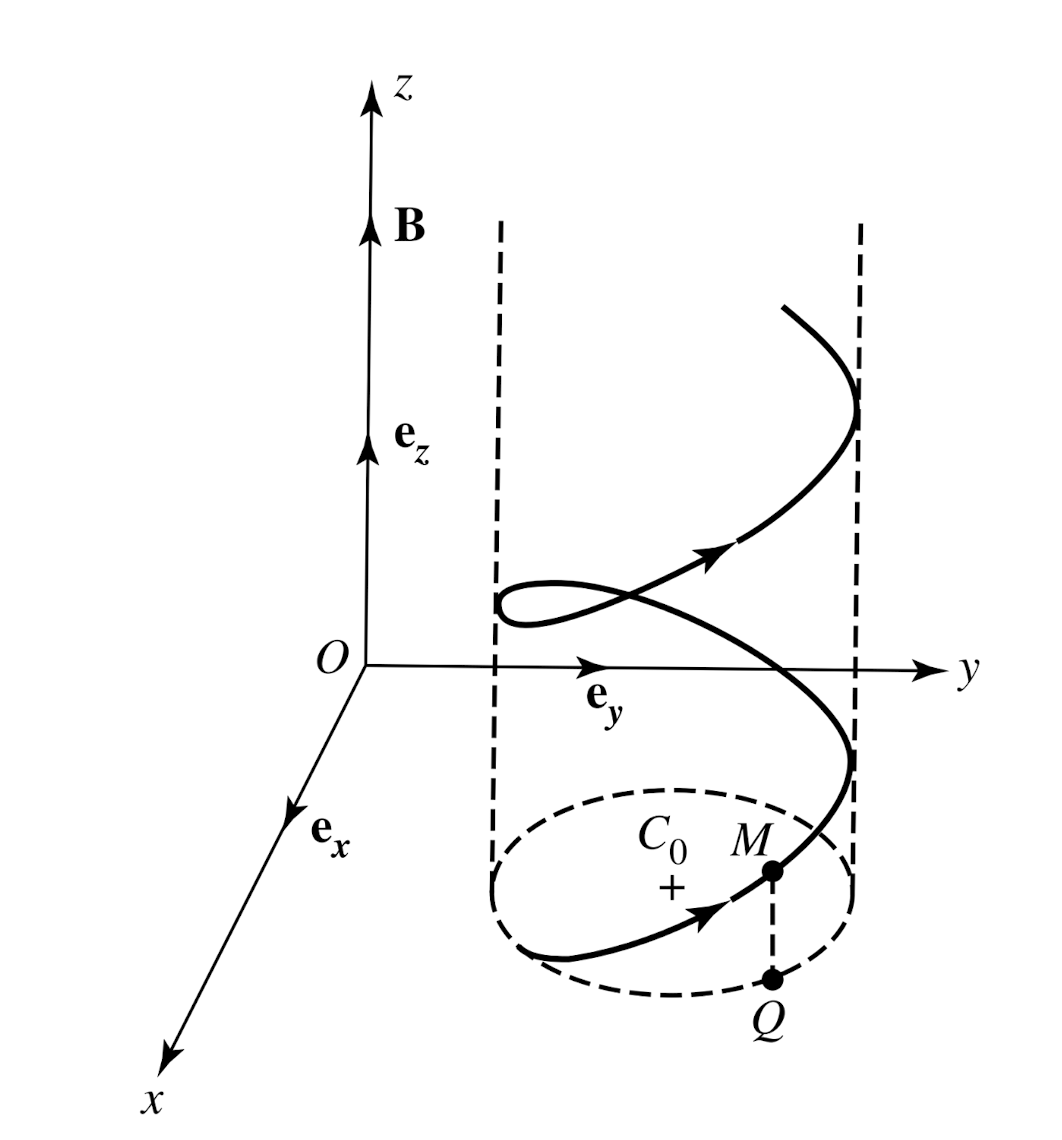
\includegraphics[width = 7cm]{elycoidal}	
\centering
\vspace{0.1in}
\end{figure}

Per descrivere il campo magnetico $\bold{B}(\bold{r})$, possiamo utilizzare il potenziale vettore $\bold{A}(\bold{r})$ legati tra loro dalla relazione 
\begin{equation*}
	\bold{B}(\bold{r}) = \nabla \times \bold{A}(\bold{r})
\end{equation*}
di conseguenza ripetendo i passaggi visti nelle sezioni precedenti possiamo definire la seguente Lagrangiana
\begin{equation*}
	\mathcal{L}(\bold{r},\bold{v}) = \frac{1}{2}m \bold{v}^2 + q \bold{v} \cdot \bold{A}
\end{equation*}
segue che i momenti coniugati $\bold{p}$ della posizione $\bold{r}$, si legano ad $\bold{A}$ e $\bold{v}$ secondo la relazione
\begin{equation*}
	\bold{p} = \nabla_{\bold{v}}\mathcal{L}(\bold{r},\bold{v}) = m \bold{v} + q \bold{A}(\bold{r})
\end{equation*}
Dunque la Hamiltoniana $H(\bold{r},\bold{p})$ \`e data da:
\begin{equation*}
	H(\bold{r},\bold{p}) = \frac{1}{2m}[\bold{p} - q \bold{A}]^2
\end{equation*}
Un gauge che pu\`o essere utilizzato \`e dato da $\bold{A} = -\frac{1}{2}(\bold{x} \times \bold{B})$, ma questo renderebbe l'equazione di Schr\"odinger pi\`u complicata. Una scelta pi\`u intelligente \`e considerare una direzione privilegiata nel piano (x,y), in questo modo l'equazione di Schr\"odinger coincide con quella di un oscillatore armonico. 

\newpage

Prendiamo un gauge $\bold{A} = (-By,0,0)$. Dato che $\bold{B}$ ha direzione lungo $z$, avremo che la Hamiltoniana diventa 
\begin{equation}
	\hat{H} = \frac{1}{2m}[(\hat{p}_x+qBy)^2 + \hat{p}^2_y + \hat{p}^2_z
\end{equation}
 In questo modo avremo che $\hat{H}$ commuta sia con $\hat{p}_x$ che con $\hat{p}_z$, di conseguenza avremo una base comune di autostati data da 
 \begin{equation*}
 	\psi(x,y,z) = e^{i/\hbar(p_x x+p_z z) }\chi(y)
 \end{equation*}
dove la funzione $\chi(y)$ \`e determinabile sostituendo la soluzione nell'equazione di Schr\"odinger 
\begin{align*}
	& \frac{1}{2m} [ (p_x +qBy)^2 + p_y^2 + p_z^2]\; \chi(y) = E \; \chi(y) \iff\\[0.5cm] 
	& \iff -\frac{p^2_y}{2m}\chi(y) + \frac{q^2B^2}{2m} \left (y + \frac{p_x}{qB} \right)^2\chi(y) + \frac{p_z^2}{2m}\chi(y) = E \; \chi(y) \iff \\[0.5cm]
	& \iff \left[\frac{{\hat{p_y}}^2}{2 m}+\frac{1}{2} m \omega^2\left(y-y_0\right)^2\right] \chi(y)=\left(E-\frac{\hat{p}_z^2}{2 m}\right) \chi(y) 
\end{align*}
dove $y_0 = -p_x / qB$ e $\omega_c$ \`e la frequenza ciclotronica della trattazione classica del moto della carica. Si osserva che il momento coniugato $p_x$ corrisponde alle coordiante del centro di un potenziale che definisce un oscillatore armonico lungo la direzione $y$ con frequenza $\omega_c$.  Di conseguenza, possiamo dedurre che gli autovalori della Hamiltoniana sono dati dati da una componente che descrive il moto libero della carica in direzione parallela al campo, e un insieme stati legati all'oscillatore armonico.
\begin{equation}
	E_{n,p_z} = \hbar \omega_c \left( n + \frac{1}{2} \right) + \frac{p_z^2}{2m}
\end{equation}
Il numero quantico $n$, definisce gli stati che prendono il nome di \textit{livelli di Landau}.

La soluzione dell'equazione di Schr\"odinger \`e data da
\begin{equation}
	 	\psi_{n,p_x,p_z}(x,y,z) = e^{i/\hbar(p_x x+p_z z) }\chi_n(y)\left(y + \frac{p_x}{qB} \right)
\end{equation}

osserviamo che il termine $p_z$ indicizza le autofunzioni, ma non rientra nel valore dell'energia, di conseguenza $p_x \in \mathbb{R}$. Questo vuol dire che esiste un continuo di funzioni d'onda che corrispondono allo stesso livello energetico.

Nelle righe precedenti abbiamo detto che che $p_x$ definisce il centro $y_0$ dell'oscillatore armonico, analiticamente questo \`e dato dalle relazioni
\begin{align*}
	&m\bold{\dot{x}} = \bold{p}-q\bold{A} \iff \bold{p} = m\bold{\dot{x}} + q \bold{A} \\[0.5cm]&\Rightarrow p_z = m\dot{x} - qBy \equiv  -qBy_0
\end{align*}
Il fatto che si abbia la direzione lungo $y$ \`e dato dal motivo che nel gauge si \`e scelta come direzione privilegiata. Se avessimo usato il gauge $\bold{A} = - \frac{1}{2}(\bold{x} \times \bold{B})$, l'equazione di Schr\"odinger avrebbe visto comparire due termini lungo $x$ e $y$ di oscillatore armonico accoppiati con un termine legato al momento angolare.

\noindent I livelli di Landau trovano una grande importanza nella trattazione quantistica dell'effetto Hall.

\section{Esempi ed Esercizi}

\subsection{Esercizio 1: Rotatore rigido}

Consideriamo una particella vincolata a muoversi su una sfera, la sua dinamica \`e descritta dalla Hamiltoniana 
\begin{equation*}
	H = \frac{1}{2I} \bold{L}^2
\end{equation*}
Determinare i valori dell'energia e la loro degenerazione.
\begin{proof}
Per quanto discusso nella sezione di teoria di questo capitolo sappiamo che le equazioni soluzione dell'equazione di Schr\"odinger sono date dalle armoniche sferiche $Y_{lm}(\theta, \phi)$, l'energia associata \`e data dai corrispettivi autovalori che rispetto all'operatore $\bold{L}^2$ sono dati da 
\begin{equation*}
	E_{l} = \frac{\hbar^2 l(l+1)}{2I}
\end{equation*}
per ciascun l fissato, abbiamo che $m = -l,...,0,...,l$ e dunque si hanno $2l+1$ stati associati al medesimo livello energetico.

\end{proof}

\subsection{Esercizio 2}

Consideriamo una particella nello stato iniziale 
\begin{equation*}
	|\psi(x,y,z) \rangle = \frac{\alpha^{\frac{5}{2}}}{\sqrt{\pi}} z e^{-\alpha \sqrt{x^2 + y^2 + z^2}} \quad\; \quad  \alpha > 0 
\end{equation*}
Determinare gli autovalori associati rispetto a $\bold{L}^2$ e $L_z$.
\begin{proof}
Riscriviamo lo stato di partenza rispetto alla basse formata dalla funzioni armoniche 
\begin{equation*}
	|\psi \rangle = C \; Y_{10}re^{-\alpha r} = f(r)Y_{10}(\theta,\phi)
\end{equation*}	
Rispetto ai due operatori abbiamo che 
\begin{equation*}
	\bold{L}^2|\psi \rangle = \hbar^2l(l+1)|_{l=1}|\psi \rangle  = 2 \hbar^2|\psi \rangle  \quad \; \quad L_z|\psi \rangle = \hbar m|_{m=0}|\psi \rangle = 0 
\end{equation*}

\end{proof}

\subsection{Esercizio 3}

Consideriamo una particella nel suo stato fondamentale vincolata in una buca sferica. Determinare la pressione esercitata sulle pareti.
\newpage

\begin{proof}
	La particella \`e soggetta ad un potenziale della forma 
	\begin{equation*}
		V(r) = \left \{ \begin{array}{l}
			0 \quad r \leq R \\
			\infty \quad r > R
		\end{array}\right.
	\end{equation*}
All'interno dell'equazione di Schr\"odinger dobbiamo tenere conto di un termine che descriva la componente del momento angolare della particella a cui \`e soggetta all'interno della buca sferica. Quindi
\begin{equation*}
	-\frac{\hbar^2}{2m}U''(r) + \left ( V(r) + \frac{\hbar^2 l(l+1)}{2mr^2}\right)U = EU
\end{equation*}
Gli stati della particella sono dati dalla soluzione dell'equazione che sono della forma 
\begin{equation*}
	|\psi \rangle = \frac{U(r)_{kl}}{r} Y_{lm}(\theta,\phi)
\end{equation*}
Per evitare problemi al contorno poniamo $U(r) = U(0) = 0$ in modo tale che $U(r) \in L^2(0,+\infty)$. Per richiesta dell'esercizio sappiamo che la particella \`e nel suo stato fondamentale, dunque $l = 0$ e l'equazione di Schr\"odinger diventa
\begin{equation*}
	-\frac{\hbar^2}{2m}U'' = EU \quad r < R
\end{equation*}
che coincide son le equazioni di una particella in una buca infinita, le soluzioni dell'equazione sono date da 
\begin{equation*}
	U_{n0} = \sqrt{\frac{2}{R}} \sin \left( \frac{n\pi r}{R}\right) \quad ; \quad E_{n} = \frac{n^2 \pi^2 \hbar^2}{2mR^2}
\end{equation*} 
Per lo stato fondamentale avremo che $n=1$ e dunque 
\begin{equation*}
		U_{10} = \sqrt{\frac{2}{R}} \sin \left( \frac{\pi r}{R}\right) \quad ; \quad E_{1} = \frac{ \pi^2 \hbar^2}{2mR^2}
\end{equation*}
La forza esercitata dalla particella sulle pareti della buca \`e data da
\begin{equation*}
	F = - \frac{dE_1}{dR} = \frac{\pi^2 \hbar^2}{mR^3} 
\end{equation*}
e quindi la pressione data dal rapporto della forza per unit\`a di superficie \`e equivalente a 
\begin{equation*}
	p = \frac{F}{4\pi R^2} =  \frac{\pi \hbar^2}{4mR^5}
\end{equation*}

\end{proof}

\subsection{Esercizio 4: Effetto Kasimir}

Consideriamo una particella vincolata in una buca sferica di raggio R definita dal  potenziale 
\begin{equation*}
	V(r) = \left \{ \begin{array}{l}
		-V_0 \quad r \leq R \\
		\infty \quad r > R
	\end{array}\right.
\end{equation*} 
\newpage

Per $V_0 > 0$. Trovare il minimo valore di $V_0$ per cui esiste almeno uno stato legato.

\begin{proof}
	Analogamente all'esercizio precedente l'equazione di Schr\"odinger \`e 
\begin{equation*}
	-\frac{\hbar^2}{2m}U''(r) + \left ( V(r) + \frac{\hbar^2 l(l+1)}{2mr^2}\right)U = EU
\end{equation*}	 
Se esiste almeno uno stato legato ci aspettiamo che sia per $l = 0$ e livelli energitici in cui $0 >-E>-V_0$ quindi
\begin{align*}
	& -\frac{\hbar^2}{2m}U''(r)  -V_0 U = EU \quad r < R\\[0.5cm] 
	& -\frac{\hbar^2}{2m}U''(r)  = EU \quad r > R
\end{align*}
Per $r > R$ abbiamo $U = e^{\pm \rho r}$ e per $r < R$ si ha $U(r) = e^{\pm ikr}$ soluzioni delle equazioni precedenti. Gli autovalori associati sono dati da 
\begin{equation}
	E = - \frac{\hbar^2 \rho^2}{2m} \quad ; \quad 
	 E + V_0 = \frac{\hbar^2k^2}{2m}
\end{equation}
Imponendo le condizioni al contorno, dove $U(0) = 0$ avremo che 
\begin{align*}
	U_I(r) = & \; A'e^{ikr} + A''e^{-ikr} = C \cos(kr) + D\sin(kr)  \quad r \leq R \\[0.5cm]
	 & \; \text{Se} \quad  U(0) = 0 \quad  \Rightarrow \quad U_I(r) = D\sin(kr)
\end{align*}
analogamente avremo 
\begin{equation*}
U_{II}(r) = Be^{- \rho r} \quad r > R	
\end{equation*}
Utilizzando le condizioni di raccordo sulla derivata prima definiamo il sistema di equazioni 
\begin{equation*}
	\left \{ \begin{array}{l}
		U_{I}(R) = U_{II}(R) \\
		U_{I}'(R) = U_{II}'(R)
	\end{array}\right. \quad \iff \quad 
	\left \{ \begin{array}{l}
		A \sin(kR) = Be^{-\rho R} \\
		kA \cos(kR) = -\rho Be^{-\rho R}
	\end{array}\right.
\end{equation*}
Dividendo membro a membro abbiamo che 
\begin{equation*}
	\frac{\tan(kR)}{k} = - \frac{1}{\rho} 
\end{equation*}
Dalle relazioni definite in (3.45) otteniamo la relazione $k^2 + \rho^2 = \frac{2mV_0}{\hbar^2}$ e dunque possiamo riscrivere l'uguaglianza precedente come
\begin{equation*}
	\tan(kR) = \underbrace{\frac{-k}{\left [ \frac{2mV_0}{\hbar^2} - k^2\right]^{1/2}}}_{=g(k)}
\end{equation*}
tale equazione non pu\`o essere risolte per via analitica e dunque ricorriamo al metodo grafico.
\newpage
 
\begin{figure}[!ht]
\vspace{0.1in}
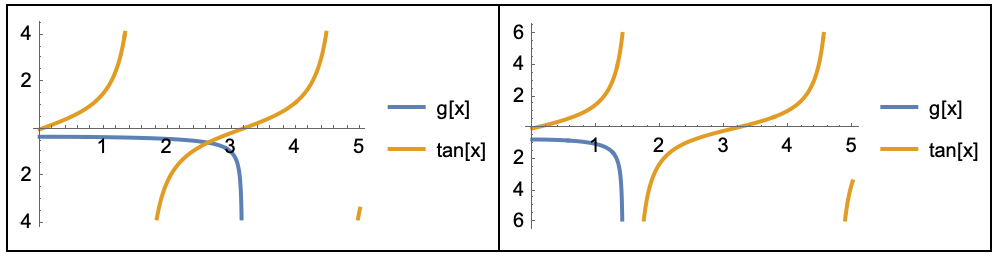
\includegraphics[scale = 0.8]{kasimir}	
\centering
\vspace{0.1in}
\caption{}
\end{figure}
In figura abbiamo le due casistiche in cui \`e possibile avere o non avere uno stato legato. Se prendiamo 
\begin{equation*}
	\sqrt{\frac{2mV_0}{\hbar^2}} \geq \frac{\pi}{2R}
\end{equation*}
avremo che la funzione $g(k)$ interseca la funzione tangente in almeno un punto, come si osserva nel primo grafico in figura 3.6. Quindi per rispondere alla domanda del problema, avremo che il valore minimo del potenziale per avere uno stato legato \`e dato da 
\begin{equation*}
	V_0 \geq  \frac{\pi^2 \hbar^2}{8mR^2}
\end{equation*}

\end{proof}

\subsection{Esercizio 5}

Consideriamo una particella di massa $m$ soggetta ad un potenziale elastico e la cui dinamica \`e descritta dalla Hamiltoniana di un oscillatore armonico con frequenza $\omega$. Si trova nello stato iniziale
\begin{equation*}
	\psi(x) = \mathcal{N} \left( 1 + \frac{\alpha x}{2}\right)e^{-\frac{\alpha^2 x^2}{2}} \quad \text{dove} \quad \alpha = \sqrt{\frac{m \omega}{\hbar}} 
\end{equation*}
Determinare:
\begin{enumerate}
	\item La probabilit\`a associata agli stati energetici possibili della configurazione iniziale.
	\item L'evoluto temporale del valore medio della posizione $\langle x \rangle (t)$.
\end{enumerate}

\begin{proof}
1) Per un oscillatore armonico le funzioni soluzione dell'equazione e i rispettivi autovalori sono dati da 
\begin{equation*}
	|n \rangle = \left( \frac{\alpha^2}{\pi} \right)^{\frac{1}{4}} \frac{H_n(\alpha x)}{\sqrt{n!2^n}}e^{-\frac{\alpha^2 x^2}{2}} \quad ; \quad E_n = \hbar \omega \left ( n + \frac{1}{2}\right) \quad n \in \mathbb{N}
\end{equation*}
Riscriviamo la funzione d'onda iniziale rispetto alla base $\varphi_n$, prendendo
\begin{equation*}
	\varphi_0 = C e^{-\frac{\alpha^2 x^2}{2}} \quad \; \quad \varphi_1 = C \; \frac{2 \alpha x}{\sqrt{2}}e^{- \frac{\alpha^2x^2}{2}}
\end{equation*}
\newpage

\begin{equation*}
	\psi(x) = cost \left ( \varphi_0 + \frac{\varphi_1}{2\sqrt{2}}\right) = \sqrt{\frac{8}{9}} \left ( \varphi_0 + \frac{\varphi_1}{\sqrt{8}}\right)
\end{equation*}
La probabilit\`a per gli stati energetici possibili \`e data da 
\begin{equation*}
	P(E=E_0) = \frac{8}{9} \quad \text{e} \quad P(E=E_1) = \frac{1}{9}
\end{equation*}
2) Per calcolare il valore medio della posizione nel tempo, applichiamo  l'operatore di evoluzione temporale 
\begin{equation*}
	\psi(x,t) = \sqrt{\frac{8}{9}} \left (  \varphi_0 e^{-\frac{i}{\hbar}E_0t} + \frac{1}{\sqrt{8}} \varphi_1e^{-\frac{i}{\hbar}E_1t}\right) = \sqrt{\frac{8}{9}} \left ( \varphi_0 e^{-\frac{i\omega t}{2}} + \frac{1}{\sqrt{8}}\varphi_1 e^{-i \frac{3 \omega t}{2}}\right)
\end{equation*}
quindi
\begin{align*}
	\langle x \rangle (t) = & \; \langle \psi |x |\psi \rangle = \int_{\mathbb{R}}dx \;  \psi^*(x,t) \; x \;\psi(x,t)  = \\[0.5cm]
	 = & \frac{8}{9} \int dx \; \left( \frac{1}{\sqrt{8}} e^{-i \omega t}x \; \varphi_0(x)\varphi_1(x) + \frac{1}{\sqrt{8}} e^{i \omega t}x \; \varphi_0(x) \varphi_1(x)\right) = \\[0.5cm] 
	 = & \frac{1}{9 \sqrt{8}}  \; 2 \cos(\omega t) \int_{\mathbb{R}}dx \; x\varphi_0(x) \varphi_1(x) = \frac{4}{9 \alpha} \cos(\omega t)
\end{align*}
dove abbiamo posto a zero i termini $\int dx \; \varphi_0 x \varphi_0$ per parit\`a.

\end{proof}

\subsection{Esercizio 6}

Calcolare i valori medi di posizione $\langle x \rangle $ e momenti $\langle p \rangle$ e le relative incertezze $\Delta x, \Delta y$, per uno stato stazionario dell'oscillatore armonico.
\begin{proof}
Consideriamo i seguenti operatori di posizione e momento
\begin{equation*}
	x = \sqrt{\frac{\hbar}{2m \omega}}(a+a^{\dag}) \quad ; \quad p = i \sqrt{\frac{m\hbar \omega}{2}}(a^{\dag}-a)
\end{equation*}	
Gli stati sono indicizzati da un intero 
\begin{equation*}
	|n \rangle = \frac{(a^{\dag})^n}{\sqrt{n!}}|0 \rangle 
\end{equation*}
per cui valgono le relazioni
\begin{equation*}
	\left \{ \begin{array}{l}
		a^{\dag}|n \rangle = \sqrt{n+1}|n+1 \rangle \\[0.3cm]
		a |n \rangle = \sqrt{n} |n-1 \rangle 
	\end{array}\right.
\end{equation*}
La posizione media \`e data 
\begin{equation*}
	\langle x \rangle = \langle n| x | n \rangle = \sqrt{\frac{\hbar}{2m \omega}} \langle n|a+a^{\dag}|n\rangle =
\end{equation*}
\newpage
\begin{equation*}
	=\sqrt{\frac{\hbar}{2m \omega}}(\langle n|n-1 \rangle \sqrt{n} + \langle n |n+1 \rangle \sqrt{n+1}) = 0
\end{equation*}
Il momento invece 
\begin{equation*}
	\langle p \rangle = \langle n|p|n \rangle = i \sqrt{\frac{m \hbar \omega}{2}} \langle n|a^{\dag} -a|n\rangle = 0
\end{equation*}
Infinite calcoliamo
\begin{align*}
	\langle x^2 \rangle = & \langle n| x^2|n\rangle  = \frac{\hbar}{2m \omega} \langle n| (a+a^{\dag})^2|n\rangle = \frac{\hbar}{2m \omega} \langle n| a^2 + a^{2 \dag} + aa^{\dag} +a^{\dag}a|n\rangle  = \\[0.5cm]
	 = &  \frac{\hbar}{2m \omega} \langle n| aa^{\dag} + a^{\dag}a |n \rangle = \frac{\hbar}{m \omega} \left (n + \frac{1}{2} \right ) 
\end{align*}
e analogamente
\begin{equation*}
	\langle p^2 \rangle = m \hbar \omega \left( n + \frac{1}{2}\right)
\end{equation*}
L'incertezza su momenti e posizioni
\begin{equation*}
	\Delta p^2 = \langle n| p^2|n \rangle = \langle p^2\rangle \quad ; \quad \Delta x^2 = \langle n |x^2|n\rangle = \langle x^2\rangle  
\end{equation*}
Verifichiamo il principio d'indeterminazione  di Heisenberg 
\begin{equation*}
	\Delta x \Delta p = \sqrt{\frac{\hbar}{2m}} \sqrt{m\hbar \omega}\left( n + \frac{1}{2}\right) = \hbar \left(n + \frac{1}{2}\right) \geq \frac{\hbar}{2}
\end{equation*}
Per $n=0$ si ha lo stato stazionario che corrisponde allo stato fondamentale dell'atomo d'idrogeno, in particolare lo stato d'indeterminazione \`e saturato.

\end{proof}

\subsection{Esecizio 7}

Consideriamo una particella di massa $m$ soggetta a un potenziale elastico. La sua evoluzione \`e descritta dall'oscillatore armonico e si trova in uno stato iniziale 
\begin{equation*}
	|\psi(0) \rangle = c_0|0\rangle + c_1|1\rangle 
\end{equation*}
Determinare 
\begin{enumerate}
	\item i coefficienti dello stato iniziale sapendo che $\langle H \rangle = \hbar \omega$ e $\langle x \rangle = \frac{1}{2} \sqrt{\frac{\hbar}{m \omega}}$.
	\item l'evoluto temporale della posizione media nel tempo $\langle x \rangle (t)$.
\end{enumerate}

\begin{proof}
	1) Sappiamo che $P(E=E_0) = |c_0|^2$ e $P(E =E_1)=|c_1|^2$ di conseguenza l'energia media \`e data da 
	\begin{equation*}
		\langle H \rangle = \sum_{n}E_nP(E=E_n) = |c_0|^2E_0 + |c_1|^2E_1 
	\end{equation*}
	e quindi
	\begin{equation*}
		\langle E \rangle = \frac{\hbar \omega}{2}(|c_0|^2+3|c_1|^2) = \hbar \omega
	\end{equation*}
\newpage
poich\`e lo stato sia normalizzato deve valere la condizione $|c_0|^2 + |c_1|^2 =1$. Sostituendo nell'equazione precedente abbiamo che 
\begin{equation*}
	|c_1|^2 = \frac{1}{2} \quad \; \quad |c_0|^1 = \frac{1}{2}
\end{equation*}
Dato che \`e presente un modulo il valore delle costanti \`e definito a meno di un termine di fase e quindi lo stato iniziale in forma generale \`e dato da
\begin{equation*}
	|\psi(0) \rangle = \frac{1}{\sqrt{2}}(e^{i\phi_1}|0 \rangle + e^{i \phi_2}|1\rangle)
\end{equation*}
In meccanica quantistica dato uno stato $|\tilde{\psi} \rangle = e^{i\alpha}|\psi\rangle $ moltiplicato per un numero complesso di modulo 1, la probabilit\`a intrinseca allo stato non cambia. In questo modo \`e possibile cambiare a piacimento le fasi.

2) Definiamo lo stato iniziale come
\begin{equation*}
	|\psi(0) \rangle = \frac{1}{\sqrt{2}}(|0\rangle + e^{i\phi}|1\rangle )
\end{equation*}
e procediamo a calcolare il valore medio della posizione rispetto allo stato iniziale
\begin{align*}
	& \langle x \rangle = \langle \psi(0) |x| \psi(0) \rangle = \frac{1}{2} [\langle 0|x|0\rangle + \langle 1 |x|1\rangle + e^{-\phi}\langle 1|x|0\rangle + e^{i\phi}\langle 0 |x|1\rangle ] = (*) \\[0.5cm]
	& \langle 1|x|0 \rangle = \sqrt{\frac{\hbar}{2m \omega}} \langle 1|a+a^{\dag}|0 \rangle  = \sqrt{\frac{\hbar}{2m \omega}}  \\[0.5cm]
	& \langle 0 |x|1 \rangle = \langle 1|x|0 \rangle^* = \sqrt{\frac{\hbar}{2m \omega}}  \\[0.5cm]
	& (*) = \sqrt{\frac{\hbar}{2m \omega}} \frac{1}{2} (e^{i\phi}+e^{-i\phi}) = \sqrt{\frac{\hbar}{2m \omega}}  \cos(\phi) = \frac{1}{2}\sqrt{\frac{\hbar}{2m \omega}}  \Rightarrow \phi = \frac{\pi}{4}
\end{align*}
quindi lo stato iniziale \`e dato da 
\begin{equation*}
	|\psi(0)\rangle = \frac{1}{\sqrt{2}}(|0\rangle + e^{i \frac{\pi}{4}}|1 \rangle )
\end{equation*}
applicando l'operatore di evoluzione temporale, avremo che il valore medio della posizione al tempo $t$ \`e dato da 
\begin{equation*}
	 \langle x \rangle(t) = \sqrt{\frac{\hbar}{2m \omega}}\cos(\omega t - \frac{\pi}{4}) 
\end{equation*}
Si ottiene una soluzione classica del moto perch\`e l'equazione dei valori medi coincide con quella classica.

\end{proof}


\setcounter{chapter}{3}
\chapter{Spin, Momento Angolare e Particelle Identiche}

\section{Teoria generale del momento angolare}
Nella seguente sezione introdurremo alcune proprier\`a generali che valgono per un momento angolare qualsiasi, e che quindi possono essere estese allo Spin di una particella che introdurremo nella sezione successiva.
\newline

\noindent Nel capitolo precedente abbiamo visto che $[L_i,L_j] = i\hbar \varepsilon_{ikk}L_k$ e $[\bold{L}^2,L_i] = 0 \; \forall i$. Inoltre scegliendo per convenzione $L_z$, dato che questa commuta con $\bold{L}^2$ hanno in comune un insieme di autofunzioni con i rispettivi autostati.
\begin{align*}
	&\bold{L}^2Y_{l}^{m} = \hbar^2 l(l+1)Y_{l}^{m} \quad l \in \mathbb{Z}^+\\[0.3cm]
	&L_{z}Y_{l}^{m} = \hbar m \quad m=-l,-l+1,...,l-1,l
 \end{align*}
Vogliamo definire degli operatori generalizzati di momento angolare che condividano le stesse propriet\`a. Per questo motivo definiamo l'operatore $\bold{J}$ costituitato un insieme di osservabili $J_x,J_y$ e $J_z$ che soddisfano le condizioni: 
\begin{align*}
	& [J_x,J_y] = i\hbar J_z \\[0.3cm]
	& [J_y,J_z] = i \hbar J_x \\[0.3cm]
	& [J_z,J_x] = i \hbar J_y 
\end{align*}
e introduciamo anche l'operatore 
\begin{equation*}
	\bold{J}^2 = J_x^2 + J_y^2 +J_z^2
\end{equation*}
Tale operatore \`e Hermitiano, dato che lo sono le sue componenti. E assumiamo che sia un osservabile. Vogliamo che l'operatore $\bold{J}^2$ commuti con tutte le sue componenti ovvero che 
\begin{equation*}
	[\bold{J}^2,J_i] = 0 \quad \forall i=x,y,z
\end{equation*}
\newpage
Come fatto nel caso del momento angolare, prendiamo per convenzione $J_z$ e cerchiamo una base comune di autostati a $\bold{J}^2$.
\begin{equation*}
	\left \{ \begin{array}{l}
		\bold{J}^2|j,m \rangle = \hbar^2(j+1)j|j,m \rangle \\[0.3cm]
		J_z|j,m\rangle = \hbar m |j,m \rangle 
	\end{array}\right.
\end{equation*}

\subsection{Operatori $J_+$  e $J_{-}$}

Al posto di utilizzare le componenti $J_x$ e $J_y$ del momento angolare generalizzato $\bold{J}$, \`e pi\`u conventi introdurre un operatore che \`e dato dalla loro combinazione lineare.
\begin{align}
	J_+ = J_x + i J_y \\[0.3cm]
	J_- = J_x - i J_y
\end{align}
analogamente a quanto fatto per la trattazione dell'oscillatore armonico dove abbiamo introdotto $a$ e $a^\dag$. Gli operatori $J_{+}$ e $J_{-}$ non sono Hermitiani  dato che 
\begin{equation*}
	J_+^\dag = J_-
\end{equation*}
discendenza diretta dal fatto che sono combinazione lineare di osservabili. I seguenti operatori soddisfano le operazioni  di commutazione nel seguente modo:
\begin{align*}
& [J_z,J_+] = \hbar J_+ \\[0.3cm]
& [J_z,J_-] = - \hbar J_{-} \\[0.3cm]
& [J_+,J_-] = 2 \hbar J_{z} \\[0.3cm]
& [ \bold{J}^2,J_{-}] = [\bold{J^2},J_{-}] = [\bold{J}^2,J_z] = 0
\end{align*}
e calcoliamo il prodotto tra i due operatori, che non commutando \`e differente a seconda dell'ordine di prodotto.
\begin{equation}
\begin{aligned}
J_{+} J_{-} & =\left(J_x+i J_y\right)\left(J_x-i J_y\right) \\
& =J_x^2+J_y^2-i\left[J_x, J_y\right] \\
& =J_x^2+J_y^2+\hbar J_z \\
J_{-} J_{+} & =\left(J_x-i J_y\right)\left(J_x+i J_y\right) \\
& =J_x^2+J_y^2+i\left[J_x, J_y\right] \\
& =J_x^2+J_y^2-\hbar J_z
\end{aligned}
\end{equation}
che possiamo riscrivere in modo compatto come 
\begin{equation}
\begin{aligned}
& J_{+} J_{-}=\mathbf{J}^2-J_z^2+\hbar J_z \\
& J_{-} J_{+}=\mathbf{J}^2-J_z^2-\hbar J_z
\end{aligned}
\end{equation}
\newpage
sommando i risultati in (4.4) definiamo
\begin{equation*}
	\mathbf{J}^2=\frac{1}{2}\left(J_{+} J_{-}+J_{-} J_{+}\right)+J_z^2
\end{equation*}

\subsection{Spettro di $\bold{J}^2$ e $J_z$}

\begin{theorem}[Porpriet\`a degli autovalori di $\bold{J}^2$ e $J_z$]
Se $j(j+1)\hbar^2$ e $m\hbar$ sono autovalori di $\bold{J}^2$ e $J_z$ associati al medesimo autovalore $|k,j,m \rangle$, allora $j$ e $m$ soddisfano la disuguaglianza:
\begin{equation*}
	- j \leq m \leq j
\end{equation*}	
\end{theorem}
\begin{proof}
 Consideriamo i vettori $J_+|k,j,m \rangle$ e $J_-|k,j,m \rangle$, e il quadrato della norma \`e dato da 
 \begin{align*}
 	\|J_+|k,j,m \rangle \|^2 = & \; \langle k,j,m|J_-J_+ |l,j,m \rangle = \langle k,j,m|\bold{J}^2-J_z^2-\hbar J_z |k,j,m\rangle = \\[0.5cm]
 	= &\hbar^2[j(j+1)-m^2-m)\langle k,l,m|k,l,m\rangle = \hbar^2(j-m)(j+m+1) \geq 0
 \end{align*} 
 con calcoli analoghi
 \begin{equation*}
 	\|J_-|k,j,m \rangle \|^2 = \hbar^2(j+m)(j-m+1) \geq 0
 \end{equation*}
 Se consideriamo $j$ fissato, otteniamo dei polinomi quadratici in $m$, se il coefficiente associato al termine quadrato \`e negativo la disuguaglianza \`e soddisfatta per $m$ in un intervallo chiuso $[-j,j+1]$. Per entrambe le equazioni avremo che 
 \begin{equation*}
 	-(j+1) \leq m \leq j \quad \text{e} \quad -j \leq m \leq j+1
 \end{equation*}
 dalla intersezione delle due condizioni deduciamo la tesi del teorema.
 
\end{proof}

\begin{theorem}[Propriet\`a de; vettore $J_+|k,l,m \rangle $]
	Sia $|k,l,m \rangle $ un autovettore $\bold{J}^2$ e $J_z$ con autovalori $j(j+1)\hbar^2$ e $m\hbar$.
	\begin{enumerate}
		\item Se $m=j$ allora $J_+|k,j,m \rangle = 0$
		\item Se $m < j$, allora $J_+|k,j,m \rangle$ \`e un autovettore di $\bold{J}^2$ e $J_z$ con autovalori $j(j+1)\hbar^2$ e $(m+1)\hbar$.
	\end{enumerate}
\end{theorem}

\begin{proof}
	2) Consideriamo $m <j$, dato che $J_+|k,j,m \rangle  \neq 0$, dimostriamo che \`e un autovettore di $\bold{J}^2$ e $J_z $. Dato che 
	\begin{equation*}
		[\bold{J}^2,J_+] |k,j,m \rangle = 0 \iff \bold{J}^2J_+|k,j,m \rangle = J_+\bold{J}^2|k,j,m \rangle = j(j+1)\hbar^2 J_+|k,j,m \rangle
	\end{equation*}	
avremo che $J_+|k,j,m \rangle$ \`e un autovettore di di $\bold{J}^2$ con autovalore $j(j+1)\hbar^2$. Svolgendo l'analogo per $J_z$ avremo che 
\begin{equation*}
	[J_z,J_+]|k,j,m \rangle = \hbar J_+ |k,j,m \rangle 
\end{equation*}
esplicitando il termine di destra possiamo riscrivere l'equazione come 
\newpage
\begin{align*}
	J_zJ_+|k,j,m \rangle = & \; J_+J_z|k,j,m \rangle + \hbar J_+|k,j,m \rangle = \\[0.3cm]
	= &  \; \hbar m J_+|k,j,m \rangle  + \hbar J_+|k,j,m \rangle = \\[0.3cm]
	= &  \; \hbar(m+1)J_+|k,j,m \rangle 
\end{align*}

\end{proof}
 Analogo torema \`e definito per il vettore $J_-|k,j,m \rangle$, rispetto al quale abbiamo che 
 \begin{align*}
 	& \bold{J}^2J_-|k,j,m \rangle = j(j-1)\hbar^2J_-|k,j,m \rangle \\[0.3cm]
 	& J_zJ_-|k,j,m \rangle = \hbar(m-1) J_-|k,j,m\rangle 
 \end{align*}
 Gli operatori che abbiamo definito definiscono un incremento o decremento degli autovalori associati alla base comune di vettori. Per j fissato avremo che 
 
\vspace{1cm}
\begin{tikzpicture}
    \node (A) at (0, 0) {...};
    \node (B) at (3, 0) {$|j,m-1 \rangle $};
    \draw[->, bend left] (B) to node[below] {$J_-$} (A);
       \node (C) at (6,0) {$| j,m \rangle$};
    \draw[->, bend left] (C) to node[below] {$J_-$} (B);
    \node (D) at (9,0) {$| j,m+1 \rangle$};
    \draw[->, bend left] (C) to node[above] {$J_+$} (D);
    \node (E) at  (12,0) {...};
    \draw[->, bend left] (D) to node[above] {$J_+$} (E);
\end{tikzpicture}
\vspace{1cm}

In line di principio tale iterazione potrebbe continuare all'infinito, ma per i lemmi definiti in precedenza possiamo determinare i valori possibili di $j$ e $m$. In accordo con il primo lemma $-j \leq m \leq j$. Di conseguenza avremo che a un certo avremo un autostato nullo in cui 
\begin{equation*}
	J_+|j,j \rangle = 0 \quad \text{e} \quad J_-|j,j \rangle = 0
\end{equation*} 
avremo in questo modo una struttura in cui i valori $m$ sono distanzianti di una unit\`a intera.
\newline

\noindent Sia $\bold{J}$ un momento angolare arbitrario, che soddisfa le leggi di commutazione definite in precedenza e siano $j(j+1)\hbar^2$ e $m\hbar$ gli autovalori di $\bold{J}^2$ e $J_z$, allora possiamo riassumere i seguenti risultati:
\begin{enumerate}
	\item gli unici valori possibili per $j$ sono interi,semi-interi positivi o zero, ovvero: $j = 0,1/2,1,3/2,..$ (notare che tali valori sono ottenibili, ma non necessariamente realizzabili per tutti i momenti angolari).
	\item per un valore fissato di $j$ i valori possibili di $m$ sono $(2j+1)$ numeri: $-j,-j+1,...,j-1,j$; $m$ \`e un numero intero se $j$ \`e intero o un numero semi-intero se $j$ \`e semi-intero.
\end{enumerate} 
\newpage 
Per i momenti angolari in cui $j$ \`e intero abbiamo le armoniche sferiche come autofunzioni associate agli autovalori. Mentre per $j$ semi-intero il momento angolare \`e dallo Spin della particella elementare, che risulta essere un momento angolare intrinseco. 

\subsection{La base degli stati}

Consideriamo il momento angolare generalizzato $\bold{J}$ che agisce su uno spazio degli stati $\mathcal{E}$. Sappiamo che $[\bold{J}^2,J_z] = 0$ e che valgono le seguenti relazioni:
\begin{align*}
	& \bold{J}^2|k,j,m \rangle = \hbar^2j(j+1)|k,j,m \rangle \\[0.3cm]
	& J_z | k,j,m \rangle = \hbar m|k,j,m \rangle 
\end{align*}
L'insieme degli autostati che soddisfano le precedenti equazioni contemporaneamente, formano un sottospazio vettoriale di $\mathcal{E}$, che definiamo come $\mathcal{E}(j,m)$. La dimensione di tale sottospazio \`e data da $g(j,m)$ ed \`e sicuramente pi\`u grande di 1, dato che $\bold{J}^2$ e $J_z$ non costituiscono un insieme completo di osservabili commutabili.

Presa una base ortonormale $\{|k,j,m \rangle , k = 1,..,g(j,m) \}$ di $\mathcal{E}(j,m)$, avremo che se $m \neq j$  allora deve esiste un altro sottospazio $\mathcal{E}(j,m+1)$ di $\mathcal{E}$ composto da autovettori di $\bold{J}^2$ e $J_z$ con autovalori $j(j+1)\hbar^2$ e $\hbar(m+1)$. Analogamente se $m \neq -j$ deve esisstere $\mathcal{E}(j,m-1)$ in $\mathcal{E}$. In entrambi i casi vogliamo costruire una base ortonormale partendo da quella definita in $\mathcal{E}(j,m)$.
\newline

\noindent Inanzitutto partiamo con l'osservare che per $k_1 \neq k_2$ i vettori $J_+|k_1,m,j \rangle $ e $J_-|k_2,j,m \rangle $ sono ortogonali tra loro. Infatti se consideriamo il prodotto scalare 
\begin{equation*}
	\langle k_2 ,j,m| J_-J_+ | k_1,j,m \rangle = [k(k+1)-m(m+1)]\hbar^2 \langle k_2 ,j,m|k_1,j,m \rangle = [k(k+1)-m(m+1)]\hbar^2 \delta_{k_1,k_2}
\end{equation*}
e quindi possiamo concludere che la base di $\mathcal{E}(k,m)$ \`e ortonormale.

Sappiamo che dati gli autovalori a,b,..,z associati a degli operatori $\hat{A},\hat{B},..,\hat{Z}$ che formano un insieme completo di osservabili commutabili, allora esiste un autovalore comune definito a meno di una costante. Dato che $J_{\pm}|k,j,m \rangle $ e $|l,j,m+1 \rangle $ sono associati dalla stessa coppia di autovalori $j(j+1)\hbar^2$ e $\hbar(m \pm 1)$ avremo che 
\begin{equation}
\begin{array}{l}
	J_+|k,j,m \rangle = c | k,j,m+1 \rangle \\[0.3cm]
	J_-|k,j,m \rangle = c'| k,j,m-1 \rangle 
\end{array}
\end{equation}
dove $c$ e $c'$ sono numeri complessi, che possiamo determinare calcolando
\begin{equation}
\begin{aligned}
& \langle k,j, m| J_{-} J_{+}|k,j, m\rangle=|c|^2=\hbar^2(j-m)(j+m+1), \\
& \langle k,j, m| J_{+} J_{-}|k,j, m\rangle=\left|c^{\prime}\right|^2=\hbar^2(j+m)(j-m+1) .
\end{aligned}
\end{equation}
termini che sono definiti a meno di un fattore di fase che per convenzione viene posto a zero. Di conseguenza unendo i risultati di (4.5) e (4.6) abbiamo che 
\newpage
\begin{equation}
\begin{aligned}
& J_{+}|k,j ,m\rangle=\hbar \sqrt{(j-m)(j+m+1)}|k,j, m+1\rangle, \\
& J_{-}|k,j, m\rangle=\hbar \sqrt{(j+m)(j-m+1)}|k,j, m-1\rangle .
\end{aligned}
\end{equation}
Dalla relazione (4.7) possiamo considerare un insieme di $g(j,m)$ vettori 
\begin{equation}
|k, j, m+1\rangle=\frac{1}{\hbar \sqrt{j(j+1)-m(m+1)}} J_{+}|k, j, m\rangle
\end{equation}
ortonormali tra loro. Dimostriamo ora che questi costituiscono una base del sottospazio vettoriale $\mathcal{E}(j,m+1)$. 

\begin{proof}
	Ipotizziamo che esista una vettore $|\alpha,j,m \rangle $ ortogonale a tutti gli elementi $|k,j,m+1 \rangle $. Il vettore $J_-|\alpha,j,m \rangle \neq 0$ dato che $m+1 \neq -j$ ed \`e un elemento di $\mathcal{E}(j,m)$ e risulta essere ortogonale a tutti gli elementi $J_-|k,j,m+1 \rangle $. Per le relazioni definite in precedenza sappiamo che
	\begin{equation*}
		J_-|k,j,m+1 \rangle = \hbar \sqrt{(j+m)(j-m+1)}|k,j,m \rangle 
	\end{equation*}
\`e proporzionale a $|k,j,m\rangle$.

Siccome $J_-|\alpha,j,m \rangle \neq 0$ \`e ortogonale a tutti i vettori $|k,j,m \rangle $ e allo stesso tempo $J_-|\alpha,j,m \rangle \in \mathcal{E}(j,m)$, tale risultato \`e impossibile. Di conseguenza possiamo concludere che $|k,j,m+1 \rangle $ \`e una base di $\mathcal{E}(j,m+1)$.

\end{proof}
Analogamente si dimostra che 
\begin{equation}
|k, j, m-1\rangle=\frac{1}{\hbar \sqrt{j(j+1)-m(m-1)}} J_{-}|k, j, m\rangle
\end{equation}
\`e una base di $\mathcal{E}(j,m-1)$.

Si osserva in particolare che la dimensione dei sottospazi $\mathcal{E}(j,m+1)$ e $\mathcal{E}(j,m-1)$ \`e uguale a quella di $\mathcal{E}(j,m)$. In sostanza la dimensione del sottospazio \`e indipendente da $m$:
\begin{equation*}
	g(j, m+1)=g(j, m-1)=g(j, m)=g(j)
\end{equation*}
tale risultato \`e abbastanza intuitivo in quanto come abbiamo visto dai teoremi nei paragrafi precedenti $m$ dipende da $j$.

Per costruire le basi dei sottospazi di $\mathcal{E}(j,m)$ partiamo dallo spazio $\mathcal{E}(j,j)$ la cui base \`e data dall'insieme $\{|k,j,j \rangle , k =1,...,g(j) \}$ e applicando iterativamente l'operatore $J_-$ sugli elementi della base di partenza, costruiamo gli elementi delle basi dei $2j$ sottospazi di $\mathcal{E}(j,m)$.

 \vspace{1cm}
\begin{tikzpicture}
    \node (A) at (0, 0) {$\mathcal{E}(j,j)$};
    \node (B) at (3, 0) {$\mathcal{E}(j,j-1)$};
    \draw[->, bend left] (A) to node[above] {$J_-$} (B);
       \node (C) at (6,0) {...};
    \draw[->, bend left] (B) to node[above] {$J_-$} (C);
    \node (D) at (9,0) {$\mathcal{E}(j,m)$};
    \draw[->, bend left] (C) to node[above] {$J_-$} (D);
    \node (E) at  (12,0) {...};
    \draw[->, bend left] (D) to node[above] {$J_-$} (E);
    \node (F) at (15,0) {$\mathcal{E}(j,-j)$};
    \draw[->, bend left] (E) to node[above] {$J_-$} (F);
\end{tikzpicture}
\newpage

Considerando tutti i valori di $j$ associati al problema fisico, determiniamo la base standard dello spazio degli stati $\mathcal{E}$. Per cui vale la condizione di ortonormalizzazione:
\begin{equation*}
	\left\langle k, j, m \mid k^{\prime}, j^{\prime}, m^{\prime}\right\rangle=\delta_{k k^{\prime}} \delta_{j j^{\prime}} \delta_{m m^{\prime}}
\end{equation*}
Per $k$ fissato si hanno $g(j)$ sottospazi di $\mathcal{E}$ dati da $\mathcal{E}(k,j)$. Lo spazio degli stati $\mathcal{E} = \oplus_{m=-j}^{j} \mathcal{E}(j,m) $  \`e somma direzza di sottospazi ortogonali per tutti i valori di $j$ del problema. Tale risultato ci dice che ogni vettore pu\`o essere definito come somma di vettori appartenenti a ciascun sottospazio di $\mathcal{E}(j,m)$.

Utilizzare il sottospazio $\mathcal{E}(j,m)$ presenta degli svantaggi:
\begin{enumerate}
	\item Dipende dimensionalmente da $g(j)$ che a sua volta dipende dal sistema fisico del problema, e non sempre \`e possibile determinarlo.
	\item $\mathcal{E}(j,m)$ non \`e invariante sotto l'azione di $\bold{J}$, dato che per costruzione $J_+$ e $J_-$ non hanno elementi matriciali nulli tra vettori di $\mathcal{E}(j,m)$ e $\mathcal{E}(j,m+1)$.
\end{enumerate} 

Per questi motivi introduciamo il sottospazio di $\mathcal{E}(k,j)$ di $\mathcal{E}$. Anche in questo caso possiamo vedere $\mathcal{E}$ come somma diretta dei sottospazi ortogonali $\mathcal{E}(k,j)$, che possiedo delle propriet\`a pi\`u comode rispetto ai precedenti:

\begin{enumerate}
	\item la dimensione di $\mathcal{E}(k,j)$ \`e (2j+1), per qualsiasi k e per qualsiasi sistema fisico considerato.
	\item $\mathcal{E}(k,j)$ \`e globalmente invariante rispetto a $\bold{J}$, ovvero qualsiasi $J_i$ di $\bold{J}$ (ma anche sua funzione) che agisce du un ket di $\mathcal{E}(k,j)$ \`e ancora un elemento di  $\mathcal{E}(k,j)$.
\end{enumerate}

\subsection{Rappresentazione matriciale degli operatori di momento angolare}

Rappresentare un operatore rispetto agli elementi della base del sottospazio $\mathcal{E}(k,j)$ fa s\`i che per due ket appartnement a due sottospazi con indice $k$ differenti, il loro prodotto scalare sia nullo. Dalle relazioni definite in precedenza siamo in grado di definire gli elementi delle matrici associate agli operatori di momento angolare. Se prendiamo una base $|\alpha,j,m \rangle$, avremo che gli elementi matriciali di ciascun operatore sono dati da:
\begin{equation}
	\begin{aligned}
\left\langle\alpha^{\prime} j^{\prime} m^{\prime}\right| J_z|\alpha j m\rangle & =m \hbar \delta_{\alpha^{\prime} \alpha} \delta_{j^{\prime} j} \delta_{m^{\prime} m}, \\
\left\langle\alpha^{\prime} j^{\prime} m^{\prime}\right| J_{+}|\alpha j m\rangle & =\hbar \sqrt{(j-m)(j+m+1)} \delta_{\alpha^{\prime} \alpha} \delta_{j^{\prime} j} \delta_{m^{\prime}, m+1}, \\
\left\langle\alpha^{\prime} j^{\prime} m^{\prime}\right| J_{-}|\alpha j m\rangle & =\hbar \sqrt{(j+m)(j-m+1)} \delta_{\alpha^{\prime} \alpha} \delta_{j^{\prime} j} \delta_{m^{\prime}, m-1}, \\
\left\langle\alpha^{\prime} j^{\prime} m^{\prime}\right| J^2|\alpha j m\rangle & =\hbar^2 j(j+1) \delta_{\alpha^{\prime} \alpha} \delta_{j^{\prime} j} \delta_{m^{\prime} m} .
\end{aligned}
\end{equation}
Gli elementi matriciali di (4.10) sono diagonali rispetto a $j$ e $\alpha$, e dipendono solo da $j$ ed $m$,ma non da $\alpha$.
\`E utile visualizzare la matrice degli operatori di momento angolare rispetto alla base $|\alpha,j,m \rangle $, avremo che questa \`e rappresentanta da una matrice diagonale a blocchi, che inizia con $N_0$ copie di matrici $1 \times 1$ per $j=0$, procede con $N_{1/2}$ coppie di matrici $2 \times 2$ per $j = 1/2$ e cos\`i via. Di seguito riportiamo un esempio di una matrice con $N_0 = 3 $, $N_{1/2} = 1 $ e $N_1 = 2$ ecc... per un generico  operatore di momento angolare $\hat{X}$.
\newpage
 
\begin{figure}[!ht]
\vspace{0.4in}
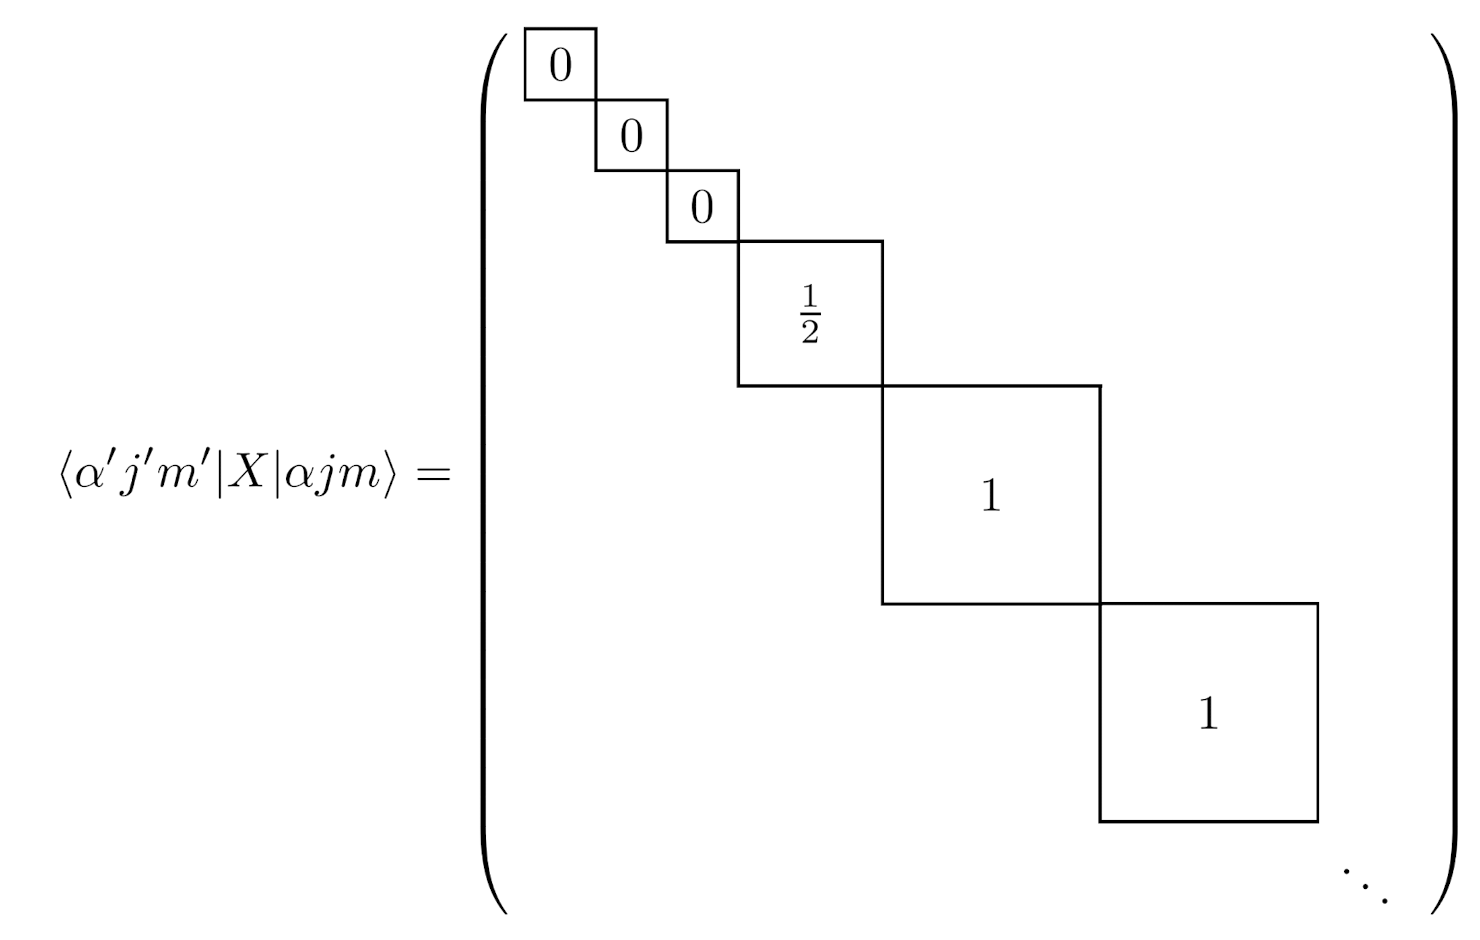
\includegraphics[width = 12cm]{matrix}	
\centering
\vspace{0.1in}
\end{figure}
Le matrici che vanno a sostituirsi al posto dei blocchi lungo la diagonale dipendono dal significato dell'operatore $\hat{X}$, ma la struttura a blocchi rimane la medesima per qualsiasi sua scelta. I blocchi rappresentati nella matrice rappresentano esattamente i sottospazi $\mathcal{E}(k,j)$ di $\mathcal{E}$.

Consideriamo qualche esempio della rappresentazione degli operatori di momento angolare.

\begin{enumerate}
	\item Per $j = 0$ abbiamo che i sottospazi $\mathcal{E}(k,0)$ sono di dimensione $1 \times 1$, di conseguenza le matrici $(J_i)^{(0)}$ sono costituite da un solo numero che \`e zero.
	\item Per $j = 1/2$ abbiamo sottospazi $\mathcal{E}(k,j = 1/2)$ di dimensione $2 \times 2$. Se scegliamo i vettori della base nell'ordine $(m=-1/2,m=1/2)$, usando le regole in (4.10) avremo che 
	\begin{equation*}
		\left(J_z\right)^{(1 / 2)}=\frac{\hbar}{2}\left(\begin{array}{cc}
1 & 0 \\
0 & -1
\end{array}\right)
	\end{equation*} 
	e
	\begin{equation*}
		\left(J_{+}\right)^{(1 / 2)}=\hbar\left(\begin{array}{ll}
0 & 1 \\
0 & 0
\end{array}\right) \quad \quad \left(J_{-}\right)^{(1 / 2)}=\hbar\left(\begin{array}{ll}
0 & 0 \\
1 & 0
\end{array}\right)
	\end{equation*}
	
dato che possiamo definire $J_x$ e $J_y$ nel seguente modo
\begin{equation*}
J_x = \frac{J_+ +J_-}{2} \quad \quad J_y = \frac{J_+ - J_-}{2i}
\end{equation*}
sostituendo le forme matriciali degli operatori di incremento e decremento otteniamo anche quelle di $J_x$ e $J_y$:
\begin{equation*}
	\left(J_x\right)^{(1 / 2)}=\frac{\hbar}{2}\left(\begin{array}{cc}
0 & 1 \\
1 & 0
\end{array}\right) \quad \quad \left(J_y\right)^{(1 / 2)}=\frac{\hbar}{2}\left(\begin{array}{cc}
0 & -i \\
i & 0
\end{array}\right)
\end{equation*}
\newpage
Per l'operatore $\bold{J}^2$ avremo che 
\begin{equation*}
	\left(\mathbf{J}^2\right)^{(1 / 2)}=\frac{3}{4} \hbar^2\left(\begin{array}{ll}
1 & 0 \\
0 & 1
\end{array}\right)
\end{equation*}
\item Per $j = 1 $, e una base nel seguente ordine $(m=1,m=0,m=-1)$, avremo che 
\begin{equation*}
\begin{aligned}
& \left(J_z\right)^{(1)}=\hbar\left(\begin{array}{ccc}
1 & 0 & 0 \\
0 & 0 & 0 \\
0 & 0 & -1
\end{array}\right) \\[0.6cm]
& \left(J_{+}\right)^{(1)}=\hbar\left(\begin{array}{ccc}
0 & \sqrt{2} & 0 \\
0 & 0 & \sqrt{2} \\
0 & 0 & 0
\end{array}\right) \quad \quad \left(J_{-}\right)^{(1)}=\hbar\left(\begin{array}{ccc}
0 & 0 & 0 \\
\sqrt{2} & 0 & 0 \\
0 & \sqrt{2} & 0
\end{array}\right)
\end{aligned}
\end{equation*}
e analogamente al caso precedente 
\begin{equation*}
	\left(J_x\right)^{(1)}=\frac{\hbar}{\sqrt{2}}\left(\begin{array}{ccc}
0 & 1 & 0 \\
1 & 0 & 1 \\
0 & 1 & 0
\end{array}\right) \quad \quad \left(J_y\right)^{(1)}=\frac{\hbar}{\sqrt{2}}\left(\begin{array}{ccc}
0 & -i & 0 \\
i & 0 & -i \\
0 & i & 0
\end{array}\right)
\end{equation*}
e infine 
\begin{equation*}
	\left(\mathbf{J}^2\right)^{(1)}=2 \hbar^2\left(\begin{array}{lll}
1 & 0 & 0 \\
0 & 1 & 0 \\
0 & 0 & 1
\end{array}\right)
\end{equation*}
\end{enumerate}

\section{Spin 1/2 di una particella}

\subsection{Scoperta dello spin: esperimento di Stern-Gerlach}
\begin{wrapfigure}{r}{0.4\textwidth} % 'r' for right; 'l' for left; width of the figure box
    \centering
    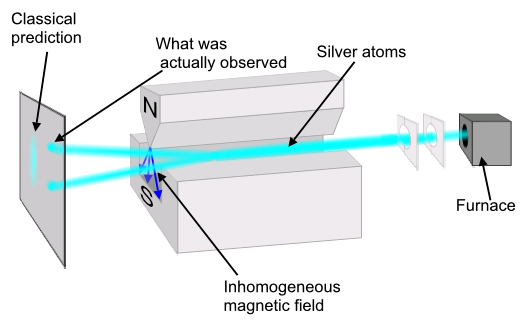
\includegraphics[width=0.38\textwidth]{stern} % Adjust width as needed
    \caption{Apparato sperimentale di Stern-Gerlach.}
\end{wrapfigure}
Una formulazione relativistica della meccani quantistica ci porta a dimostrare che una particella possiede un momento angolare intrinseco che prende il nome di \textit{spin}. La scoperta dei gradi libert\`a dello spin  anticipa lo sviluppo della teoria relativistica della meccanica quantistica di Dirac e viene ottenuta tramite l'esperimento rivoluzionario di Stern-Gerlach (1922). Nel loro esperimento fanno passare un raggio collimato di atomi di argento attraverso una regione in cui \`e presente un campo magnetico disomogeneo prima che queste vadano ad impattare su una superficie fotografica.

Il campo magnetico era diretto perpendicolarmente al fascio, e possedeva un intenso gradiente $\partial_z B_z \neq 0$ in modo tale che il fascio costituito da atomi con momento magnetico venisse deviato lungo l'asse $z$ o $-z$. La forza esercitata sugli atomi di argento \`e proporzionale a $F_z \sim J_z \partial_zB_z$ e la sua posizione proiettata lungo l'asse $z$ sar\`a data dal segno del momento angolare.  Si stima che il fascio di particelle possa comparire in una regione compresa tra $-J_zcost $ e $J_z cost$. Ipotizzando che il momento angolare sulla particella sia dato da  $\hat{J} = \hat{L}$  e sapendo che questo \`e  quantizzato per $j=l = 0,1,....n$ ci aspettiamo di osservare  sul piano fotografico un insieme di $2j+1$ punti lungo l'asse $z$. Sperimentalmente per l'atomo d'argento i punti sono due, il che vuol dire che $2j+1 = 2  \rightarrow j = 1/2$. 
Tale risultato entra in conflitto con l'idea della quantizzazione del momento angolare che avviene per numeri interi e non semi-interi. Il motivo della comparsa di un numero quantico semi-intero \`e dovuta al fatto che in meccanica quantistica \`e presente un momento angolare intrinseco associato alle particelle elementari e composte, che prende il nome di \textit{spin}.
\newline

\noindent Dall'esperimento di Stern-Gerlach, sappiamo che $j = 1/2$ e quindi $m = -1/2,1/2$. Supponiamo di voler creare un fascio polarizzato in cui le particelle possiedono spin solo verso l'alto $\uparrow$,  dall'esperimento di S-G sappiamo gi\`a che i punti osservati rappresentano rispettivamente spin $\uparrow$ e spin $\downarrow$, per selezionare solo lo spin verso l'alto applichiamo un selezionatore chiudendo l'apertura da cui esce il fascio inferiore.

 
\begin{figure}[!ht]
\vspace{0.2in}
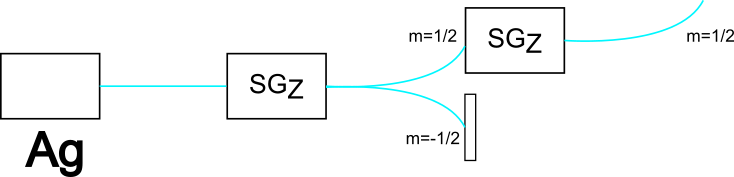
\includegraphics[width = 12cm]{sternGz}	
\centering
\vspace{0.1in}
\end{figure}
Se effettuiamo subito dopo la misura del raggio collimato otteniamo il medesimo risultato, come nella figura soprastante.

Ipotizziamo invece di iniziare ad apporre box dopo l'apparato di Stern-Gerlach con campi magnetici in direzione degli altri assi, per esempio l'asse $x$,  e ch catturi solo gli atomi con spin $\uparrow$ ,quello che osserveremmo sperimentalmente \`e che l'intensit\`a del fascio viene dimezzata, e viene ulteriormente diviso in due parti, rendendo indeterminato il momento angolare $J_x$.

\begin{figure}[!ht]
\vspace{0.2in}
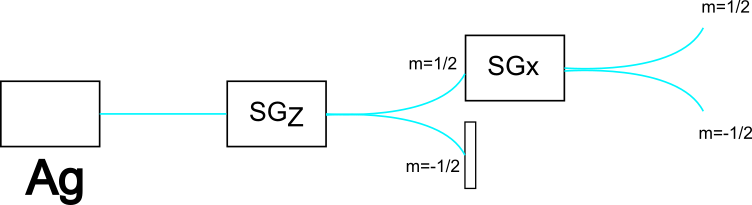
\includegraphics[width = 12cm]{sternGx}	
\centering
\vspace{0.1in}
\end{figure}
Tale risultato \`e dovuto al fatto che i momenti angolari non commutano tra di loro, di conseguenza esiste una regola d'indeterminazione associata ad autostato che risulta essere determinato lungo una direzione, per esempio $z$, ma totalmente indeterminato lungo un altra, come per esempio $x$.

\newpage 

\subsection{Spinori, operatori di spin e matrici di Pauli}

Lo spazio di Hilber del momento angolare per spin 1/2 possiede dimensione due. Per indicare gli autostati si utilizzando diversi tipi di notazione, per esempio da $|l,m \rangle $ si indica $|s,m \rangle$, oppure 
\begin{equation*}
	|1/2,1/2 \rangle = | \uparrow  \rangle = |+ \rangle  \quad \quad |1/2,-1/2 \rangle = |\downarrow \rangle = |-\rangle 
\end{equation*}
 Un stato generico di spin viene indicato come combinazione lineare 
 \begin{equation}
 	\alpha |\uparrow \rangle + \beta |\downarrow \rangle = \left [\begin{array}{c}
 		\alpha \\
 		\beta
 	\end{array}\right ] 
 \end{equation}
con la condizione di normalizzazione $|\alpha|^2 + |\beta|^2 = 1$. Il ket cos\`i definito di dimensione due, prende il nome di \textit{spinore}. Gli operatori che agiscono sugli spinori sono necessariamente matrici $2 \times 2$. Dalla definizione del momento angolare generale definito in precedenza per lo spin valgono tutti i risultati precedentemente ottenuti.
\begin{equation*}
\begin{array}{l}
	\bold{S}^2|s,m \rangle  = \hbar^2s(s+1)|s,m \rangle \\[0.3cm]
	S_z|s,m \rangle = \hbar m|s,m \rangle 
\end{array}
\end{equation*}
nel nostro caso in cui consideriamo $s = 1/2$ abbiamo che le equazioni precedenti assumono l'espressione
\begin{equation}
\begin{array}{l}
	\bold{S}^2|\pm\rangle = \frac{3}{4}\hbar |\pm \rangle \\[0.3cm]
	S_z|\pm \rangle = \pm \frac{\hbar}{2}|\pm \rangle 
\end{array} 
\end{equation}
inoltre valgono le leggi di commutazione $[S_i,S_j] = i\hbar \varepsilon_{ijk}S_k$. Infine possiamo definire gli operatori d'incremento e decremento
\begin{equation}
	\begin{array}{l}
		S_+|s,m \rangle = \hbar \sqrt{s(s+1)-m(m+1)}|s,m \rangle \\[0.3cm]
		S_-|s,m \rangle = \hbar \sqrt{s(s+1)-m(m-1)}|s,m \rangle 
	\end{array}
\end{equation}
Applicando ai ket per $s = 1/2$ avremo che 
\vspace{1cm}
\begin{center}
\begin{tikzpicture}
    \node (A) at (0, 0) {0};
    \node (B) at (3, 0) {$|- \rangle$};
    \draw[->, bend left] (B) to node[below] {$S_-$} (A);
       \node (C) at (6,0) {$| + \rangle $};
    \draw[->, bend left] (C) to node[below] {$S_-$} (B);
    \node (D) at (9,0) {0};
    \draw[->, bend left] (C) to node[above] {$S_+$} (D);
    \draw[->, bend left] (B) to node[above] {$S_+$} (C);
    \draw[->, bend left] (A) to node[above] {$S_+$} (B);
    \draw[->, bend left] (D) to node[below] {$S_-$} (C);
\end{tikzpicture}
\end{center}
Inoltre uno spazio di Hilbert a due stati $\{|-\rangle , |+ \rangle \} $ \`e canonicamente isomorfo a $\mathbb{C}^2$. Di conseguenza possiamo vedere i ket che definiscono una base nello spazio di Hilbert come 
\begin{equation*}
	|+ \rangle = \left [\begin{array}{c}
		1 \\ 0
	\end{array} \right ] \quad \quad  |-\rangle = \left [ \begin{array}{c}
		0\\ 1
	\end{array} \right ]
\end{equation*}
\newpage 


In forma matriciale abbiamo che lo spin lungo l'asse $z$ \`e dato da 
\begin{equation*}
	S_z = \frac{\hbar}{2} \left [ \begin{array}{cc}
		1 & 0 \\
		0 & -1
	\end{array} \right] 
\end{equation*}
definiamo 
\begin{equation*}
	S_+ = \hbar \left [ \begin{array}{cc}
		0 & 1 \\ 
		0 & 0 
	\end{array} \right ] \quad \quad S_- = \hbar  \left [ \begin{array}{cc}
		0 & 0 \\
		1 & 0 
	\end{array} \right ] 
\end{equation*}
dagli  operatori d'incremento e decremento abbiamo che 
\begin{equation*}
	S_x = \frac{S_+ + S_-}{2} = \frac{\hbar }{2} \left [ \begin{array}{cc}
		0 & 1 \\
		1 & 0 
	\end{array} \right ]  \quad \quad S_y = \frac{S_+ - S_-}{2i} = \frac{\hbar }{2} \left [ \begin{array}{cc}
		0 & -i \\
		i & 0
	\end{array}\right ] 
\end{equation*} 
Le matrici legate alle componenti dello spin $\bold{S}$, prendono il nome di \textit{matrici di Pauli} e ci permette di scrivere $\bold{S} = \frac{\hbar}{2} \vec{\sigma}$. Tali matrici sono autoaggiunte e valgono le seguenti propriet\`a:
\begin{enumerate}
	\item $\sigma_i^\dag = \sigma_i$
	\item $\sigma_i^2 =I $
	\item $\sigma_i\sigma_j = - \sigma_j \sigma_i$ \quad \text{per} $i \neq j$ 
	\item $\sigma_i\sigma_j = i \varepsilon_{ijk}\sigma_k$ \quad $i \neq j$
\end{enumerate} 
tali propriet\`a possiamo riassumerle nell'identit\`a 
\begin{equation}
	\sigma_i \sigma_j = I \delta_{ij} + i \varepsilon_{ijk}\sigma_k
\end{equation} 
Se si ha una matrice che rappresenta uno spin condizione necessaria \`e che questi soddisfi le regole di commutazione $[S_i,S_j] = i \hbar \varepsilon_{ijk} \sigma_{k}$. Infine dalle relazioni precedentemente definite, determiniamo
\begin{equation*}
	\bold{S}^2 = \frac{\hbar^2}{4}\vec{\sigma}^2 = \frac{\hbar^2}{4}(\sigma_{x}^2 + \sigma_{y}^2+\sigma_{z}^2) = \frac{3}{4}\hbar^2 I
\end{equation*}

\subsubsection{Esempio}

\begin{wrapfigure}{l}{0.4\textwidth} % 'l' places the figure on the left
    \centering
    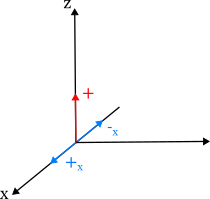
\includegraphics[width=0.3\textwidth]{esempiospin} % Adjust width as needed
\end{wrapfigure}
Consideriamo una configurazione iniziale in cui $| \psi \rangle = |+ \rangle $ e $S_z|+ \rangle  = \frac{\hbar}{2} |+ \rangle $, ovvero lo spin punta in direzione dell'asse $z$. Avremo che effetuata una misura del momento angolare intrinseco della particella lungo l'asse $z$, con probabilit\`a 1 questa assume il valore $\hbar /2$.

Quanto vale la probabilit\`a di una misura lungo $S_x$ ?
\newline

\noindent Sappiamo che 
\begin{equation*}
	S_x = \frac{\hbar}{2} \left [ \begin{array}{cc}
		0 & 1 \\ 
		1 & 0 
	\end{array} \right ]  \quad \text{e} \quad \sigma_1 = \left [ \begin{array}{cc}
		0 & 1 \\ 
		1 & 0 
	\end{array} \right ]
\end{equation*}
Gli autovalori associati alla matrice $\sigma_1$ sono dati dal  polinomio caratteristico $P(\lambda) = (\sigma_1 - \lambda I)$ da cui ricaviamo che $\lambda = \pm 1$. Gli autovettori associati sono dati da 
\begin{equation*}
 (\sigma_1 - \lambda I)_{\lambda = 1} \left [\begin{array}{c}
 	a \\ b
 \end{array} \right ] = \left [\begin{array}{cc}
 	- \lambda & 1 \\
 	1 & - \lambda 
 \end{array} \right ]_{\lambda = 1 } \left [\begin{array}{c}
 	a \\ b
 \end{array} \right ]  = \left [\begin{array}{c}
 	0 \\ 0
 \end{array} \right ]  \iff \left \{ \begin{array}{l}
 	-a + b = 0 \\ 
 	a  - b = 0
 \end{array}\right.
\end{equation*}
e quindi per $\lambda = 1$ l'autovettore associato \`e dato dato da $[a \; a]^T$. Analogamente per $\lambda = -1$ avremo $[a \; -a]^{T}$. Preso $a = 1$, riscriviamo gli autovettori normalizzati
\begin{equation*}
	| + \rangle_{x} = \frac{1}{\sqrt{2}} \left [\begin{array}{l}
		1 \\
1	\end{array}\right ]  \quad \quad |-\rangle_{x} = \frac{1}{\sqrt{2}} \left [\begin{array}{c}
		1 \\ -1	\end{array}\right ] 
\end{equation*}
Dunque la probabilit\`a che 
\begin{align*}
	P(S_x = \hbar/2) = | \langle +_x |\psi \rangle|^2 = \left | [1/\sqrt{2}, 1/\sqrt{2}] \cdot \left [\begin{array}{c}
		1 \\ 0
	\end{array} \right ] \right |^2 = 1/2 \\[0.5cm]
	P(S_x = -\hbar/2) = | \langle -_x |\psi \rangle|^2 = \left | [1/\sqrt{2}, -1/\sqrt{2}] \cdot \left [\begin{array}{c}
		0\\ 1
	\end{array} \right ] \right | ^2 = 1/2
\end{align*}
Fissato lo spin lungo l'asse $z$ e fatta una misura lungo una direzione ortogonale, si ha indeterminazione nel risultato. Che cosa succede per una direzione generica ?

\subsection{Relazione tra uno spinore e la direzione dello spin}
\begin{wrapfigure}{r}{0.4\textwidth} % 'r' for right; 'l' for left; width of the figure box
    \centering
    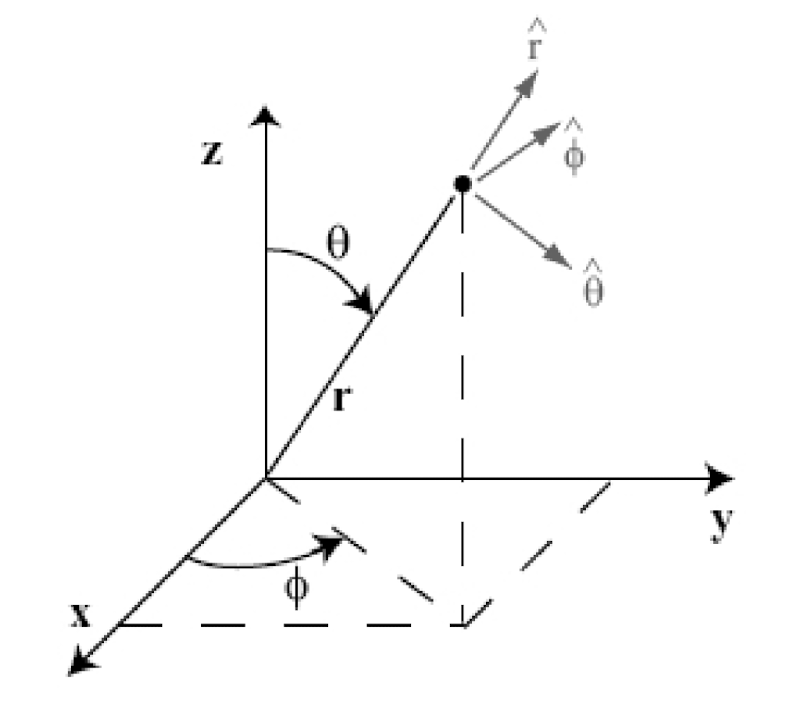
\includegraphics[width=0.38\textwidth]{spinrotation} % Adjust width as needed
\end{wrapfigure}

Per uno stato generico $\alpha |+ \rangle + \beta |- \rangle $, le componenti $\alpha $ e $\beta$ come si relazione al modo in cui lo spin della particella \`e orientato? per rispondere alla domanda, assumiamo che lo spin punti lungo il vettore unitario
\begin{equation*}
	\hat{\bold{n}} = (\sin \theta \cos \phi , \sin \theta \sin \phi, \cos \theta)
\end{equation*}
per esempio nella direzione data da $(\theta, \phi)$. In sostanza lo spin \`e un autostato dell'operatore $\vec{\sigma } \cdot \hat{\bold{n}} = \bold{S} \cdot \hat{\bold{n}}$. In modo esplicito avremo che 

\begin{align*}
	\vec{\sigma} \cdot \hat{\bold{n}} = & \sin\theta \cos \phi \left [ \begin{array}{cc} 1 & 0 \\ 0 & 1\end{array}\right ] + \sin \theta \sin \phi \left [ \begin{array}{cc} 0 & -i \\ i & 0\end{array}\right ] + \cos \theta \left [ \begin{array}{cc} 1 & 0 \\ 0 & -1\end{array}\right ] = \\[0.5cm]
	= &\left [ \begin{array}{cc}
		\cos \theta &  \sin \theta e^{i\phi} \\[0.5cm]
		\sin \theta e^{-i\phi} & - \cos \theta 
	\end{array} \right ] 
\end{align*}
inoltre vale la propriet\`a in cui $(\vec{\sigma} \cdot \hat{\bold{n}})^2 = I$. 
\newpage 

Gli autovalori della matrice sono dati da $\pm 1$ e gli autovettori associati:

\begin{equation*}
	|+ \rangle_{\bold{n}} = \left [ \begin{array}{c}
		\cos \frac{\theta}{2} \; e^{-i\phi/2}\\
		\sin \frac{\theta}{2} \; e^{i\phi/2}
	\end{array}\right] \quad \quad |- \rangle_{\bold{n}} = \left [\begin{array}{c}
		- \sin \frac{\theta}{2} \; e^{-i\phi/2} \\
		\cos \frac{\theta}{2} \; e^{i \phi/2}
	\end{array} \right]
\end{equation*}
Possiamo riscrivere gli autovettori rispetto alla base di Hilbert formati dagli elementi $|+ \rangle $ e $|- \rangle$ che sono autostati di $S_z$, nel seguente modo
\begin{align*}
	&|+ \rangle_{\bold{n}} = \cos \frac{\theta}{2} \; e^{-i\phi/2} |+ \rangle + \sin \frac{\theta}{2} \; e^{i\phi/2} |-\rangle \\[0.5cm]
	&|- \rangle_{\bold{n}} =   - \sin \frac{\theta}{2} \; e^{-i\phi/2} |+ \rangle + \cos \frac{\theta}{2} \; e^{i \phi/2}|- \rangle 
\end{align*}
Gli operatori $S_x,S_y$ e $S_n$ hanno gli stessi autovalori $\pm \hbar /2$ di $S_z$. Tale risultato \`e abbastanza intuitivo in quando basta ruotare l'apparato di Stern-Gerlach, ponendo il campo magnetico parallelo a $Ox$ o $Oy$ o anche $\bold{n}$. Dunque se vogliamo calcolare la probabilit\`a per una generica direzione $\bold{n}$ avremo che 
\begin{align*}
	& P(\bold{S} \cdot \bold{n} = \hbar /2 ) = |\langle +_{\bold{n}} | \psi \rangle |^2 = \cos^2 \frac{\theta }{2} \\[0.5cm]
	& P(\bold{S} \cdot \bold{n} = - \hbar /2) = |\langle -_{\bold{n}} | \psi \rangle |^2= \sin^2 \frac{\theta }{2} 
\end{align*}

\subsection{Precessione dello spin in un campo magnetico: Precessore di Larmor}

\begin{wrapfigure}{r}{0.4\textwidth} % 'l' places the figure on the left
    \centering
    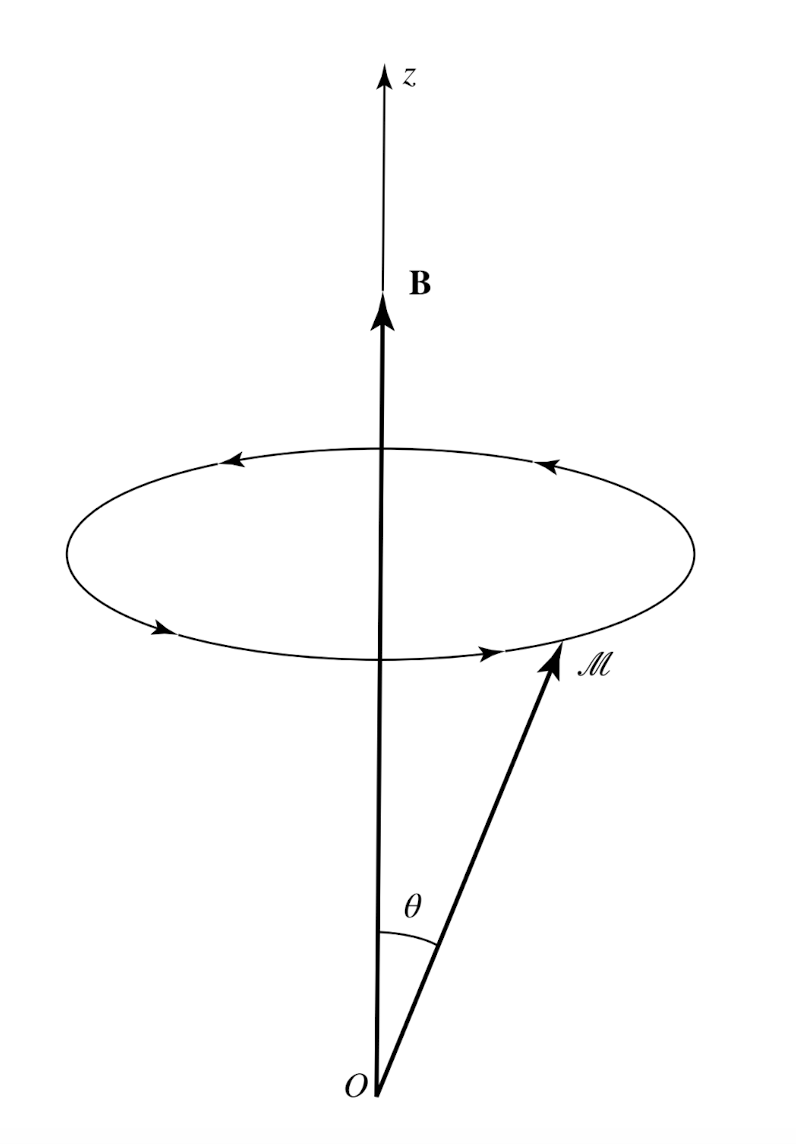
\includegraphics[width=0.3\textwidth]{magnetic} % Adjust width as needed
\end{wrapfigure}

Consideriamo un oggetto magnetizzato classicamente che ruota attorno al suo centro di massa, con momento angolare $\bold{L}$ e con momento magnetico $\boldsymbol{\mu} = \gamma \bold{L}$ parallelo.
 Dove il termine $\gamma$ \`e la costante di rapporto giromagnetico. Ipotizziamo che il campo magnetico $\bold{B}$ abbia direzione lungo l'asse $z$. Il momento della forza esercitato sar\`a dato da 
 \begin{equation*}
 	\frac{d \bold{L}}{dt} = \bold{T} = \boldsymbol{\mu} \times \bold{B} = \gamma \bold{L} \times \bold{B} 
 \end{equation*}
 
Risolvendo l'equazione si dimostra che il momento angolare $\bold{L}$  precede attorno alla direzione in cui punta il campo magnetico con una frequenza $\omega_0 = - \gamma \bold{B}$, che prende il nome di \textit{frequenza di Larmor}. Di seguito dimostriamo che i medesimi risultati si hanno nello studio della meccanica quantistica dello spin di un elettrone in un campo magnetico.
\newline

\noindent Un elettrone ha un momento di dipolo magnetico $\boldsymbol{\mu} = \gamma \bold{S}$ dove il rapporto giromagnetico \`e dato da $\gamma = g \frac{-e}{2m_e}$. La Hamiltoniana che descrive l'interazione con il momento di dipolo dell'elettrone e il campo magnetico \`e data da
\begin{equation*}
	\hat{H} =- \boldsymbol{\mu} \cdot \bold{B} = - \gamma \bold{S} \cdot \bold{B}
\end{equation*} 
\newpage

Introduciamo un nuovo operatore che definisce la rotazione dello spin. In generale, l'operatore di rotazione per una rotazione di un angolo $\theta$ rispetto ad un asse che ha direzione lungo il vettore unitario $\bold{\hat{n}}$ \`e dato da $e^{i \theta \bold{\hat{n}} \cdot \bold{J}/ \hbar}$ dove $\bold{J}$ \`e l'operatore di momento angolare generale. Posto $\bold{J} = \bold{S} = \frac{1}{2}\hbar \boldsymbol{\sigma}$ l'operatore di rotazione assume la forma 
\begin{equation*}
	e^{(i \theta /2)(\bold{\hat{n}} \cdot \boldsymbol{\sigma})} = I \cos(\theta/2) + i \bold{\hat{n}} \cdot \boldsymbol{\sigma} \sin(\theta/2) 
\end{equation*}  
L'operatore di rotazione \`e esprimibile come una matrice $2 \times 2$ nello spazio degli stati. Tale matrice \`e unitaria. Inoltre notare che per una rotazione attorno all'asse $z$, si ha che $\bold{\hat{n}} = (0,0,1)$, in questo caso \`e pi\`u naturale sostituire $\theta$ con $\phi$, e l'operatore di rotazione assume la forma matriciale
\begin{equation*}
	e^{i(\theta / 2)(\mathbf{n} \cdot \boldsymbol{\sigma})}=\left(\begin{array}{cc}
e^{-i \phi / 2} & 0 \\
0 & e^{i \phi / 2}
\end{array}\right)
\end{equation*}
Tornando alla discussione dello spin avremo che dato uno stato iniziale $| \psi (0) \rangle $ per un tempo $t = 0$ in cui si trova il sistema, il suo evoluto temporale sar\`a dato dall'applicazione dell'operatore di evoluzione temporale allo stato di partenza
\begin{equation*}
	|\psi(t) \rangle = \hat{U}(t)|\psi(0) \rangle 
\end{equation*}
dove 
\begin{equation*}
	\hat{U}(t) = e^{-i\hat{H}t/\hbar} = e^{i \gamma \boldsymbol{\sigma} \cdot \bold{B}t/2}
\end{equation*}
ma questo non \`e altro che l'operatore di rotazione definito in precedenza, rispetto ad angolo $- \gamma Bt$ rispetto alla direzione di $\bold{B}$. 

Se consideriamo per esempio un orientazione iniziale arbitraria dello spin \`e data da
\begin{equation*}
	|+ \rangle_{\bold{\hat{n}}} = \binom{e^{-i \phi / 2} \cos (\theta / 2)}{e^{i \phi / 2} \sin (\theta / 2)}
\end{equation*}
l'operatore di evoluzione temporale lungo la direzione $z$ \`e assume l'espressione
\begin{equation*}
	U(t)=e^{i \gamma \boldsymbol{\sigma} \cdot \mathbf{B} t / 2}=\left(\begin{array}{cc}
e^{-i \omega_0 t / 2} & 0 \\
0 & e^{i \omega_0 t / 2}
\end{array}\right)
\end{equation*}
e dunque lo stato ad un tempo $t$ si esprime nel seguente modo
\begin{equation*}
	|+ (t) \rangle_{\bold{\hat{n}}} = \binom{e^{-i\left(\phi+\omega_0 t\right) / 2} \cos (\theta / 2)}{e^{i\left(\phi+\omega_0 t\right) / 2} \sin (\theta / 2)}
\end{equation*}
L'angolo $\theta$ tra lo spin e il campo resta costante mentre l'angolo azimutale attorno al campo aumenta di $\phi = \phi_0 + \omega_0t$, come nel caso classico.

\newpage 
\section{Esempi ed Esercizi per lo spin di una particella}

\subsection{Esercizio 1}

Si consideri al tempo $t = 0 $ una particella di spin $1/2$ nello stato iniziale  $|\psi(0) \rangle  = |+ \rangle $ orientata lungo l'asse $z$. Determinare:
\begin{enumerate}
	\item La probabilit\`a per $S_x$  al tempo $t=0$
	\item In presenza di campo magnetico $\bold{B} = B_0\bold{e}_y$, la probabilit\`a al tempo $t$ per $S_x,S_y$ e $S_z$  
\end{enumerate}

\begin{proof}
	
	In forma vettoriale lo stato di partenza coicide con il vettore
	\begin{equation*}
		|+ \rangle = \left [ \begin{array}{c}
			1 \\ 0 
		\end{array} \right ] 
	\end{equation*}
1) Per calcolare la probabilit\`a lungo l'asse $x$, dobbiamo decomporre il vettore di stato iniziale rispetto agli autovettori normalizzati della matrice $\sigma_1$ di Pauli
\begin{equation*}
	|+ \rangle_x = \frac{1}{\sqrt{2}} \left [ \begin{array}{c}
		1 \\ 1
	\end{array} \right ] \quad \quad |- \rangle_x = \frac{1}{\sqrt{2}} \left [ \begin{array}{c}
		1 \\ -1
	\end{array} \right ]
\end{equation*}
e dunque 
\begin{equation*}
	|+ \rangle  = \frac{|+ \rangle_x + |- \rangle_x}{\sqrt{2}}
\end{equation*}
e quindi
\begin{align*}
	P\left (S_x = \frac{\hbar}{2} \right ) = |\langle + |_x+\rangle|^2 = \frac{1}{2}\\[0.3cm]
	P\left (S_x = -\frac{\hbar}{2} \right ) = |\langle - |_x+\rangle|^2 = \frac{1}{2}\\[0.3cm] 
\end{align*}
2) La descrizione dinamica di una particella con momento angolare all'interno di un campo magnetico \`e data dalla Hamiltoniana
\begin{equation*}
	\hat{H} = - \boldsymbol{\mu} \cdot \bold{B} = - \gamma \bold{S} \cdot \bold{B} = -\gamma B_0S_y 
\end{equation*}
Scriviamo lo stato iniziale rispetto agli autovettori normalizzati della matrice di Pauli $\sigma_2$ associata all'operatore di spin $S_y$, che sono dati da 
\begin{equation*}
	|+ \rangle_y = \frac{1}{\sqrt{2}} \left [ \begin{array}{c}
		1 \\ i
	\end{array} \right ] \quad \quad |- \rangle_y = \frac{1}{\sqrt{2}} \left [ \begin{array}{c}
		1 \\ -i
	\end{array} \right ]
\end{equation*}
e quindi 
\newpage 

\begin{equation*}
	|+ \rangle = \frac{|+ \rangle_y + | - \rangle_y}{\sqrt{2}}
\end{equation*}
Troviamo l'evoluto temporale di uno stato, in questo caso, applicando l'operatore di rotazione $\hat{U}$ allo stato di partenza
\begin{align*}
	|\psi(t) \rangle = &  \frac{1}{\sqrt{2}}e^{-i/\hbar (-\gamma B_0 \hbar/2 )t}|+\rangle_y + \frac{1}{\sqrt{2}} e^{- i / \hbar (\gamma B_0 \hbar / 2)t}|- \rangle_- = \\[0.3cm]
	= &  \frac{1}{\sqrt{2}}e^{i (\gamma B_0/2 )t}|+\rangle_y + \frac{1}{\sqrt{2}} e^{- i (\gamma B_0 / 2)t}|- \rangle_-  =  \left [\begin{array}{c}
		\cos(\frac{\gamma B_0t}{2}) \\[0.2cm]
		-\sin (\frac{\gamma B_0t}{2})
	\end{array}\right]
\end{align*}
Le probabilit\`a relative agli operatori richiesti dall'esercizio saranno date da 
\begin{align*}
	&P \left (S_z  = \frac{\hbar}{2} \right ) = | \langle + |_z  \psi(t) \rangle |^2 = \cos^2 \left (\frac{\gamma B_0 t}{2} \right ) \\[0.5cm]
	&P \left (S_z  = -\frac{\hbar}{2} \right ) = | \langle - |_z  \psi(t) \rangle |^2 = \sin^2 \left (\frac{\gamma B_0 t}{2} \right ) \\[0.5cm] 
	&P \left (S_x = \frac{\hbar}{2} \right ) = | \langle + |_x  \psi(t) \rangle |^2 =  \frac{1}{2} \left | \cos \left (\frac{\gamma B_0 t}{2} \right ) - \sin \left (\frac{\gamma B_0 t}{2} \right )  \right |^2 \\[0.5cm]
	&P \left (S_x = -\frac{\hbar}{2} \right ) = | \langle - |_x  \psi(t) \rangle |^2 =  \frac{1}{2} \left | \cos \left (\frac{\gamma B_0 t}{2} \right ) + \sin \left (\frac{\gamma B_0 t}{2} \right )  \right |^2 \\[0.5cm]
	&P \left (S_y = \frac{\hbar}{2} \right ) = | \langle + |_y  \psi(t) \rangle |^2 =  \frac{1}{2} \left | \cos \left (\frac{\gamma B_0 t}{2} \right ) + i \sin \left (\frac{\gamma B_0 t}{2} \right )  \right |^2 = |e^{i \gamma B_0/2}|^2 = \frac{1}{2} \\[0.5cm]
	&P \left (S_y = -\frac{\hbar}{2} \right ) = | \langle - |_y  \psi(t) \rangle |^2 =  \frac{1}{2} \left | \cos \left (\frac{\gamma B_0 t}{2} \right ) - i \sin \left (\frac{\gamma B_0 t}{2} \right )  \right |^2 = |e^{-i \gamma B_0/2}|^2 = \frac{1}{2} 
\end{align*}
Metodo 2) 
\newline
Utilizziamo la definizione di operatore di rotazione 
\begin{equation*}
	e^{i(\theta/2)\bold{S} \cdot \bold{n}} = I \cos \left (\frac{\theta}{2} \right ) + i \;\bold{n} \cdot \boldsymbol{\sigma} \sin \left (\frac{\theta}{2} \right)
\end{equation*}
consideriamo come direzione quella lungo l'asse $y$, data dal versore $\bold{n} = [0,1,0]$
e dunque avremo che l'operatore assume la forma matriciale
\begin{equation*}
	e^{i(\theta/2)\bold{S} \cdot \bold{n}} = \left [\begin{array}{cc}
		\cos(\theta/2) & \sin(\theta/2) \\
		- \sin(\theta/2) & \cos(\theta/2)
	\end{array} \right ]
\end{equation*}
che coincide con l'operatore di evoluzione temporale $U = e^{-iHt/\hbar}$ per $\theta = \gamma B_y t$. Applicandolo allo stato di partenza otteniamo i risultati del primo metodo.

\end{proof}
\newpage 

Abbiamo visto che per $t = 0$ si ha una probabilit\`a di 1/2 e 1/2 lungo gli assi ortogonali alla direzione dello stato.  La Hamiltoniana essendo dipendente da $S_y$ commuta con $S_y$ di conseguenza avremo che $S_y$ \`e una costante del moto e la probbailit\`a non pu\`o dipendere dal tempo.

\subsection{Esercizio 2}

Definire lo spin lungo il versore 
\begin{equation*}
	\bold{\hat{n}} = \frac{1}{\sqrt{3}} \left [ \begin{array}{c}
		1 \\ 1 \\ 1
	\end{array}\right ]
\end{equation*}
Determinare la probabilit\`a che misurando lo spin nella direzione $z$, si abbia $S_z = \hbar /2 $. 

\begin{proof}
	Dalla teoria sappiamo che  $\bold{S} \cdot \bold{n} = \frac{\hbar}{2} \boldsymbol{\sigma} \cdot \bold{n}$ per $\bold{n} = (\cos \phi \sin \theta, \sin \phi \sin \theta, \cos \theta )$. Gli stati sono descritti dai ket 
	\begin{equation*}
		|+ \rangle_{\bold{n}} = \left [ \begin{array}{c}
		\cos \frac{\theta}{2} \; e^{-i\phi/2}\\
		\sin \frac{\theta}{2} \; e^{i\phi/2}
	\end{array}\right] \quad \quad |- \rangle_{\bold{n}} = \left [\begin{array}{c}
		- \sin \frac{\theta}{2} \; e^{-i\phi/2} \\
		\cos \frac{\theta}{2} \; e^{i \phi/2}
	\end{array} \right]
	\end{equation*}
e dunque la probabilit\`a lungo $z$ di misurare $S_z = \hbar /2$ \`e data da
\begin{equation*}
	P(S_z = \hbar /2) = |\langle + | \psi \rangle |^2 = \cos^2 \left (\frac{\theta}{2} \right )
\end{equation*}	
dove dalla relazione del versore dello spin sappiamo che $\cos \theta = \frac{1}{\sqrt{3}}$. Usando la formula di duplicazione 
\begin{equation*}
	P(S_z = \hbar/2) = \frac{\cos\theta + 1}{2} = \frac{1 + 1/ \sqrt{3}}{2}
\end{equation*}
\end{proof}

\subsection{Esercizio 3}
Data la Hamiltoniana $H = - \boldsymbol{\omega} \cdot \bold{S}$ per una particella di spin 1/2 che si trova nella configurazione iniziale $|\psi(0) \rangle = |+ \rangle $ al tempo $t = 0$, calcolare la probabilit\`a che $S_z = \hbar /2$ al tempo $t$.
\begin{proof}
	Metodo 1)
	\newline
	Consideriamo $\boldsymbol{\omega}$ come un cambio magnetico con un orientazione generica $\boldsymbol{\omega} = |\omega|\bold{n}$, per $\bold{n}$ versore. Riscriviamo la Hamiltoniana rispetto ad un verose generico
	\begin{equation*}
		\hat{H} = - |\omega| \bold{n} \cdot \bold{S} = - |\omega| \; \frac{\hbar}{2} \; \boldsymbol{\sigma} \cdot \bold{n}
	\end{equation*}
Gli autostati associati sono quelli definiti in precedenza $|+ \rangle_{\bold{n}}$ e $|- \rangle_{\bold{n}}$. Rappresentiamo lo stato iniziale rispetto alla base di autovettori per una direzione generica
\begin{equation*}
	|+ \rangle = \langle + |_{\bold{n}} + \rangle \;|+ \rangle_{\bold{n}} + \langle -|_{\bold{n}}- \rangle \;|-\rangle_{\bold{n}}
\end{equation*}
\newpage

dove 
\begin{equation*}
	\langle + |_{\bold{n}} + \rangle = \cos (\theta /2)e^{i \phi /2} \quad \quad \langle -|_{\bold{n}}- \rangle = - \sin(\theta /2)e^{i \phi /2}
\end{equation*}
e quindi lo stato di partenza rispetto agli autovettori generali assume la forma 
\begin{equation*}
	|+ \rangle = \cos(\theta/2) \; |+ \rangle_{\bold{n}} + \sin(\theta/2) \; |- \rangle_{\bold{n}}
\end{equation*}
applicando l'operatore di evoluzione temporale, considerando gli autovalori $\pm \hbar/2$, avremo che 
\begin{equation*}
	|\psi(t) \rangle = \cos(\theta /2) e^{i \phi/2}e^{i|\omega|t/2}\; |+\rangle_{\bold{n}} - \sin(\theta /2) e^{i \phi /2 }e^{-i|\omega|t/2}\;|- \rangle_{\bold{n}}
\end{equation*}
Infinire possiamo calcolare la probabilti\`a che $S_z = \hbar/2$ come rischiesto dal problema calcolando il prodotto scalare 
\begin{align*}
	P(S_z = \hbar /2) = & | \langle + | \psi(t)\rangle |^2 = \left | \cos^2 \left ( \frac{\theta}{2}\right ) e^{i \phi/2}e^{i|\omega|t/2}  + \sin^2 \left( \frac{\theta}{2}\right) e^{i \phi/2}e^{-i|\omega|t/2}\right|^2 = \\[0.5cm]
	= & \left | \cos \left (\frac{|\omega|t}{2} \right ) + i \sin \left( \frac{|\omega|t}{2} \right )\cos\theta\right |^2
\end{align*}
Metodo 2) 
\newline
Esprimiamo lo stato ad un tempo $t$ nel seguente modo
\begin{equation*}
	|\psi(t) \rangle = e^{-iHt/\hbar}|\psi(0) \rangle  = e^{-i/\hbar (|\omega| [\bold{S} \cdot \boldsymbol{\sigma}]t)}|\psi(0) \rangle = e^{-i \frac{|\omega|t}{2}(\boldsymbol{\sigma} \cdot \bold{n})}|\psi(0) \rangle = e^{-i \alpha (\boldsymbol{\sigma} \cdot \bold{n})}|\psi(0) \rangle
\end{equation*}
Sapppiamo che un termine $e^{i \alpha (\boldsymbol{\sigma} \cdot \bold{n})}$ prende il nome di matrice esponenziale e pu\`o essere espressa come serie di potenze 
\begin{equation*}
	e^{X} = \sum_{k=0}^{\infty} \frac{1}{k!} X^k
\end{equation*}
posto $X = -i\alpha(\boldsymbol{\sigma} \cdot \bold{n})$ avremo che 
\begin{equation*}
	e^{-i \alpha (\boldsymbol{\sigma} \cdot \bold{n})} =  I-i \alpha (\boldsymbol{\sigma} \cdot \bold{n}) + \frac{1}{2} (-i)^2 \alpha^2 \underbrace{(\boldsymbol{\sigma} \cdot \bold{n})^2}_{=I} + \frac{1}{3!}(-i)^3 \alpha^3 (\boldsymbol{\sigma} \cdot \bold{n})^3 + ...
\end{equation*}
dunque possiamo dividere l'espansione in termini pari e termini dispari, effettuando gli opportuni raccoglimenti avremo che 
\begin{align*}
	e^{-i \alpha (\boldsymbol{\sigma} \cdot \bold{n})} = & \; I \left (1-\frac{\alpha^2}{2} + ... \right  ) - i(\boldsymbol{\sigma} \cdot \bold{n}) \left ( \alpha - \frac{\alpha}{3!} + ...\right ) =  \\[0.5cm]
	 = & \; I \; \sum_{k=0}^{\infty} \frac{(-1)^{2n}}{2n!}\alpha^{2n}  -i(\boldsymbol{\sigma} \cdot \bold{n}) \; \sum_{k=0}^{\infty} \frac{(-1)^{2n+1}}{(2n+1)!} \alpha^{2n+1} = \\[0.5cm]
	 = & \; I\cos(\alpha) - i(\boldsymbol{\sigma} \cdot \bold{n}) \sin(\alpha)
\end{align*}
Definito l'operatore di evoluzione temporale nella sua forma matriciale $2 \times 2$ possiamo procede al
\newpage
calcolo della probabilit\`a, ottenendo lo stesso risultato del metodo 1.

\end{proof}

\subsection{Esercizio 4: Particelle con spin 1}

Consideriamo una particella di spin 1 all'interno di un campo magnetico, la cui evoluzione dinamica \`e descritta dalla Hamiltoniana
\begin{equation*}
	H = \gamma \bold{S} \cdot \bold{B} =\gamma BS_x
\end{equation*}
La particella al tempo $t = 0$ si trova nello stato $|1,1  \rangle $. Calcolare la probabilit\`a che al tempo $t$ sia nello stato $|1,-1 \rangle $.
\begin{proof}
	Un tipo di particelle fondamentali che possiedono spin 1 \`e dato dai \textit{fotoni}. I valori possibili del momento angolare sono dati da $S_z = - \hbar ,0, \hbar $ per $m = -1,0,1$. In particolare per una particella di spin 1 individuiamo uno spazio di Hilbert di dimensione tre per l'operatore $S_z$ i cui elementi della base sono i suoi autovettori
	\begin{equation*}
		|11 \rangle = \left [ \begin{array}{c}
		1 \\ 0 \\ 0 
 		\end{array} \right ] \quad \quad |1,0 \rangle = 	\left [ \begin{array}{c}
		0 \\1 \\ 0 
 		\end{array} \right ] \quad \quad |1,-1 \rangle = \left [ \begin{array}{c}
		0 \\ 0 \\ 1 
 		\end{array} \right ]
	\end{equation*}
In forma matriciale l'operatore $S_Z$ \`e rappresentato da una matrice di dimensione $3 \times 3$,
\begin{equation*}
	S_z = \hbar \left [  \begin{array}{ccc} 1 & 0 & 0 \\
	0 & 0 & 0 \\
	0 & 0 & -1
	\end{array}\right ] 
\end{equation*}
e gli operatori d'incremento e riduzione sono analogamente rappresentati nel seguente modo
\begin{equation*}
	S_+ = \hbar \sqrt{2} \left [ \begin{array}{ccc}
		0 & 1 & 0 \\
		0 & 0 & 1 \\
		0 & 0 & 0 
	\end{array}\right ] \quad \quad S_- = \hbar \sqrt{2} \left [ \begin{array}{ccc}
		0 & 0 & 0 \\
		1 & 0 & 0 \\
		0 & 1 & 0 
	\end{array}\right ]
\end{equation*}
infine 
\begin{equation*}
	S_x = \frac{S_+ + S_-}{2} = \frac{\hbar}{\sqrt{2}} \left [ \begin{array}{ccc}
		0 & 1 & 0 \\
		1 & 0 & 1 \\
		0 & 1 & 0 
	\end{array}\right ] \quad \quad S_y = \frac{S_+ - S_-}{2i} = \frac{\hbar}{\sqrt{2}}\left [ \begin{array}{ccc}
		0 & -i & 0 \\
		i & 0 & -i \\
		0 & i & 0 
	\end{array}\right ]
\end{equation*}
Per le ragioni discusse nei paragrafi precedenti di questo capitolo gli autovalori associati agli operatori $S_x$ e $S_y$ sono i medesimi di quelli di $S_z$, e gli autovettori associati sono dati da 
\begin{align*}
		|10 \rangle_x =  \frac{1}{\sqrt{2}}\left [ \begin{array}{c}
		1 \\ 0 \\ -1 
 		\end{array} \right ] \quad \quad |1,1 \rangle_x = \frac{1}{2}	\left [ \begin{array}{c}
		1 \\\sqrt{2} \\ 1 
 		\end{array} \right ] \quad \quad |1,-1 \rangle_x =  \frac{1}{2} \left [ \begin{array}{c}
		1 \\ - \sqrt{2} \\ 1 
 		\end{array} \right ]
\end{align*}
\newpage
\begin{equation*}
		|10 \rangle_y =  \frac{1}{\sqrt{2}}\left [ \begin{array}{c}
		1 \\ 0 \\ 1 
 		\end{array} \right ] \quad \quad |1,1 \rangle_y = \frac{1}{2}	\left [ \begin{array}{c}
		1 \\ i\sqrt{2} \\ -1 
 		\end{array} \right ] \quad \quad |1,-1 \rangle_y =  \frac{1}{2} \left [ \begin{array}{c}
		1 \\ - i\sqrt{2} \\ -1 
 		\end{array} \right ]
\end{equation*}
Per rispondere alla domanda posta dall'esercizio, risicriviamo lo stato di partenza della particella rispetto alla base di autovettori di $S_x$
\begin{align*}
	|11\rangle = & \; \langle 11|_{x}11 \rangle \; |11\rangle_{x} + \langle 10|_x11\rangle \; |10\rangle_x + \langle 1 -1|_x11 \rangle  \; |1-1 \rangle_x  = \\[0.5cm] 
	= & \; \frac{1}{2} |11 \rangle_x \; + \; \frac{1}{\sqrt{2}} |10 \rangle_x \; + \; \frac{1}{2} |1-1 \rangle_x
\end{align*}
Gli autovalori associati all'operatore H sono dati da 
\begin{equation*}
	|11 \rangle_x \to \gamma B\hbar \quad \quad |10 \rangle_x \to 0 \quad \quad |1-1 \rangle_x \to -\gamma B\hbar 
\end{equation*}
e dunque lo stato al tempo $t$ \`e dato da 
\begin{equation*}
	|\psi(t) \rangle = \frac{e^{-i\gamma B t}}{2} |11 \rangle_x + \frac{e^{i\gamma Bt}}{2}|1-1\rangle_x + \frac{1}{2} |10 \rangle_x
\end{equation*}
e la probabilit\`a che al tempo t $S_z = -\hbar $ \`e data da 
\begin{equation*}
	P(S_z = - \hbar) = |\langle 1-1 | \psi(t) \rangle |^2 = \left |  \frac{e^{-i\gamma Bt} + e^{i \gamma Bt}}{4} - \frac{1}{2}\right |^2 = \left |  \frac{\cos(\gamma B t) -1}{2}\right |^2 = \frac{1}{2}\sin^4(\gamma B t) 
\end{equation*}

\end{proof}

\subsection{Esercizio 5}

Consideriamo un sistema che si trova nella configurazione iniziale 
\begin{equation*}
	|\psi(0) \rangle = \frac{f(r)}{\sqrt{8\pi}} \left (1+ \frac{x +iy +z}{r}\right)
\end{equation*}
dove per $f(r)$ si ha che $\int_{0}^{\infty} r^2 |f(r)|^2 = 1$ e la cui evoluzione dinamica \`e descritta dalla Hamiltoniana 
\begin{equation*}
	H = gL_z
\end{equation*}
Qaul \`e la probabilit\`a per $L_2,L_x,L_y$ e $L_z$ al generico tempo $t$ ?

\begin{proof}
Per i momenti angolari ricordiamo che la funzione d'onda soluzione delle equazioni \`e data da 
\begin{equation*}
	|\psi(r) \rangle = f(r)Y_{m}^l(\theta,\phi)
\end{equation*}	
richiedere che la funzione d'onda sia normalizzata equivale a chiedere che
\begin{equation*}
	1 = \int d\bold{x}|\psi|^2 = \int_{0}^{\infty}dr \; r^2|f(r)|^2 \int_{\Omega} d\Omega \; |Y_{m}^l|^2 
\end{equation*}
\newpage

dato che ipotesi iniziale il termine radiale della funzione d'onda \`e gi\`a normalizzato, il problema richiede un analisi solo rispetto alla componente angolare. Procediamo con il riscrivere lo stato iniziale rispetto alle armoniche sferiche
\begin{equation*}
	Y_{00} = \frac{1}{\sqrt{4\pi}} \quad \quad  Y_{11} = \sqrt{\frac{3}{4 \pi}} \cos(\theta) = \sqrt{\frac{3}{4 \pi}} \frac{z}{r} \quad \quad Y_{1 \pm 1} = \pm \sqrt{\frac{3}{8 \pi}} \sin \theta e^{\pm i \phi} = \pm \sqrt{\frac{3}{8\pi}} \frac{x \pm i y}{r}
\end{equation*}
e quindi 
\begin{equation*}
	|\psi(0) \rangle = \frac{1}{\sqrt{2}}Y_{00} - \frac{1}{\sqrt{3}}Y_{11} + \frac{1}{\sqrt{6}}Y_{10}
\end{equation*}
opportunamente normalizzato.

Ricordiamo che l'autovalore associato a $L_z$ \`e dato da $\hbar m$, dunque al tempo $t$ l'evoluto temporale \`e dato da 
\begin{equation*}
	|\psi(t) \rangle = \frac{1}{\sqrt{2}}Y_{00} - \frac{1}{\sqrt{3}}Y_{11}e^{-igt} + \frac{1}{\sqrt{6}}Y_{10}
\end{equation*}
Le probabilit\`a associate agli operatori $\bold{L}^2$ e $\bold{L_z}$ per $m = 0,1$ e $l = 0,1$ sono date da 
\begin{align*}
	& P(\bold{L}^2 = 0) = \frac{1}{2} \\[0.3cm]
	& P(\bold{L}^2 = 2 \hbar^2)  = \frac{1}{3} + \frac{1}{6} = \frac{1}{2}\\[0.3cm]
	& P(L_z = 0) = \frac{1}{2} + \frac{1}{6}\\[0.3cm]
	& P(L_Z = \hbar ) = \frac{1}{2} + \frac{1}{3} = \frac{2}{3}  
\end{align*}	
Per calcolare la probabilit\`a associata ai. momenti angolari $L_x$ e $L_y$ ricordiamo che tutti i momenti angolari con $l =1$ soddisfano la teoria generale del momento angolare e hanno rappresentazione matriciale uguale a quella vista per particelle con spin pari a 1. Osserviamo che 
\begin{equation*}
	|00 \rangle = |00 \rangle_x = |00\rangle_z 
\end{equation*}
per tutti gli operatori $L_i$, e di conseguenza l'autovalore $0$ \`e comune a tutti.  L'unico numero quantico possibile \`e $m =0$ e dunque si ha un solo stato, e in qualunque direzione si effettui la misurazione questa restituisce sempre $0$. La probabilit\`a associata agli operatore $L_x$ e $L_y$ \`e data da 
\begin{align*}
	& P(L_x = \hbar) = |\langle 11 |_x \psi(t) \rangle |^2 = \left | \frac{1}{2} \left ( - \frac{1}{\sqrt{3}}\right) e^{-igt} + \frac{\sqrt{2}}{2} \frac{1}{\sqrt{6}}\right |^2 = \frac{1}{12} + \frac{1}{12} - \frac{1}{12} (e^{igt} + e^{-igt}) = \frac{1- \cos(gt)}{6}\\[0.3cm]
	& P(L_x = -\hbar) = \frac{1+\cos(gt)}{6}\\[0.3cm]
	& P(L_x = 0 ) = |\langle 00|_x \psi(t) \rangle |^2  +|\langle 10|_x \psi(t) \rangle |^2 =  \frac{1}{2} + \frac{1}{6} = \frac{4}{6}
\end{align*}
che coincidono anche con le probabilit\`a associate a $L_y$.

\end{proof}

\newpage 

Le armoniche sferiche considerate sono autofunzione di $L_z$, ma possono essere anche espresse rispetto ad $x$ ed $y$, per farlo basta effettuare una permutazione ciclica sulle coordinate.
\begin{align*}
 &L_z \longrightarrow L_x \\[0.3cm]
 &z \to x \quad \quad x \to y \quad \quad y \to z 
\end{align*}
per esempio 
\begin{equation*}
	L_z = \hbar \quad \sqrt{\frac{3}{4 \pi}} \frac{z}{r} \longrightarrow L_x = \hbar \quad \sqrt{\frac{3}{4 \pi}}\frac{x}{r}
\end{equation*}

\section{Sistemi a due livelli}

Lo spin \`e un primo esempio di sistema con uno spazio di Hilbert di dimensione finita $(\mathcal{H} \approx \mathbb{C}^2)$. L'atomo d'idrogeno \`e un insieme infinito di livelli energetici, nella pratica \`e necessario fare delle approssimazioni che tengano in considerazione solo determinati livelli energetici. 
\begin{wrapfigure}{r}{0.4\textwidth} % 'r' for right, 'l' for left, and width of figure
    \centering
    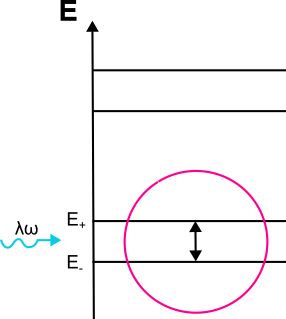
\includegraphics[width=0.4\textwidth]{twolevel} % Replace 'example-image' with your file name
\end{wrapfigure}

Ipotizziamo di mandare una radiazione la cui frequenza \`e all'incirca pari a quella che separa i due livelli energetici. Per descrivere l'elettrone che passa da un livello inferiore a quello superiore \`e sufficiente concentrarsi sui due livelli d'interesse in quanto gli altri livelli non rientrano nell'osservazione del fenomeno fisico. 

Matematicamente questo equivale a troncare lo spazio di Hilbert complessivo ad un sottospazio di dimensione finita. 

\begin{equation*}
	\mathcal{H} \to \mathbb{C}^n 
\end{equation*}
\vspace{0.3cm}


Nello spazio di Hilbert ridotto l'equazione di Schr\"odinger  assume una forma matriciale, dove la Hamiltoniana $H \in \text{Mat}_{n \times n}(\mathbb{K})$ e la funzione d'onda di conseguenza $|\psi \rangle \in \mathbb{K}^n$.
\newline

Gli esempi di sistemi approssimabili a sistemi a due livelli sono molteplici a partire da sistemi in cui la distanza di split medio tra due livelli \`e molto pi\`u piccola rispetto agli altri. Solitamente tali split sono associati a delle simmetrie del sistema. Un altro esempio \`e dato dalle oscillazioni del neutrino.

\subsection{Hamiltoniana in due stati}

Consideriamo un sistema fisico il cui spazio degli stati \`e rappresentabile da un insieme di bi-dimensionale. Come base del sistema consideriamo i due autostati $|\varphi_1 \rangle $ e $|\varphi_2 \rangle $ della Hamiltoniana $H_0$ e i cui rispettivi autovalori sono dai da $E_1$ e $E_2$:
\newpage 

\begin{equation}
H_0 |\varphi_1 \rangle = E_1 |\varphi_1 \rangle \quad \quad H_0 |\varphi_2 \rangle = E_2 |\varphi_2\rangle 
\end{equation}
Un generico stato \`e espresso come
\begin{equation*}
	|\psi \rangle = c_1(t)|\varphi_1 \rangle + c_2(t) |\varphi_2 \rangle 
\end{equation*}
dove ipotizziamo che gli autostati siano ortonormali tra loro
\begin{equation*}
	\langle \varphi_i | \varphi_j \rangle = \delta_{ij} \quad i,j = 1,2
\end{equation*}
I coefficienti dipendenti dal tempo sono soluzione dell'equazione di Schr\"odinger in forma matriciale 

\begin{equation*}
	i \hbar  \frac{d}{dt}\left ( \begin{array}{c} c_1(t) \\ c_2(t) \end{array}\right) = \left [ \begin{array}{cc} 
		H_{11} & H_{12} \\ H_{21} & H_{22}
	\end{array}\right ] \left ( \begin{array}{c} c_1(t) \\ c_2(t) \end{array}\right) 
\end{equation*}
dove gli elementi della matrice Hamiltoniana sono dati dalla relazione
\begin{equation}
	H_{ij} = \langle \varphi_i|\hat{H}|\varphi_j \rangle 
\end{equation}
La matrice della Hamiltoniana H \`e data dalla somma di una matrice $H_0$ che descrive il sistema nello stato iniziale e privo di perturbazione e $W$ che descrive la perturbazione (o l'accoppiamento) ed \`e una matrice Hermitiana.
\begin{equation*}
	H =H_0 + W = \left [ \begin{array}{cc}
		E_1 & 0 \\ 0 & E_2 
	\end{array}\right] + \left [ \begin{array}{cc}
	W_{11} & W_{12} \\ W_{21} & W_{22}
	\end{array}\right ]  = \left [ \begin{array}{cc} 
		H_{11} & H_{12} \\ H_{21} & H_{22}
	\end{array}\right ] 
\end{equation*}
\subsection{Soluzioni stazionarie}
Dalla relazione (4.15) insieme a (4.16) avremo che $H_{11} = E_1$ e $H_{22} = E_2$, per ipotesi iniziali.
Per determinare le soluzioni stazionarie del problema (autovettori) che rappresentano gli stati ad energia costante, le autofunzioni sono della forma
\begin{equation*}
	\left( \begin{array}{c}
	c_1(t) \\
	c_2(t)	
	\end{array}\right) = e^{-iEt / \hbar} \left( \begin{array}{c}
	c_1 \\
	c_2	
	\end{array}\right )
\end{equation*} 
I coefficienti indipendenti dal tempo e le energie sono dati dati da 
\begin{equation}
	\left [ \begin{array}{cc} 
		E_{1} & H_{12} \\ H_{21} & E_{2}
	\end{array}\right ] \left( \begin{array}{c} c_1 \\ c_2 \end{array}\right) = E \left ( \begin{array}{c} c_1 \\ c_2 \end{array}\right) 
\end{equation}
Per calcolare gli autovalori calcoliamo le radici del polinomio caratteristico associato $P(E) = \text{det}(H-EI) = 0$
\begin{equation*}
	\text{P(E)} = \text{det}	\left [ \begin{array}{cc} 
		E_{1}-E & H_{12} \\ H_{21} & E_{2}-E
	\end{array}\right ] = E^2 - E(E_1+E_2) +E_1E_2 - H_{12}H_{21} = 0
\end{equation*}
\newpage

essendo che la matrice \`e Hermitiana avremo che $H_{12} = H_{21}^*$, e dunque $H_{12}H_{21} =|H_{12}|^2$ di conseguenza le auto-energie del sistema sono date da 
\begin{align*}
	E_- = \frac{E_1 + E_2}{2} - \sqrt{\left( \frac{E_2 - E_1}{2}\right)^2 + |H_{12}|^2}\\[0.5cm]
	E_+ = \frac{E_1 + E_2}{2} + \sqrt{\left( \frac{E_2 - E_1}{2}\right)^2 + |H_{12}|^2}
\end{align*}

\begin{wrapfigure}{l}{0.4\textwidth} % r for right, l for left
    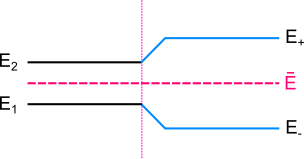
\includegraphics[width=\linewidth]{coupling} % Replace 'example-image' with your image file
    \caption{}
\end{wrapfigure}
\vspace{0.3cm}
In assenza di un fattore di perturbazione, $E_1$ e $E_2$ rappresentano i possibili stati dell'energia, e gli stati $|\psi_1 \rangle $ e $|\psi_2 \rangle$ sono stati stazionari (se il sistema assume una delle due configurazioni questo rimane in tale condizione indefinitivamente). Quondo si introduce una perturbazione $W$ gli stati di energia si modificano e dunque $|\varphi_1 \rangle , |\varphi_2 \rangle, E_1$e $E_2$ non sono pi\`u autovalori e autostati della Hamiltoniana $H$ che rappresenta il sistema perturbato, ma diventano $ |\varphi_{+}\rangle ,|\varphi_{-} \rangle  ,E_{+}$ e $E_{-}$.

Sostituendo gli autovalori trovati nella matrice (4.17) determiniamo gli autovettori associati
\begin{equation*}
		\left [ \begin{array}{cc} 
		E_{1} & H_{12} \\ H_{21} & E_{2}
	\end{array}\right ]\left( \begin{array}{c} c_1^{\pm} \\ c_2^{\pm} \end{array}\right) = E_{\pm} \left ( \begin{array}{c} c_1^{\pm} \\ c_2^{\pm} \end{array}\right) 
\end{equation*}
che ci porta all'equazione
\begin{equation*}
	H_{21}c_{1}^{\pm} +(E_2-E_{\pm})c_{2}^{\pm} = 0
\end{equation*}
che porta alle soluzioni normalizzate 
\begin{equation*}
	\left( \begin{array}{c} c_1^{\pm} \\ c_2^{\pm} \end{array}\right) = \frac{1}{\sqrt{1 + \left ( \frac{H_{21}}{E_{\pm} - E_2}\right)}}\left( \begin{array}{c} 1 \\ \frac{H_{21}}{E_{\pm} - E_2} \end{array}\right)
\end{equation*}
Possiamo semplificarne l'algebra definendo i termini 
\begin{equation*}
	\overline{E} = \frac{E_1 + E_2}{2} \quad \text{e} \quad \Delta  = \frac{E_2 - E_1}{2}
\end{equation*}
e posto $H_{12} = H_{21}^* = A$, avremo che 
\begin{equation*}
	\hat{H} = \left [ \begin{array}{cc}
		\overline{E} - \Delta & V \\ V^* & \overline{E}+ \Delta 
	\end{array}\right ] 
\end{equation*}
e
\begin{align*}
	E_- = \overline{E} - \sqrt{\Delta^2 + |V|^2} \quad \quad 	E_+ = \overline{E} + \sqrt{\Delta^2 + |V|^2}
\end{align*}
\newpage
Gli autovettori associati vengono riscritti nel seguente modo 
\begin{equation*}
	\binom{c_1^{-}}{c_2^{-}}=\frac{1}{\sqrt{V^2+\left(\Delta+\sqrt{\Delta^2+V^2}\right)^2}}\binom{\Delta+\sqrt{\Delta^2+V^2}}{-V}=\binom{\cos \theta}{\sin \theta}
\end{equation*}
e
\begin{equation*}
	\binom{c_1^{+}}{c_2^{+}}=\frac{1}{\sqrt{V^2+\left(-\Delta+\sqrt{\Delta^2+V^2}\right)^2}}\binom{-\Delta+\sqrt{\Delta^2+V^2}}{+V}=\binom{-\sin \theta}{\cos \theta}
\end{equation*}
dove 
\begin{equation*}
	\sin 2 \theta=-\frac{V}{\sqrt{\Delta^2+V^2}} \quad \text { e } \quad \cos 2 \theta=\frac{\Delta}{\sqrt{\Delta^2+V^2}}
\end{equation*}
In conclusione le auto funzioni soluzione dell'equazione di Schr\"odinger rispetto alla base di partenza $\{|\varphi_1 \rangle , |\varphi_2 \rangle \}$ sono date da 
\begin{equation*}
	|\psi_- \rangle = \cos\theta |\varphi_1 \rangle + \sin \theta |\varphi_2 \rangle 
\end{equation*}
e 
\begin{equation*}
	|\psi_{+} \rangle = - \sin \theta |\varphi_1 \rangle + \cos \theta |\varphi_2 \rangle 
\end{equation*}
La soluzione generale della funzione d'onda ad un tempo t, $|\psi(t) \rangle $ , la si determina dalla conoscenza dello stato iniziale del sistema descritto da $|\psi(0) \rangle $ ed espresso rispetto le funzione d'onda del sistema nello stato iniziale date da $|\varphi_+ \rangle $ e $|\varphi_- \rangle $. La funzione d'onda al tempo $t$ \`e dunque data da 
\begin{equation*}
	\psi(t)=c_{-} \psi_{-} e^{-i E_{-} t / \hbar}+c_{+} \psi_{+} e^{+i E_{+} t / \hbar}
\end{equation*}
dove $c_- = \langle \varphi_- | \psi(0) \rangle $ e $c_+ = \langle \varphi_+ |\psi(0) \rangle $.
\newline

\noindent Osserviamo che la presenza di una perturbazione nel sistema allarga i livelli di energia del sistema imperturbato, come si vede dalla figura 4.2; possiamo stimare la distanza tra le energie del sistema imperturbato e quello perturbato per valori di $|H_{12}|^2 = |A|^2$ non troppo grandi rispetto alle scale di energie del problema.

Definiamo 
\begin{align*}
E_{\pm}= & \; \frac{1}{2}\left(E_1+E_2\right)\pm \frac{1}{2} \sqrt{\left(E_1-E_2\right)^2+4\left|A\right|^2} = \\[0.5cm]
 = & \; \frac{E_1 + E_2}{2} \pm \frac{E_2 -E_1}{2} \sqrt{1 + \frac{4|A|^2}{(E_2-E_1)^2}}
\end{align*}
se consideriamo infinitesimo il secondo addendo sotto radice, ovvero $E_2 \simeq E_1$, possiamo sviluppare la radice usando il polinomio di Taylor, ottenendo
\begin{equation*}
	E_{\pm} = \frac{E_2 +E_1}{2} \pm \frac{E_2-E_1}{2} \left ( 1 + \frac{2|A|^2}{(E_2-E_1)^2}+ ...\right) 
\end{equation*}
e dunque possiamo approssimare gli stati $E_+$ e $E_-$ come 
\newpage

\begin{align*}
E_+ = E_2 + \frac{|A|^2}{(E_2-E_1)} \\[0.5cm]
E_- = E_1 - \frac{|A|^2}{(E_2- E_1)}	
\end{align*}
di conseguenza gli allargamenti energetici saranno quadratici in $|A|$. Dato che al denominatore \`e presente il termine $E_2-E_1$ esiste un caso speciale per quando $E_2 = E_1$, ovvero si ha degenerazione. In questo caso 
\begin{align*}
	E_+ = \overline{E} + |A| \\[0.5cm]
	E_- = \overline{E} - |A|
\end{align*}
dunque quando i livelli energetici sono degeneri tendono ad allargarsi linearmente in $|A|$ anzinch\`e quadraticamente. Nel caso in cui $|A|$ sia piccolo rispetto al problema, in caso degenerazione avremo un allargamento maggiore rispetto a quello prodotto da $|A|^2$ in caso di non degenerazione.

\subsection{Oscillazione del sistema tra due stati imperturbati: Formula di Rabi}

Supponiamo che il sistema si trovi inizialmente nello stato $|\psi(0)\rangle = |\varphi_1 \rangle $, che non \`e un auto stato del sistema, e lo sviluppiamo rispetto ai ket $\{|\varphi_+\rangle , |\varphi_- \rangle \}$. I coefficienti sono dati da $c_- = \cos \theta$ e $c_+ = - \sin \theta$, 
\begin{equation*}
	|\psi(0) \rangle  = -\sin\theta |\varphi_+ \rangle + \cos \theta |\varphi_- \rangle 
\end{equation*}
applicando l'operatore di evoluzione temporale, avremo che l'evoluto al tempo $t$ \`e dato da 
\begin{equation*}
	|\psi(t) \rangle =-e^{-iE_+ t/ \hbar}\sin{\theta}|\varphi_+ \rangle   + \cos\theta e^{-iE_-t/\hbar}|\varphi_- \rangle 
\end{equation*}
che possiamo esprimere rispetto alla base del sistema imperturbato come 
\begin{equation*}
	|\psi(t) \rangle =\left[\cos ^2 \theta e^{-i E_{-} t / \hbar}+\sin ^2 \theta e^{-i E_{+} t / \hbar}\right] |\varphi_1 \rangle +\sin \theta \cos \theta\left[e^{-i E_{-} t / \hbar}-e^{-i E_{+} t / \hbar}\right] |\varphi_2\rangle 
\end{equation*}
la probabilit\`a che il sistema si trovi nello stato $|\varphi_2 \rangle $ \`e data da 
\begin{equation*}
	P_{12}(|\psi(t) \rangle = |\varphi_2 \rangle) = |\langle \varphi_2| \psi(t) \rangle|^2 = 4\sin ^2 \theta \cos ^2 \theta \sin ^2 \left ( \frac{\sqrt{\Delta^2+V^2} t }{ \hbar} \right)
\end{equation*}
usando il risultato $2 \sin(\theta) \cos(\theta) = \sin(2 \theta)$, possiamo riscrivere la probabilit\`a come 
\begin{equation*}
 P_{12}(t) = \frac{V^2}{\Delta^2 + V^2}\sin^2 \left (\frac{\sqrt{\Delta^2 + V^2}\;t}{\hbar} \right )
\end{equation*}
Nel caso in cui abbiamo dei livelli di energia degeneri in cui $E_1 = E_2$ la probabilit\`a assume la forma 
\newpage 
\begin{equation*}
	P_{12}(t) = \sin^2 \left(\frac{|V|\;t}{\hbar}\right)
\end{equation*}
 
\begin{figure}[!ht]
\vspace{0.1in}
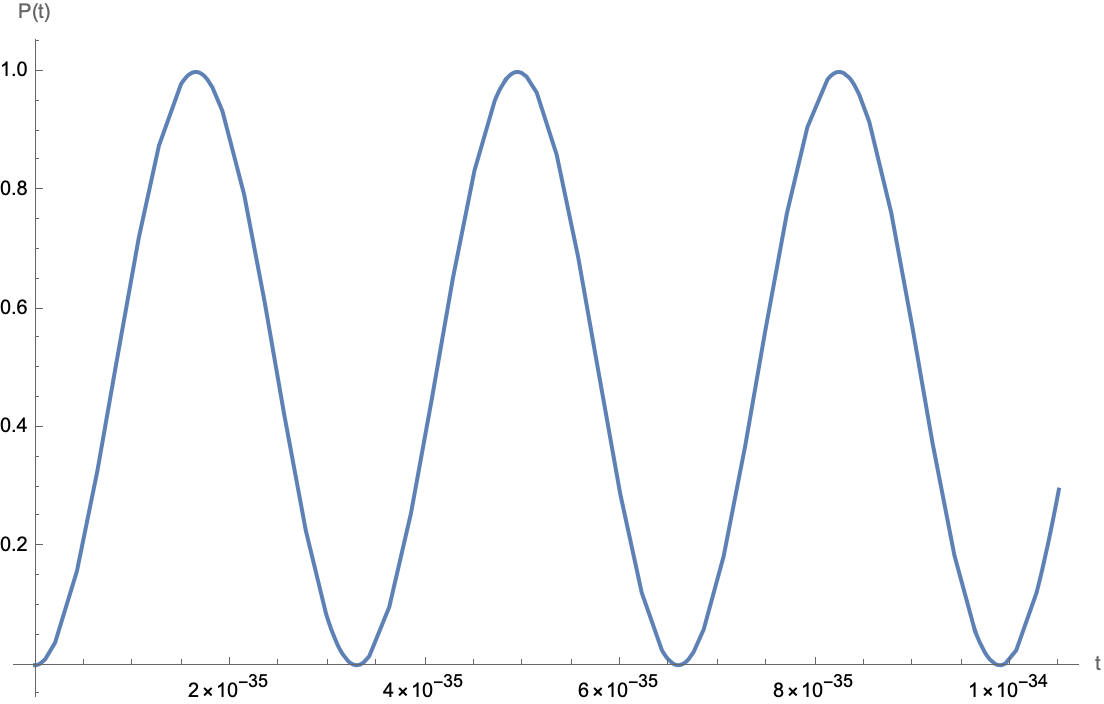
\includegraphics[width = 8.5cm]{degencoupling}	
\centering
\vspace{0.1in}
\caption{Probabilit\`a di trovarsi nello stato $|\varphi_2 \rangle $ per un energia degenere $E_1 =E_2$}
\end{figure}

\noindent La particella oscilla tra i due stati con certo periodo, con una frequenza $\omega = \frac{2|A|}{\hbar}$
che \`e legato alla perturbazione applicata.
\newline

Nel caso in cui $E_1 \neq E_2$ la particella oscilla tra i due stati con una frequenza 
\begin{equation*}
	\omega = \frac{2 \sqrt {\Delta^2 +V^2}}{\hbar} = \frac{E_+ -E_-}{\hbar}
\end{equation*}
che coincide con la frequenza di Bohr, associata allo splitting di due libelli energetici. Possiamo riscrivere la probabilit\`a che il sistema si trovi nello stato $|\varphi_2 \rangle$ nel seguente modo
\begin{equation*}
	P_{12}(t) = \underbrace{\frac{4|V|^2}{\hbar^2} \left [ (\Delta \omega)^2 + \frac{4|V|^2}{\hbar^2	}\right ]^{-1}}_{ = \alpha} \sin^2 \left( \sqrt{\Delta \omega^2 + \frac{4|V|^2}{\hbar^2}} \frac{\hbar}{2} \right)
\end{equation*}
dove 
\begin{equation*}
	\Delta\omega = \frac{E_2 - E_1}{\hbar}
\end{equation*}
che definisce lo splitting dei livelli prima della perturbazione del sistema. Se si hanno dei livelli distinti di energia si ha una scala data dalla differenza di energia tra i due livelli, quindi possiamo chiederci se la perturbazione \`e molto pi\`u piccola o grande della differenza di energia tra i due livelli.  Se la perturbazione \`e molto pi\`u piccola della differenzia di energia tra i due livelli, ci aspettiamo che la probabilit\`a massima sia piccola, ovvero esiste una bassa probabilit\`a che il sistema passi da uno stato energetico all'altro.
\newpage 


\subsection{Perturbazione per un potenziale dipendente dal tempo }

Supponiamo che la perturbazione introdotta nel sistema dipenda in modo monocromatico dal tempo con una frequenza data $\omega$, la Hamiltoniana del sistema perturbato \`e espressa nel seguente modo:
\begin{equation*}
	H(t) = \left [ \begin{array}{cc}
		E_1 & A^*e^{i\omega t} \\
		Ae^{-i\omega t} & E_2 \\ 
	\end{array} \right ]
\end{equation*}

L'equazione di Schr\"odinger associata pu\`o \`e data da 
\begin{equation*}
	i  \hbar \frac{d}{dt} \left[ \begin{array}{c}
		a(t) \\ b(t)
	\end{array}\right ]  = \left [\begin{array}{cc}
	\begin{array}{cc}
		E_1 & A^*e^{i\omega t} \\
		Ae^{-i\omega t} & E_2 \\ 
	\end{array}
	\end{array}\right ] \left[ \begin{array}{c}
		a(t) \\ b(t)
	\end{array}\right ]
\end{equation*}
e pu\`o essere risolta esattamente, per farlo consideriamo un cambio di variabile
\begin{equation*}
	a(t) = \overline{a}(t) e^{i \omega t /2}  \quad \text{e} \quad b(t) = \overline{b}(t)e^{-i\omega t/2}
\end{equation*}
In questo modo abbiamo un sistema di equazioni differenziali al primo ordine 
\begin{equation*}
	\left \{ \begin{array}{l}
		i \hbar \dot{\overline{a}} = \left ( E_1 + \frac{\hbar \omega}{2}\right) \overline{a} + A^*\overline{b} \\[0.5cm]
		i \hbar \dot{\overline{b}} = A \overline{a} + \left ( E_2 + \frac{\hbar \omega}{2}\right)\overline{b}
	\end{array}\right.
\end{equation*}
il problema non dipende pi\`u dal tempo e ne conosciamo gi\`a la risoluzione, che coincide con quella vista per gli stati stazionari. Dove 
\begin{equation*}
	E_1 \to E_1 + \frac{\hbar \omega}{2} \quad \text{e} \quad E_2 \to E_2 + \frac{\hbar \omega}{2}
\end{equation*}
dato che $\Delta E = E_2 - E_1  - \hbar \omega$ nell'equazione stazionaria andremo a sostituire $\Delta \omega $ con $\Delta \omega - \omega$ e in conclusione la probabilit\`a che il sistema si trovi nello stato $|\varphi_2 \rangle$ \`e data da 
\begin{equation*}
	P_{12}(t) = \frac{4|A|^2/ \hbar^2}{(\Delta \omega - \omega)^2 + 4|A|^2/\hbar^2} \sin^2 \left ( \sqrt{(\Delta \omega - \omega)^2 + \frac{4|A|^2}{\hbar^2} }\frac{t}{\hbar} \right)
\end{equation*}
che prende il nome di \textit{formula di Rabi generalizzata}.

Da un punto di vista fisico possiamo interpretare il risultato come la differenze dei livelli di energia meno la frequenza della perturbazione, che pu\`o essere data da dei fotoni (radiazione) che perturbano un atomo con due livelli energetici. Si osserva che la probablit\`a \`e sempre pi\`u piccola di 1 a meno che $\Delta \omega = \omega$, ovvero nel caso in cui ritroviamo la formula di Bohr $E_2 - E_1 = \hbar \omega $.

\subsection{Esempio di Sistema a due Livelli}

Consideriamo un potenziale della forma $V(x) = (x^2-x_0)^2$, e dunque dato da una funzione pari che classicamente corrisponde ad avere due stati a minima energia equivalenti.
\newpage 

\begin{figure}[!ht]
\vspace{0.1in}
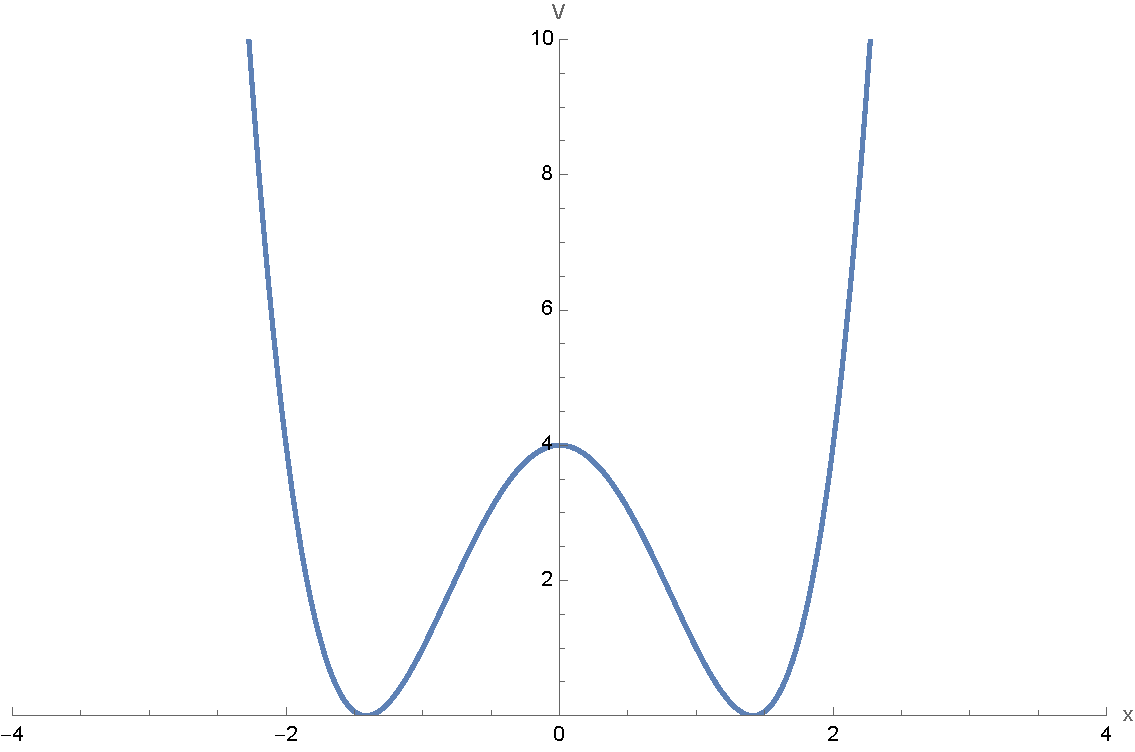
\includegraphics[width = 9cm]{quartic}	
\centering
\vspace{0.1in}
\caption{Esempio di potenziale quartico $V(x) = (x^2-2)^2$}
\end{figure}

In meccanica quantistica i due stati che classicamente sono di energia minima corrispondono a due stati degeneri, dato che sono coincidenti. Se per\`o il potenziale \`e mono dimensionale regolare ed illimitato  lo stato fondamentale del sistema \`e non degenere. 

Il problema diventa equivalente a due oscillatori armonici, dati dalle due buche di potenziale. Per simmetria dovremmo calcolare solo i livelli di energia di uno degli oscillatori armonici per buca di potenziale, solo che le auto funzioni sono invarianti per parit\`a $x \to -x$, ma non in modo banale. Dato che nel passaggio da una buca all'altra di ha un potenziale di altezza finita, se si cerca di costruire una funzione d'onda che assomigli allo stato fondamentale dell'oscillatore armonico per $x$ in prossimit\`a di $x_0$, si genera un effetto tunnel, ovvera si ha una probabilit\`a non nulla di passare da una parte all'altra.

\subsubsection{Soluzione qualitativa del problema}

Consideriamo il caso in cui la barriera \`e molto alta e quindi possiamo considerare le buche  disaccopiate. La Hamiltoniana che descrive il sistema a due livelli perturbato \`e data da 
\begin{equation*}
	H = \left [\begin{array}{cc}
		E & - A \\
		-A & E
	\end{array}\right ]
\end{equation*} 
I termini off-diagonali introducono un un'ampiezza di transizione tra lo stato nella prima buca  e lo stato nella seconda buca. Avremo di conseguenza lo split di uno stato di partenza degenere. 

Osserviamo che la Hamiltoniana che descrive il sistema pu\`o essere riscritta rispetto alla matrice di Pauli $\sigma_1$ nel seguente modo
\begin{equation*}
	H = EI - A \sigma_1
\end{equation*}
di conseguenza gli autovettori sono combinazione di lineare quelli di $\sigma_1$
\begin{equation*}
	|\pm \rangle = \frac{1}{\sqrt{2}}\left [\begin{array}{c}
		1 \\ \pm 1
	\end{array} \right ]  = \frac{|1 \rangle \pm |2\rangle }{\sqrt{2}}
\end{equation*}
\newpage 
\begin{figure}[ht]
    \begin{minipage}[b]{0.45\linewidth}
        \centering
        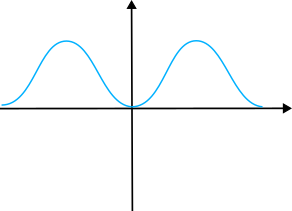
\includegraphics[width=\linewidth]{firststate}
        \caption{$\frac{|1\rangle + |2\rangle }{\sqrt{2}}$}
    \end{minipage}
    \hspace{0.1\linewidth}
    \begin{minipage}[b]{0.45\linewidth}
        \centering
        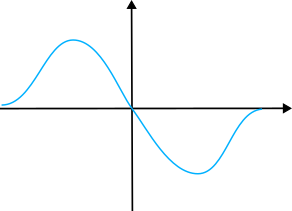
\includegraphics[width=\linewidth]{secondstate}
        \caption{$\frac{|1\rangle - |2\rangle }{\sqrt{2}}$}
    \end{minipage}
\end{figure}
Per un moto monodimensionale gli stati fondamentali tendono ad avere il numero minore possibile di punti in cui si annullano. Dato che in $(|1 \rangle - |2 \rangle)/\sqrt{2}$ abbiamo uno zero della funzione d'onda ci aspettiamo che nel sistema perturbato questo coincida con lo stato eccitato.

In problemi di questo tipo la simmetria classica si rompe, in quanto \`e presente sia uno stato a minima energia non degenere che uno stato eccitato in cui la particella \`e simultaneamente  presente in tutte e due le buche. Nel caso dello stato degenere la differenza \`e definita a meno di un fattore di fase.

\subsection{La molecola di ammoniaca $NH_3$ come sistema a due stati}
\begin{wrapfigure}{r}{0.4\textwidth} % r for right, l for left
    \centering
    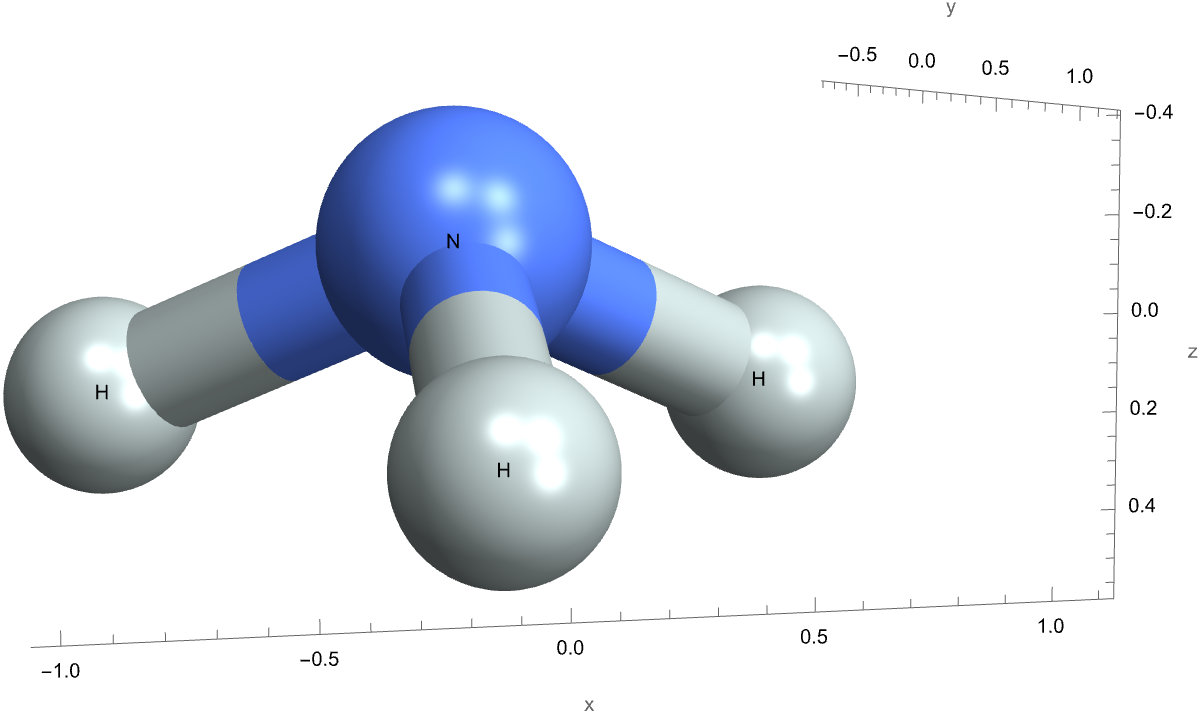
\includegraphics[width=0.38\textwidth]{ammonia1} % Adjust width as needed
\end{wrapfigure}
La molecola di ammoniaca $NH_3$ \`e composta da quattro atomi, tre di idrogeno e uno di azoto e assume la forma di un tetraedro schiacciato dove i tre atomi di idrogeno formato la base triangolare e quello di azoto la punta. La molecola pu\`o trovarsi in due stati possibili dovuti alla transizione in cui l'atomo di azoto posto in cima al tetraedro viene ruotato finendo al di sotto del piano formato dalla base triangolare con ai vertici gli atomi di idrogeno. 
\begin{figure}[!ht]
\vspace{0.1in}
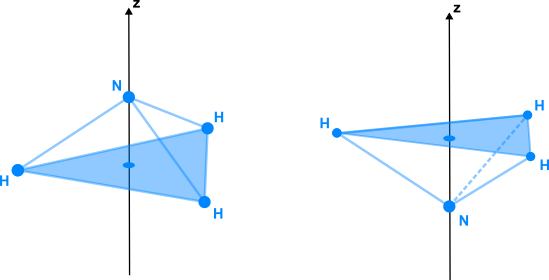
\includegraphics[width = 10cm]{ammoniaRotation}	
\centering
\vspace{0.1in}
\caption{I due stati possibili della molecola di ammoniaca.}
\end{figure}
\newpage

Il passaggio da uno stato all'altro pu\`o essere descritto da una rotazione della molecola. Possiamo descrivere la transizione da un punto di vista fisico considerando la rotazione della molecola attorno all'asse ortogonale alla base del tetraedro formata dall'idrogeneo, con N verso l'alto, dove la direzione verso l'alto \`e data dalla direzione del momento angolare. Analogamente la configurazione in N \`e verso il basso, si ha che il basso \`e dato dalla direzione opposta a quella del momento angolare della molecola.

In meccanica classica i due stati possibili dell'ammoniaca sono degeneri rispetto l'energia. In meccanica quantistica se la barriera di potenziale \`e finita, la degenerazione dell'energia pu\`o essere spezzata. Un potenziale V(z) dato da un polinomio di quarto grado rappresenta il potenziale di configurazione della molecola di ammoniaca, inoltre possiede due punti di minimo che definiamo come $\pm z_0$ e che sono separati tra loro da una barriera molto larga.

\begin{figure}[!ht]
\vspace{0.1in}
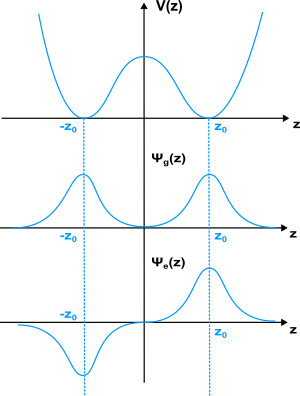
\includegraphics[width = 7cm]{ammoniaState}	
\centering
\vspace{0.1in}
\caption{V(z) rappresenta il potenziale a cui \`e soggetta la molecola di ammoniaca. Sono presenti due posizioni di equilibrio in senso classico $\pm z_0$. Al di sotto del potenziale sono rappresentati $\psi_g$ che descrive lo stato fondamentale e $\psi_{e}$ per il primo stato eccitato.}
\end{figure}
In un potenziale di questo tipo lo stato fondamentale, che \`e simmetrico, e il primo stato eccitato, che \`e antisimmetrico, sono quasi degeneri nell'energia quando la barriera \`e molto alta. Se la barriera di potenziale fosse infinita, i due possibili autostati sarebbero dati dalla funzione d'onda che descrive la posizione dell'azoto in $z_0$ e da quella che lo descrive nella posizione $-z_0$. Inoltre questi stati sarebbero degeneri rispetto l'energia. Nel nostro caso la barriera \`e larga, ma finita e quindi lo stato fondamentale \`e la funzione d'onda $\psi_g(z)$ rappresentata nella figura 4.8. 
  
La funzione $\psi_g(z)$ \`e combinazione lineare delle funzioni di stato che identificano la molecola nei due stati fondamentali possibili localizzati in $\pm z_0$. Si ha una funzione pari, somma di due stati locali con lo stesso segno. Analogamente la funzione $\psi_e(z)$ che rappresenta il primo stato eccitato \`e combinazione lineare di funzioni d'onda localizzate in $\pm z_0$ e con segni discordi, infatti si ha che $\psi_e(z)$ \`e una funzione dispari.

\subsubsection{Descrizione quantitativa}

Indichiamo i due stati possibili come 
\begin{equation*}
	|\uparrow \rangle \quad \text{l'azoto \'e su} \quad |\downarrow \rangle \quad \text{l'azoto \`e gi\`u} 
\end{equation*}
Possiamo associare a $|\uparrow \rangle $ una funzione d'onda positiva localizzata in intorno di $z_0$ e a $|\downarrow \rangle$ una funzione d'onda sempre positiva definita in un intorno di $-z_0$. Per ipotesi supponiamo che la barriera di energia sia infinita. In questo caso i due autostati hanno come autovalore il medesimo livello di energia $E_0$
\begin{equation*}
	H |\uparrow \rangle = E_0 |\uparrow \rangle \quad \text{e} \quad H|\downarrow \rangle = E_0 |\downarrow \rangle 
\end{equation*}
Definiamo i due stati 
\begin{equation*}
	|\uparrow \rangle \equiv |1 \rangle \quad \text{e} \quad |\downarrow \rangle \equiv |2 \rangle
\end{equation*}
come elementi della base della Hamiltonina H che assume la forma di una matrice $2 \times 2$
\begin{equation*}
	H = \left [\begin{array}{cc}
		E_0 & 0 \\ 0 & E_0
	\end{array} \right]
\end{equation*}
La possibilit\`a di avere un effetto tunnel che permette ai due stati di comunicare \`e espresso dagli elementi off-diagonali della matrice della Hamiltoniana e dunque gli elementi $H_{12} = \langle 1|H|2\rangle \neq 0$. Dato che l'operatore Hamiltoniano \`e Hermitiano abbiamo che $H_{12} = H_{21}^*$. Per ipotesi scegliamo dei termini off-diagonali reali 
\begin{equation*}
	H_{12} =H_{21} = - \Delta, \quad \Delta > 0
\end{equation*} 
il segno negativo \`e per convenzione. La Hamiltoniana che tiene conto degli effetti perturbativi dati dalla comunicazione dei due stati per via di una barriera di potenziale finita \`e 
\begin{equation*}
	H = \left [ \begin{array}{cc}
		E_0 & -\Delta \\ - \Delta & E_0 
	\end{array}\right ]=E_0\mathbb{I} - \Delta \sigma_1
\end{equation*}
dove $\sigma_1$ \`e la matrice di Pauli. Procediamo a calcolare gli autovalori dell'operatore Hamiltoniano diagonalizzando la matrice che lo rappresenta
\begin{equation*}
	\left [ \begin{array}{cc}
		E_0 - \lambda & -\Delta \\ -\Delta & E_0 - \lambda
	\end{array}\right] = 0 \quad \Rightarrow \quad (E_0 - \lambda)^2 = \Delta^2 \quad \Rightarrow \quad \lambda_{\pm} = E_0 \pm \Delta
\end{equation*}
Gli autostati corrispondenti agli autovalori sono
\begin{align}
	& |G \rangle = \frac{1}{\sqrt{2}} \left [ \begin{array}{c}
		1 \\ 1
	\end{array}\right ] = \frac{1}{\sqrt{2}}(|\uparrow \rangle + |\downarrow \rangle), \quad E = E_0 - \Delta, \quad \text{Stato fondamentale} \\
	& |E \rangle = \frac{1}{\sqrt{2}} \left [ \begin{array}{c}
		1 \\ -1
	\end{array}\right ] = \frac{1}{\sqrt{2}}(|\uparrow \rangle - |\downarrow \rangle), \quad E = E_0 + \Delta, \quad \text{Stato eccitato} 
\end{align}

Lo stato fondamentale $|G \rangle$ \`e sovrapposizione degli elementi della base con lo stesso segno, e analogamente lo stato eccitato $|E \rangle$, ma con segni opposti.

Lo stato eccitato \`e equivalente allo stato di spin $\frac{1}{\sqrt{2}}(|+ \rangle - |-\rangle)$ che punta nella direzione $-x$, mentre lo stato fondamentale corrisponde allo stato di spin $\frac{1}{\sqrt{2}}(|+ \rangle + |-\rangle)$ che punta nella direzione +x.

La differenza di energia tra i due autostati \`e $2 \Delta$, che per la molecola di ammoniaca ha valore
\begin{equation*}
	2 \Delta = 0.9872 \times 10^{-4} \;eV
\end{equation*} 
Se poniamo la differenza di energia uguale a quella di un fotone emesso durante la transizione si ha che 
\begin{equation*}
	2 \Delta = \hbar \omega = h \nu \quad \rightarrow \quad \nu = 23.870 \times 10^9 \; Hz =23.870 \;GHz
\end{equation*}
che corrisponde ad una lunghezza d'onda $\lambda$ 
\begin{equation*}
	\lambda = 1.2559 \;cm
\end{equation*}
Consideriamo l'evoluzione nel tempo della molecola di ammoniaca ipotizzando che al tempo $t = 0$ si trovi nello stato $|\uparrow \rangle$.  Utilizzando (4.18/19) lo stato iniziale \`e dato da 
\begin{equation*}
	|\Psi(0) \rangle = |\uparrow \rangle = \frac{1}{\sqrt{2}}(|G \rangle + |E \rangle)
\end{equation*}
e applicando l'operatore di evoluzione temporale si ha che lo stato al generico tempo $t$ \`e 
\begin{equation*}
	|\Psi(t) \rangle = \frac{1}{\sqrt{2}}(e^{-i(E-\Delta)t/\hbar}|G \rangle + e^{-i(E+\Delta)t/\hbar}|E \rangle )
\end{equation*}
che esplicitando i termini $|G \rangle$ e $|E \rangle $ abbiamo che l'equazione diventa 
\begin{equation*}
	\begin{aligned}
|\Psi, t\rangle & =\frac{1}{\sqrt{2}}\left(e^{-i(E-\Delta) t / \hbar} \frac{1}{\sqrt{2}}(|\uparrow\rangle+|\downarrow\rangle)+e^{-i(E+\Delta) t / \hbar} \frac{1}{\sqrt{2}}(|\uparrow\rangle-|\downarrow\rangle)\right), \\[0.5cm]
& =\frac{1}{2} e^{-i E t / \hbar}\left(e^{i \Delta t / \hbar}(|\uparrow\rangle+|\downarrow\rangle)+e^{-i \Delta t / \hbar}(|\uparrow\rangle-|\downarrow\rangle)\right), \\[0.5cm]
& =e^{-i E t / \hbar}\left[\cos \left(\frac{\Delta t}{\hbar}\right)|\uparrow\rangle+i \sin \left(\frac{\Delta t}{\hbar}\right)|\downarrow\rangle\right] .
\end{aligned}
\end{equation*}
Lo stato ottenuto dipendente dal tempo oscilla tra $|\uparrow \rangle$ e $|\downarrow \rangle $ con una frequenza angolare di $\omega = \Delta / \hbar \simeq 23  \;GHz$. La pobabilit\`a che la molecola di ammoniaca si trovi nello stato con azoto $| \uparrow \rangle $ o $|\downarrow \rangle $ \`e data da 
\begin{equation*}
	\begin{aligned}
& P_{\uparrow}(t)=|\langle\uparrow \mid \Psi, t\rangle|^2=\cos ^2\left(\frac{\Delta t}{\hbar}\right), \\[0.5cm]
& P_{\downarrow}(t)=|\langle\downarrow \mid \Psi, t\rangle|^2=\sin ^2\left(\frac{\Delta t}{\hbar}\right) .
\end{aligned}
\end{equation*}
\newpage
 
\begin{figure}[!ht]
\vspace{0.1in}
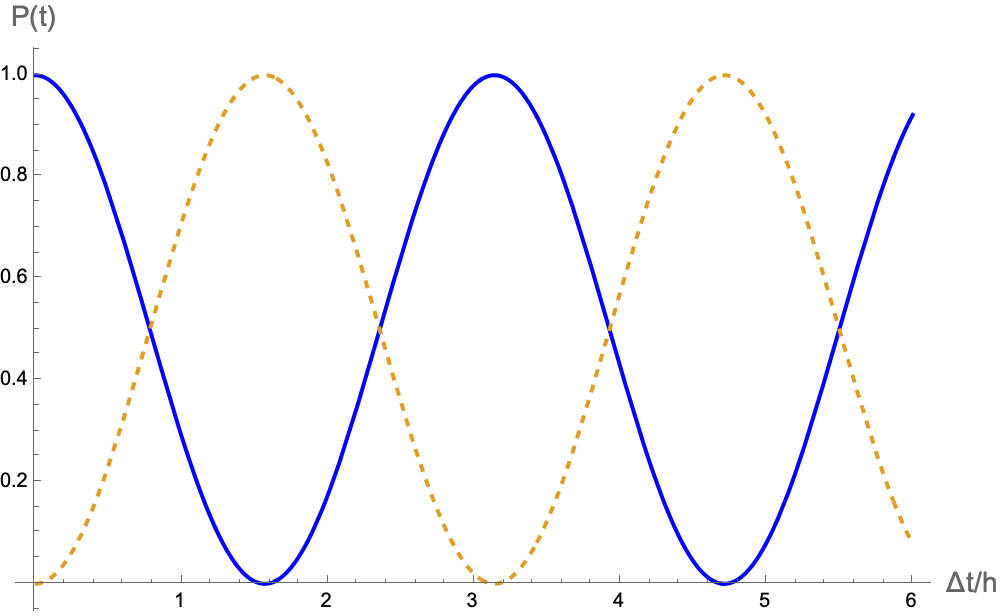
\includegraphics[width = 8cm]{ammonyProb}	
\centering
\vspace{0.3in}
\caption{Se l'atomo di azoto si trova nello stato iniziale $|\uparrow \rangle$ al tempo $t=0$  allora la probabilit\`a $P_{\uparrow}(t)$ (rappresentata come linea continua) oscilla tra zero e uno. La probabilit\`a che $P_{\downarrow}(t)$ che l'atomo di azoto si trova nello stato $|\downarrow \rangle$ \`e rappresentata dalle linee tratteggiate. Ovviamente $P_{\uparrow}(t) + P_{\downarrow}(t) =1$.}
\end{figure}

\subsection{Ione di idrogeno $H_2^+$ come sistema a due livelli}

\begin{wrapfigure}{r}{0.4\textwidth} % 'r' for right, width of the figure
    \centering
    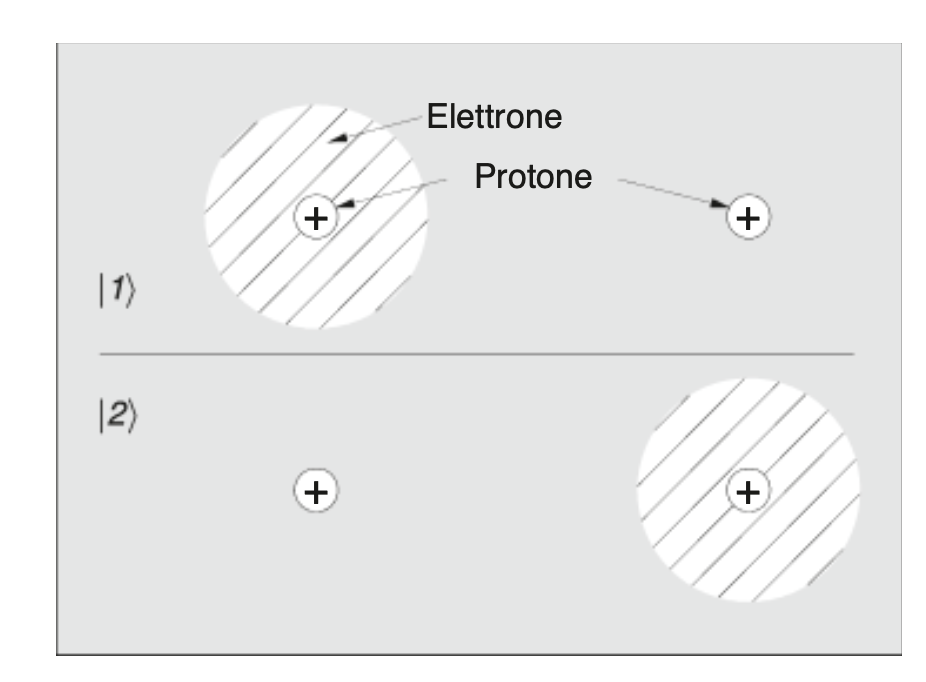
\includegraphics[width=0.38\textwidth]{ionHydrogen} % Replace with your image file
\end{wrapfigure}
Una molecola d'idrogeno ionizzato \`e data da due protoni ed un elettrone che si muove tra di essi. Quando i due protoni sono molto distanti tra loro l'elettrone rimane vincolato ad uno dei due formando un atomo d'idrogeno  al suo stato energetico  pi\`u basso. Dato che i protoni presenti nel sistema sono due, si hanno due possibili configurazioni simmetriche tra loro; ovvero se etichettiamo i due protoni come A e B, avremo che nello stato $|1 \rangle $  l'elettrone si legata al protone A e lascia ionizzato B, il viceversa identifica lo stato $|2 \rangle$.

A prescindere in quale dei due stati il sistema si trovi, l'energia di legame tra elettrone e protone \`e di $13,6 \; eV$ e corrisponde all'energia necessaria a strappare l'elettrone dal protone attorno a cui orbita. Fino a quando i due protoni sono sufficientemente distanti il protone "isolato" non ha sufficiente energia per slegare dell'elettrone dall'atomo d'idrogeno. 

Quanto discusso \`e trattato da un punto di vista classico che quindi ritiene impossibili la transizione di stato, ma da un punto di vista quantistico la probabili\`a di passaggio esiste anche se minima.  Entrambi gli stati $|1 \rangle$ e $|2 \rangle $ hanno energia $E_0$ e quindi la Hamiltoniana che descrive il sistema \`e 
\begin{equation*}
	\hat{H}_{0} = \left  [\begin{array}{cc}
		E_0 & 0 \\ 0 & E_0
	\end{array}\right]
\end{equation*}
La possibilit\`a di passaggio dell'elettrone da un protone all'altro introduce dei termini perturbativi -A all'interno della Hamiltoniana occupando gli spazi off-diagonali di $H_0$  e quindi la Hamiltoniana del sistema perturbato \`e data da
\newpage
\begin{equation*}
	\hat{H} = \left [ \begin{array}{cc}
		E_0 & -A \\ -A & E_0
	\end{array}\right]
\end{equation*}

Se consideriamo i due stati possibili trascurando la possibilit\`a che l'elettrone possa passare da uno stato all'altro questi si trovano alla medesima energia $E_0$. Proprio per la possibilit\`a di transizione di stato dell'elettrone abbiamo che i livello energetico si pu\`o separare i due livelli possibili. Maggiore sar\`a la separazione tra i due livelli e maggiore \`e la probabili\`a di transizione. Rispettivamente i due livelli energetici del sistema sono $E_0 + A$ e $E_0 -A$ associati agli stati 
\begin{align*}
	|I \rangle = \frac{1 }{\sqrt{2}}(|1 \rangle - |2 \rangle) \\[0.4cm]
	|II \rangle = \frac{1}{\sqrt{2}}(|1 \rangle + |2 \rangle)
\end{align*}
Il termine A all'interno della Hamiltoniana definisce l'ampiezza di probabilit\`a della transizione di stato dell'elettrone e questa dipende dalla distanza D tra i due protoni. Essa diminuisce esponenzialmente rispetto a D. 

Di conseguenza la probabili\`a aumenta all'aumentare della vicinanza tra i due protoni e quindi anche la separazione dei due livelli.

\begin{wrapfigure}{l}{0.4\textwidth} % 'r' for right, width of the figure
    \centering
    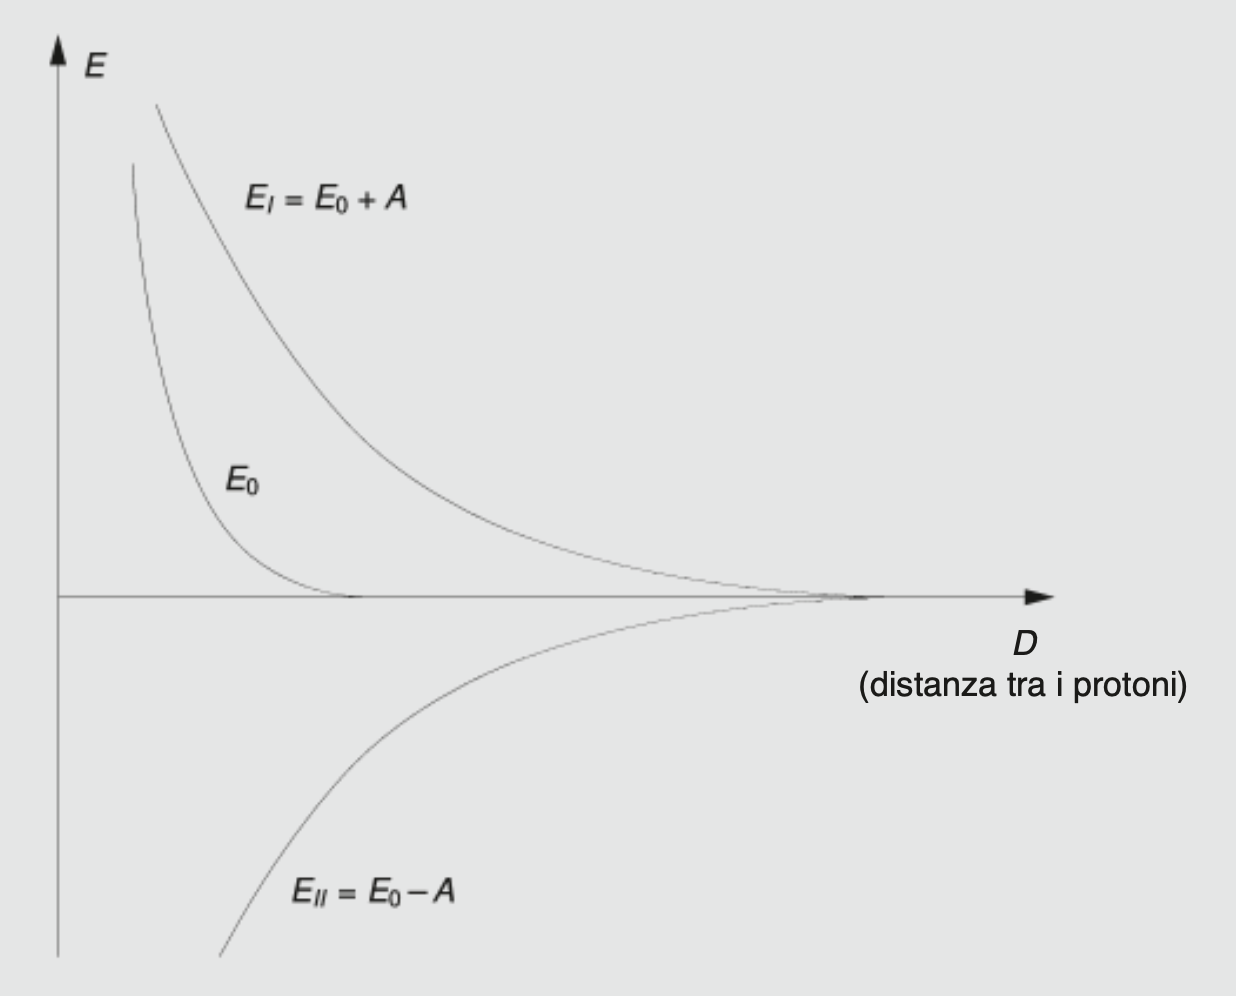
\includegraphics[width=0.38\textwidth]{energyhydro} % Replace with your image file
\end{wrapfigure}
Se il sistema di trova nello stato $|I \rangle$ l'energia $E_0 +A$ aumenter\`a al diminuire della distanza , gli effetti quantistici che descrivono l'interazione dell'elettrone con il protone "isolato" producono una forza di natura repulsiva che mantiene distanti i protoni. 
Partendo dalla stato $|II \rangle$ l'energia totale diminuisce quando i protoni si avvicinano e si ha una forza attrattiva tra i due protoni. 
In questo modo otteniamo una spiegazione delle forze di legame che tengono insieme lo ione $H_2^+$.

Oltre alle forze di legame dovute ai fenomeni quantistici si ha anche la presenza di una forza elettrostatica tra i due protoni, che risulta trascurabile a distanze sufficientemente grandi. Quando i due protoni sono molto vicini la forza di Coulomb influisce significativamente sul sistema e quindi fornisce un contributo energetico che deve essere incluso in $E_0$. Come conseguenza si ha che le energie di $E_{I}$ e $E_{II}$ varieranno in funzione della distanza interprotonica come in figura.
\newpage

\begin{wrapfigure}{r}{0.4\textwidth} % 'r' for right, width of the figure
    \centering
    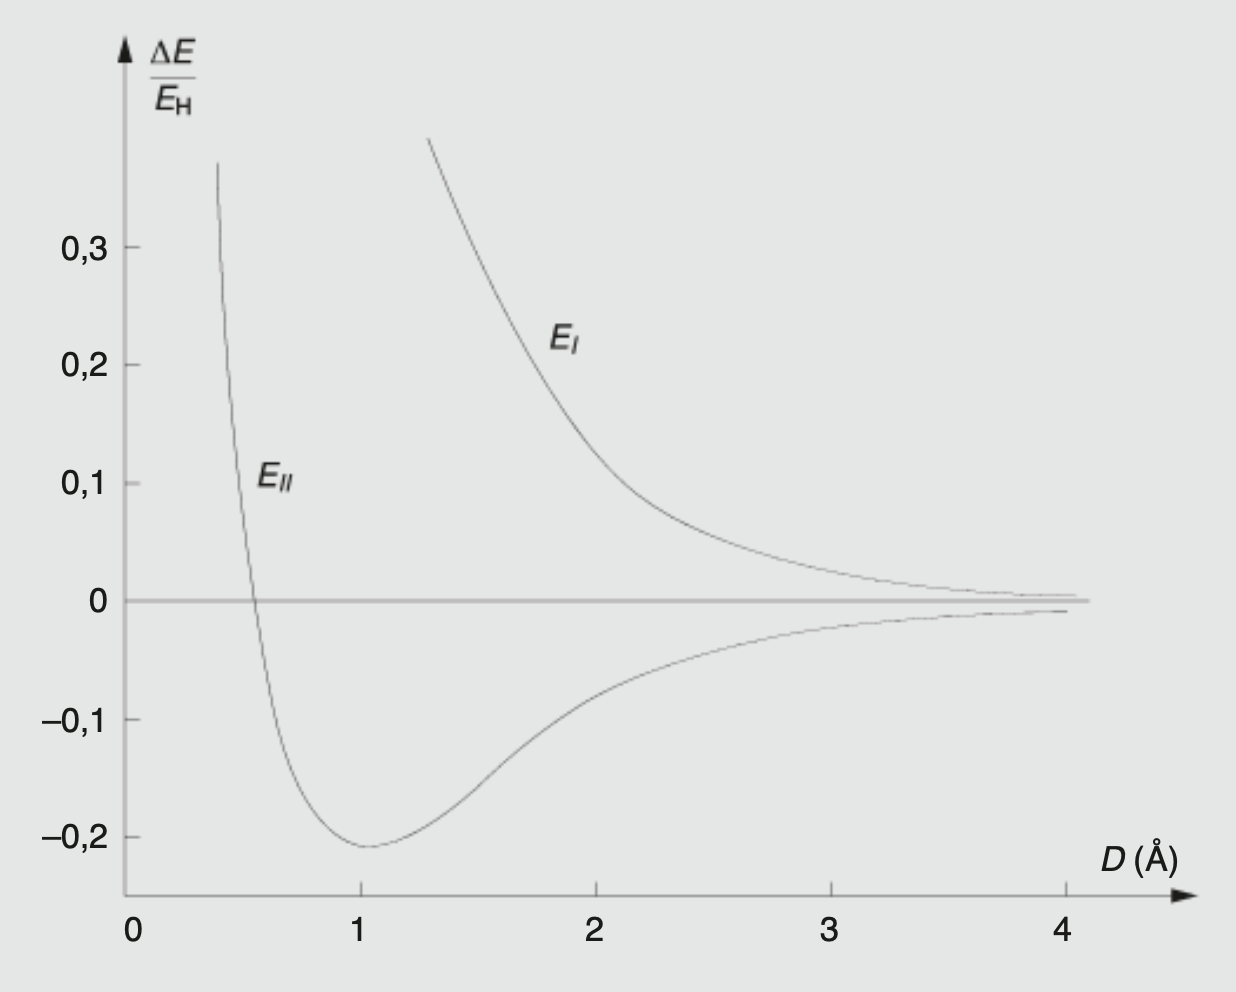
\includegraphics[width=0.38\textwidth]{energyhydro2} % Replace with your image file
\end{wrapfigure}
Lo stato $|II \rangle$  ha un punto di minimo dell'energia e rappresenta la configurazione di equilibrio per lo ione d'idrogeno, ovvero la condizione in cui l'energia del sistema \`e minima. L'energia in questo punto \`e minore di quella di un protone e di uno ione d'idrogeno separati e il sistema \`e perci\`o legato.

Se consideriamo un sistema in cui sono presenti due oggetti differenti anzich\`e i protoni, avremo che i due stati $|1 \rangle$ e $|2 \rangle$ non hanno pi\`u la medesima energia inziale se trascuriamo la possibilit\`a di transizione dell'elettrone, ovvero $E_1 \neq E_2$. Come conseguenza si ha uno splitting quadratico rispetto al termine perturbativo A.

\begin{remark}
In meccanica quantistica se si hanno delle simmetrie lo stato fondamentale \`e unico. 
\end{remark}

\section{Composizione dei momenti angolari}

\subsection{Prodotto tensoriale tra ket e spazi di Hilbert}

In meccanica quantistica il prodotto tensoriale \`e un operatore matematico che viene usato per combinare insieme spazi di Hilbert di diversa dimensione ottenendo un'unico spazio per il sistema composto. Per esempio, possiamo combinare gli spazi di Hilbert che descrivono due particelle distinte per ottenere un'unico spazio che descrive il sistema bi-particellare nel suo complesso; oppure si possono combinare momento orbital e spin di una singola particella.

Ipotizziamo di avere due particelle distinguibili prive di spin che etichettiamo come 1 e 2, i corrispettivi spazi vettoriali sono $\mathcal{E}_1$ e $\mathcal{E}_2$. Entrambi sono spazi delle funzioni d'onda in tre dimensione 
che descrivono lo stato delle singole particelle
\begin{align*}
	&\mathcal{E}_1 = \{\phi(\bold{r}), \text{particella 1}\}\\[0.4cm]
	&\mathcal{E}_2 = \{\chi(\bold{r}), \text{particella 2}\}
\end{align*}
Lo spazio delle funzione d'onda che descrivono il sistema combinato a due particelle \`e un altro spazio, ovvero lo spazio $\mathcal{E}$ delle funzione d'onda definite sullo spazio combinato a sei dimensioni delle configurazioni rispetto ($\bold{r}_1,\bold{r}_2)$:
\begin{equation*}
	\mathcal{E} = \{\psi(\bold{r}_1,\bold{r}_2) \}
\end{equation*}

Un caso speciale di una funzione d'onda che descrive un sistema a due particelle \`e quando questa \`e esprimibile come prodotto delle funzioni d'onda che descrivono i singoli oggetti
\begin{equation*}
	\psi(\bold{r}_1,\bold{r}_2) = \phi(\bold{r}_1)\chi(\bold{r}_2)
\end{equation*}
 In generale ogni funzione d'onda a due particelle pu\`o essere scritta come combinazione lineare del prodotto delle funzioni d'onda che descrivono le singole particelle. Se introduciamo la base $\{u_n(\bold{r})\}$ per lo spazio $\mathcal{E}_1$ e la base $\{v_m(\bold{r})\}$ per $\mathcal{E}_2$, allora una fuzione d'onda per un sistema a due particelle pu\`o essere espressa come 
 \begin{equation*}
 	\psi(\bold{r}_1,\bold{r}_{2}) = \sum_{n,m}c_{nm}u_{n}(\bold{r}_1)v_{m}(\bold{r}_2)
 \end{equation*}
 dove i termii $c_{nm}$ sono i coefficienti di espansione. In sostanza il prodotto degli elementi della base degli spazi a singola particella formano una base per lo spazio a due particelle. 
 
 Nella costruzione della nostra funzione d'onda dello spazio $\mathcal{E}$ possiamo desumere che $\mathcal{E}$ sia il \textit{prodotto tensoriale} degli spazi $\mathcal{E}_1$ e $\mathcal{E}_2$, e quindi \`e esprimibile come
 \begin{equation*}
 	\mathcal{E} = \mathcal{E}_1 \otimes \mathcal{E}_2
 \end{equation*}
 In senso lato, possiamo dire che lo spazio tensoriale ottenuto \`e lo spazio il cui span \`e dato dal prodotto delle funzioni d'onda dei singoli spazi costituenti.
 
 Oltre al prodotto di spazi vettoriali, possiamo definire lo spazio tra ket. Per esempio data $|\psi \rangle \in \mathcal{E}$, questa pu\`o essere scritta come 
 \begin{equation*}
 	|\psi \rangle = |\phi \rangle \otimes |\chi \rangle
 \end{equation*}
 Nella notazione fisica alcune volte l'operatore $\otimes$ non \`e espresso esplicitamente e si scrive $|\psi \rangle = |\phi \rangle |\chi \rangle $.
 
 Formalmente possiamo dire che dato lo spazio $\mathcal{E}_1$ la cui base \`e $\{|u_n \rangle\} $, e $\mathcal{E}_2$ con base $\{|v_{m} \rangle\}$. Il prodotto tensoriale $\mathcal{E}_1 \otimes \mathcal{E}_2$ ha una base data da $\{|u_n \rangle \otimes |v_m \rangle\} $. Se gli spazi $\mathcal{E}_1$ e $\mathcal{E}_2$ hanno una dimensione finita, allora anche $\mathcal{E}$ \`e finito dimensionale e ha dimensione
 \begin{equation*}
 	\text{dim} \,\mathcal{E} = (\text{dim} \,\mathcal{E}_1)(\text{dim} \,\mathcal{E}_2) 
 \end{equation*}
Similmente se $\mathcal{E}_1$ e $\mathcal{E}_2$ hanno dimensione l'insieme $\mathcal{E}$ \`e infinito dimensionale.
\subsection{Prodotto tensoriale di operatori}

Supponiamo di avere un operatore $\hat{A}_1$ che agisce sullo spazio vettoriale $\mathcal{E}_1$ e un altro operatore $\hat{A}_2$ che agisce su $\mathcal{E}_2$ e sia $\mathcal{E} = \mathcal{E}_1 \otimes \mathcal{E}_2$.  Possiamo definire un operatore $\hat{A}_1 \otimes \hat{A}_2$, la cui azione su un elemento di $\mathcal{E}$ \`e data da
\begin{equation}
	(\hat{A}_1 \otimes \hat{A}_2)(|\alpha \rangle_{1} \otimes |\beta \rangle_2) = (\hat{A}_1|\alpha \rangle_{1}) \otimes (\hat{A}_2|\beta \rangle_2)
\end{equation}
dove $|\alpha \rangle_1  \in \mathcal{E}_1$ e $|\beta \rangle_2 \in \mathcal{E}_2$. Dato che un qualsiasi vettore di $\mathcal{E}$ pu\`o essere espresso come combinazione lineare del prodotto tensoriale di vettori di $\mathcal{E}_1$ e $\mathcal{E}_2$, possiamo usare il principio di sovrapposizione per estendere l'equazione (4.20)  definendo un azione di $\hat{A}_1 \otimes \hat{A}_2$ su un generico elemento di $\mathcal{E}$.

Un caso speciale \`e dato quando uno dei due operatori coincide con l'identit\`a, per sempio posto $\hat{A}_2 = \mathbb{I}$ si ha che 
\begin{equation*}
	(\hat{A}_1 \otimes \mathbb{I})(|\alpha \rangle_1 \otimes |\beta \rangle_2) = (\hat{A}_1|\alpha \rangle_1 )\otimes |\beta \rangle_2
\end{equation*}
\newpage

Operatori di questo tipo che agiscono sullo spazio tensoriale $\mathcal{E}$, commutano sempre tra di loro
\begin{equation*}
	[\hat{A}_1 \otimes 1,1 \otimes \mathcal{A}_2] = [\mathcal{A}_1,\mathcal{A}_2] =0
\end{equation*}
$\mathcal{A}_1 $ e $\mathcal{A}_1$ commutano perch\`e agiscono su spazi differenti.

\subsection{Somma di momenti angolari arbitrari}

Ipotizziamo si avere due spazi vettoriali $\mathcal{E}_1$ e $\mathcal{E}_2$ su ciascuno dei quali agisce un operatore di momento angolare $\bold{J}_1$ e $\bold{J}_2$ e che soddisfano le relazioni di commutazione
\begin{equation*}
	[J_i,J_j] = i \hbar \varepsilon_{ijk}J_k 
\end{equation*}
per entrambi gli spazi vettoriali \`e definita una base standard $\{|k_i,j_i,m_i \rangle\}$. Definiamo con $\mathcal{E}_{1_{k_1j_1}}$ e $\mathcal{E}_{2_{k_2j_2}}$ i sottospazi vettoriali irriducibili di rispettivamente $\mathcal{E}_1$ e $\mathcal{E}_2$, il cui span \`e definito dagli elementi della base standard per $k_i$ e $j_i$ fissati. Ciascuno di questi sottospazi ha dimensione $(2j_i+1)$ e sono ortogonali tra loro, di conseguenza possiamo esprimere gli spazi $\mathcal{E}_1$ e $\mathcal{E}_2$ come loro somma diretta 
\begin{align*}
	& \mathcal{E}_1 = \sum_{k_1j_1} \oplus \, \mathcal{E}_{1_{k_1j_1}} \\[0.4cm]
	& \mathcal{E}_2 = \sum_{k_2j_2} \oplus \, \mathcal{E}_{2_{k_2j_2}}
\end{align*} 

Costruiamo lo spazio tensoriale $\mathcal{E} = \mathcal{E}_1 \otimes \,\mathcal{E}_2$ e definiamo il momento angolare totale come un operatore agente su $\mathcal{E}$ 
\begin{equation*}
	\bold{J} = \bold{J}_1 \otimes \mathbb{I} + \mathbb{I} \otimes \bold{J}_{2} = \bold{J}_1 + \bold{J}_2
\end{equation*}
dove l'espressione finale \`e in una notazione convenzionale. Notare che per quanto definito nella sezione precedente gli operatori $\bold{J}_1 $ e $\bold{J}_2$ commutano tra di loro
\begin{equation*}
	[\bold{J}_1,\bold{J}_2] = 0
\end{equation*}
dato che agiscono su spazi differenti. Analogamente ai singoli spazi costituenti che possono essere scritti come somma diretta di sottospazi ortogonali, anche lo spazio tensoriale $\mathcal{E}$ ottenuto pu\`o essere decomposto in somma diretta di sottospazi irriducibili, ciscuno caratterizzato da valori di $j$. Quindi abbiamo che per $\mathcal{E}$ esiste una base standard $|k,j,m \rangle$. Il problema della somma dei momenti angolari consiste nel trovare i valori di $j$ possibili per lo spazio $\mathcal{E}$ e la loro molteplicit\`a, insieme al determinare un metodo per costruire la base standard $|k,j,m \rangle $.

\subsection{Riduzione del problema }

Per risolvere il problema \`e sufficiente considerare il caso in cui $\mathcal{E}_1$ e $\mathcal{E}_2$ consistono in un singolo sottospazio irriducibile, ovvero fissiamo $k_i$ e $j_i$. Possiamo partire da questa assunzione in quanto lo spazio prodotto $\mathcal{E}$ \`e somma diretta del prodotto tensoriale dei sottospazi irriducibili $\mathcal{E}_{1_{k_1j_1}}$ e  $\mathcal{E}_{2_{k_2j_2}}$, 
\newpage

e prodotti tensoriali ottenuti possono essere analizzati uno alla volta. Dunque
\begin{equation*}
	\mathcal{E} = \mathcal{E}_1 \otimes \mathcal{E}_2 = \sum_{\substack{k_1,j_1 \\[0.2cm] k_2,j_2}} \oplus (\mathcal{E}_{1_{k_1j_1}} \otimes \mathcal{E}_{2_{k_2j_2}})
\end{equation*}
Dunque in quanto segue restringeremo $\mathcal{E}_1$ ad uno dei suo sottospazi $\mathcal{E}_{1_{k_1j_1}}$ e $\mathcal{E}_2$ ad uno dei sottospazi $\mathcal{E}_{2_{k_2j_2}}$, e quindi $\mathcal{E} = \mathcal{E}_1 \otimes \mathcal{E}_2$ si riduce ad uno solo degli elementi dei termini della sommatoria in (4.21).

Lo spazio ristretto $\mathcal{\tilde{E}}_{1}$ e $\mathcal{\tilde{E}}_2$ avranno rispettivamente dimensione $(2j_1 +1)$ e $(2j_2+1)$, e con basi $\{|j_1m_1\rangle\}$ e $\{|j_2m_2 \rangle \}$. Gli indici $k_1$ e $k_2$ li possiamo tralasciare in quanto consideriamo un solo sottospazio irriducibile. Analogamente $j_1$ e $j_2$ sono fissati e caratterizzano i sottospazi $\mathcal{\tilde{E}}_1$ e $\mathcal{\tilde{E}}_2$. Lo spazio $\mathcal{\tilde{E}}$ ha dimensione 
\begin{equation*}
	\text{dim}\, \mathcal{\tilde{E}} = (2j_1+1)(2j_2+1)
\end{equation*}
In questo caso in cui ci siamo ristretti ai singoli sottospazi di $\mathcal{E}_1$ e $\mathcal{E}_2$ il problema della somma dei momenti angolari si riduce a determinare i valori che $j$ pu\`o assumere sullo spazio tensore $\mathcal{\tilde{E}} = \mathcal{\tilde{E}}_1 \otimes \mathcal{\tilde{E}}_2$ e con quale moltiplicit\`a rispetto ai parametri $j_1 $ e $j_2$, inoltre si vuole sempre determinare un metodo efficace per costruire la base di $\mathcal{\tilde{E}}$.

\subsection{Base in $\mathcal{\tilde{E}}$}

Gli elementi della base standard di $\mathcal{\tilde{E}}_1$, dati da $|j_1m_1 \rangle$ sono autovettori degli operatori $J^2_1$ e $J_{1z}$ con autovalori $j_1(j_1+1)\hbar^2$ e $m_1\hbar$ rispettivamente, analogamente per lo spazio $\mathcal{\tilde{E}}_2$ gli elementi della sua base standard $|j_2 m_2 \rangle $. Il prodotto tensoriale degli elementi delle basi formano una base dello spazio $\mathcal{\tilde{E}} = \mathcal{\tilde{E}}_1 \otimes \mathcal{\tilde{E}}_2$. Gli elementi della base $\mathcal{\tilde{E}}$ li indichiamo come 
\begin{equation*}
	|j_1j_2m_1m_2 \rangle = |j_1m_1 \rangle \otimes |j_2m_2\rangle 
\end{equation*} 
dove $m_1 = -j_1,\ldots,j_1$ e $m_2 = -j_2,\ldots,j_2$. La base $\{|j_1j_2m_1m_2 \rangle\}$ di $\mathcal{\tilde{E}}$ prende il nome di \textit{base del prodotto tensoriale}. La base standard rispetto a $\mathcal{\tilde{E}}$ indica con $\{ |jm \rangle \}$ prende il nome di \textit{base legata}. Siamo interessati nel costruire la matrice unitaria che collega glie elementi della base legata a quella del prodotto tensoriale.

\subsection{Valori permessi di j e m}

I ket della base standard di $\mathcal{\tilde{E}}$, $|jm\rangle$, sono autovettori dell'operatore $J^2 = (\bold{J}_1 + \bold{J}_2)^2$ e $J_z = J_{1z} + J_{2z}$ con autovalori associati $j(j+1)\hbar^2$ e $m\hbar$. Vogliamo determinare quali valori possono assumere $j$ e $m$.

Per farlo determiniamo gli autostati di $J_z$. Questi corrispondono ai vettori della base di prodotto tensoriale con autovalori associati $(m_1 +m_2)\hbar$:
\begin{equation*}
	J_z|j_1j_2m_1m_2 \rangle = (J_{1z} + J_{2z})|j_1m_1 \rangle|j_2m_2 \rangle = (m_1 + m_2)\hbar |j_1j_2m_1m_2 \rangle  = m\hbar |j_1j_2m_1m_2 \rangle 
\end{equation*}
\newpage
e quindi abbiamo che 
\begin{equation*}
	m = m_1 +m_2
\end{equation*}
Lo spettro di $J_z$ ha un range che va dal valore massimo di $m_1 +m_2$, che \`e $j_1 + j_2$, al suo valore di minimo dato da $-(j_1+j_2)$.  
  
\begin{figure}[!ht]
\vspace{0.1in}
\includegraphics[width = 7.5cm]{tensor}	
\centering
\vspace{0.1in}
\caption{Ogni punto in figura rappresenta i vettori della base di prodotto tensoriale $|j_1j_2m_1m_2 \rangle = |j_1m_1\rangle |j_2m_2\rangle $.  Le linee tratteggiate rappresentano la condizione al contorno $m = m_1 + m_2$.  }
\end{figure}

Gli autovettori di $J_z$ sono in generale degeneri. Se prendiamo $j_1 = 5/2$ e $j_2 = 1$, avremo che la dimensione di $\mathcal{\tilde{E}}_1$ \`e $(2j_1 +1) = 6$ e quella di $\mathcal{\tilde{E}}_2$ \`e $(2j_2 +1) = 3$. Di conseguenza essendo gli spazi finto dimensionali la dimensione dello spazio di prodotto tensoriale $\mathcal{\tilde{E}} = \mathcal{\tilde{E}}_1 \otimes \mathcal{\tilde{E}}_2$ \`e data da $6 \times 3 = 18$. \`E utile definire un grafico come in figura 4.10  rispetto al piano $m_1-m_2$ degli elementi della base di prodotto tensoriale, disegnando un punto per ogni valore di $m_1 $ e $m_2$ permesso. Le linee tratteggiate passate per i punti in figura definiscono il numero di ket della base di prodotto tensoriale con determinato valore $m$; in figura osserviamo che per ciascuna valore di $m$ la degenerazione degli stati varia da uno a tre, come riassunto nella seguente tabella.

\begin{figure}[!ht]
\includegraphics[width = 6.6cm]{degentable}	
\centering
\caption{La prima colonna \`e data dai valori possibili del numero quantio $m$ dell'operatore $J_z$; la seconda colonna $g(m)$ definisce la degenerazione rispetto ad $m$; le colonne 3 e 4 descrivono il numero di elementi per ciascun vettore $|jm\rangle $ della base standard  con i valori $j$ e $m$ dati. }
\end{figure}
\newpage

Prendiamo in considerazione lo spazio di dimensione 2 corrispondente al numero quantico $5/2$. Questo spazio ha come span i vettori della base di prodotto tensoriale per cui $(m_1,m_2) = (5/2,0)$ e $(3/2,1)$. Di conseguenza il vettore $|\frac{7}{2} \frac{5}{2}\rangle$ della base standard appartiene a tale spazio. Consideriamo un ket generico $|x \rangle $ ortogonale a $|\frac{7}{2} \frac{5}{2}\rangle$. Sicuramente $|x \rangle$ \`e autovettore di $J_z$ con autovalore $5/2$ e quindi \`e anche autostato di $J^2$. Qual \`e il valore di j ? Certamente non possiamo avere $j < 5/2$, dato che verrebbe violata la condizione $m \leq j$.  Tantomeno $j > 5/2$ poich\`e se avessimo $j = 7/2$, per esempio, per lo stato $|x \rangle$, si otterrebbero due stati linearmente indipendenti entrambi con $m = 5/2$ e $j = 7/2$. Se applicchiamo l'operatore $J_+$ su entrambi gli stati abbiamo due stati linearmente indipendenti con $m = 7/2$ e $j = 7/2$. Il problema che come vediamo dalla tabella esiste un solo stato $m = 7/2$ e quindi l'unico caso \`e che $j = 5/2$ per lo stato $|x \rangle$ e quindi coincide al ket $|\frac{5}{2}\frac{5}{2} \rangle$ della base standard. Applicando l'operatore di abbassamento $J_{-}$  otteniamo tutti e 6 i vettori $|\frac{5}{2}m \rangle$, indicati nella quarta colonna della tabella. Applichiamo la medesima procedura per lo spazio di dimensione 3 corrispondente a $m = 3/2$ , e otteniamo quattro vettori $|\frac{3}{2}m \rangle$ della base standard.

Lo spazio di prodotto tensoriale $\mathcal{\tilde{E}}$ \`e somma diretta dei tre spazi irriducibili dati da $j = \frac{3}{2},\frac{5}{2}$ e $\frac{7}{2}$ e ciascuno di questi $j$ ha molteplicit\`a uno. Tale risultato si riassume nella notazione
\begin{equation*}
	\frac{5}{2} \otimes 1 = \frac{3}{2} \oplus \frac{5}{2} \oplus \frac{7}{2}
\end{equation*}
che corrisponde ad una dimensione
\begin{equation*}
	18 = 6 \times 3 = 4 + 6 + 8
\end{equation*}
Utilizzando diagrammi di questo tipo diventa pi\`u semplice definire il caso generale in cui si combinando momenti angolari arbitrari $j_1$ e $j_2$. Il risultato \`e 
\begin{equation*}
	j_1 \otimes j_2 = |j_1 -j_2| \oplus |j_1-j_2| +1 \oplus \ldots \oplus j_1+j_2
\end{equation*}
di conseguenza i valori di $j$ in $j_1 \otimes j_2$ variano in un range a valori discreti con un minimo dato da $|j_1-j_2|$ ad un massimo di $j_1 +j_2$. Ciascun valore di $j$ \`e assunto una sola volta. Dato che la dimensione dei sottospazi si somma fino a coincidere con la dimensione dello spazio di prodotto tensoriale si ha l'identit\`a
\begin{equation*}
	\sum_{j = |j_1-j_2|}^{j_1+j_2}(2j+1) = (2j_1+1)(2j_2+1)
\end{equation*}

\subsection{Accenno sui Coefficienti di Clebsch-Gordan}

Per lo spazio di prodotto tensoriale $\mathcal{E} = \mathcal{E}_1 \otimes \mathcal{E}_2$ abbiamo due basi, una \`e quella dello spazio di prodotto tensoriale $|j_1j_2m_1m_2 \rangle$ con $-j_1 \leq m_1 \leq j_1$ e $-j_2 \leq m_2 \leq j_2$,  e l'altra \`e la base standard $|jm \rangle$ con $|j_1-j_2| \leq j \leq j_1 +j_2$ e $-j \leq m \leq j$. Le due basi sono connesse tra loro da una matrice unitaria, le cui componenti sono il prodotto scalare dei vettori di una base con i vettori dell'altra. Si ha quindi 
\begin{equation*}
	|jm \rangle = \sum_{m_1 = -j_1}^{j_1}\sum_{m_2 = -j_2}^{j_2}|j_1j_2m_1m_2 \rangle \langle j_1 j_2m_1m_2 |jm\rangle
\end{equation*}
\newpage
\begin{equation*}
	|j_1j_2m_1m_2\rangle = \sum_{j = |j_1-j_2|}^{j_1+j_2}\sum_{m=-j}^{j}|jm \rangle \langle jm|j_1j_2m_1m_2 \rangle
\end{equation*}
I coefficienti dell'espansione $\langle j_1j_2m_1m_2|jm\rangle$ o $\langle jm|j_1j_2m_1m_2 \rangle$ sono chiamati \textit{coefficienti di Clebsch-Gordan}. Di solito il loro valore \`e tabulato.

\subsection{Esempio: particelle di spin 1/2}

Consideriamo un sistema in cui sono presenti due particelle con $j_1 = 1/2$ e $j_2 = 1/2 $ di conseguenza $m_1 = \pm 1/2$ e $m_2 = 1/2$. Definiamo $\mathcal{E}_1$ e $\mathcal{E}_2$ gli spazi vettoriale che descrivono lo stato delle singole particelle che hanno dimensione 2 e sono costituiti dai vettori $\{|+\rangle_1 ,|-\rangle_1\}$ e $\{|+\rangle_2 ,|-\rangle_2\}$. Lo spazio vettoriale che descrive il sistema nel suo complesso \`e dato da $\mathcal{E} = \mathcal{E}_1 \otimes \mathcal{E}_2$ e ha dimensione 4, la base del prodotto tensoriale \`e data dagli elementi $|j_1j_2m_1m_2 \rangle $ e che per comodit\` a i singoli elementi indichiamo come $\{|++\rangle,|+-\rangle,|- +\rangle, |--\rangle \}$. Per quanto discusso nelle precedenti sezioni i valori che pu\`o assumere j sono $j=0,1$ e $m = -1,0,1$ per gli elementi della base standard $\{|jm \rangle\}$. I valori possibili sono espressi nella seguente tabella   

\begin{center}
\vspace{0.5cm} 
\begin{tabular}{c|cc}
\hline
$(m_1,m_2)$ & $|jm \rangle $ & $m = m_1 + m_2$ \\ \hline
$|++\rangle $ & $|11\rangle$ & 1 \\ 
$|+-\rangle, |-+\rangle$ & $|10\rangle,|00 \rangle$ & 0 \\ 
$|-- \rangle$ & $|1-1\rangle$ & -1
\end{tabular}
\vspace{0.5cm}
\end{center}
Osserviamo che applicando l'operatore di abbassamento $J_-$ sugli elementi della matrice standard si ha che 
\begin{equation*}
	|11 \rangle \quad \to \quad |10 \rangle \quad \to \quad |1-1 \rangle 
\end{equation*}
deduciamo quindi che questi elementi della base sono legati tra loro. Dall'espressione
\begin{equation*}
	J_- = \hbar \sqrt{j(j+1)-m(m-1)}|j\,m-1\rangle
\end{equation*}
deduciamo che 
\begin{equation*}
	J_- |11 \rangle = \hbar \sqrt{2} |10 \rangle
\end{equation*}
e quindi possiamo esprimere 
\begin{equation*}
	|10 \rangle = \frac{1}{\hbar \sqrt{2}}(J_-|11\rangle) = \frac{1}{\hbar \sqrt{2}}(J_-^{(1)} + J_-^{(2)})|++\rangle 
\end{equation*}
gli operatori $J_-^{(1)}$ e $J_-^{(2)}$ agiscono sugli elementi della base del prodotto tensoriale nel seguente modo
\begin{equation*}
	J_-^{(k)} |+ \rangle = \hbar \sqrt{\frac{1}{2} \left(\frac{1}{2}+1 \right) - \frac{1}{2} \left( \frac{1}{2}-1 \right)}|- \rangle = \hbar|-\rangle
\end{equation*}
e quindi possiamo esprimere $|10 \rangle$ rispetto agli elementi della base del prodotto tensoriale come
\newpage
\begin{equation*}
|10 \rangle = \frac{1}{\hbar \sqrt{2}}(\hbar|-+\rangle + \hbar |+-\rangle) = \frac{1}{\sqrt{2}}(|-+ \rangle + |+- \rangle)
\end{equation*}
Analogamente abbiamo che 
\begin{equation*}
	|11 \rangle = |++ \rangle \quad \text{e} \quad |1-1\rangle =|--\rangle
\end{equation*}
gli stati cos\`i determinati sono per $j=1$. Per $j=0$ abbiamo un unico stato dato da 
\begin{equation*}
	|00 \rangle = \frac{1}{\sqrt{2}}(|+- \rangle - |- +\rangle)
\end{equation*}
I tre stati per $j=1$ vengono definiti \textit{tripletto} mentre per $j=0$ lo stato viene definito $singoletto$.

\section{Particelle identiche }

\setcounter{chapter}{4}
\chapter{Teoria delle Perturbazioni}

Fino a questo a momento abbiamo visto che per risolvere l'equazione di Schr\"odinger per un determinato sistema, \`e sufficiente determinare gli autovalori associati all'operatore Hamiltoniano. In particolare nei capitoli precedenti si \`e dimostrato come nel caso dell'atomo d'idrogeno e dell'oscillatore armonico sia possibile ottenere delle soluzioni analitiche esatte. Nella realt\`a non sempre si riesce a definire una soluzione esplicita del problema, per questo motivo si \`e ricercato dei \textit{metodi di approssimazione} che ci permettano di ottenere delle soluzioni analitiche approssimate del sistema di partenza in alcuni casi.

Il primo caso che andiamo a discutere \`e in riferimento alla perturbazione di una Hamiltoniana non esplicitamente dipendente dal tempo.


\section{Teoria delle perturbazioni indipendenti dal tempo}

Supponiamo  di avere una sistema quantistico descritto da un operatore Hamiltonianano $\hat{H}_0$ indipendente dal tempo i cui autostati sono $|\phi_n \rangle $ e autovalori $E_{n}^0$, ovvero
\begin{equation*}
	\hat{H}_0 |\phi_m \rangle = E_m^0 | \phi_{m} \rangle \quad m \in \mathbb{N}
\end{equation*} 
Assumiamo che gli autostati $\vert \phi_n \rangle$ formi una base ortonomale completa dello spazio degli stati
\begin{equation*}
	\langle \phi_{k} | \phi_m \rangle = \delta_{km}
\end{equation*}
inoltre lo spettro associato all'operatore \`e discreto, e gli autovalori di $\hat{H}_0$ non hanno degenerazione.

La teoria delle perturbazioni \`e applicabile quando abbiamo un sistema descritto da una Hamiltoniana che pu\`o essere scritta come
\begin{equation}
	\hat{H} =  \hat{H}_0 + \lambda \hat{V}
\end{equation}
dove $\hat{V}$ \`e un operatore Hermitiano e $\lambda \in \mathbb{R}$. La Hamiltoniana $\hat{H}_0$ descrive la fisica del sistema imperturbato e il termine $\lambda \hat{V}$ prendere il nome di \textit{perturbazione}. La grandezza del parametro $\lambda$  definisce l'intensit\`a della perturbazione che si applica al sistema.

Se la perturbazione che applichiamo al sistema \`e indipendente dal tempo questa prende il nome di \textit{perturbazione stazionaria}. Inoltre afficnh\`e gli elementi di $\lambda \hat{V}$ siano molto pi\`u piccoli di quelli dell'operatore $\hat{H}_0$, imponiamo la condizione che il termine $\lambda \ll 1$.

Lo scopo del metodo delle perturbazioni \`e quello di espandere gli autovalori e autostati di $\hat{H}$ in potenze di $\lambda$, mantenendo un numero finito di termini. Assumiamo l'esistenza di un intorno $\Lambda$ del punto $\lambda = 0$ dove per ogni $\lambda \in \Lambda$, la Hamiltoniana perturbata $\hat{H}$ ha un singolo autovalore non degenere $E_n(\lambda)$ con autostato associato $|\psi_n(\lambda) \rangle $. Inoltre assumi che per $\lambda \in \Lambda$ si ha che 
\begin{align*}
	& \lim_{\lambda \to 0}E_n(\lambda) = E_n^0 \\[0.5cm]
	& \lim_{\lambda \to 0} |\psi_{n}(\lambda) \rangle = |\phi_n \rangle 
\end{align*}
Per definizione abbiamo che $E_{n}(\lambda)$ e $|\psi_n(\lambda)\rangle$ soddisfano l'equazione 
\begin{equation}
	\hat{H}|\psi_n \rangle = E_n |\psi_n \rangle 
\end{equation}
in cui assumiamo tacitamente la dipendenza da $\lambda$. Definiamo lo stato $|\psi_n \rangle$ come combinazione lineare degli autostati $|\phi_n \rangle$ dell'operatore imperturbato $\hat{H}_0$.
\begin{equation}
	|\psi_n \rangle = \sum_{m} C_{mn}|\phi_m \rangle 
\end{equation} 
dove i coefficienti $C_{mn}(\lambda) = \langle \phi_m| \psi_n (\lambda) \rangle $. Sostituendo (5.3) in (5.2) e usando l'espressione (5.1) otteniamo la espressione
\begin{equation*}
	\sum_{m} (E_n - E_m^0)C_{mn}|\phi_{m} \rangle = \lambda \sum_{m} C_{mn}V|\phi_m \rangle 
\end{equation*} 
Moltiplicando l'equazione precedente da sinistra per $\langle \phi_k |$ abbiamo che
\begin{equation}
	(E_n - E_k^0) C_{kn} = \lambda \sum_{m} C_{mn} \langle \phi_k|V|\phi_m \rangle  = \lambda \sum_{m}V_{km}C_{mn}
\end{equation} 
dove $V_{km} \equiv \langle \phi_k|V|\phi_m \rangle $. Vogliamo ora risolvere (5.4) rispetto ai coefficienti $C_{kn}(\lambda)$ e gli autovalori $E_{n}(\lambda)$. In particolare vogliamo trovare una soluzione perturbata rispetto ai termini di espansione $\lambda$. Dato che la funzione $| \psi_n(\lambda) \rangle $ \`e analitica per $\lambda \in \Lambda$, possiamo espandere i termine $C_{nm}(\lambda)$ come serie di potenze di $\lambda$:
\begin{equation}
\begin{array}{l}
C_{mn} ( \lambda)   = \langle \phi_m|\psi_n(\lambda) \rangle = \\[0.5cm]
 = \langle \phi_m | \Big( |\phi_n \rangle + \lambda |\psi_n^1 \rangle + \lambda^2|\psi_n ^2 \rangle + ... \Big ) = \\[0.5cm]
 = \delta_{nm} + \lambda \langle \phi_m|\psi_{n}^2 \rangle +  \lambda^2 \langle \phi_m| \psi_n^2 \rangle + ... = \\[0.5cm]
 \equiv \delta_{mn} + \lambda C_{mn}^1 + \lambda^2 C_{nm}^2 + ....   
\end{array}
\end{equation}
Dalla relazione (5.3) abbiamo che 
\begin{equation}
	|\psi_n ( \lambda) \rangle = |\phi_n \rangle + \lambda \sum_{m} C_{mn}^1|\phi_m \rangle + \lambda^2 \sum_{m} C_{mn}^2|\phi_m \rangle + ...
\end{equation}
Se $\lambda = 0$ l'equazione (5.4) si riduce alla condizione 
\begin{equation*}
	(E_n^0 - E_k^0)\delta_{kn} = 0
\end{equation*} 
Se $\lambda \neq 0$ e $\lambda \in \Lambda$, possiamo espandere gli autovalori $E_n(\lambda)$ in serie di potente di $\lambda$ nel seguente modo:
\begin{equation}
	E_n(\lambda) =\sum_{\alpha = 0}^{\infty} \lambda^\alpha E_{n}^{\alpha} = E_{n}^0 + \lambda E_n^1 + \lambda^2 E_n^2 + ... 
\end{equation}
Notare che per i termini $C_{nm}^\alpha$ e $E_n^\alpha$ gli esponenti sono solo nomenclature e non rappresentano delle potenze come nel caso di $\lambda$.

Sostituendo nell'equazione (5.4) per $\lambda = 0$  gli elementi (5.5) e (5.7) per poi raccogliere i termini con la stessa potenza in $\lambda$, otteniamo 
\begin{align}
	0  = & \delta_{kn} (E_n^0 - E_k^0) +  \notag \\[0.5cm] 
		& + \lambda \Big [ \delta_{kn}E_{n}^1 + C^1_{kn}(E^0_n-E_k^0) -V_{kn} \Big] + \notag \\[0.5cm]
		& + \lambda^2 \Big [ \delta_{kn}E^2_{n} + C^2_{kn}(E_n^0 - E_{k}^0) + C_{kn}^1E_n^1 - \sum_{m}V_{km}C_{mn}^1 \Big] + ...
\end{align}
di conseguenza tutti i coefficienti rispetto a $\lambda$ devono essere nulli. Il primo termine \`e automaticamente 0 per definizione. 

\subsection{Correzioni al primo ordine $\mathcal{O}(\lambda)$}

I coefficienti al primo ordine $\mathcal{O}(\lambda)$ sono nulli quando
\begin{align}
	& E_n^1 = V_{nn} \quad \quad \quad\quad k = n \\[0.5cm]
	& C_{kn}^1 = \frac{V_{kn}}{E^0_n - E^0_k} \quad \;k \neq n
\end{align}
Chiaramente notiamo che $C_{nn}^1$ non \`e determinabile dall'equazione (5.8).  Se moltiplichiamo l'equazione (5.1) ambo i lati per una costante Z arbitraria modifichiamo la norma di $|\psi_n \rangle$, ma non l'autovalore associato $E_n$
\begin{equation*}
	\hat{H}(Z|\psi_n \rangle) = E_n (Z|\psi_n \rangle)
\end{equation*}
questo ci dice che siamo libere di scegliere il valore di $\langle \psi_n | \psi_n \rangle $. Scegliamo di normalizzare $|\psi_n \rangle$ in modo tale che: 
\begin{equation}
	\langle \phi_n | \psi_n \rangle = 1
\end{equation}
Sostituendo (5.3) in (5.11) abbiamo che 
\begin{equation*}
	C_{nn}( \lambda) = 1
\end{equation*} 
e quindi usando la relazione (5.5) avremo la seguente equazione
\begin{equation}
	1 = C_{nn}(\lambda) = 1 + \lambda C_{nn}^1 + \lambda^2 C_{nn}^2 + ...
\end{equation}
di conseguenza affinch\`e l'identit\`a sia verificata dobbiamo avere che per i coefficienti per ogni potenza di $\lambda$ siano nulli  
\begin{equation}
	C^{\alpha}_{nn} = 0 \quad \alpha \in \mathbb{N}
\end{equation}
In conclusione possiamo riassumere i risultati ottenuti per le perturbazioni al primo ordine nel seguente modo:
\begin{align}
	& E_n( \lambda) = E_n^0 + \lambda \langle \phi_n | \hat{V} | \phi_n \rangle + ... \\[0.5cm]
	|\psi_n(\lambda) \rangle &= |\phi_n \rangle + \lambda \sum_{k \neq m} C_{kn}^1|\phi_k 
	\rangle + ... \notag \\[0.5cm]
	& = |\phi_n \rangle  + \lambda \sum_{k \neq n} \frac{\langle \phi_k|\hat{V}|\phi_n \rangle}{E_n^0-E_k^0}|\phi_k \rangle + ...
\end{align}
Queste due espressioni rendono chiaro il significato di "piccole perturbazioni". Dobbiamo avere che 
\begin{equation*}
	\langle \phi_n| \lambda \hat{V}|\phi_n \rangle \ll E_n^0
\end{equation*}
e
\begin{equation*}
	| \langle \phi_k| \lambda \hat{V} | \phi_n \rangle | \ll |E_n^0 - E_k^0|
\end{equation*}
Se le due condizioni non vengono rispettate, l'espansione ottenuta non \`e una buona approssimazione degli autovalori ed autostati della Hamiltoniana associata al sistema perturbato.

 L'espressione (5.15) ci dice che le correzioni al primo ordine degli autostati sono una serie infinita che dipende dagli elementi matriciali della perturbazione $\hat{V}$.
 
\subsection{ Correzioni al secondo ordine $\mathcal{O}(\lambda^2)$}

Consideriamo i termini al secondo ordine in $\lambda$. Il fatto che i coefficienti in $\lambda^2$ siano nulli ci porta ade avere le seguenti relazioni
\begin{align}
	& E_n^2 = \sum_{m} V_{nm}C_{mn}^1 - C^1_{nn}E_n^1  \quad \quad \quad k = n\\[0.3cm]
	& C^2_{kn} = \frac{1}{E_n^0-E_k^0} \Big( \sum_{m} V_{km}C_{mn}^1 - C_{kn}^1E_n^1 \Big  ) 
	\quad \quad \quad  k \neq n
\end{align}  
Usando i risultati (5.9),(5.10) e (5.13) le espressioni precedenti possono essere riscritte nel seguente modo:
\newpage 
\begin{align}
	& E_n^2 = \sum_{m \neq n} \frac{|V_{nm}|^2}{E_n^0-E_m^0} \quad \quad \quad k = n \\[0.3cm]
	& C^2_{kn} = \frac{1}{E_n^0 - E_k^9} \left( \sum_{m \neq n} \frac{V_{km}V_{mn}}{E_n^0-E_m^0} - \frac{V_{kn}V_{nn}}{E_n^0-E_k^0} \right) \quad \quad \quad k \neq n
\end{align}
Per scrivere (5.21) abbiamo usato il risultato che $V_{mn} = (V_{nm})^*$ dato che $\hat{V}$ \`e per ipotesi \`e un operatore autoaggiunto.
Utilizzando i risultati ottenuti fino a questo punto possiamo riscrivere i termini di grado pi\`u basso come 
\begin{align}
E_n^1 & =\left\langle\phi_n\right| \hat{V}\left|\phi_n\right\rangle \\[0.3cm]
\left|\psi_n^1\right\rangle & =\sum_{k \neq n} \frac{\left\langle\phi_k\right| \hat{V}\left|\phi_n\right\rangle}{E_n^0-E_k^0}\left|\phi_k\right\rangle \\[0.3cm]
E_n^2 & =\sum_{k \neq n} \frac{\left|\langle\phi_n | \hat{V}| \phi_k\rangle \right|^ 2}{E_n^0-E_k^0}
\end{align}

\begin{wrapfigure}{r}{0.4\textwidth} % 'r' for right, 'l' for left
    \centering
    \includegraphics[width=0.37\textwidth]{energystate} % Replace with your image file
    \label{fig:example}
\end{wrapfigure}
Se un sistema di trova al livello fondamentale $E_0^0$ nell'equazione (5.22) si ha a denominatore una grandezza $(E_0^0-E_m^0) < 0$ dato che  l'energia $E_0^0$ \`e il minimo valore che il sistema pu\`o assumere. 
In generale dalle perturbazioni al secondo ordine il livello fondamentale viene sempre abbassato.

\begin{wrapfigure}{l}{0.4\textwidth} % 'r' for right, 'l' for left
    \centering
    \includegraphics[width=0.37\textwidth]{energystate1} % Replace with your image file
    \label{fig:example}
\end{wrapfigure}
Per uno stato generico n-simo, si ah che per $n > m$ la perturbazione innalza il livello energetico, mentre per $m > n$ lo abbassa. Se sono presenti grandi spazi energetici tra i vari livelli si ha un contributo perturbativo minore rispetto a quelli pi\`u ravvicinati.

\subsection{Il coefficiente $C_{nn}^1$}

Per determinare il coefficiente $C^{1}_{nn}$ nella precedente sezione abbiamo scelto una normalizzazione dello stato $|\psi_n \rangle$ affinch\`e valesse la condizione (5.11). Inoltre tacitamente si \`e assunto che i termini fossero dei numeri reali, in realt\`a quando calcoliamo i coefficienti l'espressione (5.12) dovrebbe considerare il fatto che gli addendi $C_{nn}^{1}$ possono essere numeri complessi
\begin{align}
	1 & = \langle \psi_n| \psi_n \rangle = (\langle \phi_n| + \lambda \langle \psi_n|^1 +...)(|\phi_n \rangle + \lambda |\psi_n \rangle^1 +...) = \notag \\& = 1 +\lambda \langle \psi_n|^1\phi_n \rangle + \lambda \langle \phi_n|\psi_n \rangle^1 +... )=1 + \lambda(C^{1*}_{nn} + C_{nn}^1)+...
\end{align} 
 di conseguenza
 \begin{equation}
  C_{nn}^{1*} + C_{nn}^1 = 0
 \end{equation}
che equivale al sistema di equazioni

\begin{equation}
	\left \{ \begin{array}{l}
		Re(C_{nn}^1) = 0 \\[0.3cm]
		C_{nn}^1 = i\theta \quad \theta \in \mathbb{R}
	\end{array} \right.
\end{equation}
Dunque riscrivendo l'espansione dello stato $|\psi_n \rangle$ rispetto ai risultati in (5.17) abbiamo che
\begin{align*}
	|\psi_n \rangle & = | \phi_n \rangle  + \lambda (C_{nn}^1 | \psi_n \rangle + \sum_{m \neq n}C_{nm}^1 |\phi_m \rangle +...)+... = \\[0.5cm]
	& =(1+ \lambda C_{nn}^1)|\phi_n \rangle + \lambda\sum_{m \neq n}C_{nm}^1 |\phi_m \rangle +...)+... =   
\end{align*}
il termine $1+ \lambda C_{nn}^1 = 1 + \lambda i \theta$ coincide con lo sviluppo di Taylor arrestato al primo ordine della funzione $e^{i\lambda \theta}$ e quindi l'espressione precedente diventa
\begin{equation*}
	= e^{i \lambda \theta} (|\phi_n \rangle  + \lambda \sum_{m \neq n}C_{nm}^1|\psi_m \rangle +.. ) + ...
\end{equation*}
quindi abbiamo dimostrato che $C_{nn}^1$ non \`e necessariamente un termine nullo, ma pu\`o coincidere con un numero complesso di modulo unitario, che introduce un termine di fase che in meccanica quantistica pu\`o essere considerato trascurabile.

\section{Teoria delle perturbazioni indipendenti dal tempo degeneri}

Il problema \`e il medesimo di quello trattato nella sezione precedente solo che in questo caso assumiamo che i livelli energetici ammettano degenerazione.
Da un punto di vista qualitativo se $E_n^0$ \`e un autovalore degenere ci aspettiamo che i livelli reali siano sovrapposti e che l'introduzione di una perturbazione li separi.

Assumiamo che lo stato $E_n^0$ associato al sistema imperturbato possieda una degenerazione di  grado $g$; questo vuol dire che esiste un insieme di dimensione $g$ di autostati associati allo stesso autovalore.
\begin{equation}
	 \{ |\phi_n \rangle, |\phi_{n^1} \rangle, ....,|\phi_{n^g} \rangle \} 
\end{equation}
tutti associati al medesimo autovalore $E^0_{D}$,
\begin{equation*}
	E_n^0 = E_{n^1}^0 = \ldots =E_{n^g}^0 \equiv E_{D}^0
\end{equation*}
In questo caso a priori non possiamo imporre la condizione che 
\begin{equation}
	\lim_{\lambda \to 0 } |\psi_n \rangle = |\phi_n \rangle 
\end{equation}
siccome non sappiamo a quali valori dell'insieme (5.26) la funzione di stato $|\psi_n \rangle $ va a coincidere al ridursi del coefficiente perturbativo. Potrebbe anche convergere ad una loro combinazione lineare 
\begin{equation}
|\varphi\rangle=\left\langle\phi_n \mid \varphi\right\rangle\left|\phi_n\right\rangle+\left\langle\phi_{n^{\prime}} \mid \varphi\right\rangle\left|\phi_{n^{\prime}}\right\rangle+\ldots+\left\langle\phi_{n^{\prime \prime \ldots \prime \prime}}\mid \varphi\right\rangle\left|\phi_{n^{\prime \prime\ldots \prime \prime}}\right\rangle
\end{equation}
al tendere $\lambda \to 0 $. 
Data questa ambiguit\`a possiamo anche definire l'equazione del sistema senza indici
\begin{equation*}
	\hat{H}(\lambda)|\psi(\lambda) \rangle = E(\lambda)|\psi(\lambda) \rangle
\end{equation*}
ed espandiamo lo stato $|\psi \rangle $ rispetto alla base $\{|\phi_k \rangle \}$ isolando esplicitamente i contributi dati dagli stati degeneri associati al medesimo autovalore $E_{D}^0$
\begin{equation}
	|\psi(\lambda) \rangle = \sum_{m \in D} C_{m}(\lambda)|\phi_m \rangle + \sum_{k \not \in D}C_k(\lambda)|\phi_k \rangle
\end{equation}
dove $D = \{1,\ldots,g \}$ fa riferimento agli indici che identificano gli autostati degeneri.
Imponiamo la condizione per cui 
\begin{equation}
\lim_{\lambda \to 0} \equiv |\psi^0 \rangle = |\varphi \rangle 	
\end{equation}
dove, per definizione
\begin{equation}
	|\varphi \rangle = \sum_{m \in D} \langle \phi_m | \varphi \rangle |\phi_m \rangle  \quad \text{e} \quad \langle \varphi \mid \varphi \rangle = 1
\end{equation}
Dell'espressione (5.31) esistono almeno $g$ combinazioni lineari indipendenti possibili. Posto $\lambda = 0$ e utilizzando il risultato (5.30) abbiamo che l'equazione (5.29) assume la forma 
\begin{align}
	|\psi^0 \rangle & = \sum_{m \in D}C_{m}^0|\phi_m \rangle + \sum_{k \not \in D}C_{k}^0|\phi_k \rangle = \notag \\[0.5cm]
	& =  \sum_{m \in D} \langle \phi_m | \varphi \rangle |\phi_{m} \rangle 
\end{align}
dove abbiamo definito $C_{m}^0 \equiv C_m(\lambda = 0)$. Tale risultato ci dice che 
\begin{equation*}
	C_{k}^0 = \left \{ \begin{array}{l}
		\langle \phi_k|\varphi \rangle \quad k \in D \\[0.3cm]
		0 \quad \quad \quad \; k \not \in D
	\end{array}\right.
\end{equation*}
Ora procediamo come nel caso non degenere. Innanzitutto abbiamo che 
\begin{equation}
	(E - E_k^0) C_k = \lambda \sum_{m} V_{km}C_{m}
\end{equation}
Espandendo in serie di potenze coefficienti ed energie abbiamo 
\begin{equation*}
	C_k(\lambda) = C_k^0 + \lambda C_{k}^2 + \lambda^2 C_{k}^2 + \ldots 
\end{equation*}
 e
 \begin{equation*}
 	E(\lambda) = E_{D}^0 + \lambda E^1 + \lambda^2 E^2 + \ldots 
 \end{equation*}
 Sostituendo le due equazioni in (5.33) e raccogliendo i termini associati alla stessa potenza, abbiamo che 
 \begin{align}
0 & =  C_k^0\left(E_D^0-E_k^0\right) \notag \\[0.5cm]
& +\lambda\left[C_k^0 E^1+C_k^1\left(E_D^0-E_k^0\right)-\sum_m V_{k m} C_m^0\right] \notag \\[0.5cm]
& +\lambda^2\left[C_k^0 E^2+C_k^2\left(E_D^0-E_k^0\right)+C_k^1 E^1-\sum_m V_{k m} C_m^1\right]+\ldots
\end{align}
I coefficienti per ogni potenza di $\lambda$ devono essere nulli. 

\subsection{Correzioni al primo ordine $\mathcal{O}(\lambda)$}
Al primo ordine abbiamo che i coefficienti sono nulli quando valgono le seguenti condizioni 
\begin{align}
	& \sum_{m \in D} V_{km} \langle \phi_m|\varphi \rangle = E^1 \langle \phi_k| \varphi \rangle \quad \quad \;\; k \in D \\[0.5cm]
	& C_k^1(E_D^0-E_k^0) = \sum_{m \in D} V_{km} \langle \phi_{m} | \varphi \rangle \quad  k \not \in D
\end{align}
Chiaramente, le grandezze $V_{km}$ con $k,m \in D$, possono essere interpretate come elementi di una matrice $g \times g$. La relazione (5.35) pu\`o essere vista come un equazione rispetto agli autovalori che determina i $g$ autovalori $\{ E_{a}^2 \} = \{ E_{1}^1,E_{2}^2,...,E_{g}^1\} $ e i corrispondenti $g$ autostati $\{|\varphi_a \rangle  \} = \{ |\varphi_1 \rangle, |\varphi_2 \rangle ,...,|\varphi_g \rangle \} $. L'equazione (5.35) implica che in presenza di una perturbazione del sistema, l'insieme dei $g$ autostati degeneri $|\phi_n \rangle , |\phi_{n'} \rangle, \ldots , |\phi_{n^{'' \ldots ''}} \rangle  $ con autovalori $E_{D}^0$, vengono trasformati rispetto al primo ordine in un nuovo insieme di autostati $|\varphi_{1} \rangle, \ldots | \varphi_{g} \rangle $ con autovalori $E_{D}^0 + \lambda E_{1}^1,E_{D}^0 + \lambda E_{2}^1, \ldots,E_{D}^0 + \lambda E_{g}^1$.
Assumendo che i nuovi autovalori sia non degeneri, possiamo dire che \textit{la perturbazione ha rimosso la degenerazione}.

\section{Effetto Stark - Atomo d'idrogeno in un campo elettrico costante}

In questa sezione studiamo l'effetto Stark nell'idrogeno come esempio di teoria delle perturbazioni per uno stato legato. L'effetto Stark riguarda il comportamento degli atomi in presenza di un campo elettrico costante. 

Le prime osservazioni della divisione delle linee spettrali di un atomo per via dell'interazione con un campo elettrico sono state fatte da Stark nel 1913, che gli valse il premio Nobel nel 1919.
\newpage

\subsection{Sistema imperturbato}

Abbiamo un sistema costituito da un nucleo attorno al quale orbita un solo elettrone, ignorando lo spin delle particele, vogliamo studiare lo stato fondamentale dell'atomo d'idrogeno.

L'atomo a singolo elettrone viene modellato usando la Hamiltoniana che esprime un sistema a forza centrale 
\begin{equation}
	\hat{H}_0 = \frac{p^2}{2m} + V_0(r)
\end{equation}
dove per l'idrogeno abbiamo che
\begin{equation*}
	V_0 (r) = - \frac{e^2}{r}
\end{equation*}
Prima di iniziare a descrivere il sistema perturbato, abbiamo bisogno di capire il comportamento di quello imperturbato, a partire dalle sue energie, autostati e degenerazioni. Nel modello elettrostatico, i livelli di energia del sistema imperturbato sono descritti dalla formula Bohr
\begin{equation*}
	E_n = - \frac{1}{2n^2}\frac{e^2}{a_0} = -\frac{E_0}{n^2} \quad n \in \mathbb{N}
\end{equation*}
dove il termine $a_0$ indica il raggio di Bohr ed $E_0 = 13,6 \; eV$ l'energia associata allo stato fondamentale. Per l'atomo d'idrogeno gli atuovalori hanno una degenerazione di $n^2$. Gli autostati associati sono dati da 
\begin{equation*}
	|nlm \rangle = \psi_{nlm}(\bold{x}) = R_{nl}Y_{lm}(\theta,\phi)
\end{equation*}
dove le funzioni $Y_{lm}(\theta, \phi)$ sono armoniche sferiche.

\subsection{Potenziale}
Scriviamo la forza esterna $\bold{F}$ dovuta al campo elettrico esterno ed assumiamo che abbia orientazione lungo l'asse $\hat{u}_{z}$,
\begin{equation*}
	\bold{F} = F \hat{u}_{z}
\end{equation*}
Di conseguenza il potenziale della perturbazione ha forma
\begin{equation*}
	V_1 = q \phi = - q\bold{F} \cdot \bold{x} = eFz
\end{equation*}
dove si \`e considerato $q = -e $. Il potenziale imperturbato $V_0$ dipende da $r$, mentre quello perturbato $V_1$ dipende da $z$, di conseguenza abbiamo che la perturbazione del sistema rompe la simmetria di rotazione $SO(3)$ presente nel sistema imperturbato.

\subsection{Effetto Stark nello stato fondamentale}

Iniziamo la trattazione nel caso del sistema perturbato partendo dallo stato fondamentale dell'atomo di idrogeno; in notazione chimica coincide con la configurazione $1s$ che corrisponde all'autostato $| 100\rangle $. Siccome allo stato fondamentale non \`e presente degenerazione la correzione di energia al prima ordine \`e data da 
\begin{equation*}
	E^1_{0} = \langle 100|V |100 \rangle = 0 
\end{equation*}
che risulta essere nulla poich\`e 
\begin{equation*}
	\langle 100| eEz | 100 \rangle = eE \langle 100|z|100 \rangle  = eE\frac{1}{4 \pi} \int_{-\infty}^{\infty}dz z = 0 
\end{equation*}
dato che $z$ \`e una funzione dispari. Quindi possiamo concludere che al primo ordine per lo stato fondamentale dell'idrogeno non \`e presente una perturbazione al primo ordine dell'energia e di conseguenza nessun effetto Stark.
Osserviamo per\`o che  esiste una perturbazione del secondo ordine dello stato fondamentale, determinando
\begin{equation*}
	E_p^{(2)} = \sum_{q \neq p} \frac{|\langle \phi_q|V|\phi_p \rangle |^2}{(E_p^0-E_q^0)} = \sum_{nlm \neq 100} \frac{\langle nlm | eEz|100 \rangle|^2}{E_0/n^2-E_0} < 0
\end{equation*}
e quindi il livello $1s$ dell'atomo d'idrogeno viene abbassato di un ordine $\mathcal{O}(E^2)$. Resta comunque valida l'osservazione che non esista nessun effetto Stark per l'atomo d'idrogeno al livello fondamentale dato che questo coinvolge solo le perturbazioni del primo ordine delle energie.
\subsection{Effetto Stark negli stati eccitati dell'idrogeno}

Gli stati eccitati dell'idrogeno per $n \geq 2$ hanno una degenerazione tra gli stati con opposta parti\`a, dato che $l = 0,...,n-1$ e la parti\`a \`e pari per $l$ parti e dispari per $l$ dispari.  In accordo con la teoria descritta in precedenza per le perturbazioni di secondo ordine, la variazione dei livelli di energia $E_n$ \`e data dagli autovalori della matrice $n^2 \times n^2$, indicizzata da $(lm)$ e $(l'm')$
\begin{equation*}
	\langle nlm| eFz|nl'm' \rangle 
\end{equation*}
La matrice che si ottiene \`e di grandi dimensioni, ma molti elementi risultano essere nulli per motivi di simmetria. Consideriamo come esempio il caso per $n = 2 $. Abbiamo quattro stati degeneri inclusi nei livelli $2s$ con autostati $|nlm \rangle = |200 \rangle $ e il livello $2p$ con autostati $|21m \rangle $ con $m = 0, \pm 1$. 

Otterremo una matrice di  dimensione $4 \times 4$ i cui elementi si calcolano usando la relazione  $\langle \phi_i|V|\phi_j \rangle $ con $\phi_i = \{ \underbrace{ |211 \rangle, |21-1\rangle ,|210 \rangle }_{2p}, \underbrace{|200 \rangle}_{2s} \}$. Complessivamente la matrice possiede 16 elementi, per evitare di calcolarli tutti possiamo riassumerli sinteticamente nel seguente modo
\begin{equation*}
	\langle 200|z|200 \rangle  \sim \int_{-\infty}^{+\infty}dz  \; z = 0
\end{equation*}
per parit\`a della funzione $z$. 
\begin{equation*}
	\langle 21m|z|21m'\rangle \sim \int_{- \infty} ^{+ \infty}d\bold{x} \; Y_{1m}^*zY_{1m'} = 0 \quad m' \neq 0
\end{equation*}
gli elementi sono nulli per parit\`a. Gli unici termini non nulli della matrice sono dati da 
\begin{equation*}
	\langle 21m|z|200 \rangle \sim \int_{\mathbb{R}^3} d\theta() \int_{0}^{2\pi} d\varphi e^{im \phi} \sim \delta_{m0}
\end{equation*}

per $m = 0$ e dunque $\langle 210 |z|200 \rangle  = \alpha \in \mathbb{R}$. Dato che $\alpha$ \`e un numero reale anche $\langle 200| z |210 \rangle = \alpha$ che \`e il complesso coniugato di $\langle 210|z|200\rangle  $. Quindi possiamo concludere che la matrice di correzione \`e data da 
\begin{equation*}
	W = eE\left [ \begin{array}{cccc}
		0 & 0 & 0 & 0 \\
		0 & 0 & 0 & 0 \\ 
		0 & 0 & 0 & \alpha \\ 
		0 & 0 & \alpha & 0 \\
	\end{array} \right]
\end{equation*}
Procedendo a diagonalizzare la matrice si determinano i rispettivi autovettori
\begin{equation*}
	\left [ \begin{array}{c}
		1 \\ 0 \\ 0 \\ 0
	\end{array}\right ]
	;\quad 
		\left [ \begin{array}{c}
		0 \\ 1 \\ 0 \\ 0
	\end{array}\right ]
	;\quad 
	\underbrace{\frac{1}{\sqrt{2}}	\left [ \begin{array}{c}
		0 \\ 0 \\ 1 \\ 1
	\end{array}\right ]
	;\quad \frac{1}{\sqrt{2}}
		\left [ \begin{array}{c}
		0 \\ 0 \\ 1 \\ -1
	\end{array}\right ]}_{\text{autovettori della matrice di Pauli}\; \sigma_1}
\end{equation*}
i cui autovalori associati sono dati da $\Delta E = 0,0,eE,-eE$ e quindi i livelli energetici si dividono nel seguente modo.
\vspace{0.5cm}
\begin{center}
\begin{tikzpicture}
    % Draw all levels
    \text{2p} \draw[level] (0,0) -- node[above] {$|200 \rangle $} (4,0);
    \node[level,right] at (-1,0){2s};
    \draw[level] (4,0) -- node[above] {} (5,-0.25);
    \draw[level] (5,-0.25) -- node[below] {$\frac{|210 \rangle - |200 \rangle }{\sqrt{2}}$} (8,-0.25);
    
    \draw[level] (0,1) -- node[above] {$|21-1 \rangle$} (4,1);
    \draw[level] (4,1) -- node[above] {} (8,1);
    
    \draw[level] (0,2) -- node[above] {$|211 \rangle$} (4,2);
    \draw[level] (4,2) -- node[above] {} (8,2);
    \node[level,right] at (-1,2) {2p  };
    
    \draw[level] (0,3) -- node[above] {$|210 \rangle $} (4,3);
    \draw[level] (4,3) -- node[above] {}(5,3.25);
    \draw[level] (5,3.25) --node[above] {$\frac{|210 \rangle + |200 \rangle }{\sqrt{2}}$} (8,3.25);  
\end{tikzpicture}
\end{center}
Abbiamo rispettivamente che due livelli si alzano e abbassano e altri due restano imperturbati.
Lo splitting dei livelli \`e lineare rispetto alla perturbazione al primo ordine $\mathcal{O}(E)$.

\section{Forze di Van der Waals per due atomi d'idrogeno}

La caratteristica delle forze esercitate tra due atomi neutri cambia in funzione della distanza R che separa i due atomi. Consideriamo per esempio due atomi di idrogeno, quando R \`e dell'ordine atomico, la funzione d'onda dei due elettroni si sovrappongo, facendo attrarre i due atomi creando una molecola di $H_2$. L'energia potenziale del sistema ha un punto di minimo per un certo valore $R_e$ della distanza R tra gli atomi. L'origine dell'attrazione tra i due atomi \`e dovuta al fatto che i due elettroni oscillano tra di essi. In sostanza la funzione d'onda che descrive gli elettroni non \`e pi\`u localizzata attorno ad uno solo dei nuclei; una conseguenza di questo stato \`e che l'energia di stato fondamentale risulta essere pi\`u basse dei singoli atomi disaccoppiati.

A grandi distanza il fenomeno cambia completamente. Gli elettroni non possono pi\`u spostarsi tra i due atomi, dato che l'ampiezza di probabilit\`a del processo diminuisce al diminuire della sovrapposizione delle funzioni d'onda. L'effetto principale \`e dato dall'interazione elettrostatica tra i momenti di dipolo elettrico dei due atomi. Questo da luogo ad un energia complessiva dovuta a forze attrattive e decresce come $1/R^6$.  Tali forze prendono il nome di \textit{forze di Van der Waals} e sono responsabili per i legami chimici.

\subsection{Hamilotniana delle interazione elettrostatiche}

\begin{wrapfigure}{r}{0.5\textwidth} % 'r' for right, 'l' for left
    \centering
    \includegraphics[width=0.48\textwidth]{waals} % Adjust width as needed
\end{wrapfigure}

Dato che i due atomi sono sono neutri, a grande distanza l'interazione Coulombiana risulta essere nulla, dato che due elementi a carica neutra non si attraggono o respingono. Essendo per\`o composti da  particelle di carica opposta questi possiedono un momento di dipolo elettrico non nullo
\begin{equation*}
	\bold{d}_{A} = e\bold{r}_{A} \quad \text{e} \quad \bold{d}_{B} = e\bold{r}_{B}
\end{equation*}
Un atomo che possiede un momento di dipolo genera un potenziale elettromagnetico rilevabile anche a grande distanza e quindi l'atomo A risente del campo magnetico di B e viceverso. Di conseguenza abbiamo un interazione elettrostatica tra i due dipoli:
\begin{equation*}
	\Delta \phi = \frac{\bold{d}_{A} \bold{d}_{B}}{R^3} - \frac{3(\bold{d}_{A} \cdot \bold{R})(\bold{d}_{B} \cdot \bold{R})}{R^5}
\end{equation*}
dove $|\bold{r}_{A}, \bold{r}_{B}| \ll R$. Da cui il potenziale d'interazione \`e 
\begin{equation}
	V = \frac{e^2}{R^3}[\bold{r}_{A} \cdot \bold{r}_{B} - 3 (\bold{r}_{A} \cdot \bold{n})(\bold{r}_{B} \cdot \bold{n})]
\end{equation}
con $\bold{n} = \bold{R}/\parallel \bold{R}\parallel $. Se ipotizziamo che $\bold{R}$  parallelo alla direzione $\hat{u}_{z} $ possiamo scrivere (5.38) nella seguente forma
\begin{equation*}
	V = \frac{e^2}{R^3}[x_{A}x_{B} + y_{A}y_{B} -2z_{A}z_{B}]
\end{equation*}
La Hamiltoniana che descrive la dinamica del sistema \`e duque data da 
\begin{equation*}
	H_0 = - \frac{\hbar^2}{2m}(\nabla_{A}^2 + \nabla_{B}^2) - \frac{e^2}{r_{A}} - \frac{e^2}{r_{B}}
\end{equation*}
che descrive il sistema imperturbato e la somma del potenziale d'interazione V
\begin{equation*}
	H = H_0 + V
\end{equation*}
Lo stato fondamentale per il sistema imperturbato $H_0$ \`e dato dal prodotto tensoriale degli stati fondamentali dei corrispettivi atomi A e B, ovvero
\begin{equation*}
	|0 \rangle  = |100 \rangle_{A} \otimes |100 \rangle_{B}
\end{equation*}
\newpage 
\subsection{Correzioni al primo ordine $\mathcal{O}(E)$ per lo stato fondamentale}

Per determinare le correzioni al primo ordine calcoliamo
\begin{equation*}
	 \langle 0 | V | 0 \rangle  = 0
\end{equation*}
e risulta essere nulla, in quanto per come abbiamo definito il potenziale V, i termini $\langle 100|x_A|100 \rangle,\ldots, ecc \ldots$ hanno come armonica sferica $Y_{00} = 1/\sqrt{4 \pi }$ e dato che i fattori di V sono funzioni dispari si ha per parit\`a che tutti gli elementi sono nulli.

\subsection{Correzioni al secondo ordine $\mathcal{O}(E)$ per lo stato fondamentale}
Le correzioni al secondo ordine sono date da 
\begin{equation*}
	E^{(2)} = \frac{e^4}{R^6} \sum_{\substack{nlm  \\[0.1cm]  n'l'm'}} \frac{|\langle nlm|_{A}\otimes \langle n'l'm'|_{B})V(|100 \rangle_{A} \otimes |100 \rangle_{B})|^2}{2E_1 -E_n - E_{n'}}
\end{equation*}
abbiamo che in generale la sommatoria restituisce un termine negativo, e quindi un energia negativa di conseguenza si ha una forza di natura attrattiva. Possiamo dunque riassumere che le forze di Van der Waals hanno un ordine di grandezza rispetto alla distanza di $\simeq 1 / R^6$ e sono un effetto al secondo ordine della teoria delle perturbazioni.

\section{Struttura fine dell'atomo d'idrogeno}

\subsection{Ripasso sull'atomo d'idrogeno}

Sappiamo che la Hamiltoniana di un atomo d'idrogeno in un sistema imperturbato \`e data da
\begin{equation*}
	H_0 = \frac{\bold{p}^2}{2m} - \frac{e^2}{r}
\end{equation*} 
di cui conosciamo sia autostati e autovalori associati, ovvero $|nlm \rangle$ e $E_n = -E_0/n^2$. La Hamiltoniana $H_0$ che descrive l'interazione elettrone-protone \`e non relativistica, ovvero non consideriamo velocit\`a prossime a quella della luce e l'energia cinetica \`e quella data dalla meccanica Newtoniana.

Nella descrizione dell'atomo d'idrogeno del modello di Bohr la quantizzazione della velocit\`a cattura gli ordini di grandezza con cui si splittano i livelli di energia, infatti se consideriamo la velocit\`a al livello fondamentale abbiamo che 
\begin{equation*}
	v_1 = \frac{e^2}{\hbar } \equiv \frac{q^2}{4\pi \varepsilon \hbar}
\end{equation*}
se vogliamo considerare le correzioni relativistiche introduciamo la grandezza 
\begin{equation*}
	\frac{v_1}{c} = \frac{e^2}{c \hbar} \equiv \frac{q^2}{4 \pi \varepsilon c \hbar} \equiv \alpha = \frac{1}{137}
\end{equation*}
e prende il nome di \textit{costante di struttura fine}. Mentre l'energia allo stato fondamentale 
\begin{equation*}
	\frac{e^2}{a_0} = \frac{me^2}{\hbar^2} = \frac{m \alpha^2 \hbar^2 c^2}{\hbar^2} = \alpha^2 mc^2
\end{equation*}
Tali risultati ci dicono che la scala di energia dell'idrogeno \`e di un fattore $\alpha^2$ pi\`u piccola dell'energia a riposo dell'elettrone. Tenendo conto delle correzioni relativistiche possiamo riscrivere i livelli energetico come 
\begin{equation}
	E_n = - \frac{1}{2}\alpha^2 mc^2 \frac{1}{n^2}
\end{equation}
Il momento angolare associato all'idrogeno \`e 
\begin{equation*}
	p \simeq \frac{\hbar}{a_0} = \frac{me^2}{\hbar} = \frac{e^2}{\hbar c}mc \quad \rightarrow \quad p \simeq \alpha(mc)
\end{equation*}

La degenerazione dello spettro dell'atomo d'idrogeno \`e data dalla relazione
\begin{equation*}
	n = N+l+1
\end{equation*}
dove $N \geq $ \`e un polinomio di grado r che compare nella funzione d'onda dove la dipendenza di r in prossimit\`a dell'origine viene eliminata. Il numero quantistico $l \geq 0$ rappresenta il momento angolare dello stato. Per ogni $n$ fissato, il valore di $l$ \`e compreso tra zero e $n-1$. Per ogni valore fissato di $l$ l'autovalore di $L_z$ \`e $m \hbar$ con m che varia tra $-l$ ed $l$:
\begin{align*}
	& n = 1,2,... \quad \quad l = 0,1, \ldots, n-1 \\[0.5cm]
	& m = -l,\ldots,l \quad \quad \text{\# stati di energia } E_n = \sum_{l=0}^{n-1}(2l+1) = n^2
\end{align*}  
Gli stati dell'idrogeno possono essere riassunti nel seguente diagramma 
\begin{figure}[!ht]
\vspace{0.1in}
\includegraphics[width = 8cm]{hydrogen_states}	
\centering
\vspace{0.1in}
\end{figure}

Ogni autostato dell'atomo d'idrogeno \`e specificato dai tre numeri quantistici $n,l,m$ descritti dalle funzione d'onda
\begin{equation*}
	|nlm \rangle = A\left (\frac{r}{a_0}\right)^l \cdot \left ( \text{Polinomio in } \frac{r}{a_0}  \text{ di grado N}\right) \cdot e^{-r/na_0}Y_{l,m}(\theta ,\phi)
\end{equation*}
dove A \`e la costante di normalizzazione e $N = n - (l+1)$. Per lo stato fondamentale con $n=1,l=0$ e $m=0$ la funzione d'onda normalizzata \`e data da
\begin{equation*}
	|100 \rangle = \frac{1}{\sqrt{\pi a_0^3}}e^{-r/a_0}
\end{equation*}
Fino a questo punto nell'analisi di $H_0$ abbiamo ignorato lo spin dell'elettrone. Dato che un elettrone possiede spin $1/2$ \`e presente una degenerazione in pi\`u: ogni autostato di $H_0$ ha due stati di degenerazione, uno in cui si ha spin su e uno in cui si ha spin gi\`u. Questi stati sono degeneri perch\`e $H_0$ non ha termini dipendenza dallo spin.

Consideriamo due scelte differenti per la base degli stati dell'atomo d'idrogeno, entrambi che includono lo spin dell'elettrone.

Ricordiamo dalla trattazione dei momenti angolari accoppiati, che in generale per un momento $j$ accoppiato di due sistemi, abbiamo le coppie di stati $(j,m_j)$, dove $m_j$ varia da $-j$ a $j$ con incremento intero. Tutti gli stati composti sono autostati di $\bold{\hat{J}}^2$ con autovalori $\hbar^2j(j+1)$ e, per ogni stato, $\hbar m_j$ \`e l'autovalore di $\hat{J}_{z}$.

Dato che l'elettrone ha spin $1/2$ gli stati vengono indicati nel seguente modo
\begin{equation*}
	(s,m_s) \quad \text{con} \quad s=\frac{1}{2}, \quad m_{s} = \pm \frac{1}{2}
\end{equation*} 
Nell'atomo d'idrogeno il momento angolare $l$ pu\`o assumere diversi valori, ma lo spin dell'elettrone \`e sempre $1/2$. Per stati della base, questi sono descritti dai numeri quantici $n,l,m_l$ e $m_s$. Dato che non combiniamo lo spin dell'elettrone con il suo momento angolare, gli stati forma una base disaccoppiata
\begin{equation*}
	\mathcal{B} = \{|nlm_lm_s \rangle \} 
\end{equation*}
die elementi ortonormali tra loro.

Spesso \`e utile utilizzare una base alternativi dove gli stati sono autostati di $\hat{\bold{J}}^2$ e $\hat{J}_{z}$, dove il momento angolare totale $\bold{\hat{J}}$ \`e dato dalla somma del momento angolare orbitale $\bold{\hat{L}}$ e dallo spin della particella $\bold{\hat{S}}$:
\begin{equation*}
	\hat{\bold{J}} = \bold{\hat{L}} + \bold{\hat{S}}
\end{equation*}
Quando formiamo il prodotto tensoriale $l \otimes s$ stiamo considerando tutti i valori possibili di entrambi i numeri quantici. Tutti gli statti $l \otimes s$ sono autostati di $\hat{\bold{L}}^2$ e di $\bold{\hat{S}}^2$. Anche se gli stati non sono pi\`u autostati di $\hat{L}_{z}$ ed $\hat{S}_{z}$ lo sono ancora di $\hat{\bold{L}^2}$, quindi il numero quantistico $l$ sopravvive. La base accoppiata \`e descritta dai numeri quantici $(n,l,j,m_j)$.  I numeri $(m_l,m_s)$ della base disaccoppiata sono stati sostituiti da $(j,m_j)$. Gli stati accoppiati sono combinazione lineare di quelli disaccoppiati per cui si hanno differsi valori di $m_s$ e $m_l$, tali combinazioni restituisco lo stesso valore $m_j = m_l + m_s$.

Per determinare tutti gli stati accoppiati dobbiamo calcolare il prodotto tensoriale di ogni multicoppia $l$ dell'idrogeno con la coppia dello spin $1/2$. Le regole di addizione del momento angolare fanno si che il prodotto tensoriale assuma la forma
\begin{equation*}
	l \otimes \frac{1}{2} = \left (j=l + \frac{1}{2} \right ) \oplus \left (j = l-\frac{1}{2} \right )
\end{equation*}
PEr $l = 0$ otteniamo solo $j = 1/2$. Usando la notazione $L_j$ della tabella precedente con $L_j = S,P,D,F$ per $l = 0,1,2,3$. Il cambio della base \`e dato da 
\begin{equation*}
	l \otimes \frac{1}{2} \quad \rightarrow \quad L(l)_{j=l+ 1/2} \oplus L(l)_{j=l- 1/2}
\end{equation*}
o pi\`u esplicitamente
\begin{align*}
	& 0 \otimes 1/2 \quad \rightarrow \quad S_{1/2} \\[0.5cm]
	& 1 \otimes 1/2 \quad \rightarrow \quad P_{3/2} \oplus P_{1/2}\\[0.5cm]
	& 2 \otimes 1/2 \quad \rightarrow \quad D_{5/2} \oplus D_{3/2} \\[0.5cm]
	& 3 \otimes 1/2 \quad \rightarrow \quad F_{7/2} \oplus F_{5/2} 
\end{align*}
Usando questa notazione i multistati della base accoppiata, il diagramma dell'energia degli autostati dell'atomo d'idrogeno diventa 
\begin{figure}[!ht]
\vspace{0.1in}
\includegraphics[width = 8cm]{coupled_hydrogen_basis}	
\centering
\caption{Il numero di stati per ogni livello \`e segnato in parentesi}
\vspace{0.1in}
\end{figure}
\subsection{L'equazione di Pauli}

Nell'atomo d'idrogeno l'accoppiamento tra spin e momento orbitale nasce dal fatto che l'elettrone di muove nel campo elettrico del protone. Dato che l'elettrone si muove relativamente al riferimento dove si ha il campo elettrico, nel riferimento dell'elettrone questo risulta essere soggetto ad un campo magnetico $\bold{B}$. L'accoppiamento tra spin-momento \`e dovuto all'interazione tra momento di dipolo magnetico dell'elettrone $\boldsymbol{\mu}$ e il campo magnetico $\bold{B}$, dato da $- \boldsymbol{\mu} \cdot \bold{B}$. In unit\`a di Gauss, il momento magnetico per una spira in un piano attraversata da una corrente I \`e data da $\boldsymbol{\mu} = \frac{I}{c}\bold{a}$, dove $\bold{a}$ \`e il vettore dell'area racchiusa dalla spira. Pert una particella di carica q e massa $m$, questa possiede momento magnetico equivalente a quello della spira e dunque 
\begin{equation*}
	\boldsymbol{\mu} = \frac{q}{2mc} \bold{L}
\end{equation*}
dove $\bold{L}$ \`e il momento angolare orbitale dovuto alla rotazione. Per una particella elementare, lo spin della particella e il momento magnetico si associano similmente al momento angolare, ma con un fattore di proporzionalit\`a $g$
\begin{equation*}
	\boldsymbol{\mu} = g \frac{q}{2mc}\hat{\bold{S}}
\end{equation*} 
dove $g = 2$ per un elettrone. Dato che $q = -e$, abbiamo che il momento di dipolo \`e dato da 
\begin{equation*}
	\boldsymbol{\mu} = 2 \frac{-e}{2m_ec}\hat{\bold{S}} = -2 \frac{e \hbar}{2m_ec}\frac{\hat{\bold{S}}}{\hbar} = -2 \frac{e \hbar}{2m_ec} \frac{1}{2}\boldsymbol{\sigma} = - \frac{e \hbar }{2m_ec}\boldsymbol{\sigma}
\end{equation*}
In termine numerici il fattore di proporzionalit\`a \`e il \textit{magnetone di Bohr} $\mu_B$ definito come
\begin{equation*}
	\mu_{B} = \frac{e \hbar}{2m_ec} \simeq 9.274 \times 10^{-21} \frac{erg}{gauss} = 5.79 \times 10^{-9} \frac{eV}{gauss}
\end{equation*} 
(nel sistema internazionale 1 Teslata = $10^4$ gauss). L'effetto di accoppiamento tra elettrone e campo magnetico esterno \`e quindi descritto dalla Hamiltoniana $H_B$ data da
\begin{equation*}
	H_B = - \boldsymbol{\mu} \cdot \bold{B} = \frac{e\hbar}{2m_ec}\boldsymbol{\sigma} \cdot \bold{B}
\end{equation*}
Ora vogliamo dimostra che l'accoppiamento, e il valore $g=2$, compaiono naturalmente dall'equazione non relativistica di Pauli per un elettrone.

Consideriamo l'equazione indipendente dal tempo di Schr\"odinger per una particella libera
\begin{equation*}
	\frac{\bold{p}^2}{2m}|\psi \rangle = E|\psi \rangle
\end{equation*}
Dato che una particella con spin $1/2$ ha due gradi di libert\`a, l'equazione precedente pu\`o essere espressa in forma vettoriale come
\begin{equation*}
	\frac{\bold{p}^2}{2m} \mathbb{I}_{2 \times 2} \chi = E \chi \quad \text{con} \quad \chi = \left [\begin{array}{c}
		\chi_1 \\ \chi_2
	\end{array}\right]
\end{equation*}
dove $\chi$ viene anche chiamato \textit{spinore di Pauli}. Possiamo riscrivere la Hamiltoniana usando le matrici di Pauli ricordando l'identit\`a
\begin{equation*}
	(\boldsymbol{\sigma} \cdot \bold{a})(\boldsymbol{\sigma} \cdot \bold{b}) = \bold{a} \cdot \bold{b} \; \mathbb{I}_{2 \times 2} + i \boldsymbol{\sigma} \cdot (\bold{a} \times \bold{b})
\end{equation*}
considerando $\bold{a} = \bold{p} = \bold{\hat{p}}$, dove $\hat{\bold{p}}$ \`e l'operatore momento, e dato che $\hat{\boldsymbol{p}} \times \bold{\hat{p}} = 0$ abbiamo che la relazione precedente diventa
\begin{equation*}
	(\boldsymbol{\sigma} \cdot \hat{\boldsymbol{p}})(\boldsymbol{\sigma} \cdot \hat{\boldsymbol{p}}) = \bold{\hat{p}^2} \;\mathbb{I}_{2 \times 2}
\end{equation*}
di conseguenza possiamo riscrivere la Hamiltoniana nel seguente modo
\begin{equation}
	H = \frac{1}{2m} (\boldsymbol{\sigma} \cdot \hat{\boldsymbol{p}})(\boldsymbol{\sigma} \cdot \hat{\boldsymbol{p}})
\end{equation}
Fino a questo punto ci siamo solo occupati di scrivere la fisica in un altra forma, ma nuovi fenomeni emergono quando accoppiamo una particella carica ad un campo elettromagnetico esterno. In meccanica quantistica per tenere conto dell'accoppiamento sostituiamo la quanti\`a di moto canonica con 
\begin{equation*}
	 \hat{\bold{p}} \quad \rightarrow \quad \hat{\boldsymbol{\pi}} \;  \equiv \hat{\bold{p}} - \frac{q}{c} \bold{A}
\end{equation*}
dove q \`e la carica della particella ed $\bold{A}$ il potenziale vettore, che \`e una funzione della posizione che diventa un operatore dato che la posizione \`e un operatore. Inoltre, se \`e presente un potenziale elettromagnetico scalare $\Phi$ questo contribuisce alla Hamiltoniana con un termine aggiuntivo $q \Phi(\bold{\hat{x}})$. 

Sostituendo in (5.40) abbiamo che e con i termini aggiuntivi otteniamo quella che viene definita \textit{Hamiltoniana di Pauli}
\begin{equation}
	H_{Pauli} = \frac{1}{2m}(\boldsymbol{\sigma} \cdot \hat{\boldsymbol{\pi}})(\boldsymbol{\sigma} \cdot \hat{\boldsymbol{\pi}})+q \Phi(\hat{\mathbf{x}}) .
\end{equation}
utilizzando l'identit\`a delle matrici di Pauli usata in precedenza il termine di prodotto vettoriale sopravvive e possiamo esprimerla esplicitamente come
\begin{equation*}
H_{\text {Pauli }}=\frac{1}{2 m}[(\hat{\boldsymbol{\pi}} \cdot \hat{\boldsymbol{\pi}}) \mathbb{1}+i \boldsymbol{\sigma} \cdot(\hat{\boldsymbol{\pi}} \times \hat{\boldsymbol{\pi}})]+q \Phi(\hat{\mathbf{x}}) .
\end{equation*}
Abbiamo che $\boldsymbol{\hat{\pi}}\times \boldsymbol{\hat{\pi}} \neq 0$ perch\`e le singole componenti non commutano tra loro. Infatti
\begin{equation*}
	(\hat{\boldsymbol{\pi}} \times \hat{\boldsymbol{\pi}})_k=\epsilon_{i j k} \hat{\pi}_i \hat{\pi}_j=\frac{1}{2} \epsilon_{i j k}\left[\hat{\pi}_i, \hat{\pi}_j\right] .
\end{equation*}
dove il commutatore \`e dato da
\begin{equation*}
	\left[\pi_i, \pi_j\right]=\left[p_i-\frac{q}{c} A_i, p_j-\frac{q}{c} A_j\right] 
\end{equation*}
Le componenti dell'operatore $\bold{\hat{p}}$ possono essere viste come delle derivate agenti sulle corrispettive componenti spazialmente dipendenti di $\bold{A}$. Inoltre le componenti $A_i$, essendo funzioni della posizione, commutano tra di loro.
\begin{equation*}
	[\pi_i , \pi_j] = - \frac{\hbar}{i}\frac{q}{c}(\partial_i A_j - \partial_j A_i) = \frac{i \hbar q}{c}(\partial_i A_j - \partial_j A_i)
\end{equation*}
Possiamo scrivere esplicitamente le componenti del prodotto vettoriale sostituendo il risultato orrenuto 
\begin{equation*}
	(\boldsymbol{\pi} \times \boldsymbol{\pi})_k=\frac{1}{2} \epsilon_{i j k} \frac{i \hbar q}{c}\left(\partial_i A_j-\partial_j A_i\right)=\frac{i \hbar q}{c} \epsilon_{i j k} \partial_i A_j=\frac{i \hbar q}{c}(\nabla \times A)_k
\end{equation*}
riassumibile come 
\begin{equation*}
	\boldsymbol{\hat{\pi}} \times \boldsymbol{\hat{\pi}} = \frac{i \hbar q}{c} \bold{B}
\end{equation*}
In conclusione la Hamiltoniana di Pauli diventa
\begin{equation*}
	H_{Pauli} = \frac{1}{2m} \left( \bold{\hat{p}} + \frac{e}{c} \bold{A} \right)^2 + \frac{e \hbar }{2mc} \boldsymbol{\sigma} \cdot \bold{B} - e \Phi(\bold{\hat{x}})
\end{equation*}
Il secondo termine nella Hamiltoniana di Pauli espansa fornisce informazioni sull'accoppiamento tra lo spin dell'elettrone e il campo magnetico come discusso ad inizio sezione.

\subsection{L'equazione di Dirac }

Anche se l'equazione di Pauli incorpora nella sua espressione l'accoppiamento tra lo spin dell'elettrone e il campo magnetico, non \`e un equazione relativistica. Per poter includere la relativit\`a al suo interno, bisogna modificare le matrici e lo spinore di Pauli, portandole ad uno spinore a quattro componenti. Questo \`e dovuto al fatto che nella teoria relativistica si deve tenere conto delle antiparticelle.

Iniziamo con l'analizzare le relazioni tra le energie e le quantit\`a di moto relativistiche
\begin{equation*}
	E^2 - \bold{p}^2c^2 = m^2c^4 \quad \rightarrow \quad E = \sqrt{\bold{p}^2c^2 + m^2 c^4}
\end{equation*}
Tale relazioni ci suggerisce che un Hamiltoniana che tiene conto di fattori relativistici per una particella libera debba essere espressa come
\begin{equation*}
	H = \sqrt{\bold{\hat{p}}^2c^2 + m^2 c^4}
\end{equation*}
la cui equazione di Schr\"odinger associata \`e data da
\begin{equation*}
	i \hbar \frac{\partial \psi }{\partial t} = \sqrt{\bold{\hat{p}}^2c^2 + m^2c^4} \psi
\end{equation*}
Ipotizziamo che $p \ll mc$, e quindi espandiamo la Hamiltoniana utilizzando Taylor
\begin{align*}
	H & = mc^2 \sqrt{1 + \frac{\bold{\hat{p}}^2}{m^2c^2}} = mc^2 \left [1 + \frac{\bold{\hat{p}}^2}{2m^2c^2} - \frac{1}{8} \left ( \frac{\bold{\hat{p}}^2}{m^2c^2}\right)^2 + \ldots \right] = \\[0.5cm]
	& = mc^2 + \frac{\bold{\hat{p}}}{2m} - \frac{1}{8}\frac{\bold{\hat{p}}^4}{m^3c^2} + \ldots
\end{align*}
Se si ignora la massa costante a riposo, il primo termine coincide con quello della Hamiltoniana non relativistica e quello successivo \`e una correzione relativistica. Per piccoli valori della quantit\`a di moto possiamo considerare il termine correttivo come una perturbazione.

Dirac voleva determinare una Hamiltoniana lineare rispetto ai momenti e privi di radici quadrate. Questo \`e possibile se si scrivono le energie relativistiche come quadrato di una funzione lineare rispetto ai momenti:
\begin{equation}
	c^2 \bold{\hat{p}}^2 + m^2 c^4 = (c \boldsymbol{\alpha} \cdot \bold{\hat{p}} + \beta mc^2)^2 = (c \alpha_1 \hat{p}_1 + c \alpha_2 \hat{p}_2 + c \alpha_3 \hat{p}_3 + \beta mc^2)^2
\end{equation} 
\newpage
Espandendo i termine di destra ed uguagliando i coefficienti si trova che le seguenti relazioni sono verficate
\begin{align*}
	& \alpha_1^2 = \alpha_2^2 = \alpha_3^2 = \beta^2 = 1 \\[0.1cm]
	& \alpha_i\alpha_j + \alpha_j\alpha_i = \{ \alpha_i , \alpha_j \} = 0 \quad i \neq j  \\[0.1cm]
	& \alpha_i \beta + \beta \alpha_i = \{\alpha_i,\beta\} = 0
\end{align*}
Le relazione alla seconda e terza riga ci dicono che $\alpha$ e $\beta$ non possono essere numeri, perch\`e devono essere nulle. Di conseguenza si ha che $\alpha$ e $\beta$ sono matrici hermitiane $2 \times 2$
\begin{equation*}
	\boldsymbol{\alpha} = \left [ \begin{array}{cc}
		0 & \boldsymbol{\sigma} \\ \boldsymbol{\sigma} & 0
	\end{array} \right]  
	,\quad 
	\beta =  \left [ \begin{array}{cc}
		\mathbb{I} & 0 \\ 0 & -\mathbb{I}
	\end{array} \right]  
\end{equation*}
Usando la relazione (5.42) la Hamiltoniana di Dirac coincide con la funzione lineare del momento che \`e la radice quadrata di $c^2 \bold{\hat{p}}^2 + m^2 c^4$. Dunque abbiamo che
\begin{equation*}
	H_{Dirac} = c \boldsymbol{\alpha} \cdot \bold{p} + \beta m c^2
\end{equation*}
L'equazione di Dirac associata \`e 
\begin{equation*}
	i \hbar \frac{\partial \Psi}{\partial t} = (c \boldsymbol{\alpha} \cdot \bold{p} + \beta m c^2) \Psi
\end{equation*}
dove $\Psi$ \`e lo \textit{spinore di Dirac}, che corrisponde a un vettore colonna costituito da quattro componenti che pu\`o essere visto come composizione di due spinori di Pauli $\chi$ e $\eta$ a due componenti
\begin{equation*}
	\Psi = \left [ \begin{array}{c}
		\chi \\ \eta 
	\end{array}\right]
	,\quad
	\chi = \left [ \begin{array}{c}
		\chi_1 \\ \chi_2 
	\end{array}\right]
	 ,\quad
	 \eta = \left [ \begin{array}{c}
		\eta_1 \\ \eta_2 
	\end{array}\right]
\end{equation*}
L'accoppiamento al campo elettromagnetico viene tenuto conto considerando la trasformazione definita nella sezione precedente e quindi abbiamo che l'equazione di Schr\"odinger diventa
\begin{equation*}
	i \hbar \frac{\partial \Psi}{\partial t} = \left [ c \boldsymbol{\alpha} \cdot \left ( \bold{\hat{p}} + \frac{e}{c}\bold{A}\right) + \beta mc^2 + V(r) \right]\Psi
\end{equation*}
dove l'accoppiamento dell'elettrone viene introdotto considerando un potenziale scalare $\Phi(r)$
\begin{equation*}
	V(r) = - e \Psi(r) =- \frac{e^2}{r}
\end{equation*}
Il grande vantaggio dell'equazione di Dirac \`e che le correzioni della Hamiltoniana $H_0$ dell'idrogeno possono essere derivate in modo sistematica trovando l'appropriata Hamiltoniana H che agisce sullo spinore di Pauli $\chi$. L'analisi pu\`o essere fatta considerando $\bold{A} = 0$, dato che la stazionariet\`a del protone non genere vettore potenziale. Il risultato dell'analisi dimostra che 
\begin{equation*}
	H \chi = E \chi
\end{equation*} 
dove 
\begin{equation}
	H = \underbrace{ \frac{\hat{\bold{p}}^2}{2m} + V}_{H_0} - \underbrace{\frac{\bold{\hat{p}}^4}{8m^3c^2}}_{\delta H_{rel}} + \underbrace{\frac{1}{2m^2c^2r} \frac{1}{r} \frac{dV}{dr} \bold{S} \cdot \bold{L}}_{\delta H_{spin-orbita}} + \underbrace{\frac{\hbar^2}{8m^2c^2}\nabla^2 V}_{\delta H_{Darwin}}
\end{equation}
Il primo termine correttivo corrisponde a quello dell'energia relativistica come visto in precedenza. Il secondo termine rappresenta l'accoppiamento spin-orbita ed infine abbiamo la correzione di \textit{Darwin}, che come vedremo interagisce solo lo stato $l = 0$.

Ricordiamo che la scala energetica per gli autostati di $H_0$ \`e data da $\alpha^2 mc^2$. Vedremo che tutte le correzioni per alti livelli di energia sono dell'ordine di $\alpha^4 m c^2$ mentre di un fattore $\alpha^2$ le pi\`u piccole. Questo ci suggerisce che per l'atomo d'idrogeno , il ruolo del parametro $\lambda$ della teoria delle perturbazioni \`e dato dalla costante di struttura fine $\lambda \sim \alpha^2$.

Per le correzioni relativistiche, dove $p \simeq \alpha mc $, abbiamo che il primo termine diventa 
\begin{equation*}
	\delta H_{rel} = - \frac{\bold{p}^4}{8m^3 c^2} \sim - \alpha^4mc^2
\end{equation*}
Per la componente spin-orbita, riscriviamo il termine
\begin{equation*}
	\frac{1}{r}\frac{dV}{dr} = \frac{1}{r} \frac{d}{dr} \left( -\frac{e^2}{r}\right) = \frac{e^2}{r^3}
\end{equation*}
e quindi
\begin{equation*}
	\delta H_{spin-orbita} = \frac{e^2}{2m^2c^2} \frac{1}{r^3} \bold{S} \cdot \bold{L}
\end{equation*}
Stimiamo il proddotto spin e momento orbitale come $\bold{S} \cdot \bold{L} \sim \hbar^2 $, $r \sim a_0$, dove $a_0 = \hbar / mc \alpha$ e corrisponde al raggio di Bohr:
\begin{equation*}
	\delta H_{spin-orbita} \sim \frac{e^2}{m^2c^2} \frac{\hbar^2}{a_0^3} = \frac{\alpha \hbar c}{m^2 c^2}\frac{\hbar^2}{a_0^3} = \alpha \left( \frac{\hbar}{mca_0} \right )^3 mc^2 = \alpha^4 mc^2
\end{equation*}
Possiamo valutare il termine di Darwin ponendo $V = - e^2/r$:
\begin{equation*}
	\delta H_{Darwin} = - \frac{e^2 \hbar^2}{8 m^2 c^2} \nabla^2 \left( \frac{1}{r}\right) = \frac{e^2 \hbar^2}{8 m^2 c^2}(-4 \pi \delta(\bold{r})) = \frac{\pi}{2} \frac{e^2 \hbar^2}{m^2 c^2}\delta(\bold{r})
\end{equation*}
Per stimare questo termine correttivo notiamo che data la funzione $\delta $, l'integrale del valore di aspettazione introduce un fattore $|\psi(\bold{0})|^2 \sim a_0^{-3}$, e quindi abbiamo che
\begin{equation*}
	\delta H_{Darwin} \sim \frac{e^2 \hbar^2}{m^2 c^2 a_0^3} \sim \alpha^4 mc^2
\end{equation*}
che coincide esattamente con la stessa combinazione di costanti che otteniamo per il termine correttivo spin-orbita.

\subsection{Calcolo delle correzioni delle energie}

La struttura fine dell'atomo di idrogeno \`e lo spettro dell'atomo che tiene in considerazione i termini correttivi determinati fino ad ora. Date le semplificazioni viste nella sezione precedente 
\newpage
abbiamo che il sistema \`e descritto dalla Hamiltoniana 
\begin{equation}
	H=\underbrace{\frac{\hat{\mathbf{p}}^2}{2 m}+V}_{H^{(0)}}-\underbrace{\frac{\hat{\mathbf{p}}^4}{8 m^3 c^2}}_{\delta H_{\text {rel}}}+\underbrace{\frac{e^2}{2 m^2 c^2} \frac{\mathbf{S} \cdot \mathbf{L}}{r^3}}_{\delta H_{\text {spin-orbita }}}+\underbrace{\frac{\pi}{2} \frac{e^2 \hbar^2}{m^2 c^2} \delta(\mathbf{r})}_{\delta H_{\text {Darwin }}} .
\end{equation}
in questa sezione studieremo ciascuno dei singoli termini  e combineremo i risultati per determinare la struttura fine dell'atomo d'idrogeno.

Consideriamo i livelli energetici $|n\;l\;m\;s \;m_s \rangle $ dove $s = 1/2$ e $m_s = \pm 1$. Per l'atomo d'idrogeno sono presenti livelli di energia degeneri, senza spin la degenerazione \`e dell'ordine $n^2$, ma introducendolo abbiamo una degenerazione di $2n^2$ e quindi lo stato fondamentale \`e degenere due volte.

Calcoliamo i termini correttivi al primo ordine dell'energia determinando le componenti della matrice perturbativa $2n^2 \times 2n^2$ date da
\begin{equation*}
	\langle n' \; l' \; m' \; s \; m_s' \mid V \mid n \; l \; m \; s \; m_s \rangle 
\end{equation*}
diagonalizzandola otteniamo gli autovalori che correggono l'energia.

Per semplificare i conti possiamo scegliere una base particolare data dalle costanti del moto del sistema. La Hamiltoniana del sistema imperturbato $H_0$ \`e ha come costanti del moto 
\begin{equation*}
	[L,H] = [S,H] = 0
\end{equation*}
Dato che H in riferimento al sistema perturbato contiene il termine $\bold{L} \cdot \bold{S}$, abbiamo che $\bold{L}$ e $\bold{S}$ non sono pi\`u costanti del moto.  La costante del moto diventa il momento angolare totale del sistema $\bold{J} = \bold{L}+ \bold{S}$ poich\`e
\begin{align*}
	& [\bold{L}^2,H] = 0 \quad \rightarrow \quad [\bold{L}^2,L_i] = 0 \\[0.2cm]
	& [\bold{S}^2,H] = 0 \quad \rightarrow \quad [\bold{S}^2,S_i] = 0 \\[0.2cm]
	& [\bold{J}^2,H] = 0 \\[0.2cm]
	& [\bold{J}_i,H] = 0 \quad \rightarrow \quad [J_i,\bold{J}^2] = 0  
\end{align*}
Le prime due righe ci dicono che $\bold{L} \cdot \bold{S}$ commuta con $\bold{L}^2$ e $\bold{S}^2$. Dall'ultimo termine possiamo definire 
\begin{equation*}
	\bold{L} \cdot \bold{S} = \frac{(\bold{S} + \bold{L})^2- \bold{S}^2 - \bold{L}^2}{2} = \frac{\bold{J}^2 - \bold{S}^2-\bold{L}^2}{2}
\end{equation*}
Le costanti del moto sono dunque date da $\{\bold{J}^2,\bold{L}^2,\bold{S}^2,J_i,H\}$ e questo ci suggerisce di passare ad una base in cui consideriamo il momento angolare 
\begin{equation*}
	|n \; l \; s \; j \; m_j \rangle 
\end{equation*}
L'utilizzo di osservabili compatibili, fa s\`i che possano essere diagonalizzate simultaneamente e in modo equivaalente gli autostati della Hamiltoniana si organizzano in modo da essere autostati di ciascun osservabile.
Se prendiamo un certo livello $n$ a cui \`e associato un determinatore valore $l$, avremo che 
\begin{equation*}
	m = -l,\ldots,l \quad \text{e per} \quad s = \frac{1}{2} \rightarrow m_s = \pm \frac{1}{2} \quad \Rightarrow \quad |l-s| \leq j \leq l+s 
\end{equation*}
Complessivamente abbiamo $2(2l+1)$ stati di split del livello energetico.
\vspace{1cm}
\begin{center}
\begin{tikzpicture}
	\draw[level] (0,0) -- node[above]{l $m_l = -l, \ldots,l$} node[below]{s $m_s = -1/2,1/2$} (5,0);
	\draw[level] (5,0) -- node[above]{} (6,0.5);
	\draw[level] (6,0.5) -- node[above]{$j = l + 1/2 \quad m_j = -j,\ldots,j $} (13,0.5);
	\draw[level] (5,0) -- node[]{} (6,-0.5);
	\draw[level] (6,-0.5) -- node[below]{$j = l - 1/2 \quad m_j = -j, \ldots, j$} (13,-0.5);
\end{tikzpicture}
\end{center}
Lo spin si combina aumentando o diminuendo il momento angolare di $\pm 1/2$ e ogni livello si suddivide in due. In generale uno stato \`e dato da 
\begin{equation*}
	|nlsjm_j \rangle = R_{nl}(r) \{\text{momento angolare + spin}\}
\end{equation*}
dunque bisogna prendere le armoniche sferiche e gli stati con gli spin $\uparrow \downarrow$ e fare le opportune combinazioni lineari, gli elementi della matrice di perturbazione dipenderanno dalla componente radiale degli autostati.

Consideriamo il primo termine corretivo dato da $\delta H_{rel}$ il contributo al termine matriciale sar\`a dato da 
\begin{align*}
	\langle \ldots \mid - \frac{\bold{p}^4}{8m^3c^4}\mid \ldots \rangle & = \langle \ldots \mid -\frac{1}{2mc^2}\left( \frac{\bold{p}^2}{2m}\right)^2 \mid \ldots \rangle  = \\[0.3cm]
	& = \langle \ldots \mid - \frac{1}{2mc^2} \left ( E_n + \frac{e^2}{r}\right)^2 \mid \ldots \rangle = \\[0.3cm]
	& = \delta_{jj'}\delta_{m_jm_{j'}}\delta_{ll'} \left( \frac{4n}{l + 1/2} -3\right)\left( - \frac{E_n}{2mc^2}\right)
\end{align*}
Per il secondo termine correttivo $\delta H_{spin-orbita}$ dato dall'accoppiamento spin-orbita abbiamo che 
\begin{align*}
	\langle \ldots \mid \frac{1}{2m^2c^2}\frac{e^2}{r^3} \bold{L} \cdot \bold{S}|\ldots \rangle & = \langle \ldots \mid \frac{1}{2m^2c^2}\frac{e^2}{r^3} \frac{\bold{J}^2 - \bold{L}^2 - \bold{S}^2}{2} |\ldots \rangle = \\[0.4cm]
	& = \frac{\hbar^2}{2}[j(j+1)-l(l+1)-s(s+1)]\langle \ldots \mid \frac{1}{2m^2c^2}\frac{e^2}{r^3} \mid \ldots \rangle = \\[0.4cm]
	& = \frac{E_n^2}{mc^2} \frac{n(j(j+1)-l(l+1)-s(s+1)}{l(l+1)(l+1/2)}\delta_{jj'}\delta_{ll'}\delta_{m_j m_{j'}}
\end{align*}
Infine il terzo termine correttivo dato da $\delta H_{Darwin}$ ci restituisce un contributo all'elemento matriciale 
\begin{equation*}
	\langle \ldots | \frac{\hbar^2}{8 m^2 c^2}4 \pi e^2 \delta(\bold{r}) \mid \ldots \rangle = \frac{E_n^2}{mc^2}2n \delta_{jj'}\delta_{ll'}\delta_{m_j m_{j'}} \delta_{l0} 
\end{equation*}
dove il termine $\delta_{l0}$ \`e dovuto al fatto che si valuta la funzione in $\bold{r} = 0$, di conseguenza il contributo \`e non nullo solo per $l=0$ e quindi per $j = 1/2$.


Tutti i termini trovati sono diagonali rispetto alla base del momento angolare totale $\bold{J}$. Per l'atomo d'idrogeno i termini si combinano in modo tale che l'energia complessiva dipenda solo da $j$ e non da $l$. La formula per un livello di energia \`e 
\begin{equation}
	E_{nj} = - \frac{E_0}{n^2} \left[1 + \frac{\alpha^2}{n^2}\left(\frac{n}{j + 1/2} - \frac{3}{4} \right) \right]
\end{equation}
che corrisponde ad una correzione dell'ordine di $\alpha^2$ dei livelli energetici.

L'equazione di Dirac ammette soluzione esatta e la formula esatta degli autostati energetici \`e data da 
\begin{equation*}
	E_{nj} = mc^2 \left \{ \left [ 1 + \left( \frac{\alpha}{n-(j+1/2) + \sqrt{(j+1/2)^2-\alpha^2}}\right)^2\right]^{-1/2}-1 \right \}
\end{equation*}

\subsubsection{Esempio}
 Consideriamo il livello fondamentale per $n=1,l=0,j =1/2$ e $m_j = \pm 1/2$ si ha degenerazione, ovvero il livello energetico si splitta in due 
 \vspace{1cm}
\begin{center}
\begin{tikzpicture}
	\draw[level] (0,0) -- node[above]{$1S$}  (5,0);
	\draw[level] (5,0) -- node[above]{} (6,0.5);
	\draw[level] (6,0.5) -- node[above]{$j = 1/2  $} (13,0.5) node[right]{$1S_{1/2}$};
	\draw[level] (5,0) -- node[]{} (6,-0.5);
	\draw[level] (6,-0.5) -- node[below]{$j =  -1/2 $} (13,-0.5) node[right]{$1S_{-1/2}$};
\end{tikzpicture}
\end{center}
 Se consideriamo invece $n=2$ avremo due valori possibili del momento angolare $l = 0 ,1$ che in notazione spettroscopica sono i livelli $2S$ e $2P$. Per il livello 2s abbiamo che questo coincide con il livello $1S_{1/2}$, ottenendo una degenerazione in due livelli energetici. Per il caso $2P$ abbiamo una degenerazione di sei livelli energetici dato che per $l =1$ e $s = 1/2$ si ha $j = 1/2 , 3/2$, di conseguenza il livello 2P si spezza  in due a seconda del valore del momento 
 \vspace{1cm}
\begin{center}
\begin{tikzpicture}
	\draw[level] (0,0) -- node[above]{$2P$}  (5,0);
	\draw[level] (5,0) -- node[above]{} (6,0.5);
	\draw[level] (6,0.5) -- node[above]{$j = 3/2  $} (13,0.5) node[right]{$2P_{3/2}$};
	\draw[level] (5,0) -- node[]{} (6,-0.5);
	\draw[level] (6,-0.5) -- node[below]{$j =  1/2 $} (13,-0.5) node[right]{$2P_{1/2}$};
\end{tikzpicture}
\end{center} 
a loro volta il livello energetico $2P_{3/2}$ si divide in altri quattro livelli di energia dato che $m_j = -3/2,-1/2,1/2,3/2$, mentre $2P_{1/2}$ in altri due dato che $m_j = - 1/2,1/2$.

Che graficamente possiamo rappresentare come 
\newpage

\vspace{1cm}
\begin{center}
\begin{tikzpicture}
	\draw[level] (0,0) -- node[above]{$2P$}  (3,0);
	\draw[level] (3,0) -- node[above]{} (4,0.5);
	\draw[level] (4,0.5) -- node[above]{$2P_{3/2}$}(6,0.5) ;
	\draw[level] (6,0.5) -- node[right]{}(7.5,1.5);
	\draw[level] (7.5,1.5) -- (9.5,1.5)node[right]{$m_j = 3/2$};
	\draw[level] (6,0.5) -- (7.5,1);
	\draw[level] (7.5,1) -- (9.5,1) node[right]{$m_j = 1/2$};
	\draw[level] (6,0.5) -- node[right]{}(7.5,-0.5);
	\draw[level] (7.5,-0.5) -- (9.5,-0.5)node[right]{$m_j = -3/2$};
	\draw[level] (6,0.5) -- (7.5,-0.);
	\draw[level] (7.5,-0.) -- (9.5,0.) node[right]{$m_j = - 1/2 $};
	\draw[level] (3,0) -- node[]{} (4,-2);
	\draw[level] (4,-2) -- node[below]{$2P_{1/2}$} (6,-2) ;
	\draw[level] (6,-2) -- (8,-1.5);
	\draw[level] (8,-1.5) -- (9.5,-1.5) node[right]{$m_j = 1/2$};
	\draw[level] (6,-2) -- (8,-2.8);
	\draw[level] (8,-2.8) -- (9.5,-2.8) node[right]{$m_j = - 1/2$};
\end{tikzpicture}
\end{center} 
La struttura fine separa i livelli energetici dell'atomo d'idrogeno, ma li lascia degeneri. La degenerazione \`e dovuta al fatto che il numero quantico $m_j$ essendo la proiezione del momento angolare in una direzione, fino a quando non viene rotta la simmetria sferica del problema, questo viene conservato. 

Il modulo del momento pu\`o essere arbitrario, ma la proiezione nello spazio \`e rilevante e l'assenza di $m_j$ nell'equazione dell'energia \`e spiegata dall'invarianza per rotazioni del problema.

\section{Teoria delle perturbazioni dipendenti dal tempo }

 

\end{document}